\documentclass[a4paper,10pt,twoside,openany,titlepage]{book}
\usepackage[MeX,plmath]{polski}
\usepackage[utf8]{inputenc}
\usepackage{amsfonts}
\usepackage{amsmath}
\usepackage{amssymb}
\usepackage{amsthm}
\usepackage[head=13pt,foot=0pt]{geometry}
\usepackage{clrscode}
\usepackage{url}
\usepackage{tocloft}
\usepackage{tikz}
\usepackage{titlesec}
\usepackage{chngcntr}
\usepackage[font=small,format=plain,labelfont=sf,bf,up]{caption}
\usepackage[pdfborder={0 0 0},pdftex,bookmarks=true,hypertexnames=false,unicode=true]{hyperref}
\usepackage{cormensol}

% załącza biblioteki TikZa
\usetikzlibrary{arrows, backgrounds, bending, calc, decorations.pathreplacing, fit, matrix, positioning, shapes.geometric, trees}

% wyrównuje teskt na niepełnej stronie na górę strony zamiast równomiernego rozciągania tekstu
\raggedbottom

% wielowierszowe bloki w trybie matematycznym będą łamane tam, gdzie tylko to potrzebne
\allowdisplaybreaks[4]

% globalne numery rysunków i tabel
\counterwithout{figure}{chapter}
\counterwithout{table}{chapter}

% włącza tylko wybrane rozdziały
%\includeonly{chapter14/ch14}

\begin{document}

\frontmatter

\title{Wprowadzenie do algorytmów (wyd. 2)\\rozwiązania zadań i problemów}
\author{Krzysztof Wojtas}
\date{\today}

\maketitle

%\newpage\pagenumbering{roman}
\tableofcontents
%\listoffigures
%\listoftables

%\newpage\pagenumbering{arabic}
%\renewcommand\abstractname{Podziękowania}
%\begin{abstract}
%\end{abstract}

%%%sprawdzic czy zgodnie z zasadami skladu w jezyku polskim

% \begin{abstract}
% Niniejsza pozycja prezentuje rozwiązania do zadań i problemów zawartych w książce \emph{Wprowadzenie do algorytmów} na podstawie jego wyd. 2. Autor tego opracowania korzystał z polskiego tłumaczenia w wydaniu 6.
% 
% UWAGA! Dokument nie jest gotowy, prezentuje rozwiązania jedynie z rozdziałów należących do części pierwszej (rozdz. 1--5) oraz dodatków wypełniających część ósmą. Kolejne iteracje dokumentu będą sukcesywnie uzupełniane o rozwiązania zadań z kolejnych części, poprawiając jednocześnie znalezione błędy i doskonaląc niektóre starsze rozwiązania.
% 
% Jeśli znalazłeś błąd, merytoryczny lub typograficzny, bądź twierdzisz, że potrafisz rozwiązać pewne zadanie znacząco krócej lub sprytniej, powiadom mnie o tym niezwłocznie: \url{kwojtas@student.agh.edu.pl}. Nie zapłacę Ci za to dolara szesnastkowego, jak to robi Profesor D. E. Knuth, ale zyskasz moją dozgonną wdzięczność i przyczynisz się do stworzenia najobszerniejszego i najdoskonalszego opracowania zadań do ``Cormena'' jakie kiedykolwiek powstało:)
% 
% Chciałbym podziękować Autorom \emph{Wprowadzenia do algorytmów} za masę zabawy, jakiej mi dostarczyli, Tłumaczom polskiego wydania za dobre tłumaczenie tego bestsellerowego tytułu, a także Profesorowi D.E. Knuthowi za system \TeX, w którym miałem przyjemność dokonać składu niniejszej pozycji i za jego perfekcjonizm, który pragnąłem naśladować opracowując rozwiązania zadań.
% \begin{flushright}
% 	Miłego czytania!
% \end{flushright}
% \end{abstract}
\ifpdf
	\addtocontents{toc}{\protect\pdfbookmark{Spis treści}{toc}}
\fi
\chapter{Wstęp}

Niniejsze opracowanie zawiera rozwiązania zadań i~problemów pochodzących z~monografii \textsl{Introduction to Algorithms} \cite{cormen} autorstwa Thomasa~H.~Cormena, Charlesa~E.~Leisersona, Ronalda~L.~Rivesta i Clifforda~Steina, na~podstawie jej drugiego wydania. Autor niniejszej pozycji korzystał z~polskiego tłumaczenia pt.~\textsl{Wprowadzenie do algorytmów} \cite{cormenpl} w~wydaniu szóstym.

Opracowanie to nie jest jeszcze gotowe -- zawiera rozwiązania jedynie z~rozdziałów należących do części pierwszej (rozdz.~1\nobreakdash--5) oraz dodatków wypełniających część ósmą \textsl{Wprowadzenia}. Kolejne iteracje będą sukcesywnie uzupełniane o~rozwiązania zadań z~kolejnych części, wprowadzając jednocześnie poprawki znalezionych błędów i~doskonaląc niektóre starsze rozwiązania.

Moim celem było stworzenie kompletnego podręcznika z~rozwiązaniami, który pomaga w~przyswajaniu materiału z~\textsl{Wprowadzenia} i~służy jako wyrocznia po uprzedniej próbie rozwiązania konkretnego zadania przez Czytelnika. Oczywiście zachęcam do takich prób zamiast natychmiastowego zaglądania do rozwiązania -- z~pewnością nauczysz się więcej, a~samo zmierzenie się z~problemem może dać Ci dużo satysfakcji. Wyznaczony przeze mnie cel rzetelności przedstawianych tu wywodów zaowocował przeładowaniem treści językiem formalnym i~w~pewnych miejscach niewątpliwie trudnym, ale należy mieć na uwadze to, że dokładność i~precyzja są nieodłącznymi cechami pozycji matematycznych.

Czym różni się bieżąca pozycja od kilku podobnych, na które można natknąć się w Internecie? Udało mi się odnaleźć tylko dwie, przy czym jedna z~nich jest oficjalnym podręcznikiem lansowanym przez Autorów książki. Nie pokrywają jednak całości materiału, poza tym w~kilku miejscach zauważyłem, że przedstawione rozumowania odbiegają nieco od prawdy. Z~moich poszukiwań wynika także, że nie istnieje podobne opracowanie w~języku polskim. Ze znalezionych materiałów nieco skorzystałem, zawsze jednak miałem na uwadze własne zrozumienie rozwiązania i~przekształcenie go do postaci, moim zdaniem najbardziej odpowiedniej i~w~miarę możliwości krótkiej i~zwięzłej.

Dołożyłem wszelkich starań, aby każde rozwiązanie zostało dokładnie sprawdzone. Jeśli jednak znalazłeś błąd, merytoryczny lub typograficzny, bądź twierdzisz, że potrafisz rozwiązać pewien problem znacząco krócej lub sprytniej, powiadom mnie o~tym niezwłocznie, pisząc na adres \url{kwojtas@student.agh.edu.pl}.

Co ciekawe, w międzyczasie ukazało się już trzecie wydanie \textsl{Wprowadzenia} \cite{cormen3}, które zawiera wiele nowych treści i~problemów. Dlatego też, niedługo po ukończeniu przeze mnie opracowania dla wydania drugiego, o~ile pojawi się równie dobre polskie tłumaczenie, można spodziewać się publikacji rozwiązań zadań z~nowej edycji.

Chciałbym podziękować Autorom \textsl{Wprowadzenia do algorytmów} za masę zabawy i~satysfakcji, jakich mi dostarczyli oraz Tłumaczom polskiego wydania za dobry przekład tego bestsellerowego tytułu.

\bigskip
\noindent{\sl Kraków, 29 grudnia 2009}\hfill--- K. W.

\endinput

\tableofcontents

\mainmatter

\part{Podstawy}

\chapter{Rola algorytmów w~obliczeniach}

\subchapter{Algorytmy}

\exercise %1.1-1
\begin{description}
	\item[Sortowanie:] Jest to problem bardzo powszechny -- znajduje zastosowanie w~wielu zagadnieniach obliczeniowych.
Najczęstszym powodem sortowania danych jest przygotowanie ich do dalszego przetwarzania, które wówczas jest na ogół bardziej efektywne.
	\item[Najlepsza kolejność mnożenia macierzy:] Problem występuje podczas wyznaczania transformacji graficznych (np.\ skalowań, obrotów); przekształcenia te opisane są za pomocą macierzy, a~ich składanie oznacza obliczanie iloczynu tych macierzy.
	\item[Otoczka wypukła:] Mając zbiór wbitych w~ziemię palików, chcemy otoczyć pewien obszar siatką ogrodzeniową opierając ją na niektórych palikach tak, by obszar ten zmaksymalizować.
\end{description}

\exercise %1.1-2
Miary efektywności algorytmu inne niż jego szybkość:
\begin{itemize}
	\item zużycie pamięci (operacyjnej i~masowej);
	\item stopień wykorzystania systemu operacyjnego;
	\item efektywność dostępu do bazy danych;
	\item stopień wykorzystania połączenia sieciowego;
	\item dostosowanie do konkretnej architektury sprzętowo-programowej;
	\item efektywność działania w~architekturze równoległej lub rozproszonej.
\end{itemize}

\exercise %1.1-3
Poniżej zestawiono zalety i~wady listy dwukierunkowej w~porównaniu ze zwykłą tablicą.

\bigskip
\noindent\textbf{Zalety:}
\begin{itemize}
	\item przy definiowaniu listy nie trzeba z~góry znać jej maksymalnej pojemności, jak to jest w~przypadku definiowania tablicy;
	\item lista jest elastyczna -- może się dowolnie powiększać i~kurczyć w~trakcie wykonywania na niej operacji wstawiania i~usuwania;
	\item wstawianie i~usuwanie elementów z~dowolnej pozycji listy odbywa się w~czasie stałym.
\end{itemize}
\bigskip
\noindent\textbf{Wady:}
\begin{itemize}
	\item nie można uzyskać dostępu do dowolnego elementu listy w~stałym czasie;
	\item lista potrzebuje nieco więcej pamięci niż tablica -- oprócz danych pamiętane są wskaźniki na poprzedni i~następny element listy;
	\item w~przeciwieństwie do tablicy lista na ogół nie zajmuje spójnego obszaru pamięci, co może prowadzić do fragmentacji pamięci.
\end{itemize}

\exercise %1.1-4
\noindent\textbf{Podobieństwa:}
\begin{itemize}
	\item oba są problemami grafowymi;
	\item oba mają na celu minimalizację pewnej ścieżki w~grafie.
\end{itemize}
\bigskip
\noindent\textbf{Różnice:}
\begin{itemize}
	\item w~problemie najkrótszej ścieżki poszukuje się minimalnej ścieżki między dwoma wierzchołkami, a~w~problemie komiwojażera -- minimalnego cyklu uwzględniającego wszystkie wierzchołki grafu (minimalny cykl Hamiltona);
	\item problem najkrótszej ścieżki jest wielomianowy (istnieje dla niego szybki algorytm), podczas gdy problem komiwojażera jest \NPclass-zupełny (prawdopodobnie nie istnieje efektywny algorytm rozwiązujący ten problem).
\end{itemize}

\exercise %1.1-5
Rozwiązanie dokładne jest jedynym dopuszczalnym np.\ w~problemie wyznaczenia trajektorii sztucznej satelity.
Głównym powodem jest to, że ewentualne zniszczenie lub uszkodzenie satelity wiązałoby się z~ogromnymi stratami finansowymi.

Natomiast przybliżone rozwiązanie jest wystarczające np.\ podczas modelowania pogody.
W~problemie tym występuje bardzo wiele parametrów i~często są one dane tylko jako pewne przybliżenia rzeczywistych wielkości, przez co wyznaczenie dokładnego rozwiązania jest zazwyczaj niemożliwe.
Poza tym pewna tolerancja rozwiązania jest całkowicie dopuszczalna.

\input{chapter01/sc1.2}

\problems

\problem{Porównanie czasów działania} %1-1
W~tabeli \ref{tab:1-1} zebrano wyznaczone wartości.
Liczby przekraczające $10^7$ zostały podane w~przybliżeniu.
Przyjęto, że na każdy miesiąc przypada 30 dni, a~na każdy rok 365 dni.

\begin{table}[ht]
	\begin{center}
		\[
			\begin{array}{c|c|c|c|c|c|c|c}
				&1&1&1&1&1&1&1 \\
				\raisebox{1.5ex}[0cm][0cm]{$f(n)$} & \text{sekunda} & \text{minuta} & \text{godzina} & \text{dzień} & \text{miesiąc} & \text{rok} & \text{wiek} \\
				\hline
				\lg n & 2^{10^6} & 2^{6\cdot10^7} & 2^{3{,}6\cdot10^9} & 2^{8{,}64\cdot10^{10}} & 2^{2{,}59\cdot10^{12}} & 2^{3{,}15\cdot10^{13}} & 2^{3{,}15\cdot10^{15}} \\
				\hline
				\sqrt{n} & 10^{12} & 3{,}6\cdot10^{15} & 1{,}3\cdot10^{19} & 7{,}46\cdot10^{21} & 6{,}72\cdot10^{24} & 9{,}95\cdot10^{26} & 9{,}95\cdot10^{30} \\
				\hline
				n & 10^6 & 6\cdot10^7 & 3{,}6\cdot10^9 & 8{,}64\cdot10^{10} & 2{,}59\cdot10^{12} & 3{,}15\cdot10^{13} & 3{,}15\cdot10^{15} \\
				\hline
				n\lg n & 62746 & 2{,}8\cdot10^6 & 1{,}33\cdot10^8 & 2{,}76\cdot10^9 & 7{,}19\cdot10^{10} & 7{,}98\cdot10^{11} & 6{,}86\cdot10^{13} \\
				\hline
				n^2 & 1000 & 7745 & 60000 & 293938 & 1{,}61\cdot10^6 & 5{,}62\cdot10^6 & 5{,}62\cdot10^7 \\
				\hline
				n^3 & 100 & 391 & 1532 & 4420 & 13736 & 31593 & 146645 \\
				\hline
				2^n & 19 & 25 & 31 & 36 & 41 & 44 & 51 \\
				\hline
				n! & 9 & 11 & 12 & 13 & 15 & 16 & 17
			\end{array}
		\]
	\end{center}
	\caption{Ograniczenia rozmiarów problemów.} \label{tab:1-1}
\end{table}


\chapter{Zaczynamy}

\makeatletter
\def\input@path{{chapter02/}}
\makeatother

\subchapter{Sortowanie przez wstawianie}

\exercise %2.1-1
Rys.\ \ref{fig:2.1-1} przedstawia działanie algorytmu \proc{Insertion-Sort} dla tablicy $A$.
\begin{figure}[ht]
	\begin{center}
		\includegraphics{fig_2.1-1}
	\end{center}
	\caption{Działanie algorytmu \proc{Insertion-Sort} dla tablicy $A=\langle31,41,59,26,41,58\rangle$.
{\sffamily\bfseries\doubledash{(a)}{(e)}} Iteracje pętli \kw{for} w~wierszach \doubledash{1}{8}.
{\sffamily\bfseries(f)} Wynikowa posortowana tablica.} \label{fig:2.1-1}
\end{figure}

\exercise %2.1-2
Aby sortować w~porządku nierosnącym, wystarczy w~warunku pętli \kw{while} w~linii 5 algorytmu \proc{Insertion-Sort} zmienić znak drugiej nierówności na przeciwny:
\begin{codebox}
\setcounter{codelinenumber}{4}
\li	\While $i>0$ i~$A[i]<\id{key}$
\end{codebox}

\exercise %2.1-3
Przedstawiony opis prowadzi do następującego algorytmu wyszukiwania liniowego:
\begin{codebox}
\Procname{$\proc{Linear-Search}(A,v)$}
\li	$i\gets1$
\li	\While $i\le\attrib{A}{length}$ i~$A[i]\ne v$ \label{li:linear-search-while-begin}
\li		\Do $i\gets i+1$
		\End \label{li:linear-search-while-end}
\li	\If $i\le\attrib{A}{length}$
\li		\Then \Return $i$
		\End
\li	\Return \const{nil}
\end{codebox}

Udowodnimy dla powyższej procedury niezmiennik pętli:
\begin{quote}
Na początku każdej iteracji pętli \kw{while} w~wierszach \doubledash{\ref{li:linear-search-while-begin}}{\ref{li:linear-search-while-end}} fragment tablicy $A[1\twodots i-1]$ nie zawiera elementu $v$.
\end{quote}
\begin{description}
	\item[Inicjowanie:] Przed pierwszą iteracją $i=1$, więc fragment $A[1\twodots i-1]$ jest pusty.
	\item[Utrzymanie:] Załóżmy, że podtablica $A[1\twodots i-1]$ nie zawiera elementu $v$.
W~warunku pętli \kw{while} sprawdzamy, czy $A[i]$ jest różne od $v$.
Jeśli tak, to $i$ jest zwiększane o~1, więc niezmiennik jest zachowany.
W~przeciwnym przypadku (odnaleziono $v$) przerywamy pętlę.
	\item[Zakończenie:] Pętla kończy swe działanie, kiedy zostanie odnaleziony indeks $i$ taki, że $A[i]=v$ albo $i=\attrib{A}{length}+1$.
Pierwszy przypadek oznacza odnalezienie pierwszego wystąpienia $v$ w~tablicy $A$, a~drugi -- że przejrzeliśmy całą tablicę, nie znajdując $v$ ($A[1\twodots i-1]$ jest teraz całą tablicą $A$).
\end{description}

\exercise %2.1-4
W~tym problemie rozważać będziemy tylko liczby całkowite nieujemne, które są reprezentowane przez tablice bitów w~kolejności od najmniej do najbardziej znaczącego.

\bigskip
\noindent\textbf{Dane wejściowe:} \singledash{$n$}{elementowe} tablice $A$ i~$B$ zawierające reprezentacje binarne \singledash{$n$}{bitowych} liczb całkowitych nieujemnych $a$ i~$b$.\\
\textbf{Wynik:} \singledash{$(n+1)$}{elementowa} tablica $C$ zawierająca reprezentację binarną \singledash{$(n+1)$}{bitowej} liczby całkowitej $c$ takiej, że $c=a+b$.

\begin{codebox}
\Procname{$\proc{Binary-Add}(A,B)$}
\li	$n\gets\attrib{A}{length}$
\li	\For $i\gets1$ \To $n+1$
\li		\Do $C[i]\gets0$
		\End
\li	\For $i\gets1$ \To $n$ \label{li:binary-add-for-begin}
\li		\Do
			$\id{sum}\gets A[i]+B[i]+C[i]$
\li			$C[i]\gets\id{sum}\bmod2$
\li			$C[i+1]\gets\lfloor\id{sum}/2\rfloor$
		\End \label{li:binary-add-for-end}
\li	\Return $C$
\end{codebox}

Po utworzeniu tablicy $C$ i~wypełnieniu jej zerami, w~pętli \kw{for} w~wierszach \doubledash{\ref{li:binary-add-for-begin}}{\ref{li:binary-add-for-end}} procedura dodaje poszczególne bity liczb $a$ i~$b$ w~kolejności od najmniej do najbardziej znaczącego.
W~rzeczywistości przeprowadzane jest dodawanie modulo 2, a~bit przeniesienia jest zapamiętywany na kolejnej pozycji w~tablicy wynikowej i~uczestniczy w~kolejnej iteracji pętli (zakładając, że obecna iteracja nie jest ostatnią).

\subchapter{Analiza algorytmów}

\exercise %2.2-1
\[
	n^3\!/1000-100n^2-100n+3 = \Theta(n^3)
\]

\exercise %2.2-2
Poniższy algorytm implementuje sortowanie przez wybieranie:
\begin{codebox}
\Procname{$\proc{Selection-Sort}(A)$}
\li	$n\gets\attrib{A}{length}$
\li	\For $j\gets1$ \To $n-1$ \label{li:selection-sort-for-begin}
\li		\Do $\id{min}\gets j$
\li			\For $i\gets j+1$ \To $n$
\li				\Do \If $A[i]<A[\id{min}]$
\li					\Then $\id{min}\gets i$
					\End
				\End
\li			zamień $A[\id{min}]\leftrightarrow A[j]$
		\End \label{li:selection-sort-for-end}
\end{codebox}
Zewnętrzna pętla algorytmu zachowuje następujący niezmiennik:
\begin{quote}
Na początku każdej iteracji pętli \kw{for} w~wierszach \doubledash{\ref{li:selection-sort-for-begin}}{\ref{li:selection-sort-for-end}} podtablica $A[1\twodots j-1]$ jest posortowana niemalejąco i~zawiera $j-1$ najmniejszych elementów znajdujących się początkowo w~tablicy $A$.
\end{quote}

Nie trzeba wykonywać $n$ iteracji pętli \kw{for} z~wierszy \doubledash{\ref{li:selection-sort-for-begin}}{\ref{li:selection-sort-for-end}}, gdyż po jej zakończeniu (po $n-1$ iteracjach) fragment $A[1\twodots n-1]$ zawiera $n-1$ najmniejszych elementów tablicy $A$ w~porządku niemalejącym, zatem element $A[n]$ jest większy lub równy względem każdego elementu z~podtablicy $A[1\twodots n-1]$, a~to oznacza, że cała tablica pozostaje posortowana niemalejąco.

Przeprowadzanych jest $n-1$ iteracji zewnętrznej pętli \kw{for}, a~wewnętrzna pętla \kw{for} iteruje po wszystkich elementach aktualnie nieposortowanego fragmentu tablicy, szukając jego minimalnego elementu.
Łącznie wykonywanych jest więc
\[
	\sum_{j=1}^{n-1}(n-j) = \sum_{i=1}^{n-1}j = \frac{n(n-1)}{2}
\]
iteracji wewnętrznej pętli \kw{for}, zatem zarówno pesymistyczny, jak i~optymistyczny czas działania algorytmu wynosi $\Theta(n^2)$.

\exercise %2.2-3
Wykorzystując wynik \refExercise{C.3-2}, mamy, że w~średnim przypadku należy sprawdzić $(n+1)/2$ elementów tablicy, zatem średni czas działania algorytmu wyszukiwania liniowego wynosi $\Theta(n)$.
W~przypadku pesymistycznym procedura sprawdza wszystkie $n$ elementów, nie znajdując szukanego, a~więc otrzymujemy ten sam wynik.

\exercise %2.2-4
Na początku działania algorytmu można wykrywać egzemplarze danych wejściowych, które stanowią dla niego przypadek optymistyczny i~zwracać dla nich wyniki, które zostały przygotowane przed uruchomieniem algorytmu.

\input{sc2.3}

\problems

\problem{Sortowanie przez wstawianie dla małych tablic podczas sortowania przez scalanie} %2-1

\subproblem %2-1(a)
Sortowanie przez wstawianie podlisty o~długości $k$ działa w~czasie pesymistycznym $\Theta(k^2)$, a~zastosowane osobno do $n/k$ takich podlist zajmuje czas równy $(n/k)\cdot\Theta(k^2)=\Theta(nk)$.

\subproblem %2-1(b)
Uogólniając procedurę scalania dwóch podlist na jednoczesne scalanie $n/k$ podlist, można osiągnąć czas $\Theta(n^2\!/k)$, ponieważ wszystkie podlisty należy przejrzeć łącznie $n$ razy, szukając za każdym razem najmniejszego elementu do wstawienia na listę wynikową.

Lepszy czas można jednak uzyskać dzięki scalaniu podlist parami, następnie otrzymane większe podlisty również scalając parami itd., aż do uzyskania pojedynczej listy wynikowej.
Na każdym etapie scalanie wymaga czasu $\Theta(n)$, jest $\lceil\lg(n/k)\rceil$ etapów, a~zatem czas działania scalania $n/k$ podlist przy użyciu tego pomysłu wynosi $\Theta(n\lg(n/k))$.

\subproblem %2-1(c)
Czas działania zmodyfikowanego algorytmu ma ten sam rząd złożoności co czas działania sortowania przez scalanie, o~ile zachodzi $\Theta(nk+n\lg(n/k))=\Theta(n\lg n)$.
Zauważmy, że jeśli $k=\omega(\lg n)$, to zmodyfikowany algorytm działa w~czasie $\omega(n\lg n)$.
Zbadajmy więc, co się dzieje, gdy $k=\Theta(\lg n)$.
Mamy
\[
	\Theta(nk+n\lg(n/k)) = \Theta(nk+n\lg n-n\lg k) = \Theta(2n\lg n-n\lg\lg n) = \Theta(n\lg n),
\]
dzięki opuszczeniu składnika niższego rzędu i~pominięciu stałego współczynnika.
Maksymalnym rzędem $k$, dla którego czas zmodyfikowanego algorytmu jest równy czasowi zwykłego sortowania przez scalanie, jest zatem $\Theta(\lg n)$.

\subproblem %2-1(d)
W~praktyce $k$ powinno być największą długością listy, dla której konkretna implementacja sortowania przez wstawianie działa szybciej od konkretnej implementacji sortowania przez scalanie.

\problem{Poprawność sortowania bąbelkowego} %2-2

\subproblem %2-2(a)
Należy jeszcze pokazać, że tablica $A'$ stanowi permutację tablicy $A$.

\subproblem %2-2(b)
Niezmiennik wewnętrznej pętli \kw{for}:
\begin{quote}
Przed każdą iteracją pętli \kw{for} w~wierszach 2\nbendash4 najmniejszym elementem podtablicy $A[j\twodots\id{length}[A]]$ jest $A[j]$.
\end{quote}
\begin{description}
	\item[Inicjowanie:] Przed pierwszą iteracją $j=\attrib{A}{length}$, więc $A[j\twodots\attrib{A}{length}]$ zawiera tylko jeden element, który oczywiście jest najmniejszy w~tej podtablicy i~jest nim $A[j]$.
	\item[Utrzymanie:] Załóżmy, że $A[j]$ jest najmniejszym elementem w~$A[j\twodots\attrib{A}{length}]$.
Jeżeli $A[j-1]$ jest większe od $A[j]$, to $A[j]$ jest zamieniane z~$A[j-1]$ w~wierszu 4, więc w~tym momencie podtablica $A[j-1\twodots\attrib{A}{length}]$ posiada swój najmniejszy element w~$A[j-1]$.
Uaktualnienie $j$ powoduje odtworzenie niezmiennika.
W~przeciwnym przypadku zamiana nie następuje, przez co $A[j-1]$ stanowi najmniejszy element $A[j-1\twodots\attrib{A}{length}]$ i~aktualizacja $j$ także pozwala spełnić niezmiennik.
	\item[Zakończenie:] Po zakończeniu wykonywania pętli zachodzi $j=i$, a~więc $A[i]$ jest najmniejszym elementem podtablicy $A[i\twodots\attrib{A}{length}]$.
\end{description}

\subproblem %2-2(c)
Niezmiennik zewnętrznej pętli \kw{for}:
\begin{quote}
Przed każdą iteracją pętli \kw{for} w~wierszach 1\nbendash4 podtablica $A[1\twodots i-1]$ zawiera $i-1$ najmniejszych elementów tablicy $A$ uporządkowanych niemalejąco.
\end{quote}
\begin{description}
	\item[Inicjowanie:] Przed pierwszą iteracją $i=1$, czyli podtablica $A[1\twodots i-1]$ jest pusta, a~więc jest trywialnie posortowana.
	\item[Utrzymanie:] Z~założenia o~uporządkowaniu podtablicy $A[1\twodots i-1]$ wynika, że $A[i-1]$ stanowi jej największy element.
Wewnętrzna pętla \kw{for} wyszukuje najmniejszy element podtablicy $A[i\twodots\attrib{A}{length}]$ i~umieszcza go na pozycji $i$ (dowód w~poprzednim punkcie).
Z~założenia mamy też, że w~podtablicy $A[i\twodots\attrib{A}{length}]$ nie ma mniejszych elementów od $A[i-1]$, a~zatem w~szczególności zachodzi $A[i-1]\le A[i]$.
Stąd wnioskujemy, że podtablica $A[1\twodots i]$ zawiera $i$ najmniejszych elementów tablicy $A$ posortowanych niemalejąco i~po aktualizacji $i$ niezmiennik zostaje odtworzony.
	\item[Zakończenie:] Na końcu mamy $i=\attrib{A}{length}+1$.
Podtablica $A[1\twodots i-1]$ jest całą tablicą $A$ posortowaną niemalejąco, a~zatem algorytm sortuje poprawnie.
\end{description}

\subproblem %2-2(d)
Niech $n=\attrib{A}{length}$.
Dla wszystkich przypadków danych wejściowych pętla \kw{for} z~wierszy 2\nbendash4 wykonuje $n-i$ iteracji dla każdego $i=1$, 2, \dots, $n$.
Łącznie algorytm przeprowadza więc
\[
	\sum_{i=1}^n(n-i) = \sum_{i=0}^{n-1}i = \frac{n(n-1)}{2}
\]
porównań -- tyle samo, ile w~pesymistycznym przypadku algorytm sortowania przez wstawianie.
Pesymistyczne czasy obu algorytmów są asymptotycznie równoważne i~wynoszą $\Theta(n^2)$.

\problem{Poprawność schematu Hornera} %2-3

\subproblem %2-3(a)
Pętla \kw{while} w~wierszach \doubledash{3}{5} wykonuje $n+1$ iteracji, więc czas działania tego fragmentu kodu wynosi $\Theta(n)$.

\subproblem %2-3(b)
Następujący fragment kodu oblicza wartość $P(x)$ dla zadanych współczynników wielomianu $P$, $a_0$, $a_1$, \dots, $a_n$ i~wartości $x$:
\begin{codebox}
\li	$y\gets0$
\li	\For $i\gets0$ \To $n$
\li		\Do
			$s\gets a_i$
\li			\For $j\gets1$ \To $i$ \label{li:naive-polynomial-evaluation-for-begin}
\li				\Do $s\gets s\cdot x$
				\End \label{li:naive-polynomial-evaluation-for-end}
\li			$y\gets y+s$
		\End
\end{codebox}

Pętla \kw{for} w~wierszach \doubledash{\ref{li:naive-polynomial-evaluation-for-begin}}{\ref{li:naive-polynomial-evaluation-for-end}} wykonuje się $i$ razy dla każdego $i=0$, 1, \dots, $n$, czyli łącznie $\sum_{i=0}^ni=n(n+1)/2$ razy.
Czas działania powyższego kodu wynosi zatem $\Theta(n^2)$.
Jest to więc mniej efektywny sposób obliczania wartości wielomianu od schematu Hornera.

\subproblem %2-3(c)
Dowodzimy w~trzech krokach:
\begin{description}
	\item[Inicjowanie:] Przed pierwszą iteracją $i=n$, więc
	\[
	    y = \sum_{k=0}^{n-(i+1)}a_{k+i+1}x^k = \sum_{k=0}^{-1}a_{k+n+1}x^k = 0,
	\]
	co zgadza się z~początkową wartością $y$.
	\item[Utrzymanie:] Podczas kolejnych iteracji $y$ przyjmuje wartość $a_i+xy$.
Przy założeniu, że niezmiennik jest spełniony przed bieżącą iteracją, mamy
	\[
		y = a_i+\sum_{k=0}^{n-(i+1)}a_{k+i+1}x^{k+1} = a_ix^0+\sum_{k=1}^{n-i}a_{k+i}x^k = \sum_{k=0}^{n-i}a_{k+i}x^k
	\]
	i~po aktualizacji $i$ niezmiennik zostaje odtworzony.
	\item[Zakończenie:] Na końcu mamy $i=-1$, więc
	\[
		y = \sum_{k=0}^{n-(i+1)}a_{k+i+1}x^k = \sum_{k=0}^na_kx^k = P(x),
	\]
	zatem algorytm poprawnie oblicza wynik.
\end{description}

\subproblem %2-3(d)
Algorytm zwraca poprawny wynik, gdyż ustawia prawidłowe początkowe wartości, $y=0$ oraz $i=n$, a~poprawność pętli \kw{while} została wykazana w~poprzednim punkcie.
Procedura posiada własność stopu, ponieważ zmienna $i$ jest zmniejszana w~kolejnych iteracjach pętli, zatem po skończonej liczbie iteracji i~po skończonej liczbie kroków algorytmu będzie zachodzić $i=0$, co jest warunkiem zakończenia pętli.
Algorytm działa więc poprawnie.

\problem{Inwersje} %2-4

\subproblem %2-4(a)
$\langle1,5\rangle$, $\langle2,5\rangle$, $\langle3,4\rangle$, $\langle3,5\rangle$, $\langle4,5\rangle$

\subproblem %2-4(b)
Największą możliwą liczbę inwersji ma tablica posortowana malejąco.
Każdy element na pozycji $i$ tworzy inwersję z~każdym z~$n-i$ elementów na prawo od niego w~tej tablicy.
Liczba inwersji wynosi zatem
\[
	\sum_{i=1}^n(n-i) = \sum_{i=0}^{n-1}i = \frac{n(n-1)}{2}.
\]

\subproblem %2-4(c)
Załóżmy, że tablica $A$ ma inwersję $\langle i,j\rangle$.
To znaczy, że $i<j$ oraz $A[i]>A[j]$.
Wtedy w~procedurze \proc{Insertion-Sort} pewna iteracja pętli \kw{while} w~wierszach \doubledash{5}{7} przesunie $A[i]$ o~jedną pozycję w~prawo, podczas gdy element będący pierwotnie na pozycji $j$ będzie znajdował się na lewo od niego, przez co wyeliminowana zostanie jedna z~inwersji.
Tak więc każda iteracja pętli \kw{while} usuwa jedną inwersję tablicy $A$, skąd wnioskujemy, że ich liczba jest tego samego rzędu, co czas działania algorytmu sortowania przez wstawianie wykonanego na $A$.

\subproblem %2-4(d)
Niech $a$ i~$b$ będą dwoma różnymi elementami tablicy $A$.
Załóżmy, że podczas sortowania przez scalanie w~procedurze \proc{Merge} w~pewnym momencie $L[i]=a$ oraz $R[j]=b$.
Jeśli warunek z~wiersza 13 procedury \proc{Merge} zachodzi, to znaczy, że $a$ i~$b$ nie tworzą inwersji.
W~przeciwnym przypadku $a>b$, a~ponieważ scalane podtablice są posortowane, to $b$ jest mniejsze od każdego dotychczas nieprzetworzonego elementu podtablicy $L$.
Liczba elementów $A$ należących do $L$ wynosi $n_1$, zatem w~momencie przetwarzania elementu $b$, jest w~niej $n_1-i+1$ elementów nieprzetworzonych, a~więc tyle inwersji tworzy z~nimi $b$.
Od tego momentu element ten będzie z~nimi w~jednej podtablicy, więc nie policzymy żadnej inwersji dwukrotnie.

W~ten sposób, modyfikując algorytm sortowania przez scalanie, wyznaczamy liczbę inwersji \singledash{$n$}{elementowej} tablicy $A$ w~czasie $\Theta(n\lg n)$, czego efektem ubocznym jest jej posortowanie.
W~procedurze \proc{Merge-Sort} wystarczy początkowo wyzerować licznik inwersji i~następnie sumować częściowe wyniki zwracane z~wywołań rekurencyjnych, a~w~\proc{Merge} -- doliczać odpowiednią liczbę inwersji tworzonych przez element $b$.
Poniższe pseudokody implementują to rozumowanie.

\begin{codebox}
\Procname{$\proc{Count-Inversions}(A,p,r)$}
\li	$\id{inversions}\gets0$
\li	\If $p<r$
\li		\Then $q\gets\lfloor(p+r)/2\rfloor$
\li			$\id{inversions}\gets\id{inversions}+\proc{Count-Inversions}(A,p,q)$
\li			$\id{inversions}\gets\id{inversions}+\proc{Count-Inversions}(A,q+1,r)$
\li			$\id{inversions}\gets\id{inversions}+\proc{Merge-Inversions}(A,p,q,r)$
		\End
\li	\Return \id{inversions}
\end{codebox}

\begin{codebox}
\Procname{$\proc{Merge-Inversions}(A,p,q,r)$}
\li	$n_1\gets q-p+1$
\li	$n_2\gets r-q$
\li	utwórz tablice $L[1\twodots n_1+1]$ i~$R[1\twodots n_2+1]$
\li	\For $i\gets1$ \To $n_1$
\li		\Do $L[i]\gets A[p+i-1]$
		\End
\li	\For $j\gets1$ \To $n_2$
\li		\Do $R[j]\gets A[q+j]$
		\End
\li	$L[n_1+1]\gets R[n_2+1]\gets\infty$
\li	$i\gets j\gets1$
\li	$\id{inversions}\gets0$
\li	\For $k\gets p$ \To $r$
\li		\Do \If $L[i]\le R[j]$
\li				\Then $A[k]\gets L[i]$
\li					$i\gets i+1$
\li				\Else $A[k]\gets R[j]$
\li					$j\gets j+1$
\li					$\id{inversions}\gets\id{inversions}+n_1-i+1$
				\End
		\End
\li	\Return \id{inversions}
\end{codebox}


\chapter{Rzędy wielkości funkcji}

\makeatletter
\def\input@path{{chapter03/}}
\makeatother

\input{sc3.1}
\subchapter{Standardowe notacje i~typowe funkcje}

\exercise %3.2-1
Z~założenia, jeśli $n_1\le n_2$, to zachodzi $f(n_1)\le f(n_2)$ oraz $g(n_1)\le g(n_2)$, więc po dodaniu tych nierówności stronami otrzymujemy $f(n_1)+g(n_1)\le f(n_2)+g(n_2)$, czyli że $f(n)+g(n)$ jest funkcją monotonicznie rosnącą.
Traktując wartości funkcji $g(n)$ jako argumenty funkcji $f(n)$, otrzymamy $f(g(n_1))\le f(g(n_2))$, zatem $f(g(n))$ także jest funkcją monotonicznie rosnącą.
Jeśli ponadto założymy, że funkcje $f(n)$ i~$g(n)$ są nieujemne, to początkowe nierówności można pomnożyć stronami, co daje $f(n_1)\cdot g(n_1)\le f(n_2)\cdot g(n_2)$, a~to oznacza, że również funkcja $f(n)\cdot g(n)$ jest monotonicznie rosnąca.

\exercise %3.2-2
Wykorzystując podstawowe własności logarytmów, otrzymujemy
\[
	\log_ba^{\log_bc} = \log_bc\cdot\log_ba = \log_bc^{\log_ba},
\]
skąd na podstawie różnowartościowości funkcji logarytmicznej wynika tożsamość
\[
	a^{\log_bc} = c^{\log_ba}.
\]

\exercise %3.2-3
\begin{proof}[Dowód wzoru (3.18)]
	Górne oszacowanie na $\lg(n!)$ dostajemy dzięki wykorzystaniu własności logarytmów:
	\[
	    \lg(n!) = \lg\biggl(\prod_{i=1}^ni\biggr) = \sum_{i=1}^n\lg i \le \sum_{i=1}^n\lg n = n\lg n = O(n\lg n).
	\]
	Wykorzystując wzór Stirlinga i~wybierając pewną stałą $c>0$, ograniczamy $\lg(n!)$ od dołu:
	\begin{align*}
		\lg(n!) &\ge \lg\biggl(\!\sqrt{2\pi n}\,\biggl(\frac{n}{e}\biggr)^n\biggl(1+\frac{c}{n}\biggr)\biggr) \\
		&= \lg\sqrt{2\pi n}+\lg\biggl(\frac{n}{e}\biggr)^n+\lg\biggl(1+\frac{c}{n}\biggr) \\
		&> n\lg n-n\lg e \\
		&\ge n\lg n-\frac{n\lg n}{2} \\
		&= \frac{n\lg n}{2}.
	\end{align*}
	Przedostatnia nierówność zachodzi, o~ile $n\ge e^2$.
Otrzymany wynik dowodzi, że $\lg(n!)=\Omega(n\lg n)$ i~po skorzystaniu z~twierdzenia 3.1 dostajemy $\lg(n!)=\Theta(n\lg n)$.
\end{proof}

\begin{proof}[Dowód tożsamości $n!=\omega(2^n)$]
	Równoważnie należy pokazać, że zachodzi
	\[
		\lim_{n\to\infty}\frac{n!}{2^n} = \infty.
	\]
	Zauważmy, że
	\[
	    \frac{n!}{2^n} = \biggl(\frac{1}{2}\biggr)\biggl(\frac{2}{2}\biggr)\dots\biggl(\frac{n}{2}\biggr).
	\]
	Wszystkie czynniki powyższego iloczynu są dodatnie, a~przy coraz większym $n$ ostatnie czynniki rosną nieograniczenie, zatem cały iloczyn dąży do $\infty$.
\end{proof}

\begin{proof}[Dowód tożsamości $n!=o(n^n)$]
	Na podstawie wzoru (3.1) dowód sprowadza się do pokazania, że
	\[
		\lim_{n\to\infty}\frac{n!}{n^n} = 0.
	\]
	Mamy
	\[
	    \frac{n!}{n^n} = \biggl(\frac{1}{n}\biggr)\biggl(\frac{2}{n}\biggr)\dots\biggl(\frac{n}{n}\biggr).
	\]
	Każdy czynnik po prawej stronie znaku równości jest dodatni i~nie przekracza 1.
Ponadto dla $n$ dążącego do $\infty$ początkowe czynniki zmierzają do 0, a~zatem granicą tego iloczynu jest 0.
\end{proof}

\exercise %3.2-4
Funkcja $f(n)$ jest ograniczona wielomianowo, jeżeli istnieją stałe $c$, $k$, $n_0>0$ takie, że dla każdego $n\ge n_0$ zachodzi $f(n)\le cn^k$.
Stąd $\lg f(n)\le k\lg n+\lg c\le(k+1)\lg n$, o~ile $n\ge c$, a~więc $\lg f(n)=O(\lg n)$.
Stwierdzenie, że funkcja $f(n)$ jest ograniczona wielomianowo, jest więc równoważne stwierdzeniu, że $\lg f(n)=O(\lg n)$.

Zanim przejdziemy do głównego dowodu, zauważmy, że $\lceil\lg n\rceil=\Theta(\lg n)$.
Zachodzi bowiem $\lceil\lg n\rceil\ge\lg n$ oraz $\lceil\lg n\rceil<\lg n+1\le2\lg n$ dla każdego $n\ge2$.

Logarytmując pierwszą badaną funkcję przy wykorzystaniu wzoru (3.18), dostajemy
\[
	\lg(\lceil\lg n\rceil!) = \Theta(\lceil\lg n\rceil\lg\lceil\lg n\rceil) = \Theta(\lg n\lg\lg n) = \omega(\lg n),
\]
a~zatem $\lg(\lceil\lg n\rceil!)\ne O(\lg n)$ i~funkcja $\lceil\lg n\rceil!$ nie jest ograniczona wielomianowo.

Dla drugiej funkcji mamy
\[
	\lg(\lceil\lg\lg n\rceil!) = \Theta(\lceil\lg\lg n\rceil\lg\lceil\lg\lg n\rceil) = \Theta(\lg\lg n\lg\lg\lg n) = o((\lg\lg n)^2) = o(\lg n).
\]
Ostatni krok wynika z~tożsamości $\lg^bn=o(n^a)$ prawdziwej dla stałych $a$, $b>0$, w~której podstawiono $\lg n$ w~miejsce $n$ oraz przyjęto $a=1$ i~$b=2$.
Otrzymany rezultat potwierdza, że $\lg(\lceil\lg\lg n\rceil!)=O(\lg n)$, a~zatem funkcja $\lceil\lg\lg n\rceil!$ jest ograniczona wielomianowo.

\exercise %3.2-5
Zdefiniujmy $n$ jako
\[
    2^{2^{\cdot^{\cdot^{\cdot^{2^\epsilon}}}}}\vbox{\hbox{$\Big\}\scriptstyle k$}\kern0pt},
\]
przy czym $0<\epsilon\le1$, a~$k\ge1$ oznacza liczbę dwójek w~powyższym zapisie.
Zachodzi
\[
    \lg^*n=k \quad\text{oraz}\quad \lg n = 2^{2^{\cdot^{\cdot^{\cdot^{2^\epsilon}}}}}\vbox{\hbox{$\Big\}\scriptstyle k-1$}\kern0pt},
\]
a~zatem
\[
    \lg\lg^*n = \lg k \quad\text{oraz}\quad \lg^*\lg n = k-1.
\]
Oczywiście $k-1=\omega(\lg k)$, więc otrzymujemy, że $\lg^*\lg n=\omega(\lg\lg^*n)$.

\exercise %3.2-6
Łatwo sprawdzić, że dla $i=0$ oraz $i=1$ wzór jest prawdziwy.
Załóżmy teraz, że zachodzi
\[
	F_i = \frac{\phi^i-\widehat\phi^i}{\sqrt{5}} \quad\text{oraz}\quad F_{i+1} = \frac{\phi^{i+1}-\widehat\phi^{i+1}}{\sqrt{5}}
\]
dla pewnego $i\ge0$.
Po wykorzystaniu zależności $\phi+1=\phi^2$ i~$\widehat\phi+1=\widehat\phi^2$ otrzymujemy
\[
	F_{i+2} = F_{i+1}+F_i = \frac{\phi^{i+1}-\widehat\phi^{i+1}}{\sqrt{5}}+\frac{\phi^i-\widehat\phi^i}{\sqrt{5}} = \frac{\phi^i(\phi+1)-\widehat\phi^i\bigl(\widehat\phi+1\bigr)}{\sqrt{5}} = \frac{\phi^{i+2}-\widehat\phi^{i+2}}{\sqrt{5}},
\]
a~zatem wzór jest spełniony dla każdego $i\ge0$.

\exercise %3.2-7
Korzystając z~wyniku z~poprzedniego zadania, mamy
\begin{align*}
    F_{i+2}-\phi^i &= \frac{\phi^{i+2}-\widehat\phi^{i+2}}{\sqrt{5}}-\phi^i \\[1mm]
	&= \frac{\phi^i(\phi^2-\sqrt{5})-\widehat\phi^{i+2}}{\sqrt{5}} \\[1mm]
	&= \frac{\phi^i\cdot\frac{3-\sqrt{5}}{2}-\widehat\phi^i\cdot\frac{3-\sqrt{5}}{2}}{\sqrt{5}} \\
	&= \frac{3-\sqrt{5}}{2\sqrt{5}}\,\bigl(\phi^i-\widehat\phi^i\bigr).
\end{align*}
Ponieważ $\phi>|\widehat\phi|$, to otrzymane wyrażenie jest nieujemne dla każdego $i\ge0$ (równość zachodzi tylko wówczas, gdy $i=0$), a~zatem $F_{i+2}\ge\phi^i$ dla dowolnego $i\ge0$.


\problems

\problem{Asymptotyczne zachowanie wielomianów} %3-1
Udowodnimy najpierw fakt, że $p(n)=\Theta(n^d)$.
Należy znaleźć stałe $c_1$, $c_2$, $n_0>0$ takie, że dla $n\ge n_0$ prawdziwe są nierówności:
\[
	0 \le c_1n^d \le a_dn^d+a_{d-1}n^{d-1}+\dots+a_0 \le c_2n^d.
\]
Po podzieleniu ich przez $n^d$ dostajemy
\[
	0 \le c_1 \le a_d+\underbrace{\frac{a_{d-1}}{n}+\dots+\frac{a_0}{n^d}}_\delta \le c_2,
\]
a~ponieważ składnik $\delta$ można dowolnie zbliżyć do zera, zwiększając parametr $n_0$, to stąd obie wartości $c_1$ i~$c_2$ mogą być dowolnie bliskie $a_d$.

\subproblem %3-1(a)
Zachodzi $p(n)=\Theta(n^d)$, zatem w~szczególności $p(n)=O(n^d)$, co oznacza, że istnieją stałe $c$, $n_0>0$, że dla wszystkich $n\ge n_0$ prawdą jest $0\le p(n)\le cn^d$.
Z~kolei $k\ge d$, więc $n^k\ge n^d$ dla $n\ge1$, a~zatem $0\le p(n)\le cn^d\le cn^k$, skąd dostajemy, że $p(n)=O(n^k)$.

\subproblem %3-1(b)
Nierówność $k\le d$ implikuje $n^k\le n^d$ dla $n\ge1$.
Korzystając z~tego, że $p(n)=\Omega(n^d)$, mamy $0\le cn^k\le cn^d\le p(n)$, skąd wynika $p(n)=\Omega(n^k)$.

\subproblem %3-1(c)
Dla $k=d$ tożsamość $p(n)=\Theta(n^d)=\Theta(n^k)$ zachodzi w~oczywisty sposób.

\subproblem %3-1(d)
Zachodzi $p(n)=O(n^d)$, tzn.\ istnieją stałe $c$, $n_0>0$ takie, że dla każdego $n\ge n_0$ spełniona jest nierówność $0\le p(n)\le cn^d$.
Niech $b>0$ będzie dowolną stałą.
Zbadajmy, dla jakich $n$ zachodzi $cn^d<bn^k$.
Ponieważ $k>d$, to nierówność sprowadzamy do postaci $c/b<n^{k-d}$, skąd $n>n_1=(c/b)^{1/(k-d)}$.
A~zatem dla każdego $b>0$ istnieje $n_2=\max(n_0,n_1+1)$, że dla wszystkich $n\ge n_2$ zachodzi $0\le p(n)\le cn^d<bn^k$, co oznacza, że $p(n)=o(n^k)$.

\subproblem %3-1(e)
Rozumowanie jest analogiczne do tego z~poprzedniego punktu.
Wystarczy wykorzystać fakt, że $p(n)=\Omega(n^d)$ i~pokazać, że dla każdej stałej $b>0$ odpowiednio duże $n$ spełniają nierówność $0\le bn^k<cn^d\le p(n)$, gdzie $c>0$ jest stałą ukrytą w~notacji $\Omega$.

\problem{Względny rząd asymptotyczny} %3-2

\subproblem %3-2(a)
Ponieważ każdy wielomian rośnie szybciej niż dowolna funkcja polilogarytmiczna, czyli $\lg^kn=o(n^\epsilon)$, to stąd wynika, że również $\lg^kn=O(n^\epsilon)$.

\subproblem %3-2(b)
Podobnie, ze wzoru (3.9), mamy, że $n^k=o(c^n)$, co implikuje również $n^k=O(c^n)$.

\subproblem %3-2(c)
Wyrażenie $\sqrt{n}$ nie jest w~żadnej rozważanej relacji z~wyrażeniem $n^{\sin n}$, gdyż wartość wykładnika tego ostatniego przyjmuje wszystkie wartości między $-1$ a~1, podczas gdy $\sqrt{n}\equiv n^{1/2}$.

\subproblem %3-2(d)
Zachodzi $2^n=\omega(2^{n/2})$, bo
\[
	\lim_{n\to\infty}\frac{2^n}{2^{n/2}} = \lim_{n\to\infty}2^{n/2} = \infty,
\]
a~stąd wynika też $2^n=\Omega(2^{n/2})$.

\subproblem %3-2(e)
Funkcje $n^{\lg c}$ i~$c^{\lg n}$ dla $n>0$ są równoważne na podstawie tożsamości (3.15).

\subproblem %3-2(f)
Ze wzoru (3.18) mamy $\lg(n!)=\Theta(n\lg n)$, z~kolei $\lg n^n=n\lg n=\Theta(n\lg n)$, a~zatem obie funkcje są asymptotycznie równoważne.

\bigskip
\noindent Na podstawie powyższych uzasadnień dostajemy tabelę \ref{tab:3-2}.
\begin{table}[!ht]
	\centering
		\begin{tabular}{cc|c|c|c|c|c}
			$A$ & $B$ & $O$ & $o$ & $\Omega$ & $\omega$ & $\Theta$ \\
			\hline
			$\lg^kn$ & $n^\epsilon$ & tak & tak & nie & nie & nie \\
			\hline
			$n^k$ & $c^n$ & tak & tak & nie & nie & nie \\
			\hline
			$\sqrt{n}$ & $n^{\sin n}$ & nie & nie & nie & nie & nie \\
			\hline
			$2^n$ & $2^{n/2}$ & nie & nie & tak & tak & nie \\
			\hline
			$n^{\lg c}$ & $c^{\lg n}$ & tak & nie & tak & nie & tak \\
			\hline
			$\lg(n!)$ & $\lg n^n$ & tak & nie & tak & nie & tak
		\end{tabular}
		\caption{Porównanie funkcji na podstawie rzędu asymptotycznego.} \label{tab:3-2}
\end{table}

\problem{Porządkowanie ze względu na rząd wielkości funkcji} %3-3

\subproblem %3-3(a)
Poniższe uzasadnienia stanowią dowody, że $g_i(n)=\Omega(g_{i+1}(n))$ dla $i=1$, 2, \dots, 29, gdzie $g_i(n)$ to rozważane kolejno funkcje.
W~niektórych dowodach korzystamy z~obserwacji, że jeśli $f(n)=g(n)h(n)$ i~$h(n)=\omega(1)$, to $f(n)=\omega(g(n))$.
Ponadto wykorzystujemy fakt, że $\lg f(n)=\omega(\lg g(n))$ implikuje $f(n)=\omega(g(n))$, co można łatwo wykazać.
\begin{itemize}
\item $2^{2^{n+1}}=\Omega\bigl(2^{2^n}\bigr)$
	\[
		2^{2^{n+1}} = 2^{2^n}\cdot2^{2^n} = \omega\bigl(2^{2^n}\bigr), \quad\text{bo $2^{2^n} = \omega(1)$}.
	\]
\item $2^{2^n}=\Omega((n+1)!)$ \\
	Logarytmując obie funkcje i~wykorzystując wzór (3.18), otrzymujemy
	\[
		\lg 2^{2^n} = 2^n \quad\text{oraz}\quad \lg((n+1)!) = \Theta((n+1)\lg(n+1)) = \Theta(n\lg n).
	\]
	Ponieważ $2^n=\omega(n^2)$ i~$n^2=\omega(n\lg n)$, to mamy, że $2^n=\omega(n\lg n)$.
Powracając do początkowych funkcji, dostajemy $2^{2^n}=\omega((n+1)!)$, skąd wynika prawdziwość dowodzonej zależności.
\item $(n+1)!=\Omega(n!)$
	\[
		(n+1)! = (n+1)\cdot n! = \omega(n!), \quad\text{bo $n+1 = \omega(1)$}.
	\]
\item $n!=\Omega(e^n)$ \\
	Zbadajmy logarytmy obu funkcji.
Ze wzoru (3.18) otrzymujemy $\lg(n!)=\Theta(n\lg n)=\omega(n)$, a~$\lg e^n=\Theta(n)$.
Prawdą jest zatem, że $\lg(n!)=\omega(\lg e^n)$ i~stąd wynika zależność $n!=\omega(e^n)$.
\item $e^n=\Omega(n\cdot2^n)$
	\[
		e^n = (e/2)^n2^n = \omega(n\cdot2^n), \quad\text{bo $(e/2)^n = \omega(n)$},
	\]
	ponieważ funkcje wykładnicze rosną szybciej niż wielomiany.
\item $n\cdot2^n=\Omega(2^n)$ \\
	Tożsamość zachodzi, bo $n=\omega(1)$.
\item $2^n=\Omega((3/2)^n)$
	\[
		2^n = (4/3)^n(3/2)^n = \omega((3/2)^n), \quad\text{bo $(4/3)^n = \omega(1)$}.
	\]
\item $(3/2)^n=\Omega\bigl(n^{\lg\lg n}\bigr)$ \\
	Logarytmując obie funkcje, dostajemy
	\[
		\lg(3/2)^n = \Theta(n) \quad\text{oraz}\quad \lg n^{\lg\lg n} = \lg n\lg\lg n = o(\lg^2n).
	\]
	Wystarczy pokazać, że $n=\omega(\lg^2n)$.
Po podstawieniu $n=2^h$ wzór przyjmuje postać $2^h=\omega(h^2)$, co jest prawdą, ponieważ funkcja wykładnicza rośnie szybciej niż wielomian.
\item $n^{\lg\lg n}=\Omega\bigl((\lg n)^{\lg n}\bigr)$ \\
	Na mocy tożsamości (3.15) funkcje są równoważne.
\item $(\lg n)^{\lg n}=\Omega((\lg n)!)$ \\
	Jeśli podstawimy $n=2^h$, to otrzymamy wzór $h^h=\Omega(h!)$, który jest prawdziwy na podstawie zależności $n!=o(n^n)$, zaprezentowanej w~Podręczniku.
\item $(\lg n)!=\Omega(n^3)$ \\
	Korzystając z~logarytmu pierwszej funkcji oszacowanego w~poprzednim uzasadnieniu oraz z~tego, że $\lg n^3=\Theta(\lg n)$, dostajemy żądany wynik, ponieważ $\lg\lg n=\omega(1)$.
\item $n^3=\Omega(n^2)$ \\
	Tożsamość zachodzi wprost z~punktu (b) problemu \refProblem{3-1}.
\item $n^2=\Omega\bigl(4^{\lg n}\bigr)$ \\
	Funkcje są tożsame -- na podstawie wzoru (3.15) mamy $4^{\lg n}=n^{\lg4}=n^2$.
\item $4^{\lg n}=\Omega(n\lg n)$ \\
	Wzór zachodzi, bo $4^{\lg n}=n^2$, a~$n=\omega(\lg n)$.
\item $n\lg n=\Omega(\lg(n!))$ \\
	Obie funkcje są asymptotycznie równoważne na podstawie wzoru (3.18).
\item $\lg(n!)=\Omega(n)$ \\
	Ze wzoru (3.18) mamy, że $\lg(n!)=\Theta(n\lg n)$, więc tożsamość jest prawdziwa, bo $\lg n=\omega(1)$.
\item $n=\Omega\bigl(2^{\lg n}\bigr)$ \\
	Na mocy wzoru (3.15) zachodzi $2^{\lg n}=n^{\lg2}=n$, a~więc funkcje są tożsame.
\item $2^{\lg n}=\Omega\bigl(\!\bigl(\!\sqrt{2}\bigr)^{\lg n}\bigr)$ \\
	Z~poprzedniego uzasadnienia mamy, że $2^{\lg n}=n$, a~$\bigl(\!\sqrt{2}\bigr)^{\lg n}=n^{\lg\sqrt{2}}=\sqrt{n}$ (ze wzoru (3.15)), więc tożsamość zachodzi, ponieważ $\sqrt{n}=\omega(1)$.
\item $\bigl(\!\sqrt{2}\bigr)^{\lg n}=\Omega\bigl(2^{\sqrt{2\lg n}}\bigr)$ \\
	Rozważmy tożsamość $2^{\lg n}=n$ i~podnieśmy ją do potęgi $\sqrt{2/\!\lg n}$.
Otrzymujemy $2^{\sqrt{2\lg n}}=n^{\sqrt{2/\!\lg n}}$, a~zatem $2^{\sqrt{2\lg n}}=\Theta\bigl(n^{\sqrt{2/\!\lg n}}\bigr)$.
Ponieważ $\bigl(\!\sqrt{2}\bigr)^{\lg n}=n^{1/2}$, to wystarczy pokazać, że $1/2=\Omega\bigl(\!\sqrt{2/\!\lg n}\bigr)$.
Wzór oczywiście zachodzi, gdyż funkcja z~prawej strony jest malejąca i~dąży do 0 wraz ze wzrostem $n$.
\item $2^{\sqrt{2\lg n}}=\Omega(\lg^2 n)$ \\
	Biorąc logarytmy obu funkcji, dostajemy
	\[
		\lg2^{\sqrt{2\lg n}} = \sqrt{2\lg n} = \Theta\bigl(\lg^{1/2}n\bigr) \quad\text{oraz}\quad \lg\lg^2n = \Theta(\lg\lg n).
	\]
	Pozostaje zatem zbadać prawdziwość wzoru $\lg^{1/2}n=\Omega(\lg\lg n)$.
Przyjmując $n=2^{4^h}$, sprowadzamy go do postaci $2^h=\Omega(h)$, co oczywiście zachodzi.
\item $\lg^2n=\Omega(\ln n)$ \\
	Zależność jest prawdziwa, ponieważ $\ln n=\Theta(\lg n)$ oraz $\lg n=\omega(1)$.
\item $\ln n=\Omega\bigl(\!\sqrt{\lg n}\bigr)$ \\
	Wystarczy przyjąć $n=e^h$, aby otrzymać tożsamość $h=\Omega\bigl(\!\sqrt{h}\bigr)$, która zachodzi na mocy tego, że $\sqrt{h}=\omega(1)$.
\item $\sqrt{\lg n}=\Omega(\ln\ln n)$ \\
	Prawa strona jest identyczna z~$\Omega(\lg\lg n)$, zatem przyjmując $n=2^{4^h}$, dostajemy tożsamość $2^h=\Omega(h)$.
\item $\ln\ln n=\Omega\bigl(2^{\lg^*n}\bigr)$ \\
	Logarytmując funkcje, dostajemy
	\[
		\lg\ln\ln n = \Theta\bigl(\lg^{(3)}n\bigr) \quad\text{oraz}\quad \lg\bigl(2^{\lg^*n}\bigr) = \lg^*n.
	\]
	By wykazać prawdziwość tożsamości, dokonajmy podstawienia
	\[
		n = 2^{2^{\cdot^{\cdot^{\cdot^{2^\epsilon}}}}}\vbox{\hbox{$\Big\}\scriptstyle k$}\kern0pt},
	\]
	gdzie $0<\epsilon\le1$, a~$k\ge3$ jest liczbą dwójek.
Wyliczając wartości obu funkcji dla takiego argumentu, otrzymujemy
	\[
		\lg^{(3)}n = 2^{2^{\cdot^{\cdot^{\cdot^{2^\epsilon}}}}}\vbox{\hbox{$\Big\}\scriptstyle k-3$}\kern0pt} \quad\text{oraz}\quad \lg^*n=k.
	\]
	Oczywistym jest, że funkcja po lewej stronie jest asymptotycznie większa od funkcji po prawej stronie.
\item $2^{\lg^*n}=\Omega(\lg^*n)$ \\
	Po zlogarytmowaniu obu funkcji i~wykorzystaniu wzoru (3.15), otrzymujemy
	\[
		\lg2^{\lg^*n} = \lg^*n \quad\text{oraz}\quad \lg\lg^*n.
	\]
	Biorąc $h=\lg^*n$, sprowadzamy tożsamość do udowodnionej wcześniej $h=\Omega(\lg h)$, a~zatem dowodzona zależność jest spełniona.
\item $\lg^*n=\Omega(\lg^*\lg n)$ \\
	Funkcje są asymptotycznie równoważne, ponieważ $\lg^*\lg n=\lg^*n-1$ dla $n\ge2$.
\item $\lg^*\lg n=\Omega(\lg\lg^*n)$ \\
	Tożsamość zachodzi na podstawie rozwiązania \refExercise{3.2-5}.
\item $\lg\lg^*n=\Omega\bigl(n^{1/\!\lg n}\bigr)$ \\
	Z~własności logarytmów mamy, że $1/\!\lg n=\log_n2$, a~więc wykorzystując wzór (3.15), dostajemy $n^{1/\!\lg n}=n^{\log_n2}=2^{\log_nn}=2=\Theta(1)$, skąd wynika prawdziwość zależności.
\item $n^{1/\!\lg n}=\Omega(1)$ \\
	Tożsamość zachodzi, gdyż z~poprzedniego uzasadnienia $n^{1/\!\lg n}=\Theta(1)$.
\end{itemize}

Tabela \ref{tab:3-3} przedstawia badane funkcje uporządkowane względem notacji $\Omega$ na podstawie powyższych dowodów.
\begin{table}[ht]
	\begin{center}
		\[
			\begin{array}{|lc|lc|lc|} \hline
				g_1(n)= & 2^{2^{n+1}} & g_{11}(n)= & (\lg n)! & g_{21}(n)= & \lg^2n \\ \hline
				g_2(n)= & 2^{2^n} & g_{12}(n)= & n^3 & g_{22}(n)= & \ln n \\ \hline
				g_3(n)= & (n+1)! & g_{13}(n)= & n^2 & g_{23}(n)= & \sqrt{\lg n} \\ \cline{1-2}\cline{5-6}
				g_4(n)= & n! & g_{14}(n)= & 4^{\lg n} & g_{24}(n)= & \ln\ln n \\ \hline
				g_5(n)= & e^n & g_{15}(n)= & n\lg n & g_{25}(n)= & 2^{\lg^*n} \\ \cline{1-2}\cline{5-6}
				g_6(n)= & n\cdot2^n & g_{16}(n)= & \lg(n!) & g_{26}(n)= & \lg^*n \\ \cline{1-4}
				g_7(n)= & 2^n & g_{17}(n)= & n & g_{27}(n)= & \lg^*\lg n \\ \cline{1-2}\cline{5-6}
				g_8(n)= & (3/2)^n & g_{18}(n)= & 2^{\lg n} & g_{28}(n)= & \lg\lg^*n \\ \hline
				g_9(n)= & n^{\lg\lg n} & g_{19}(n)= & \bigl(\!\sqrt{2}\bigr)^{\lg n} & g_{29}(n)= & n^{1/\!\lg n} \\ \cline{3-4}
				g_{10}(n)= & (\lg n)^{\lg n} & g_{20}(n)= & 2^{\sqrt{2\lg n}} & g_{30}(n)= & 1 \\ \hline
			\end{array}
		\]
	\end{center}
	\caption{Uporządkowanie funkcji względem asymptotycznego tempa wzrostu.
Funkcje znajdujące się w~tej samej komórce są asymptotycznie równoważne.} \label{tab:3-3}
\end{table}

\subproblem %3-3(b)
Oto przykład funkcji, która nie jest ani $O(g_i(n))$, ani $\Omega(g_i(n))$, gdzie $i=1$, 2, \dots, 30:
\[
	f(n) =
	\begin{cases}
		2^{2^{n+2}}, & \text{jeśli $n$ jest parzyste}, \\
		0, & \text{jeśli $n$ jest nieparzyste}.
	\end{cases}
\]
Gdyby rozważać funkcję $f(n)$ w~dziedzinie liczb parzystych, to byłaby ona $\Omega(g_1(n))$, z~kolei po obcięciu dziedziny do liczb nieparzystych, $f(n)$ byłoby na końcu listy funkcji w~uporządkowaniu z~poprzedniego punktu.
Dlatego wraz ze wzrostem $n$, w~zależności od jego parzystości, $f(n)$ jest asymptotycznie większe od wszystkich funkcji $g_i(n)$ albo od nich asymptotycznie mniejsze.

\problem{Własności notacji asymptotycznej} %3-4

\subproblem %3-4(a)
Fałsz.
Niech np.\ $f(n)=n$ i~$g(n)=n^2$.
Wtedy $f(n)=O(g(n))$, ale $g(n)\ne O(f(n))$.

\subproblem %3-4(b)
Fałsz.
Jako kontrprzykład rozważmy $f(n)=n$ i~$g(n)=n^2$.
Dla $n\ge1$ zachodzi wtedy
\[
	\min(f(n),g(n)) = f(n) \quad\text{oraz}\quad f(n)+g(n) = \Theta(g(n)) \ne \Theta(f(n)).
\]

\subproblem %3-4(c)
Prawda.
Z~faktu, że $f(n)=O(g(n))$, wynika $f(n)\le cg(n)$ dla $n\ge n_0$, gdzie $c$, $n_0>0$ są pewnymi stałymi.
Z~założenia, że $\lg g(n)\ge1$ i~$f(n)\ge1$, otrzymujemy
\[
	\lg f(n) \le \lg c+\lg g(n) \le \lg c\lg g(n)+\lg g(n) = (\lg c+1)\lg g(n) = O(\lg g(n)).
\]

\subproblem %3-4(d)
Fałsz.
Niech $f(n)=2n$ oraz $g(n)=n$.
Zachodzi $f(n)=O(g(n))$, jednak $2^{f(n)}\ne O\bigl(2^{g(n)}\bigr)$ (z~\refExercise{3.1-4}).

\subproblem %3-4(e)
Fałsz.
Dla $f(n)=1/n$ mamy $f^2(n)=1/n^2$.
Ponieważ nie istnieje żadna dodatnia stała $c$ spełniająca nierówność $1/n\le c/n^2$ dla dowolnie dużych $n$, to stąd $f(n)\ne O\bigl(f^2(n)\bigr)$.

\subproblem %3-4(f)
Prawda.
Z~definicji notacji $O$, jeśli $f(n)=O(g(n))$, to istnieją stałe $c$, $n_0>0$, że dla każdego $n\ge n_0$ zachodzi $0\le f(n)\le cg(n)$.
Dzieląc obie strony nierówności przez $c$, otrzymujemy $0\le f(n)/c\le g(n)$, przy czym $1/c>0$, a~więc $g(n)=\Omega(f(n))$.

\subproblem %3-4(g)
Fałsz.
Dla $f(n)=2^n$, $f(n/2)=2^{n/2}=\sqrt{2^n}$.
Gdyby zachodziło $2^n=O\bigl(\!\sqrt{2^n}\bigr)$, to dla pewnej stałej $c>0$ i~odpowiednio dużych $n$ mielibyśmy $2^n\le c\sqrt{2^n}$.
Ale wówczas $c\ge\sqrt{2^n}$ nie mogłoby być stałą.

\subproblem %3-4(h)
Prawda.
Niech $h(n)=o(f(n))$.
Wtedy, na podstawie definicji notacji $o$ mamy, że dla każdej stałej $c>0$ istnieje stała $n_0>0$ taka, że nierówności $0\le h(n)<cf(n)$ zachodzą dla wszystkich $n\ge n_0$.
To znaczy, że
\[
	f(n) \le f(n)+o(f(n)) = f(n)+h(n) < (c+1)f(n).
\]
Ponieważ $c+1>1$, to można wyrażenie $f(n)+o(f(n))$ ograniczyć od góry przez $c_2f(n)$, wybierając np.\ $c_2=2$.
Jego dolnym ograniczeniem jest $f(n)$, więc ustalamy $c_1=1$.
Stałe $c_1$, $c_2$, $n_0$ spełniają założenia definicji notacji $\Theta$, więc $f(n)+o(f(n))=\Theta(f(n))$.

\problem{Wariacje na temat notacji $O$ i~$\Omega$} %3-5

\subproblem %3-5(a)
Niech $c>0$ będzie pewną stałą.
Załóżmy, że $f(n)\ge cg(n)$ dla $n$ z~pewnego skończonego zbioru, w~przeciwnym razie zachodzi bowiem $f(n)=\overset{\infty}{\Omega}(g(n))$.
Ponieważ zbiór ten jest skończony, to wybierzmy największe $n$, dla którego nierówność ta jest spełniona i~oznaczmy je przez $n_0$.
Mamy zatem $0\le f(n)<cg(n)$ dla $n\ge n_0+1$, czyli $f(n)=O(g(n))$.

Natomiast nie jest prawdą podobne twierdzenie, gdyby zastosować notację $\Omega$ zamiast $\overset{\infty}{\Omega}$ -- jeśli np.\ $f(n)=n$ oraz $g(n)=n^{1+\sin n}$, to $f(n)=\overset{\infty}{\Omega}(g(n))$, ale $f(n)\ne\Omega(g(n))$ i~$f(n)\ne O(g(n))$.

\subproblem %3-5(b)
Zaletą nowej notacji jest fakt, że jeśli o~pewnej funkcji $f(n)$ wiemy, że nie jest klasy $O(g(n))$, to jest klasy $\overset{\infty}{\Omega}(g(n))$ (z~poprzedniego punktu) -- nie istnieją zatem funkcje, których nie da się porównać z~innymi za pomocą pary notacji $O$ i~$\overset{\infty}{\Omega}$.

Niestety, jeśli $f(n)=\overset{\infty}{\Omega}(g(n))$, to funkcja $f(n)$ niekoniecznie ,,dominuje'' nad funkcją $g(n)$ w~tym sensie, że $f$ dla nieskończenie wielu punktów może przyjmować wartości mniejsze niż $g$ dla tych samych punktów.
Nieskończenie wiele punktów, o~których mowa w~definicji $\overset{\infty}{\Omega}$, może też występować daleko za maksymalnym rozmiarem danych wejściowych algorytmu, którego czas działania opisujemy przy użyciu tej notacji.
Wady te sprawiają, że notacja $\overset{\infty}{\Omega}$ ma niewielkie zastosowanie praktyczne.

\subproblem %3-5(c)
W~przypadku implikacji w~lewą stronę z~warunku $f(n)=\Theta(g(n))$ wynika, że $f(n)\ge0$ od pewnego dodatniego $n_0$, a~więc $f(n)$ jest funkcją asymptotycznie nieujemną i~twierdzenie stosuje się bez zmian, czyli implikacja zachodzi.

Zbadajmy teraz implikację w~prawo.
Wprost z~definicji, jeśli $f(n)=O'(g(n))$, to istnieją takie stałe $c$, $n_0>0$, że dla wszystkich $n\ge n_0$ zachodzi
\[
	\begin{cases}
		0 \le f(n) \le cg(n), & \text{jeśli $f(n)\ge0$}, \\
		0 \le -f(n) \le cg(n), & \text{jeśli $f(n)<0$}.
	\end{cases}
\]
Załóżmy, że istnieje nieskończenie wiele takich $n\ge n_0$, że $f(n)<0$, ponieważ w~przeciwnym przypadku mielibyśmy do czynienia z~funkcją asymptotycznie nieujemną, dla której jest $f(n)=O(g(n))$.
Teraz jednak nierówności $0\le c_1g(n)\le f(n)$ wynikające z~założenia, że $f(n)=\Omega(g(n))$ nie są spełnione dla nieskończenie wielu $n\ge n_0$ i~dowolnej stałej $c_1>0$.
Wynika stąd wniosek, że jeśli spełnione są założenia, to funkcja $f(n)$ jest asymptotycznie nieujemna i~implikacja stosuje się bez zmian.

Widać, że zastosowanie notacji $O'$ w~miejsce $O$ nie pozbawia prawdziwości twierdzenia 3.1.

\subproblem %3-5(d)
Oto definicje notacji $\widetilde{\Omega}$ i~$\widetilde{\Theta}$:
\[
	\begin{split}
		\widetilde{\Omega}(g(n)) &= \bigl\{\,f(n):\text{istnieją dodatnie stałe $c$, $k$, $n_0$ takie, że} \\
		&\qquad 0 \le cg(n)\lg^kn \le f(n) \text{ dla wszystkich $n \ge n_0$}\,\bigr\}, \\
		\widetilde{\Theta}(g(n)) &= \bigl\{\,f(n):\text{istnieją dodatnie stałe $c_1$, $c_2$, $k_1$, $k_2$, $n_0$ takie, że} \\
		&\qquad 0 \le c_1g(n)\lg^{k_1}\!n \le f(n) \le c_2g(n)\lg^{k_2}\!n \text{ dla wszystkich $n \ge n_0$}\,\bigr\}.
	\end{split}
\]

Dowód twierdzenia 3.1 dla notacji $\widetilde{O}$, $\widetilde{\Omega}$ i~$\widetilde{\Theta}$ przebiega analogicznie do dowodu jego oryginalnego odpowiednika przeprowadzonego w~\refExercise{3.1-5}.
Z~definicji notacji $\widetilde{\Theta}$ mamy, że $f(n)=\widetilde{\Theta}(g(n))$, gdy istnieją takie stałe $c_1$, $c_2$, $k_1$, $k_2$, $n_0>0$, że nierówności
\[
	0 \le c_1g(n)\lg^{k_1}\!n \le f(n) \le c_2g(n)\lg^{k_2}\!n
\]
zachodzą dla wszystkich $n\ge n_0$.
Po ich rozdzieleniu mamy $0\le c_1g(n)\lg^{k_1}\!n\le f(n)$, skąd $f(n)=\widetilde{\Omega}(g(n))$, oraz $0\le f(n)\le c_2g(n)\lg^{k_2}\!n$, skąd $f(n)=\widetilde{O}(g(n))$.

W~drugą stronę, niech $f(n)=\widetilde{\Omega}(g(n))$ i~$f(n)=\widetilde{O}(g(n))$.
Istnieją więc stałe $c_1$, $c_2$, $k_1$, $k_2$, $n_1$, $n_2>0$, że
\[
	0 \le c_1g(n)\lg^{k_1}\!n \le f(n)
\]
dla wszystkich $n\ge n_1$ oraz
\[
	0 \le f(n) \le c_2g(n)\lg^{k_2}\!n
\]
dla wszystkich $n\ge n_2$.
Wybierając $n_0=\max(n_1,n_2)$, spełniamy obie nierówności dla każdego $n\ge n_0$, skąd wynika $f(n)=\widetilde{\Theta}(g(n))$.

\problem{Funkcje iterowane} %3-6
W~każdym punkcie tego problemu za dziedzinę funkcji $f_c^*(n)$ przyjęto dziedzinę $f(n)$.
W~celu wyznaczenia $f_c^*(n)$ szukamy najmniejszego $i\ge0$, dla którego zachodzi $f^{(i)}(n)\le c$.

\subproblem %3-6(a)
\note{Rozwiązanie dotyczy przykładu z~tekstu oryginalnego, w~którym\/ $f(n)=n-1$ oraz\/ $c=0$.}

\noindent Ponieważ $(n-1)^{(i)}\equiv n-i$, to otrzymujemy, że $f_0^*(n)=\max(0,\lceil n\rceil)$ i~oszacowaniem dokładnym jest $f_0^*(n)=\Theta(n)$.

\subproblem %3-6(b)
\note{Rozwiązanie dotyczy przykładu z~tekstu oryginalnego, w~którym\/ $f(n)=\lg n$ oraz\/ $c=1$.}

\noindent Z~definicji logarytmu iterowanego mamy $f_1^*(n)=\lg^*n=\Theta(\lg^*n)$.

\subproblem %3-6(c)
Oczywiście $(n/2)^{(i)}\equiv n/2^i$, więc:
\[
	f_1^*(n) =
	\begin{cases}
		0, & \text{jeśli $n\le1$}, \\
		\lceil\lg n\rceil, & \text{jeśli $n>1$}.
	\end{cases}
\]
Oszacowanie dokładne: $f_1^*(n)=\Theta(\lg n)$.

\subproblem %3-6(d)
Korzystając z~poprzedniego punktu, ale dla $c=2$, mamy:
\[
	f_2^*(n) =
	\begin{cases}
		0, & \text{jeśli $n\le2$}, \\
		\lceil\lg n\rceil-1, & \text{jeśli $n>2$}.
	\end{cases}
\]
Oszacowanie dokładne: $f_2^*(n)=\Theta(\lg n)$.

\subproblem %3-6(e)
Ponieważ $\sqrt{n}\equiv n^{1/2}$, to mamy $\bigl(\!\sqrt{n}\bigr)^{(i)}\equiv n^{1/2^i}$\!.
Jeśli $n>2$, to rozwiązaniem nierówności $n^{1/2^i}\le2$ ze względu na $i$ jest $i\ge\lg\lg n$, skąd dostajemy następujący wynik:
\[
	f_2^*(n) =
	\begin{cases}
		0, & \text{jeśli $0\le n\le2$}, \\
		\lceil\lg\lg n\rceil, & \text{jeśli $n>2$}.
	\end{cases}
\]
Oszacowanie dokładne: $f_2^*(n)=\Theta(\lg\lg n)$.

\subproblem %3-6(f)
Bieżący punkt różni się od poprzedniego jedynie stałą $c$, jednak ta zmiana mocno wpływa na postać funkcji $f_c^*(n)$.
Jeśli $0\le n\le1$, to $f_1^*(n)=0$, a~jeśli $n>1$, to wartości tej funkcji są nieokreślone, ponieważ dla każdego całkowitego $i\ge0$, $\bigl(\!\sqrt{n}\bigr)^{(i)}>1$.

\subproblem %3-6(g)
Postępowanie jest analogiczne do tego z~punktu (e).
Mamy $\bigl(n^{1/3}\bigr)^{(i)}\equiv n^{1/3^i}$, a~stąd:
\[
	f_2^*(n) =
	\begin{cases}
		0, & \text{jeśli $n\le2$}, \\
		\lceil\log_3\lg n\rceil, & \text{jeśli $n>2$}.
	\end{cases}
\]
Oszacowanie dokładne: $f_2^*(n)=\Theta(\lg\lg n)$.

\subproblem %3-6(h)
Kolejne iteracje funkcji $f(n)=n/\!\lg n$ mają zbyt skomplikowaną postać, aby można było je badać podobnie jak w~poprzednich punktach.
Dlatego naszą analizę przeprowadzimy dla oszacowań górnego i~dolnego funkcji $f(n)$.
Niech $g(n)$ i~$h(n)$ będą funkcjami monotonicznie rosnącymi.
Dla $n\ge c$, jeśli $f(n)\le g(n)$ oraz $f_c^*(n)$ i~$g_c^*(n)$ są dobrze określone, to $f_c^*(n)\le g_c^*(n)$, gdyż argument w~kolejnych iteracjach funkcji $f(n)$ maleje szybciej niż w~iteracjach funkcji $g(n)$.
Analogiczny wniosek można uzyskać w~przypadku, gdy $f(n)\ge h(n)$.

Jeśli $n\ge4$, to zachodzi $n/\!\lg n\le n/2$.
Niech $g(n)=n/2$.
Wówczas z~punktu (d) mamy, że $g_4^*(n)=g_2^*(n)-1=\Theta(\lg n)$, a~zatem $f_2^*(n)=f_4^*(n)+1\le g_4^*(n)+1=O(\lg n)$.

Jeśli z~kolei $n\ge16$, to prawdziwa jest nierówność $n/\!\lg n\ge\sqrt{n}$.
Biorąc $h(n)=\sqrt{n}$ i~wykorzystując wynik z~punktu (e), otrzymujemy $h_{16}^*(n)=h_2^*(n)-2=\Theta(\lg\lg n)$, a~zatem $f_2^*(n)=f_{16}^*(n)+2\ge h_{16}^*(n)+2=\Omega(\lg\lg n)$.

Tempo wzrostu funkcji $f_2^*(n)$ znajduje się zatem pomiędzy $\Omega(\lg\lg n)$ a~$O(\lg n)$.
Niestety na podstawie przeprowadzonej analizy nie można podać dokładniejszego oszacowania.


\chapter{Rekurencje}

\input{chapter04/sc4.1}
\input{chapter04/sc4.2}
\input{chapter04/sc4.3}
\input{chapter04/sc4.4}

\problems

\problem{Przykłady rekurencji} %4-1
W~punktach (a)\nbendash(f) skorzystano z~twierdzenia o~rekurencji uniwersalnej.

\subproblem %4-1(a)
Mamy $n^{\log_ba}=n^{\log_22}=n$ oraz $f(n)=n^3=\Omega(n^{1+\epsilon})$ dla $\epsilon\le2$.
Ponieważ warunek regularności jest spełniony:
\begin{align*}
	2f(n/2) &\le cf(n), \\
	2n^3\!/8 &\le cn^3, \\
	c &\ge 1/4,
\end{align*}
to stąd wnioskujemy, że $T(n)=\Theta(n^3)$.

\subproblem %4-1(b)
Mamy $n^{\log_ba}=n^{\log_{10/9}1}=n^0=1$ oraz $f(n)=n=\Omega(n^\epsilon)$ dla $\epsilon\le1$.
Badamy warunek regularności:
\begin{align*}
	f(9n/10) &\le cf(n), \\
	9n/10 &\le cn, \\
	c &\ge 9/10
\end{align*}
i~stwierdzamy, że $T(n)=\Theta(n)$.

\subproblem %4-1(c)
Mamy $n^{\log_ba}=n^{\log_416}=n^2$ oraz $f(n)=n^2=\Theta(n^2)$, a~stąd $T(n)=\Theta(n^2\lg n)$.

\subproblem %4-1(d)
Mamy $n^{\log_ba}=n^{\log_37}$ oraz $f(n)=n^2=\Omega(n^{\log_37+\epsilon})$ dla $\epsilon\le2-\log_37$.
Warunek regularności zachodzi:
\begin{align*}
	7f(n/3) &\le cf(n), \\
	7n^2\!/9 &\le cn^2, \\
	c &\ge 7/9,
\end{align*}
a~zatem $T(n)=\Theta(n^2)$.

\subproblem %4-1(e)
Mamy $n^{\log_ba}=n^{\lg7}$ oraz $f(n)=n^2=O(n^{\lg7-\epsilon})$ dla $\epsilon\le\lg7-2$, a~stąd $T(n)=\Theta(n^{\lg7})$.

\subproblem %4-1(f)
Mamy $n^{\log_ba}=n^{\log_42}=n^{1/2}$ oraz $f(n)=\sqrt{n}=\Theta(n^{1/2})$, a~stąd $T(n)=\Theta\bigl(\!\sqrt{n}\lg n\bigr)$.

\subproblem %4-1(g)
Zauważmy, że rekurencja rozwija się następująco:
\begin{align*}
	T(n) &= T(n-1)+n \\
	&= T(n-2)+(n-1)+n \\
	&\hspace{.5in}\vdots \\
	&= c+3+4+\dots+n \\
	&= c+\sum_{i=3}^ni \\
	&= c+\frac{n(n+1)}{2}-3,
\end{align*}
gdzie $c=T(2)$ jest pewną stałą.
Otrzymujemy zatem, że $T(n)=\Theta(n^2)$.

\subproblem %4-1(h)
Niech $n=2^m$, skąd $m=\lg n$.
Rekurencja przyjmuje postać
\[
	T(2^m) = T(2^{m/2})+1.
\]
Podstawiając $S(m)$ za $T(2^m)$, otrzymujemy
\[
	S(m) = S(m/2)+1.
\]
Ponieważ rozwiązaniem ostatniej rekurencji jest $\Theta(\lg m)$ (co pokazano w~\refExercise{4.3-3}), to stąd mamy, że $T(n)=T(2^m)=S(m)=\Theta(\lg m)=\Theta(\lg\lg n)$.

\problem{Szukanie brakującej liczby całkowitej} %4-2
Poprzez badanie najmniej znaczącego bitu liczby całkowitej możemy sprawdzić parzystość tej liczby.
Pobierzemy więc najmniej znaczące bity wszystkich liczb z~tablicy $A$ i~policzymy, ile z~nich jest zerami.
W~zakresie $0\twodots n$ jest $\lfloor n/2\rfloor+1$ liczb parzystych.
Jeśli więc wśród pobranych bitów znajdziemy dokładnie tyle samo zer, to wiemy, że szukana liczba jest nieparzysta, a~jeśli zer będzie $\lfloor n/2\rfloor$, to brakuje liczby parzystej.
W~zależności od przypadku z~dalszej analizy odrzucimy liczby o~parzystości innej niż parzystość brakującej liczby, a~pozostałe będziemy przeszukiwać w~kolejnym wywołaniu rekurencyjnym, badając kolejny najmniej znaczący bit tych liczb.
W~momencie osiągnięcia pustego zbioru będziemy znać wszystkie bity brakującej liczby.

Spośród $n$ liczb, do wywołania rekurencyjnego zostaje ich przekazanych $n-(\lfloor n/2\rfloor+1)=\lfloor(n-1)/2\rfloor$ albo $\lfloor n/2\rfloor$.
Pesymistyczny czas działania opisanego tutaj algorytmu można więc zapisać w~postaci rekurencji $T(n)=T(\lfloor n/2\rfloor)+O(n)$, której rozwiązaniem jest $\Theta(n)$ na podstawie tw.\ 4.1.

\problem{Koszty przekazywania parametrów} %4-3

\subproblem %4-3(a)
W~pierwszej strategii rekurencja przyjmuje postać z~\refExercise{2.3-5}, której rozwiązaniem jest $T(n)=\Theta(\lg n)$.
Po przyjęciu $n=N$ dostajemy $T(N)=\Theta(\lg N)$.

W~przypadku drugiej strategii na każdym poziomie rekursji należy dodać składnik $\Theta(N)$ odpowiedzialny za przekazywanie tablicy do wywołań rekurencyjnych.
Otrzymujemy zatem
\[
	T(n) = \begin{cases}
		\Theta(1), & \text{jeśli $n\le1$}, \\
		T(\lfloor n/2\rfloor)+\Theta(N), & \text{jeśli $n>1$}.
	\end{cases}
\]
Ponieważ $\Theta(N)$ nie zależy od rozmiaru podproblemu $n$, to stąd rozwiązaniem powyższej rekurencji jest $T(n)=\Theta(N\lg n)$, a~więc $T(N)=\Theta(N\lg N)$.

W~ostatnim przypadku przekazujemy podtablicę o~rozmiarze równym rozmiarowi podproblemu, co prowadzi do rekurencji
\[
	T(n) = \begin{cases}
		\Theta(1), & \text{jeśli $n\le1$}, \\
		T(\lfloor n/2\rfloor)+\Theta(\lfloor n/2\rfloor), & \text{jeśli $n>1$},
	\end{cases}
\]
którą można rozwiązać przy użyciu twierdzenia o~rekurencji uniwersalnej.
Otrzymujemy wynik $T(n)=\Theta(n)$, skąd $T(N)=\Theta(N)$.

\subproblem %4-3(b)
W~przypadku zwykłego przekazywania wskaźnika mamy oryginalną postać rekurencji, której rozwiązaniem dla $n=N$ jest $T(N)=\Theta(N\lg N)$.

Ponieważ w~drugiej strategii należy przekazać całą tablicę do obu wywołań rekurencyjnych, to czas działania wygląda następująco:
\[
	T(n) = \begin{cases}
		\Theta(1), & \text{jeśli $n=1$}, \\
		2T(\lfloor n/2\rfloor)+\Theta(n)+2\Theta(N), & \text{jeśli $n>1$}.
	\end{cases}
\]
Na każdym poziomie dodajemy składnik rzędu $\Theta(N)$, zatem rozwiązaniem tej rekurencji jest iloczyn tegoż składnika i~rozwiązania rekurencji z~pierwszego przypadku, czyli $T(n)=\Theta(Nn\lg n)$, a~stąd mamy $T(N)=\Theta(N^2\lg N)$.

W~ostatniej strategii do każdego wywołania rekurencyjnego przekazujemy podtablicę o~rozmiarze podproblemu, jednak czas na to poświęcany jest identyczny ze składnikiem liniowym odpowiadającym za czas przeznaczany na procedurę \proc{Merge}.
Rekurencja ma zatem identyczną postać jak w~oryginalnej analizie tego algorytmu i~jej rozwiązaniem jest $T(N)=\Theta(N\lg N)$.

\problem{Więcej przykładów rekurencji} %4-4

\subproblem %4-4(a)
Wykorzystując twierdzenie o~rekurencji uniwersalnej, mamy $n^{\log_ba}=n^{\lg3}$ oraz $f(n)=n\lg n=O(n^{\lg3-\epsilon})$, gdzie $\epsilon<\lg3-1$, a~stąd $T(n)=\Theta(n^{\lg3})$.

\subproblem %4-4(b)
Z~twierdzenia o~rekurencji uniwersalnej obliczamy $n^{\log_ba}=n^{\log_55}=n$, jednak dla żadnego $\epsilon>0$ nie jest prawdą, że
\[
	f(n) = \frac{n}{\lg n} = O(n^{1-\epsilon}),
\]
ponieważ dla pewnej stałej $c>0$ i~dostatecznie dużych $n$ musiałoby zachodzić
\[
	\frac{n^\epsilon}{\lg n} \le c,
\]
a~ponieważ $n^\epsilon=\omega(\lg n)$, to niezależnie od wyboru $\epsilon$ dla dużych wartości $n$ licznik tego ułamka jest dowolnie większy od mianownika i~ułamka nie da się z~tego powodu ograniczyć stałą.

Skorzystajmy zatem z~innego sposobu na obliczenie $T(n)$, rozważając rodzinę rekurencji postaci
\[
	T_a(n) = \begin{cases}
		\Theta(1), & \text{jeśli $1\le n<a$}, \\
		aT_a(n/a)+n/\!\lg n, & \text{jeśli $n\ge a$},
	\end{cases}
\]
gdzie $a\ge2$ jest liczbą całkowitą.
Wykorzystamy technikę zamiany zmiennych, podstawiając $m=\log_an$, skąd $n=a^m$, dzięki czemu otrzymujemy
\[
	T_a(a^m) = aT_a(a^{m-1})+\frac{a^m}{m\lg a}.
\]
Możemy teraz podstawić $S_a(m)=T_a(a^m)$, otrzymując nową rekurencję
\[
	S_a(m) = aS_a(m-1)+\frac{a^m}{m\lg a}.
\]

Przyjmiemy, że $S_a(0)=T_a(1)=d$ dla pewnej stałej $d>0$ i~udowodnimy, że dla $m\ge1$, $S_a(m)=a^m(H_m+d)/\lg a$, gdzie $H_m$ jest $m$\nbhyphen tą liczbą harmoniczną.
W~kroku bazowym:
\[
	S_a(1) = ad+\frac{a}{\lg a} = \frac{a^1(H_1+d)}{\lg a}.
\]
W~kroku indukcyjnym, gdy $m\ge2$, polegamy na założeniu $S_a(m-1)=a^{m-1}(H_{m-1}+d)/\lg a$:
\[
	S_a(m) = a\cdot\frac{a^{m-1}(H_{m-1}+d)}{\lg a}+\frac{a^m}{m\lg a} = \frac{a^m(H_{m-1}+d)+\frac{a^m}{m}}{\lg a} = \frac{a^m(H_m+d)}{\lg a}.
\]

Wzór (A.7) implikuje więc zależność $S_a(m)=\Theta(a^m\lg m)$.
Zamieniając z~powrotem $S_a(m)$ na $T_a(n)$, otrzymujemy rozwiązanie
\[
	T_a(n) = T_a(a^m) = S_a(m) = \Theta(a^m\lg m) = \Theta(n\lg\log_a n) = \Theta(n\lg\lg n).
\]

Stosując znalezione oszacowanie do rekurencji $T(n)\equiv T_5(n)$ z~treści zadania, dostajemy oczywiście $T(n)=\Theta(n\lg\lg n)$.

\subproblem %4-4(c)
Z~twierdzenia o~rekurencji uniwersalnej mamy $n^{\log_ba}=n^2$ i~$f(n)=n^{5/2}=\Omega(n^{2+\epsilon})$, gdzie $\epsilon\le1/2$.
Dla $c\ge2^{-1/2}$ mamy
\[
	4f(n/2) = \frac{4n^{5/2}}{2^{5/2}} \le cn^{5/2} = cf(n),
\]
zatem warunek regularności zachodzi i~$T(n)=\Theta(n^{5/2})$.

\subproblem %4-4(d)
Stosując metodę podstawiania, udowodnimy, że $T(n)=O(n\lg n)$, a~dokładniej, że istnieje $c>0$, że dla każdego $n\ge9$ zachodzi $T(n)\le c(n-15/2)\log_3(n-15/2)$.
W~tym celu wykorzystamy założenie indukcyjne
\[
	T(n/3+5) \le c(n/3+5-15/2)\log_3(n/3+5-15/2) = c(n/3-5/2)\log_3(n/3-5/2).
\]
Mamy następnie:
\begin{align*}
	T(n) &= 3T(n/3+5)+n/2 \\
	&\le 3c(n/3-5/2)\log_3(n/3-5/2)+n/2 \\
	&= c(n-15/2)\log_3(n-15/2)-c(n-15/2)+n/2 \\
	&\le c(n-15/2)\log_3(n-15/2),
\end{align*}
o~ile $-c(n-15/2)+n/2\le0$, czyli $c\ge n/(2n-15)$, co dla każdego $n\ge9$ jest spełnione, gdy $c\ge3$.

Przyjmiemy, że w~przypadku, gdy argument rekurencji jest niecałkowity, będziemy brać jego podłogę.
Założymy, że przypadkami brzegowymi rekurencji są $T(n)=1$ dla $n=1$, 2, \dots, 7.
Wówczas $T(8)=3T(7)+4=7$.
Krokiem bazowym indukcji możemy uczynić przypadki $n=9$, 10, 11, bo wyrazy następujące po nich nie zależą już od $T(8)$.
Wszystkie poniższe nierówności
\begin{align*}
	T(9) &= 3T(8)+\phantom{1}9/2 = 51/2 \le c(3/2)\log_3(3/2), \\
	T(10) &= 3T(8)+10/2 = 52/2 \le c(5/2)\log_3(5/2), \\
	T(11) &= 3T(8)+11/2 = 53/2 \le c(7/2)\log_3(7/2)
\end{align*}
spełnia np.\ $c=47$ i~dowód górnego oszacowania na $T(n)$ jest zakończony.

Aby uzyskać dolne oszacowanie, skorzystamy z~obserwacji, że funkcja $T(n)$ jest monotonicznie rosnąca, więc od dołu ogranicza ją rekurencja $T'(n)=3T'(n/3)+n/2$.
Wystarczy teraz powołać się na metodę rekurencji uniwersalnej dla $T'(n)$.
Według oznaczeń z~tw.\ 4.1 mamy $n^{\log_ba}=n$ oraz $f(n)=n/2=\Theta(n)$, zatem $T'(n)=\Theta(n\lg n)$, skąd $T(n)=\Omega(n\lg n)$.

\subproblem %4-4(e)
Mamy do czynienia z~rekurencją $T_a(n)$ dla $a=2$, którą rozważaliśmy w~punkcie (b).
Zgodnie z~przedstawionym tam rozumowaniem wnioskujemy, że $T(n)=\Theta(n\lg\lg n)$.

\subproblem %4-4(f)
W~celu rozwiązania rekurencji wykorzystamy metodę drzewa rekursji do odgadnięcia rozwiązania, które następnie udowodnimy.
Drzewo zostało przedstawione na rys.\ \ref{fig:4-4f}.
\begin{figure}[!ht]
	\centering \begin{tikzpicture}[
	level/.style = {level distance=10mm, sibling distance=100mm/3^#1},
	level 3/.style = {edge from parent/.style={halved path={solid}{very densely dashed}}},
	level 4/.style = {sibling distance=8mm, edge from parent/.style={halved path={draw=none}{very densely dashed}}},
	level 5/.style = {level distance=8mm, sibling distance=3mm, edge from parent/.style={halved path={solid}{very densely dashed}}},
	arrow/.style = {->, >=stealth, thick, dashed},
	total/.style = {text width=13mm, align=right}
]

\node (root) {$n$}
	child {node (0) {$\frac{n}{2}$}
		child {node (00) {$\frac{n}{4}$}
			child {node (000) {}
				child {node (i0) {$\frac{n}{2^i}$}
					child {node (i00) {}}
					child {node (i01) {}}
					child {node (i02) {}}
				}
				child {node (i1) {$\frac{n}{2\cdot2^i}$}
					child {node (i10) {}}
					child {node (i11) {}}
					child {node (i12) {}}
				}
				child {node (i2) {$\frac{n}{4\cdot2^i}$}
					child {node (i20) {}}
					child {node (i21) {}}
					child {node (i22) {}}
				}
			}
			child {node (001) {}}
			child {node (002) {}}
		}
		child {node (01) {$\frac{n}{8}$}
			child {node (010) {}}
			child {node (011) {}}
			child {node (012) {}}
		}
		child {node (02) {$\frac{n}{16}$}
			child {node (020) {}}
			child {node (021) {}}
			child {node (022) {}}
		}
	}
	child {node (1) {$\frac{n}{4}$}
		child {node (10) {$\frac{n}{8}$}
			child {node (100) {}}
			child {node (101) {}}
			child {node (102) {}}
		}
		child {node (11) {$\frac{n}{16}$}
			child {node (110) {}}
			child {node (111) {}}
			child {node (112) {}}
		}
		child {node (12) {$\frac{n}{32}$}
			child {node (120) {}}
			child {node (121) {}}
			child {node (122) {}}
		}
	}
	child {node (2) {$\frac{n}{8}$}
		child {node (20) {$\frac{n}{16}$}
			child {node (200) {}}
			child {node (201) {}}
			child {node (202) {}}
		}
		child {node (21) {$\frac{n}{32}$}
			child {node (210) {}}
			child {node (211) {}}
			child {node (212) {}}
		}
		child {node (22) {$\frac{n}{64}$}
			child {node (220) {}}
			child {node (221) {}}
			child {node (222) {}}
		}
	};

\node[below=3mm of 222] (leaf 0) {$T(1)$};
\node[below=13mm of 200] (leaf 1) {$T(1)$};
\node[below=18.5mm of 100] (leaf 2) {$T(1)$};
\node[below=4.5mm of i21] (leaf 3) {$T(1)$};
\node[below=8mm of i00] (leaf 4) {$T(1)$};
\foreach \x in {0, ..., 4} {
	\draw[very densely dashed] (leaf \x.north) -- +(0mm, 3mm);
}

\node[right=55mm of root, total] (level 0 total) {$n$};
\node[total] at (level 0 total |- 1) (level 1 total) {$\frac{7}{8}n$};
\node[total] at (level 0 total |- 11) (level 2 total) {$\bigl(\frac{7}{8}\bigr)^2n$};
\node[total] at (level 0 total |- i2) (level i total) {$\le\bigl(\frac{7}{8}\bigr)^in$};
\node[total] at (level 0 total |- leaf 4) (last level total) {$\Theta(1)$};

\path (level 2 total) -- (level i total) node[midway] {$\vdots$};
\path (level i total) -- (last level total) node[midway] {$\vdots$};

\draw[arrow] (root) -- (level 0 total);
\draw[arrow] (2) -- (level 1 total);
\draw[arrow] (22) -- (level 2 total);
\draw[arrow] (i2) -- (level i total);
\draw[arrow] (leaf 4) -- (last level total);

\node[below=0mm of last level total.south east, anchor=north east] (total) {Łącznie: $\Theta(n)$};
\draw[thick] (total.north west) -- (total.north east);

\coordinate (bottom 1) at (leaf 4.west |- leaf 0);
\coordinate[left=6mm of leaf 4] (bottom 2);
\draw[<->, >=stealth, thick] (bottom 1) -- (bottom 1 |- root) node[midway, fill=white] {$\log_8n$};
\draw[<->, >=stealth, thick] (bottom 2) -- (bottom 2 |- root) node[pos=0.2, fill=white] {$\lg n$};

\end{tikzpicture}

	\caption{Drzewo rekursji dla równania rekurencyjnego $T(n)=T(n/2)+T(n/4)+T(n/8)+n$.} \label{fig:4-4f}
\end{figure}

Zauważmy, że najszybciej maleją argumenty na skrajnie prawej gałęzi.
Niech $T(1)=1$.
Ponieważ koszt węzła z~tej gałęzi znajdującego się na $i$\nbhyphen tym poziomie wynosi $n/8^i$, to liść zajmuje poziom $h=\log_8n$.
Łącznym kosztem na $i$\nbhyphen tym poziomie jest $(7/8)^in$, więc sumując te wartości od korzenia aż do poziomu $h$\nbhyphen tego, otrzymujemy oszacowanie rekurencji od dołu:
\[
	T(n) \ge \sum_{i=0}^{\log_8n}\biggl(\frac{7}{8}\biggr)^in = \frac{1-(7/8)^{\log_8n+1}}{1-7/8}\,n = 8n(1-(7/8)n^{\log_8(7/8)}) \ge 8n(1-7/8) = \Omega(n).
\]

Zbadajmy teraz górne oszacowanie rekurencji $T(n)$ poprzez dokonanie obserwacji, że najwolniej malejącymi węzłami drzewa są te ze skrajnie lewej gałęzi.
Węzły te wnoszą koszt równy $n/2^i$ na $i$\nbhyphen tym poziomie, więc liść znajduje się na poziomie $H=\lg n$.
Mamy
\[
	T(n) \le \sum_{i=0}^{\lg n}\biggl(\frac{7}{8}\biggr)^in < \sum_{i=0}^\infty\biggl(\frac{7}{8}\biggr)^in = \frac{n}{1-7/8} = O(n),
\]
co pozwala przypuszczać, że oszacowaniem dokładnym na $T(n)$ jest $\Theta(n)$.

Przeprowadźmy teraz dowód tego wyniku metodą podstawiania.
Załóżmy, że:
\begin{gather*}
	c_1(n/2) \le T(n/2) \le c_2(n/2), \\
	c_1(n/4) \le T(n/4) \le c_2(n/4), \\
	c_1(n/8) \le T(n/8) \le c_2(n/8),
\end{gather*}
gdzie $c_1$, $c_2>0$ to pewne stałe.
Mamy zatem
\[
	T(n) \ge c_1n/2+c_1n/4+c_1n/8+n = 7c_1n/8+n \ge c_1n,
\]
co jest spełnione dla dowolnego $n$, o~ile $c_1\le8$.
Dowód górnego oszacowania przebiega analogicznie, przy założeniu, że $c_2\ge8$.

Jako warunek brzegowy rekurencji przyjmijmy $T(1)=T(2)=\dots=T(7)=1$.
Aby spełnić przypadek bazowy indukcji dla $n=1$, 2, \dots, 7, musimy przyjąć dodatkowo, że $c_1\le1/7$.
To kończy dowód, że dokładnym rozwiązaniem rekurencji jest $T(n)=\Theta(n)$.

\subproblem %4-4(g)
Załóżmy dla uproszczenia rachunków, że $T(1)=1$.
Pokażemy przez indukcję, że $T(n)=H_n$, gdzie $H_n$ to $n$\nbhyphen ta liczba harmoniczna.
Mamy $T(1)=1=H_1$, więc krok bazowy zachodzi.
Gdy $n>1$, przy założeniu, że $T(n-1)=H_{n-1}$:
\[
	T(n) = T(n-1)+\frac{1}{n} = H_{n-1}+\frac{1}{n} = H_n.
\]
Z~(A.7) dostajemy $T(n)=\Theta(\lg n)$.

\subproblem %4-4(h)
Dla ułatwienia przyjmijmy, że $T(1)=0$.
Pokażemy przez indukcję, że $T(n)=\lg(n!)$.
W~kroku bazowym mamy $T(1)=0=\lg(0!)$.
Dla $n>1$ i~z~założenia, że $T(n-1)=\lg((n-1)!)$:
\[
	T(n) = T(n-1)+\lg n = \lg((n-1)!)+\lg n = \lg\biggl(\prod_{i=1}^{n-1}i\biggr)+\lg n = \lg\biggl(\prod_{i=1}^ni\biggr) = \lg(n!).
\]
Z~(3.18) dostajemy $T(n)=\Theta(n\lg n)$.

\subproblem %4-4(i)
Przyjmiemy, że przypadkami brzegowymi rekurencji są $T(1)=0$ i~$T(2)=2$.
Gdy $n=2k-1$ dla pewnego $k\ge1$, to $T(2k-1)=T(2(k-1)-1)+2\lg(2k-1)$.
Podstawiając następnie $S_1(k)=T(2k-1)$, dostajemy nową rekurencję
\[
	S_1(k) = S_1(k-1)+2\lg(2k-1).
\]
Podobnie, gdy $n=2k$ dla pewnego $k\ge1$, to $T(2k)=T(2(k-1))+2\lg(2k)$, więc po podstawieniu $S_2(k)=T(2k)$, dostajemy rekurencję
\[
	S_2(k) = S_2(k-1)+2\lg(2k).
\]
Ponieważ $S_1(1)=0$, $S_2(1)=2$, a~$S_1(k)-S_1(k-1)\le S_2(k)-S_2(k-1)$, to dla każdego $k\ge1$ zachodzi $S_1(k)\le S_2(k)$.

Pokażemy przez indukcję, że $S_1(k)\ge\lg(k!)$.
Oczywiście dla $k=1$ nierówność zachodzi.
Niech teraz $k\ge2$ i~rozważmy założenie indukcyjne $S_1(k-1)\ge\lg((k-1)!)$.
Korzystając z~faktu, że dla $k\ge1$, $2\lg(2k-1)\ge\lg(k)$, mamy
\[
	S_1(k) = S_1(k-1)+2\lg(2k-1) \ge \lg((k-1)!)+\lg(k) = \lg(k!).
\]
Na podstawie obserwacji z~poprzedniego paragrafu, $\lg(k!)$ jest także dolnym oszacowaniem dla $S_2(k)$.

Teraz udowodnimy indukcyjnie, że $S_2(k)=2\lg(k!)+2k$, co będzie stanowić też górne oszacowanie dla $S_1(k)$.
Równość jest prawdziwa, gdy $k=1$, niech więc $k\ge2$.
Z~założenia indukcyjnego, że $S_2(k-1)=2\lg((k-1)!)+2(k-1)$, dostajemy
\[
	S_2(k) = S_2(k-1)+2\lg(2k) = 2\lg((k-1)!)+2(k-1)+2\lg k+2 = 2\lg(k!)+2k.
\]

Ze~wzoru (3.18) dostajemy, że oszacowaniem dokładnym zarówno $S_1(k)$, jak i~$S_2(k)$, jest $\Theta(k\lg k)$.
Powracając do $T(n)$, otrzymujemy, że niezależnie od parzystości $n$, $T(n)=\Theta(n\lg n)$.

\subproblem %4-4(j)
Po podzieleniu rekurencji $T(n)$ przez $n$ dostajemy
\[
	\frac{T(n)}{n} = \frac{T(\!\sqrt{n})}{\sqrt{n}}+1.
\]
Podstawmy teraz $S(n)=T(n)/n$, otrzymując nową rekurencję
\[
	S(n) = S(\!\sqrt{n})+1.
\]
Potraktujmy $n$ jako $2^m$, skąd $m=\lg n$ i~podstawmy $R(m)=S(2^m)$:
\[
	R(m) = R(m/2)+1.
\]
Rozwiązanie ostatniej rekurencji zostało wyznaczone w~\refExercise{4.3-3} i~wynosi $R(m)=\Theta(\lg m)$.
Powracamy do oryginalnej rekurencji $T(n)$, dostając ostatecznie
\[
	T(n) = nS(n) = nR(\lg n) = n\cdot\Theta(\lg\lg n) = \Theta(n\lg\lg n).
\]

\problem{Liczby Fibonacciego} %4-5

\subproblem %4-5(a)
Wprost z~definicji $\mathcal{F}(z)$ mamy:
\begin{align*}
	\mathcal{F}(z) &= \sum_{i=0}^\infty F_iz^i \\
	&= F_0+zF_1+\sum_{i=2}^\infty (F_{i-1}+F_{i-2})z^i \\
	&= z+\sum_{i=2}^\infty F_{i-1}z^i+\sum_{i=2}^\infty F_{i-2}z^i \\
	&= z+\sum_{i=1}^\infty F_iz^{i+1}+\sum_{i=0}^\infty F_iz^{i+2} \\[2mm]
	&= z+z\mathcal{F}(z)+z^2\mathcal{F}(z),
\end{align*}
a~zatem tożsamość zachodzi.

\subproblem %4-5(b)
Ze wzoru z~poprzedniego punktu wynika pierwsza równość:
\begin{align*}
	\mathcal{F}(z) &= z+z\mathcal{F}(z)+z^2\mathcal{F}(z), \\
	(1-z-z^2)\mathcal{F}(z) &= z, \\
	\mathcal{F}(z) &= \frac{z}{1-z-z^2}.
\end{align*}
Mianownik prawej strony ostatniego wyrażenia jest trójmianem kwadratowym o~miejscach zerowych $\phi$ i~$\widehat\phi$, który zapisujemy w~równoważnej postaci
\[
	1-z-z^2 = -(z+\phi)\bigl(z+\widehat\phi\bigr) = (1-\phi z)\bigl(1-\widehat\phi z\bigr),
\]
co można uzasadnić wzorem $\phi\cdot\widehat\phi=-1$ i~tym samym dowieść drugiej równości.
Ostatnią z~nich otrzymujemy, zauważając, że
\[
	\frac{1}{1-\phi z}-\frac{1}{1-\widehat\phi z} = \frac{1-\widehat\phi z-1+\phi z}{(1-\phi z)\bigl(1-\widehat\phi z\bigr)} = \frac{z\bigl(\phi-\widehat\phi\bigr)}{(1-\phi z)\bigl(1-\widehat\phi z\bigr)} = \frac{z\sqrt{5}}{(1-\phi z)\bigl(1-\widehat\phi z\bigr)},
\]
a~stąd mamy
\[
	\frac{z}{(1-\phi z)\bigl(1-\widehat\phi z\bigr)} = \frac{1}{\sqrt{5}}\cdot\frac{z\sqrt{5}}{(1-\phi z)\bigl(1-\widehat\phi z\bigr)} = \frac{1}{\sqrt{5}}\biggl(\frac{1}{1-\phi z}-\frac{1}{1-\widehat\phi z}\biggr).
\]

\subproblem %4-5(c)
Tezę otrzymujemy natychmiast, jeśli w~definicji $\mathcal{F}(z)$ podstawimy $F_i=\bigl(\phi^i-\widehat\phi^i\bigr)/\sqrt{5}$, co wykazano w~\refExercise{3.2-6}.

\subproblem %4-5(d)
Ponieważ $\bigl|\widehat\phi\bigr|<1$, to prawdą jest, że $\bigl|\widehat\phi^i\bigr|<1$ dla $i>0$ oraz $\bigl|\widehat\phi^i\bigr|/\sqrt{5}<1/\sqrt{5}<1/2$.
Mamy
\[
	F_i = \frac{\phi^i-\widehat\phi^i}{\sqrt{5}} = \frac{\phi^i}{\sqrt{5}}-\frac{\widehat\phi^i}{\sqrt{5}},
\]
skąd
\[
	\frac{\phi^i}{\sqrt{5}}-\frac{1}{2} < F_i < \frac{\phi^i}{\sqrt{5}}+\frac{1}{2},
\]
a~zatem $F_i$ jest liczbą całkowitą najbliższą wartości $\phi^i/\sqrt{5}$.

\subproblem %4-5(e)
Nierówność została udowodniona w~\refExercise{3.2-7}.

\problem{Testowanie układów VLSI} %4-6

\subproblem %4-6(a)
Niech $D$ i~$Z$ będą zbiorami, odpowiednio, układów dobrych i~układów złych.
Podczas testowania każdy zły układ może twierdzić, że każdy inny układ ze zbioru $Z$ jest dobry, a~każdy układ ze zbioru $D$ jest zły.
Z~kolei dobry układ może orzekać o~każdym układzie z~$Z$, że jest zły, natomiast o~każdym innym z~$D$, że jest dobry.
Inaczej ujmując, zbiór $Z$ będzie wskazywał, że sam jest zbiorem układów dobrych, a~zbiór $D$ złych i~symetrycznie dla zbioru $D$.
W~ogólności $Z$ może składać się z~podzbiorów układów, które będą twierdzić, że wyłącznie one są dobre.
Nie da się natomiast rozdzielić w~taki sposób zbioru $D$, ponieważ jego układy zawsze orzekają prawdziwie.
Aby zatem jednoznacznie wskazać zbiór dobrych układów, wymagane jest założenie, że $|D|>|Z|$.

\subproblem %4-6(b)
Potraktujmy wynik każdego testu dwóch układów jako parę $\langle a,b\rangle\in\{{\scriptstyle\rm D},{\scriptstyle\rm Z}\}^2$.
Pierwszy element pary jest stwierdzeniem pierwszego układu o~drugim, a~drugi element -- drugiego o~pierwszym, przy czym ${\scriptstyle\rm D}$ oznacza pozytywny wynik testu, a~${\scriptstyle\rm Z}$ -- negatywny.
Możliwe jest uzyskanie jednego z~czterech wyników:
\begin{itemize}
	\item $\langle{\scriptstyle\rm D},{\scriptstyle\rm D}\rangle$ -- oba układy są dobre albo oba są złe;
	\item $\langle{\scriptstyle\rm D},{\scriptstyle\rm Z}\rangle$ -- tylko pierwszy z~układów jest zły;
	\item $\langle{\scriptstyle\rm Z},{\scriptstyle\rm D}\rangle$ -- tylko drugi z~układów jest zły;
	\item $\langle{\scriptstyle\rm Z},{\scriptstyle\rm Z}\rangle$ -- co najmniej jeden z~układów jest zły.
\end{itemize}

Podzielmy zbiór układów na pary i~przetestujmy wzajemnie układy w~każdej takiej parze, wykonując przy tym $\lfloor n/2\rfloor$ testów.
Zauważmy, że otrzymawszy dla pewnej pary wynik inny niż $\langle{\scriptstyle\rm D},{\scriptstyle\rm D}\rangle$, możemy ją odrzucić, gdyż co najmniej jeden układ z~tej pary jest zły i~wśród nieodrzuconych układów będzie nadal więcej dobrych niż złych.
Dostaniemy w~rezultacie od jednej do $\lfloor n/2\rfloor$ par o~tej własności, że w~każdej z~nich oba układy są dobre albo oba są złe.
Odrzucając zatem po jednym układzie z~każdej pozostawionej pary, nadal zachowujemy własność o~większej liczbie dobrych układów w~pozostawionym zbiorze układów, którego rozmiar wynosi co najwyżej $\lceil n/2\rceil$.

Powyżej opisany proces przeprowadzamy rekurencyjnie, dostając w~końcu zbiór jednoelementowy, który na mocy założenia zawiera dobry układ.

\subproblem %4-6(c)
Wykorzystując wynik poprzedniego punktu, dostajemy następującą rekurencję opisującą liczbę testów koniecznych do znalezienia jednego dobrego układu w~pesymistycznym przypadku (tzn.\ kiedy każda para układów zwraca wynik $\langle{\scriptstyle\rm D},{\scriptstyle\rm D}\rangle$):
\[
	T(n) =
	\begin{cases}
		\Theta(1), & \text{jeśli $n=1$}, \\
		T(\lceil n/2\rceil)+\lfloor n/2\rfloor, & \text{jeśli $n>1$}.
	\end{cases}
\]
Stosując twierdzenie o~rekurencji uniwersalnej, dostajemy rozwiązanie: $T(n)=\Theta(n)$.
Wynik ten jest prawdziwy także w~przypadku optymistycznym -- wówczas dobry układ znajdujemy w~jednym zejściu rekurencyjnym po uprzednim wykonaniu $\Theta(n)$ testów.

Potrafimy wyznaczyć dobry układ $u$ -- wykorzystajmy go więc do znalezienia kolejnych.
Testujemy tenże układ z~pozostałymi $n-1$.
Wynikiem testu $u$ z~pewnym innym układem $v$ nie może być $\langle{\scriptstyle\rm D},{\scriptstyle\rm Z}\rangle$, a~więc możliwe są trzy sytuacje.
Jeśli otrzymamy $\langle{\scriptstyle\rm D},{\scriptstyle\rm D}\rangle$, to oznacza to, że oba układy są tak samo dobre, a~więc $v$ również jest dobry.
Uzyskując wynik $\langle{\scriptstyle\rm Z},{\scriptstyle\rm D}\rangle$, mamy natychmiast, że $v$ jest zły, podobnie w~wypadku, gdy wynikiem testu będzie $\langle{\scriptstyle\rm Z},{\scriptstyle\rm Z}\rangle$ -- wtedy co najmniej jeden z~testowanych układów jest zły, ale nie może nim być $u$.
Wynika stąd, że po wykonaniu $n-1$ takich testów wyznaczymy pozostałe dobre układy.
A~zatem łączna liczba testów wymaganych do zidentyfikowania wszystkich dobrych układów wynosi $\Theta(n)$.

\problem{Tablice Monge'a} %4-7

\subproblem %4-7(a)
Elementy tablicy Monge'a $A$ spełniają nierówność
\[
	A[i,j]+A[k,l] \le A[i,l]+A[k,j],
\]
gdzie $1\le i<k\le m$ oraz $1\le j<l\le n$.
W~szczególności więc może być $k=i+1$ oraz $l=j+1$, zatem implikacja w~prawo zachodzi.

Implikację w~przeciwną stronę dowodzimy przez indukcję względem liczby wierszy $m$.
Zauważmy, że warunek tablicy Monge'a nie ma większego sensu dla tablic o~jednej kolumnie lub jednym wierszu, zatem przyjmijmy $m=2$ za podstawę indukcji.
Wówczas może być tylko $i=1$ oraz $k=2$.
Na podstawie założenia spełnione są zatem wszystkie nierówności z~następującego układu:
\[
	\begin{cases}
		\hfill A[1,1]+A[2,2] &\le\,\,\, A[1,2]+A[2,1] \\
		\hfill A[1,2]+A[2,3] &\le\,\,\, A[1,3]+A[2,2] \\
		& \;\vdots \\
		A[1,n-1]+A[2,n] &\le\,\,\, A[1,n]+A[2,n-1] \\
	\end{cases}.
\]
Dodając stronami nierówności z~tego układu od \singledash{$j$}{tej} do \singledash{$l$}{tej} włącznie, a~następnie redukując powtarzające się składniki, otrzymujemy nierówność $A[1,j]+A[2,l]\le A[1,l]+A[2,j]$ z~tezy twierdzenia.

Niech teraz $m>2$.
Przyjmujemy założenie indukcyjne, że tablica $A$ pozbawiona ostatniego wiersza stanowi tablicę Monge'a.
Pozostaje zatem wykazać, że zachodzą nierówności z~definicji tablicy Monge'a, przy czym $k=m$.
Wykorzystując pomysł z~pierwszego kroku indukcji, z~układu
\[
	\begin{cases}
		\hfill A[m-1,1]+A[m,2] &\le\,\,\, A[m-1,2]+A[m,1] \\
		\hfill A[m-1,2]+A[m,3] &\le\,\,\, A[m-1,3]+A[m,2] \\
		& \;\vdots \\
		A[m-1,n-1]+A[m,n] &\le\,\,\, A[m-1,n]+A[m,n-1] \\
	\end{cases}
\]
możemy uzyskać wszystkie nierówności postaci $A[m-1,j]+A[m,l]\le A[m-1,l]+A[m,j]$, gdzie $1\le j<l\le n$.
Jeśli teraz dodamy stronami każdą z~nich do każdej nierówności postaci $A[i,j]+A[m-1,l]\le A[i,l]+A[m-1,j]$, gdzie $1\le j<l\le n$ oraz $1\le i<m-1$, zachodzących na mocy założenia indukcyjnego, to po zredukowaniu zbędnych składników dostaniemy wszystkie nierówności z~tezy, w~których $k=m$.

Widać zatem, że implikacja jest prawdziwa dla tablic o~ustalonej liczbie kolumn.
Dowód dla zmiennej liczby kolumn przeprowadza się analogicznie przez indukcję po $n\ge2$, pokazując tym samym, że twierdzenie zachodzi dla tablic o~dowolnych wymiarach.

\subproblem %4-7(b)
Na podstawie poprzedniego punktu można sprawdzić, że nierówność
\[
	A[1,2]+A[2,3] \le A[1,3]+A[2,2]
\]
jest fałszywa, przez co własność tablicy Monge'a jest zaburzona.
By przywrócić tę własność, można zamienić $A[1,3]$ np.\ na 24.

\subproblem %4-7(c)
Korzystając z~poniższej nierówności prawdziwej dla tablicy Monge'a $A$:
\[
	A[i,j]+A[i+1,j+r] \le A[i,j+r]+A[i+1,j],
\]
gdzie $0<r\le n-j$, wnioskujemy w~następujący sposób.
Znajdujemy w~pierwszym wierszu tablicy $A$ pierwsze minimum z~lewej strony, które oznaczymy przez $\mu$.
Indeksem $\mu$ jest oczywiście $f(1)$.
Wstawiając teraz $i=1$ oraz $r=f(1)-j$ do powyższej nierówności, otrzymujemy
\[
	A[1,j]+A[2,f(1)] \le \mu+A[2,j].
\]
Z~drugiej strony $\mu<A[1,j]$ dla każdego $1\le j<f(1)$.
Łącząc oba fakty, otrzymujemy, że $A[2,f(1)]<A[2,j]$, a~to oznacza, że pierwsze z~lewej strony minimum wiersza 2 występuje w~nim na pozycji nie mniejszej niż $f(1)$, skąd $f(1)\le f(2)$.

Dowód kolejnych nierówności przebiega analogicznie.

\subproblem %4-7(d)
Aby odnaleźć minimum wiersza \singledash{$i$}{tego} (nieparzystego), sprawdzamy indeksy minimów wierszy \singledash{$(i-1)$}{szego} oraz \singledash{$(i+1)$}{szego} (parzystych).
Wartości te zostały wyznaczone w~pierwszej części algorytmu.
Na podstawie poprzedniego punktu mamy, że $f(i-1)\le f(i)\le f(i+1)$, wystarczy więc sprawdzić komórki $A[i,f(i-1)]$, $A[i,f(i-1)+1]$, \dots, $A[i,f(i+1)]$ i~wybrać spośród nich element minimalny.
Oczywiście nie istnieje wiersz zerowy, dlatego przetwarzając pierwszy wiersz, nie szukamy minimum poprzedniego, ale przyjmujemy dla uproszczenia procedury, że $f(0)=1$.
Podobny przypadek może się zdarzyć dla ostatniego nieparzystego wiersza, jeśli jest on ostatnim wierszem tablicy -- wtedy wystarczy przyjąć $f(m+1)=n$.

Poszukując minimum wiersza \singledash{$i$}{tego}, sprawdzamy $f(i+1)-f(i-1)+1$ komórek w~tym wierszu.
Podczas działania procedury w~pesymistycznym przypadku zostanie sprawdzonych
\begin{align*}
	\sum_{\substack{1\le i\le m\\2\,\nmid\,i}}(f(i+1)-f(i-1)+1) &= \sum_{k=0}^{\lceil m/2\rceil-1}(f(2k+2)-f(2k)+1) \\[-4mm]
	&= \lceil m/2\rceil+\sum_{k=0}^{\lceil m/2\rceil-1}(f(2k+2)-f(2k)) \\[1mm]
	&= \lceil m/2\rceil+f(2\lceil m/2\rceil)-f(0) \\[2mm]
	&\le \lceil m/2\rceil+n-1
\end{align*}
komórek, co jest rzędu $O(m+n)$.

\subproblem %4-7(e)
Na ostatnim poziomie rekursji wyznaczenie minimum jednego wiersza tablicy wymaga sprawdzenia co najwyżej $O(n)$ komórek.
Na podstawie tego faktu i~oszacowania pokazanego w~poprzednim punkcie formułujemy następującą rekurencję opisującą pesymistyczny czas działania algorytmu:
\[
	T(m,n) =
	\begin{cases}
		O(n), & \text{jeśli $m=1$}, \\
		T(\lceil m/2\rceil,n)+O(m+n), & \text{jeśli $m>1$}.
	\end{cases}
\]
Dla uproszczenia pominiemy sufit w~argumencie rekurencji.
Na \singledash{$i$}{tym} poziomie rekurencja ta wprowadza koszt równy $O(m/2^i+n)$.
Łatwo zauważyć, że jest $\lg m+1$ poziomów, a~zatem całkowity koszt wynosi:
\begin{align*}
	T(m,n) &= \sum_{i=0}^{\lg m-1}O\biggl(\frac{m}{2^i}+n\biggr)+O(n) \\
	&= O\biggl(m\sum_{i=0}^{\lg m-1}\frac{1}{2^i}\biggr)+O(n\lg m) \\
	&\le O\biggl(m\sum_{i=0}^\infty\frac{1}{2^i}\biggr)+O(n\lg m) \\[1mm]
	&= O(m+n\lg m).
\end{align*}


\endinput

\chapter{Analiza probabilistyczna i~algorytmy randomizowane}

\makeatletter
\def\input@path{{chapter05/}}
\makeatother

\subchapter{Problem zatrudnienia sekretarki}

\exercise %5.1-1
Niech $\preceq$ będzie relacją określoną na zbiorze rang kandydatek, za pomocą której rozstrzygamy, która kandydatka z~dwóch testowanych jest lepsza.
Na wejściu procedury \proc{Hire-Assistant} może pojawić się każda permutacja kandydatek, więc jesteśmy w~stanie rozstrzygać o~każdej parze kandydatek.
Pozostaje zatem udowodnić, że $\preceq$ jest porządkiem częściowym.

Możemy bezpiecznie założyć, że relacja $\preceq$ jest zwrotna, jako że nie testujemy żadnej kandydatki z~nią samą.
Jeśli $\preceq$ nie byłoby antysymetryczne, to w~zależności od kolejności pojawienia się na wejściu procedury pewnych dwóch kandydatek, za lepszą mogłaby zostać uznana którakolwiek z~tej pary, co przeczyłoby założeniu.
Podobnie można wykazać, że $\preceq$ jest przechodnie, bowiem w~przeciwnym przypadku dla pewnych trzech kandydatek, o~tym, która z~nich jest najlepsza, decydowałaby ich permutacja wejściowa.

\exercise %5.1-2
Poniższy algorytm implementuje generator liczb losowych z~zakresu $a\twodots b$, korzystając jedynie z~pomocniczych wywołań $\proc{Random}(0,1)$.
\begin{codebox}
\Procname{$\proc{Random}(a,b)$}
\li	\While $a<b$
\li		\Do $\id{mid}\gets\lfloor(a+b)/2\rfloor$
\li			\If $\proc{Random}(0,1)=0$
\li				\Then $a\gets\id{mid}+1$
\li				\Else $b\gets\id{mid}$
				\End
		\End
\li	\Return $a$
\end{codebox}

Niech $n=b-a+1$ będzie długością zakresu generowania.
W~każdym wywołaniu rekurencyjnym odrzucana jest połowa zakresu z~dokładnością do jednego elementu.
Działanie procedury jest więc analogiczne do pesymistycznego przypadku wyszukiwania binarnego w~\singledash{$n$}{elementowej} tablicy, przez co średnio działa ona w~czasie opisanym przez rekurencję z~\refExercise{4.3-3}.
Rozwiązaniem tej rekursji jest $T(n)=\Theta(\lg n)$, a~zatem oczekiwany czas działania procedury $\proc{Random}(a,b)$ w~zależności od $a$ i~$b$ wynosi $\Theta(\lg(b-a))$.

\exercise %5.1-3
Zauważmy, że prawdopodobieństwo uzyskania najpierw orła, a~potem reszki w~dwóch rzutach monetą jest takie samo, jak uzyskanie najpierw reszki, a~potem orła i~wynosi $p(1-p)$.
Będziemy zatem rzucać monetą po dwa razy, aż do uzyskania różnych wyników.
Jako wynik procedury przyjmiemy wynik pierwszego rzutu w~ostatniej parze rzutów.

Następujący algorytm implementuje powyższy opis:
\begin{codebox}
\Procname{\proc{Unbiased-Random}}
\li	\Repeat $x\gets\proc{Biased-Random}$
\li		$y\gets\proc{Biased-Random}$
\li	\Until $x\ne y$ \label{li:unbiased-random-repeat-end}
\li	\Return $x$
\end{codebox}

Załóżmy, że każda iteracja pętli \kw{repeat} odbywa się w~czasie stałym.
Kolejne iteracje tworzą ciąg prób Bernoulliego, w~których sukcesem jest warunek z~wiersza \ref{li:unbiased-random-repeat-end}, zachodzący z~prawdopodobieństwem $2p(1-p)$.
Oczekiwana liczba prób aż do osiągnięcia sukcesu jest zadana wzorem (C.31) i~wynosi $1/(2p(1-p))$.
Stąd wnioskujemy, że oczekiwanym czasem działania algorytmu jest $\Theta(1/(p(1-p)))$.

\input{sc5.2}
\input{sc5.3}
\input{sc5.4}

\problems

\problem{Zliczanie probabilistyczne} %5-1

\subproblem %5-1(a)
Zdefiniujmy $X_j$, dla $j=1$, 2, \dots, $n$, jako zmienną losową oznaczającą liczbę, o~jaką zwiększy się wartość reprezentowana przez licznik po \singledash{$j$}{tym} wykonaniu operacji \proc{Increment}.
Ponadto niech zmienna losowa $X$ przyjmuje wartość reprezentowaną przez licznik po wykonaniu $n$ operacji \proc{Increment}.
Zachodzi $X=\sum_{j=1}^nX_j$ oraz, ze względu na liniowość wartości oczekiwanej,
\[
	\E(X) = \E\biggl(\sum_{j=1}^nX_j\biggr) = \sum_{j=1}^n\E(X_j).
\]

Załóżmy teraz, że przed wykonaniem \singledash{$j$}{tej} operacji \proc{Increment} licznik przechowuje wartość $i$, co stanowi reprezentację $n_i$.
Jeśli inkrementacja powiedzie się, co zdarzy się z~prawdopodobieństwem równym $1/(n_{i+1}-n_i)$, to wartość reprezentowana na liczniku zwiększy się o~$n_{i+1}-n_i$.
Dla każdego $j=1$, 2, \dots, $n$ mamy zatem
\[
	\E(X_j) = 0\cdot\biggl(1-\frac{1}{n_{i+1}-n_i}\biggr)+(n_{i+1}-n_i)\cdot\frac{1}{n_{i+1}-n_i} = 1,
\]
a~więc
\[
	\E(X) = \sum_{j=1}^n\E(X_j) = n,
\]
co należało wykazać.

\subproblem %5-1(b)
Dla zmiennych losowych $X_j$ oraz $X$ zdefiniowanych w~poprzednim punkcie mamy
\[
	\Var(X) = \Var\biggl(\sum_{j=1}^nX_j\biggr) = \sum_{j=1}^n\Var(X_j),
\]
co zachodzi na mocy wzoru (C.28), ponieważ zmienne $X_1$, $X_2$, \dots, $X_n$ są parami niezależne.
Mamy $n_i=100i$, a~więc zwiększenie wartości reprezentowanej przez licznik o~$n_{i+1}-n_i=100$ odbędzie się z~prawdopodobieństwem $1/(n_{i+1}-n_i)=1/100$.
Ze wzoru (C.26) otrzymujemy, że dla każdego $j=1$, 2, \dots, $n$ zachodzi
\[
	\Var(X_j) = \E(X_j^2)-\E^2(X_j) = 0^2\cdot\biggl(1-\frac{1}{100}\biggr)+100^2\cdot\frac{1}{100}-1^2 = 99,
\]
a~stąd
\[
	\Var(X) = \sum_{j=1}^n\Var(X_j) = 99n.
\]

\problem{Wyszukiwanie w~nieposortowanej tablicy} %5-2

\subproblem %5-2(a)
Oto procedura implementująca opisaną strategię:
\begin{codebox}
\Procname{$\proc{Random-Search}(A,x)$}
\li	$n\gets\attrib{A}{length}$
\li	\For $k\gets1$ \To $n$
\li		\Do $B[k]\gets\const{false}$
		\End
\li	$\id{checked}\gets0$
\li	\While $\id{checked}<n$ \label{li:random-search-while-begin}
\li		\Do $i\gets\proc{Random}(1,n)$
\li			\If $A[i]=x$
\li				\Then \Return $i$
				\End
\li			\If $B[i]=\const{false}$
\li				\Then $B[i]\gets\const{true}$
\li					$\id{checked}\gets\id{checked}+1$
				\End
		\End \label{li:random-search-while-end}
\li	\Return \const{nil}
\end{codebox}
Algorytm korzysta z~pomocniczej tablicy wartości logicznych $B[1\twodots n]$, która na pozycji $i$ przechowuje informację o~tym, czy wybrana była już $i$\nbhyphen ta pozycja tablicy $A$.
Ponadto zmienna \id{checked} przechowuje liczbę testowanych dotychczas komórek.
W~każdej iteracji pętli \kw{while} w~wierszach \ref{li:random-search-while-begin}\nbendash\ref{li:random-search-while-end} algorytm sprawdza losowo wybrany indeks tablicy $A$.
W~przypadku odnalezienia $x$ natychmiast zwracana jest jego pozycja.
Jeśli jednak element $x$ nie zostanie odnaleziony, a~bieżąca komórka tablicy $A$ nie była jeszcze wcześniej sprawdzana, to informacja ta zostaje odnotowana w~tablicy $B$, a~zmienna \id{checked} jest inkrementowana.
Jeśli elementu $x$ nie ma w~tablicy $A$, to po sprawdzeniu wszystkich indeksów co najmniej raz, algorytm zwróci specjalną wartość \const{nil}.

\subproblem %5-2(b)
Niech $X$ będzie zmienną losową oznaczającą ilość wybranych indeksów tablicy $A$ zanim odnaleziono $x$.
Szukanie $x$ realizowane przez procedurę \proc{Random-Search} jest serią prób Bernoulliego, każda z~prawdopodobieństwem sukcesu $p=1/n$.
Stosując wzór (C.31), otrzymujemy, że zostanie wybranych średnio $\E(X)=1/p=n$ indeksów tablicy $A$.

\subproblem %5-2(c)
Rozważmy ponownie zmienną losową $X$ i~analogiczną serię prób Bernoulliego do tej z~poprzedniego punktu.
Jednak w~tym przypadku sukces następuje z~prawdopodobieństwem $p=k/n$, a~zatem średnią liczbą wybranych indeksów przed odnalezieniem $x$ jest $\E(X)=1/p=n/k$.

\subproblem %5-2(d)
Ten przypadek wyszukiwania można sprowadzić do problemu kolekcjonera kuponów (patrz sekcja 5.4.2).
Pozycje tablicy $A$ reprezentują kupony, których skompletowanie (odpowiadające sprawdzeniu wszystkich pozycji tablicy) jest celem problemu.
Zgodnie z~uzasadnieniem podanym w~Podręczniku, aby uzbierać pełny zestaw $n$ kuponów pojawiających się losowo, należy zdobyć ich około $n\ln n$.

\subproblem %5-2(e)
Procedura \proc{Deterministic-Search} jest identyczna z~algorytmem wyszukiwania liniowego opisanego w~\refExercise{2.1-3}.
Z~rozwiązania \refExercise{2.2-3} wynika zatem, że czas tego algorytmu -- wyrażony jako liczba sprawdzanych indeksów tablicy -- wynosi w~średnim przypadku $(n+1)/2$, a~w~pesymistycznym $n$.

\subproblem %5-2(f)
Niech $X$ będzie zmienną losową przyjmującą liczbę sprawdzonych indeksów tablicy $A$ przed odnalezieniem $x$.
Dla $i=1$, 2, \dots, $n-k+1$, niech $X_i$ będzie zmienną losową wskaźnikową związaną ze zdarzeniem $B_i$ oznaczającym, że algorytm \proc{Deterministic-Search} sprawdzi pozycję $i$.
Zdarzenie to zachodzi, o~ile wszystkie egzemplarze $x$ tablicy $A$ znajdują się we fragmencie $A[i\twodots n]$.
Mamy zatem
\[
	\Pr(B_i) = \frac{\binom{n-i+1}{k}}{\binom{n}{k}}.
\]
Oczywiście $X=\sum_{i=1}^{n-k+1}X_i$, stąd
\[
	\E(X) = \sum_{i=1}^{n-k+1}\E(X_i) = \sum_{i=1}^{n-k+1}\Pr(B_i) = \frac{\sum_{i=1}^{n-k+1}\binom{n-i+1}{k}}{\binom{n}{k}} = \frac{\sum_{i=k}^n\binom{i}{k}}{\binom{n}{k}}.
\]
Celem uproszczenia ostatniego wyrażenia posłużymy się poniższym lematem.

\medskip
\noindent\textsf{\textbf{Lemat.}} \textit{Dla dowolnego\/ $k=1$, $2$, \dots, $n$ zachodzi}
	\[
		\sum_{i=k}^n\binom{i}{k} = \binom{n+1}{k+1}.
	\]
\begin{proof}
	Zastosujemy indukcję po $n$.
	Jeśli $n=1$, to wzór przyjmuje postać $1=1$.
	Załóżmy teraz, że $n>1$ oraz że dla każdego $k=1$, 2, \dots, $n-1$,
	\[
		\sum_{i=k}^{n-1}\binom{i}{k} = \binom{n}{k+1}.
	\]
	Wówczas
	\[
		\sum_{i=k}^n\binom{i}{k} = \sum_{i=k}^{n-1}\binom{i}{k}+\binom{n}{k} = \binom{n}{k+1}+\binom{n}{k} = \binom{n+1}{k+1},
	\]
	przy czym w~ostatniej równości wykorzystaliśmy \refExercise{C.1-7}.
	Jeśli $k=n$, to po obu stronach dowodzonej równości jest 1, zatem tożsamość zachodzi dla wszystkich $k=1$, 2, \dots, $n$.
\end{proof}

Wracając do wartości oczekiwanej zmiennej losowej $X$ i~stosując wzór (C.8), otrzymujemy
\[
	\E(X) = \frac{\binom{n+1}{k+1}}{\binom{n}{k}} = \frac{n+1}{k+1}.
\]

Pesymistyczny przypadek dla algorytmu \proc{Deterministic-Search} ma miejsce wtedy, gdy wszystkie egzemplarze $x$ zajmują w~tablicy $k$ końcowych pozycji.
Algorytm sprawdzi wówczas $n-k+1$ komórek tablicy, zanim odnajdzie pierwsze wystąpienie $x$.

\subproblem %5-2(g)
Przypadek średni i~pesymistyczny są równoważne przy braku $x$ w~tablicy $A$, bowiem w~obu tych przypadkach algorytm przegląda całą tablicę, co zajmuje czas $n$.

\subproblem %5-2(h)
Załóżmy, że do permutowania tablicy używany jest algorytm \proc{Randomize-In-Place}, który generuje permutację losową zgodnie z~rozkładem jednostajnym, wykonując przy tym $n$ zamian elementów.
Czas algorytmu \proc{Scramble-Search} jest wtedy sumą $n$ oraz liczby porównań wykonywanych podczas deterministycznego wyszukiwania liniowego.
Wartości te -- w~zależności od przypadku -- zostały wyznaczone w~punktach (e), (f) i~(g).

\subproblem %5-2(i)
W~przypadku gdy tablica nie zawiera szukanego elementu, czasy działania algorytmów \proc{Deterministic-Search} i~\proc{Scramble-Search} są asymptotycznie mniejsze od czasu działania \proc{Random-Search}, a~w~pozostałych przypadkach są one tego samego rzędu (o~ile traktujemy $k$ jako stałą).
Jest to wystarczający powód, aby odrzucić algorytm \proc{Random-Search} z~praktycznych zastosowań.
Spośród pozostałych dwóch \proc{Deterministic-Search} jest bardziej efektywny, ponieważ nie wprowadza narzutu w~postaci permutowania losowego tablicy i~w~efekcie działa szybciej.

Okazuje się więc, że w~problemie wyszukiwania zastosowanie randomizacji nie jest szczególnie pomocne i~zwykłe wyszukiwanie liniowe jest algorytmem optymalnym.



\part{Sortowanie i~statystyki pozycyjne}

\chapter{Heapsort -- sortowanie przez kopcowanie}

\makeatletter
\def\input@path{{chapter06/}}
\makeatother

\input{sc6.1}
\subchapter{Przywracanie własności kopca}

\exercise %6.2-1
Rys.\ \ref{fig:6.2-1} przedstawia działanie procedury $\proc{Max-Heapify}(A,3)$.
\begin{figure}[!ht]
	\centering 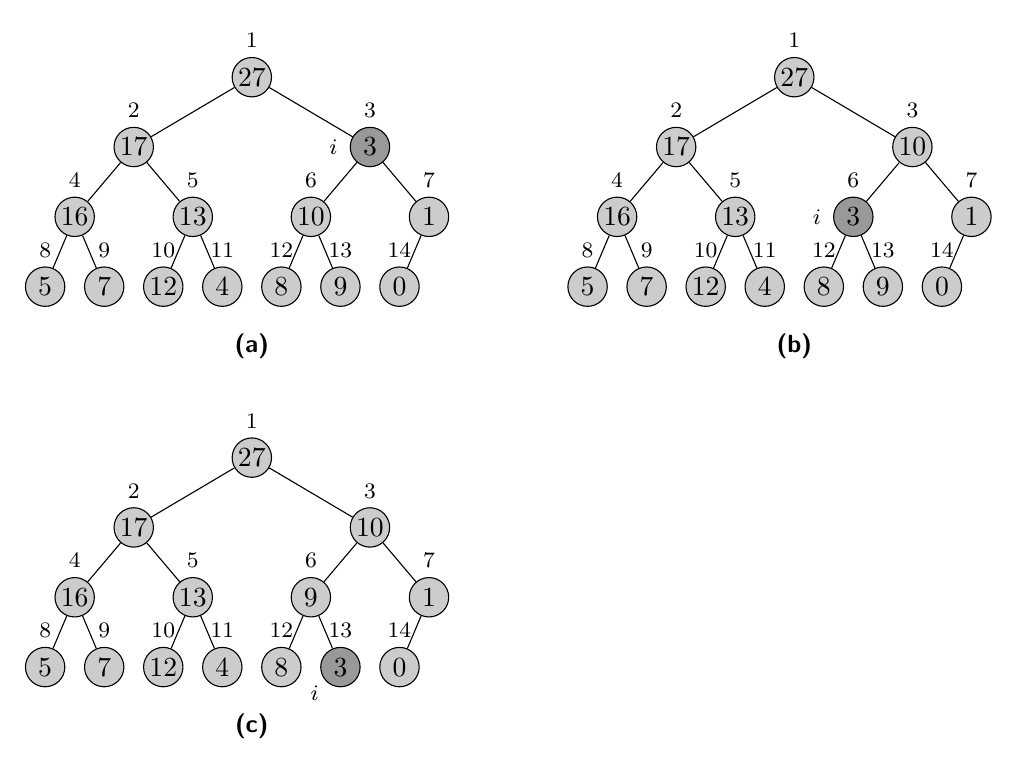
\begin{tikzpicture}[
	pic matrix/.style = {matrix of nodes, column sep=15mm, row sep=5mm, draw=none, fill=none, rectangle},
	level/.style = {level distance=10mm, sibling distance=60mm/2^#1},
	every node/.style = {align=center, inner sep=-1pt, minimum size=5mm, circle, draw, fill=black!20},
	every label/.style = {font=\footnotesize, minimum size=4mm, draw=none, fill=none},
	marked node/.style = {fill=black!40},
	picture label/.style = {font=\small\bfseries\sffamily, draw=none, fill=none}
]

\matrix[pic matrix] (pic) {
	\node[label=1] {27}
		child {node[label=2] {17}
			child {node[label=4] {16}
				child {node[label=8] {5}}
				child {node[label=9] {7}}
			}
			child {node[label=5] {13}
				child {node[label=10] {12}}
				child {node[label=11] (x) {4}}
			}
		}
		child {node[marked node, label=3, label=left:$i$] {3}
			child {node[label=6] {10}
				child {node[label=12] (y) {8}}
				child {node[label=13] {9}}
			}
			child {node[label=7] {1}
				child {node[label=14] {0}}
				child[missing]
			}
		};
	\node[picture label, below=5mm] at ($ (x)!0.5!(y) $) {(a)};
	&
	\node[label=1] {27}
		child {node[label=2] {17}
			child {node[label=4] {16}
				child {node[label=8] {5}}
				child {node[label=9] {7}}
			}
			child {node[label=5] {13}
				child {node[label=10] {12}}
				child {node[label=11] (x) {4}}
			}
		}
		child {node[label=3] {10}
			child {node[marked node, label=6, label=left:$i$] {3}
				child {node[label=12] (y) {8}}
				child {node[label=13] {9}}
			}
			child {node[label=7] {1}
				child {node[label=14] {0}}
				child[missing]
			}
		};
	\node[picture label, below=5mm] at ($ (x)!0.5!(y) $) {(b)};
	\\
	\node[label=1] {27}
		child {node[label=2] {17}
			child {node[label=4] {16}
				child {node[label=8] {5}}
				child {node[label=9] {7}}
			}
			child {node[label=5] {13}
				child {node[label=10] {12}}
				child {node[label=11] (x) {4}}
			}
		}
		child {node[label=3] {10}
			child {node[label=6] {9}
				child {node[label=12] (y) {8}}
				child {node[marked node, label=13, label=below left:{$i$}] {3}}
			}
			child {node[label=7] {1}
				child {node[label=14] {0}}
				child[missing]
			}
		};
	\node[picture label, below=5mm] at ($ (x)!0.5!(y) $) {(c)};
	& \\
};

\end{tikzpicture}

	\caption{Działanie procedury $\proc{Max-Heapify}(A,3)$ dla tablicy $A=\langle$27,\! 17,\! 3,\! 16,\! 13,\! 10,\! 1,\! 5,\! 7,\! 12,\! 4,\! 8,\! 9,\! 0$\rangle$.
{\sffamily\bfseries\doubledash{(a)}{(b)}} Drzewo binarne reprezentujące $A$, w~którym przywracana jest własność kopca typu max, odpowiednio, w~węzłach $i=3$ oraz $i=6$.
{\sffamily\bfseries(c)} Wynikowy kopiec z~przywróconą własnością kopca.} \label{fig:6.2-1}
\end{figure}

\exercise %6.2-2
Poniższy pseudokod prezentuje procedurę przywracania własności kopca typu min.
Ponieważ jedyną modyfikacją w~porównaniu z~procedurą \proc{Max-Heapify} jest zmiana znaków nierówności na przeciwne w~warunkach w~wierszach \ref{li:min-heapify-check1} i~\ref{li:min-heapify-check2}, to czas działania tej procedury jest identyczny z~czasem działania \proc{Max-Heapify}, czyli $\Theta(\lg n)$.
\begin{codebox}
\Procname{$\proc{Min-Heapify}(A,i)$}
\li	$l\gets\proc{Left}(i)$
\li	$r\gets\proc{Right}(i)$
\li	\If $l\le\attrib{A}{heap-size}$ i~$A[l]<A[i]$ \label{li:min-heapify-check1}
\li		\Then $\id{smallest}\gets l$
\li		\Else $\id{smallest}\gets i$
		\End
\li	\If $r\le\attrib{A}{heap-size}$ i~$A[r]<A[\id{smallest}]$ \label{li:min-heapify-check2}
\li		\Then $\id{smallest}\gets r$
		\End
\li	\If $\id{smallest}\ne i$
\li		\Then
			zamień $A[i]\leftrightarrow A[\id{smallest}]$
\li			$\proc{Min-Heapify}(A,\id{smallest})$
		\End
\end{codebox}

\exercise %6.2-3
Jeśli element $A[i]$ jest większy niż jego synowie, to \id{largest} jest ustawiane na $i$ i~warunek z~wiersza 8 nie jest spełniony.
Procedura zakończy więc działanie, nie dokonując żadnej zamiany elementów.

\exercise %6.2-4
Z~\refExercise{6.1-7} mamy, że element o~indeksie $i>\attrib{A}{heap-size}/2$ jest liściem kopca, czyli nie istnieją jego synowie.
W~dwóch pierwszych wierszach procedury \proc{Max-Heapify} obliczone zostaną wartości przekraczające \attrib{A}{heap-size}, więc zmienna \id{largest} przyjmie wartość $i$.
Warunek w~wierszu 8 będzie więc fałszywy i~natychmiast po jego sprawdzeniu procedura zakończy działanie.

\exercise %6.2-5
Iteracyjna wersja procedury \proc{Max-Heapify} została przedstawiona poniżej.
\begin{codebox}
\Procname{$\proc{Iterative-Max-Heapify}(A,i)$}
\li	\While \const{true}
\li		\Do
			$l\gets\proc{Left}(i)$ \label{li:iterative-max-heapify-begin}
\li			$r\gets\proc{Right}(i)$
\li			\If $l\le\attrib{A}{heap-size}$ i~$A[l]>A[i]$
\li				\Then $\id{largest}\gets l$
\li				\Else $\id{largest}\gets i$
				\End
\li			\If $r\le\attrib{A}{heap-size}$ i~$A[r]>A[\id{largest}]$
\li				\Then $\id{largest}\gets r$
				\End \label{li:iterative-max-heapify-end}
\li			\If $\id{largest}=i$ \label{li:iterative-max-heapify-cond}
\li				\Then \Return
				\End
\li			zamień $A[i]\leftrightarrow A[\id{largest}]$
\li			$i\gets\id{largest}$
		\End
\end{codebox}
Działania wykonywane w~wierszach \doubledash{\ref{li:iterative-max-heapify-begin}}{\ref{li:iterative-max-heapify-end}} są identyczne jak w~oryginalnej implementacji procedury.
W~zależności od wyniku testu z~wiersza \ref{li:iterative-max-heapify-cond} procedura kończy działanie albo zamienia elementy $A[i]$ i~$A[\id{largest}]$, po czym symuluje wywołanie rekurencyjne, aktualizując wartość zmiennej $i$ i~wykonując kolejną iterację pętli \kw{while}.

\exercise %6.2-6
Najgorszy przypadek dla procedury \proc{Max-Heapify} zachodzi wówczas, gdy zostanie ona wywołana dla korzenia kopca i~schodzi rekurencyjnie aż do jego ostatniego poziomu.
Najdłuższa ścieżka od korzenia do liścia składa się z~$h=\lfloor\lg n\rfloor$ krawędzi (z~\refExercise{6.1-2}) i~tyle będzie wywołań rekurencyjnych procedury w~najgorszym przypadku.
Koszt pracy wykonanej na każdym poziomie rekursji jest stały, a~więc procedura \proc{Max-Heapify} działa wtedy w~czasie $\Omega(\lg n)$.
Przykładowym drzewem, dla którego procedura wykona opisane operacje, jest takie, w~którym korzeń ma wartość 0, a~każdy inny węzeł ma wartość 1.

\subchapter{Budowanie kopca}

\exercise %6.3-1
Ilustracja działania procedury \proc{Build-Max-Heap} dla tablicy $A$ znajduje się na rys.\ \ref{fig:6.3-1}.
\begin{figure}[ht!]
	\centering \begin{tikzpicture}[
	marked node/.style = {tree node, fill=black!40},
	every label/.style = {index node, draw=none, fill=none},
	outer/.append style = {node distance=9mm and 15mm},
	inner/.style = {draw=none, fill=none, node distance=3mm},
]

\node[outer] (pic a) {
\begin{tikzpicture}
	\node[inner] (pic a1) {
	\begin{tikzpicture}[
		row 1/.style = {nodes={fill=black!20}}
	]
		\matrix[array] (arr) {5 & 3 & 17 & 10 & 84 & 19 & 6 & 22 & 9 \\};
		\node[left=of arr-1-1.west] {$A$};
	\end{tikzpicture}
	};
	\node[inner, below=of pic a1] {
	\begin{tikzpicture}[
		every node/.style = {tree node},
		anchor = center
	]
		\node[label=1] {5}
			child {node[label=2] {3}
				child {node[marked node, label=4, label=left:{$i$}] {10}
					child {node[label=8] {22}}
					child {node[label=9] {9}}
				}
				child {node[label=5] {84}}
			}
			child {node[label=3] {17}
				child {node[label=6] {19}}
				child {node[label=7] {6}
					child[missing]
					child {node[draw=none, fill=none] {} edge from parent[draw=none]}
				}
			};
	\end{tikzpicture}
	};
\end{tikzpicture}
};

\node[outer, right=of pic a.south east, anchor=south west] (pic b) {
\begin{tikzpicture}[
	every node/.style = {tree node},
	anchor = center
]
	\node[label=1] {5}
		child {node[label=2] {3}
			child {node[label=4] {22}
				child {node[label=8] {10}}
				child {node[label=9] {9}}
			}
			child {node[label=5] {84}}
		}
		child {node[marked node, label=3, label=left:{$i$}] {17}
			child {node[label=6] {19}}
			child {node[label=7] {6}
				child[missing]
				child {node[draw=none, fill=none] {} edge from parent[draw=none]}
			}
		};
\end{tikzpicture}
};

\node[outer, below=of pic a] (pic c) {
\begin{tikzpicture}[
	every node/.style = {tree node},
	anchor = center
]
	\node[label=1] {5}
		child {node[marked node, label=2, label=left:{$i$}] {3}
			child {node[label=4] {22}
				child {node[label=8] {10}}
				child {node[label=9] {9}}
			}
			child {node[label=5] {84}}
		}
		child {node[label=3] {19}
			child {node[label=6] {17}}
			child {node[label=7] {6}
				child[missing]
				child {node[draw=none, fill=none] {} edge from parent[draw=none]}
			}
		};
\end{tikzpicture}
};

\node[outer, right=of pic c] (pic d) {
\begin{tikzpicture}[
	every node/.style = {tree node},
	anchor = center
]
	\node[marked node, label=1, label=left:{$i$}] {5}
		child {node[label=2] {84}
			child {node[label=4] {22}
				child {node[label=8] {10}}
				child {node[label=9] {9}}
			}
			child {node[label=5] {3}}
		}
		child {node[label=3] {19}
			child {node[label=6] {17}}
			child {node[label=7] {6}
				child[missing]
				child {node[draw=none, fill=none] {} edge from parent[draw=none]}
			}
		};
\end{tikzpicture}
};

\node[outer, below=of pic c] (pic e) {
\begin{tikzpicture}[
	every node/.style = {tree node},
	anchor = center
]
	\node[label=1] {84}
		child {node[label=2] {22}
			child {node[label=4] {10}
				child {node[label=8] {5}}
				child {node[label=9] {9}}
			}
			child {node[label=5] {3}}
		}
		child {node[label=3] {19}
			child {node[label=6] {17}}
			child {node[label=7] {6}
				child[missing]
				child {node[draw=none, fill=none] {} edge from parent[draw=none]}
			}
		};
\end{tikzpicture}
};

\foreach \x in {a,b,c,d,e} {
	\node[subpicture label, below=-3mm of pic \x] {(\x)};
}

\end{tikzpicture}

	\caption{Działanie procedury \proc{Build-Max-Heap} dla tablicy $A=\langle5,3,17,10,84,19,6,22,9\rangle$.
{\sffamily\bfseries(a)} Tablica $A$ i~reprezentowane przez nią drzewo binarne przed pierwszym wywołaniem \proc{Max-Heapify} z~wiersza 3.
{\sffamily\bfseries\doubledash{(b)}{(d)}} Drzewo przed każdym kolejnym wywołaniem \proc{Max-Heapify}.
{\sffamily\bfseries(e)} Wynikowy kopiec typu max} \label{fig:6.3-1}
\end{figure}

\exercise %6.3-2
Wywołując $\proc{Max-Heapify}(A,i)$, zakładamy, że drzewa o~korzeniach w~$\proc{Left}(i)$ i~$\proc{Right}(i)$ (o~ile istnieją) są kopcami typu max.
Jeżeli podczas budowy kopca procedura \proc{Max-Heapify} byłaby wywoływana dla węzłów o~rosnących indeksach, to nie moglibyśmy zagwarantować, że założenie to jest spełnione, dlatego przetwarzanie odbywa się w~kolejności malejących indeksów.

\exercise %6.3-3
Oznaczmy kopiec przez $T$, a~przez $n_h$ -- ilość węzłów kopca $T$ znajdujących się na wysokości $h$.
Udowodnimy fakt przez indukcję względem $h$.

W~pierwszym kroku indukcji musimy pokazać, że $n_0\le\lceil n/2\rceil$.
W~rzeczywistości udowodnimy, że $n_0=\lceil n/2\rceil$.
Korzystając z~\refExercise{6.1-7}, mamy, że węzły znajdujące się w~$T$ na wysokości 0, czyli jego liście, zajmują pozycje $\lfloor n/2\rfloor+1\twodots n$.
Jest ich zatem
\[
    n_0 = n-(\lfloor n/2\rfloor+1)+1 = n-\lfloor n/2\rfloor = \lceil n/2\rceil.
\]
A~więc przypadek bazowy indukcji jest spełniony.

Załóżmy teraz, że $h>0$ i~że twierdzenie jest spełnione dla węzłów na wysokości $h-1$.
Ponadto niech $T'$ będzie kopcem powstałym z~$T$ po usunięciu z~niego wszystkich jego liści.
Nowy kopiec ma zatem $n'=n-n_0$ węzłów.
Ponieważ w~kroku bazowym pokazaliśmy, że $n_0=\lceil n/2\rceil$, to stąd $n'=n-\lceil n/2\rceil=\lfloor n/2\rfloor$.
Węzły, które w~kopcu $T$ znajdują się na wysokości $h$, w~$T'$ zajmują wysokość $h-1$, więc jeśli oznaczymy przez $n_{h-1}'$ liczbę węzłów na wysokości $h-1$ w~kopcu $T'$, to wówczas będzie $n_h=n_{h-1}'$.
Wykorzystując założenie indukcyjne, dostajemy
\[
    n_h = n_{h-1}' \le \lceil n'\!/2^h\rceil = \lceil\lfloor n/2\rfloor/2^h\rceil \le \lceil(n/2)/2^h\rceil = \lceil n/2^{h+1}\rceil,
\]
co kończy dowód.

\input{sc6.4}
\subchapter{Kolejki priorytetowe}

\exercise %6.5-1
Na rys.\ \ref{fig:6.5-1} został przedstawiony kopiec wejściowy $A$ i~wynikowy kopiec otrzymany w~wyniku działania procedury \proc{Heap-Extract-Max}.
W~wierszu 3 zmiennej \id{max} przypisywana jest maksymalna wartość kopca, czyli 15.
Następnie korzeń otrzymuje wartość 1 i~rozmiar kopca jest pomniejszany o~1.
Po przywróceniu własności kopca w~linii 6 procedura zwraca wartość \id{max}.
\begin{figure}[ht]
	\centering
	\begin{tikzpicture}[
	outer/.append style = {node distance=15mm}
]

\node[outer] (pic a) {
\begin{tikzpicture}[
	every node/.style = {tree node},
	anchor = center
]
	\node {15}
		child {node {13}
			child {node {5}
				child {node {4}}
				child {node {0}}
			}
			child {node {12}
				child {node {6}}
				child {node {2}}
			}
		}
		child {node {9}
			child {node {8}
				child {node {1}}
				child[missing]
			}
			child {node {7}
				child[missing]
				child {node[draw=none, fill=none] {} edge from parent[draw=none]}
			}
		};
\end{tikzpicture}
};

\node[outer, right=of pic a] (pic b) {
\begin{tikzpicture}[
	every node/.style = {tree node},
	anchor = center
]
	\node {13}
		child {node {12}
			child {node {5}
				child {node {4}}
				child {node {0}}
			}
			child {node {6}
				child {node {1}}
				child {node {2}}
			}
		}
		child {node {9}
			child {node {8}}
			child {node {7}
				child[missing]
				child {node[draw=none, fill=none] {} edge from parent[draw=none]}
			}
		};
\end{tikzpicture}
};

\node[subpicture label, below=2mm of pic a] {(a)};
\node[subpicture label, below=2mm of pic b] {(b)};

\end{tikzpicture}

	\caption{Działanie procedury \proc{Heap-Extract-Max} dla kopca $A=\langle15,13,9,5,12,8,7,4,0,6,2,1\rangle$.
{\sffamily\bfseries(a)} Kopiec wejściowy $A$.
{\sffamily\bfseries(b)} Kopiec $A$ po usunięciu maksymalnej wartości i~przywróceniu własności kopca naruszonej przez korzeń, któremu wcześniej przypisano wartość 1.} \label{fig:6.5-1}
\end{figure}

\exercise %6.5-2
Procedura \proc{Max-Heap-Insert} rozpoczyna działanie od dodania do kopca nowego elementu o~wartości $-\infty$.
Wartość ta jest następnie odpowiednio modyfikowana i~element jest umieszczany w~odpowiednim miejscu w~kopcu dzięki wywołaniu \proc{Heap-Increase-Key}.
Działanie procedury $\proc{Max-Heap-Insert}(A,10)$ zostało przedstawione na rys.\ \ref{fig:6.5-2}.
\begin{figure}[ht]
	\begin{center}
		\includegraphics{fig_6.5-2}
	\end{center}
	\caption{Działanie procedury $\proc{Max-Heap-Insert}(A,10)$ dla kopca $A=\langle$15,\! 13,\! 9,\! 5,\! 12,\! 8,\! 7,\! 4,\! 0,\! 6,\! 2,\! 1$\rangle$.
{\sffamily\bfseries(a)} Kopiec po dodaniu nowego elementu o~wartości początkowej $-\infty$.
{\sffamily\bfseries(b)} Działa teraz procedura \proc{Heap-Increase-Key}.
Na rysunku pokazano wartość zmiennej $i$ w~tej procedurze.
Wartość nowego elementu została zwiększona i~wynosi teraz 10.
{\sffamily\bfseries(c)} Po wykonaniu pierwszej iteracji pętli \kw{while} procedury \proc{Heap-Increase-Key} nowy element został zamieniony ze swoim ojcem.
{\sffamily\bfseries(d)} Po drugiej iteracji pętli nastąpiła jeszcze jedna zamiana nowego elementu i~jego aktualnego ojca, dzięki czemu $A$ spełnia już własność kopca i~procedura kończy działanie.} \label{fig:6.5-2}
\end{figure}

\exercise %6.5-3
Zakładamy, że tablica $A$ stanowi kopiec typu min.
Poniższe procedury stanowią implementację kolejki priorytetowej typu min i~działają analogicznie do odpowiadających im procedur dla kolejki priorytetowej typu max.
\begin{codebox}
\Procname{$\proc{Heap-Minimum}(A)$}
\li	\Return $A[1]$
\end{codebox}
\begin{codebox}
\Procname{$\proc{Heap-Extract-Min}(A)$}
\li	\If $\attrib{A}{heap-size}<1$
\li		\Then \Error ,,kopiec pusty''
		\End
\li	$\id{min}\gets A[1]$
\li	$A[1]\gets A[\attrib{A}{heap-size}]$
\li	$\attrib{A}{heap-size}\gets\attrib{A}{heap-size}-1$
\li	$\proc{Min-Heapify}(A,1)$
\li	\Return \id{min}
\end{codebox}
\begin{codebox}
\Procname{$\proc{Heap-Decrease-Key}(A,i,\id{key})$}
\li	\If $\id{key}>A[i]$
\li		\Then \Error ,,nowy klucz jest większy niż klucz aktualny''
		\End
\li	$A[i]\gets\id{key}$
\li	\While $i>1$ i~$A[\proc{Parent}(i)]>A[i]$
\li		\Do
			zamień $A[i]\leftrightarrow A[\proc{Parent}(i)]$
\li			$i\gets\proc{Parent}(i)$
		\End
\end{codebox}
\begin{codebox}
\Procname{$\proc{Min-Heap-Insert}(A,\id{key})$}
\li	$\attrib{A}{heap-size}\gets\attrib{A}{heap-size}+1$
\li	$A[\attrib{A}{heap-size}]\gets\infty$
\li	$\proc{Heap-Decrease-Key}(A,\attrib{A}{heap-size},\id{key})$
\end{codebox}

\exercise %6.5-4
Po wykonaniu wiersza 1 procedury \proc{Max-Heap-Insert} wartość $A[\attrib{A}{heap-size}]$ pozostaje niezdefiniowana i~może zawierać liczbę większą niż \id{key}.
Wówczas jednak wywołanie \proc{Heap-Increase-Key} zakończy się z~błędem.
Radzimy sobie z~tym problemem poprzez nadanie elementowi wartości $-\infty$.

\exercise %6.5-5
\begin{description}
	\item[Inicjowanie:] Przed wykonaniem wiersza3 tablica $A[1\twodots\attrib{A}{heap-size}]$ jest kopcem typu max.
Zwiększenie wartości $A[i]$ może naruszyć własność kopca tylko dla elementów $A[i]$ oraz $A[\proc{Parent}(i)]$.
	\item[Utrzymanie:] Dokonując zamiany elementów w~wiers 5 w~bieżącej iteracji pętli, przywracamy własność kopca dla elementów $A[i]$ oraz $A[\proc{Parent}(i)]$.
Jednak operacja ta może wygenerować nową parę elementów niespełniających własności kopca: $A[\proc{Parent}(i)]$ oraz $A[\proc{Parent}(\proc{Parent}(i))]$.
Aktualizacja wartości $i$ powoduje zachowanie niezmiennika, albowiem nowa para elementów jest jedyną, która może naruszać własność kopca.
	\item[Zakończenie:] Pętla kończy działanie, gdy $i\le1$ lub $A[\proc{Parent}(i)]\ge A[i]$.
W~pierwszym przypadku $\proc{Parent}(i)\le0$, co jest niepoprawną wartością dla indeksów tablicy $A$.
W~drugim natomiast jedyna para, która mogłaby naruszać własność kopca, w~rzeczywistości ją spełnia.
A~zatem po zakończeniu wykonywania pętli tablica $A[1\twodots\attrib{A}{heap-size}]$ stanowi kopiec typu max.
\end{description}
Z~prawdziwości niezmiennika pętli wynika, że procedura \proc{Heap-Increase-Key} poprawnie zwiększa wartość węzła $i$, pozostawiając kopiec typu max.

\exercise %6.5-6
Kolejkę FIFO implementujemy, wykorzystując do tego celu kolejkę priorytetową typu min.
Przy inicjalizacji kolejki będziemy ustawiać wartość dodatkowej zmiennej \id{rank} na 1.
Przed dodaniem nowego elementu do kolejki FIFO nadamy mu rangę, czyli powiążemy go z~aktualną wartością zmiennej \id{rank}, po czym wstawimy element wraz z~jego rangą do kolejki priorytetowej procedurą \proc{Min-Heap-Insert}.
Warunek kolejki priorytetowej spełniany będzie tylko na podstawie wartości rang elementów.
Po umieszczeniu obiektu w~kolejce wartość zmiennej \id{rank} zostanie zwiększona o~1.
Z~kolei usuwanie elementów będzie odbywać się poprzez zwykłe wywołanie procedury \proc{Heap-Extract-Min}.
Taka implementacja operacji na kolejce FIFO zapewnia, że w~danym momencie w~strukturze danych nie będzie dwóch różnych elementów z~tą samą rangą i~elementy pobierane będą w~odpowiedniej kolejności.

Realizacja stosu jest podobna, ale używamy do tego celu kolejki priorytetowej typu max, w~której porównań dokonujemy na rangach związanych z~elementami.
Podczas wstawiania elementów na stos korzystamy z~procedury \proc{Max-Heap-Insert} i~inkrementujemy zmienną \id{rank} (zainicjalizowaną na 1 w~momencie utworzenia stosu).
Usuwanie polega na odnalezieniu i~pobraniu elementu z~największą rangą, co realizowane jest za pomocą \proc{Heap-Extract-Max}.
W~wyniku tego elementy pobierane są w~kolejności odwrotnej do tej, w~której były wstawiane.

\exercise %6.5-7
\note{Zmienimy nazwę operacji z~sugerowanej w~Podręczniku \proc{Heap-Delete} na \proc{Max-Heap-Delete}, aby odróżnić ją od analogicznej procedury dla kopca typu min.}

\noindent Przedstawiona poniżej procedura \proc{Max-Heap-Delete} zamienia element $A[i]$ w~\singledash{$n$}{elementowym} kopcu $A$ typu max z~jego liściem $A[\attrib{A}{heap-size}]$, po czym dekrementuje \attrib{A}{heap-size}.
Po tym kroku własność kopca może być naruszona przez węzeł $A[i]$ na dwa sposoby.
W~pierwszym przypadku mamy sytuację, w~której $A[i]<A[\proc{Left}(i)]$ lub $A[i]<A[\proc{Right}(i)]$ -- przywracamy więc własność kopca za pomocą wywołania \proc{Max-Heapify}.
W~drugim przypadku $A[i]>A[\proc{Parent}(i)]$, więc w~celu odbudowy struktury kopca wystarczy wykonać podobne operacje, jak w~procedurze \proc{Heap-Increase-Key}.
Ostatni krok procedury to zwrócenie elementu, który początkowo zajmował w~kopcu pozycję $i$.
\begin{codebox}
\Procname{$\proc{Max-Heap-Delete}(A,i)$}
\li	zamień $A[i]\leftrightarrow A[\attrib{A}{heap-size}]$
\li	$\attrib{A}{heap-size}\gets\attrib{A}{heap-size}-1$
\li	$\proc{Max-Heapify}(A,i)$ \label{li:max-heap-delete-heapify}
\li	\While $i>1$ i~$A[\proc{Parent}(i)]<A[i]$ \label{li:max-heap-delete-while-begin}
\li		\Do
			zamień $A[i]\leftrightarrow A[\proc{Parent}(i)]$
\li			$i\gets\proc{Parent}(i)$
		\End \label{li:max-heap-delete-while-end}
\li	\Return $A[\attrib{A}{heap-size}+1]$
\end{codebox}

Zarówno wywołanie z~wiersza \ref{li:max-heap-delete-heapify}, jak i~pętla \kw{while} w~wierszach \doubledash{\ref{li:max-heap-delete-while-begin}}{\ref{li:max-heap-delete-while-end}} zajmuje czas $O(\lg n)$, a~więc czasem działania procedury \proc{Max-Heap-Delete} jest również $O(\lg n)$.

\exercise %6.5-8
W~algorytmie wykorzystamy kolejkę priorytetową typu min jako strukturę pomocniczą.
Na początku do kolejki zostaną przeniesione elementy z~głowy każdej listy.
Jest oczywiste, że wśród tych elementów znajduje się najmniejszy element listy wynikowej.
Aby go uzyskać, wystarczy wywołać na kolejce operację \proc{Extract-Min}.
Kolejnego elementu należy szukać wśród aktualnych węzłów kolejki lub w~głowie listy, do której początkowo należało usunięte przed chwilą minimum.
Głowę tej listy, o~ile istnieje, przenosimy do kolejki.
W~kolejnych iteracjach powtarzamy te operacje -- pobieramy najmniejszy element kolejki i~wstawiamy na listę wynikową, po czym uzupełniamy kolejkę głową listy, do której należał pobrany element, o~ile lista ta nie jest jeszcze pusta.
Proces ten powtarzamy aż do opróżnienia kolejki, co następuje po przetworzeniu zawartości wszystkich list.
Aby zachować kolejność niemalejącą na liście wynikowej, musimy wstawiać elementy na jej koniec, pamiętając wskaźnik do ogona tej listy.

Podczas działania algorytmu wykonamy $n$ razy operację wstawienia węzła do kolejki zawierającej co najwyżej $k$ elementów i~tyleż samo operacji \proc{Extract-Min}.
Otrzymujemy zatem górne oszacowanie $O(n\lg k)$ na czas działania algorytmu, przy założeniu, że kolejka priorytetowa została zaimplementowana w~oparciu o~kopiec typu min.


\problems

\problem{Budowa kopca przez wstawianie} %6-1

\subproblem %6-1(a)
Procedury te nie zawsze generują identyczne kopce dla tej samej tablicy wejściowej.
Jeśli na przykład rozważymy tablicę $A=\langle1,2,3\rangle$, to kopce budowane przez obie procedury różnią się, jak to widać na rys.\ \ref{fig:6-1(a)}.
\begin{figure}[!ht]
	\centering \begin{tikzpicture}

\node[outer] (pic a) {
\begin{tikzpicture}[every node/.style = tree node, anchor=center]
	\node {3}
		child {node {2}}
		child {node {1}};
\end{tikzpicture}
};

\node[outer, right=20mm of pic a] (pic b) {
\begin{tikzpicture}[every node/.style = tree node, anchor=center]
	\node {3}
		child {node {1}}
		child {node {2}};
\end{tikzpicture}
};

\node[subpicture label, below=2mm of pic a] {(a)};
\node[subpicture label, below=2mm of pic b] {(b)};

\end{tikzpicture}

	\caption{Porównanie kopców budowanych przez obie procedury dla tablicy $A=\langle1,2,3\rangle$.
{\sffamily\bfseries(a)} Wynik działania \proc{Build-Max-Heap}.
{\sffamily\bfseries(b)} Wynik działania \proc{Build-Max-Heap}$'$.} \label{fig:6-1(a)}
\end{figure}

\subproblem %6-1(b)
Najgorszym przypadkiem dla procedury \proc{Build-Max-Heap}$'$ jest tablica uporządkowana rosnąco.
W~każdym z~$n-1$ wywołań \proc{Max-Heap-Insert} z~wiersza 3 nowy węzeł transportowany jest wówczas aż do korzenia kopca, co wymaga $\Theta(\lg i)$ operacji przy $i$\nbhyphen elementowym kopcu.
Stąd czas działania \proc{Build-Max-Heap}$'$ w~przypadku pesymistycznym wynosi
\[
	\sum_{i=2}^n\Theta(\lg i) = \Theta(\lg(n!)) = \Theta(n\lg n).
\]

\problem{Analiza kopców rzędu $d$} %6-2

\subproblem %6-2(a)
\singledash{$d$}{kopiec} będziemy reprezentować w~tablicy w~następujący sposób.
Podobnie jak w~reprezentacji tablicowej kopców binarnych tablica $A$ reprezentująca \singledash{$d$}{kopiec} będzie mieć atrybuty \attrib{A}{length} oraz \attrib{A}{heap-size}.
Na pierwszej pozycji tablicy znajdzie się korzeń kopca, a~pozycje $2\twodots d+1$ będą zajmowane przez $d$ synów korzenia.
Synowie pierwszego z~lewej syna korzenia zajmą pozycje $d+2\twodots2d+1$, synowie drugiego od lewej syna korzenia -- pozycje $2d+2\twodots3d+1$ itd.
Ogólnie, mając dany indeks węzła $i$, można wyznaczyć indeks jego ojca, korzystając ze wzoru $\lceil(i-1)/d\rceil$.
Uogólnienie procedury \proc{Parent} dla kopca rzędu $d$ wygląda zatem następująco:
\begin{codebox}
\Procname{$\proc{Multiary-Parent}(d,i)$}
\zi	\Return $\lceil(i-1)/d\rceil$
\end{codebox}

Łatwo pokazać, że indeks \singledash{$k$}{tego} od lewej syna węzła o~indeksie $i$, gdzie $k=1$, 2, \dots, $d$, jest opisany wzorem $d(i-1)+k+1$.
Poniższa procedura stanowi uogólnienie procedur \proc{Left} i~\proc{Right} dla kopca rzędu $d$ -- w~porównaniu do nich przyjmuje dodatkowy parametr $k$ oznaczający numer szukanego syna węzła $i$.
\begin{codebox}
\Procname{$\proc{Multiary-Child}(d,k,i)$}
\zi	\Return $d(i-1)+k+1$
\end{codebox}

Można sprawdzić, że zachodzi $\proc{Multiary-Parent}(d,\proc{Multiary-Child}(d,k,i))=i$ dla każdego $k=1$, 2, \dots, $d$.

\subproblem %6-2(b)
Uogólnimy rozumowanie z~\refExercise{6.1-1} na kopce rzędu $d$.
Potraktujmy taki kopiec jak drzewo \singledash{$d$}{arne} o~wysokości $h$ i~$n$ węzłach.
Na \singledash{$i$}{tym} poziomie tego drzewa, gdzie $i=0$, 1, \dots, $h-1$, znajduje się $d^i$ węzłów.
Najniższy, \singledash{$h$}{ty} poziom, może zawierać od 1 do $d^h$ węzłów.
Mamy zatem
\[
    \sum_{i=0}^{h-1}d^i+1 \le n \le \sum_{i=0}^hd^i.
\]
Na podstawie punktu (c) problemu \refProblem{3-1} sumę po lewej stronie można oszacować przez $\Theta(d^{h-1})$, a~sumę po prawej -- przez $\Theta(d^h)$.
Oba te oszacowania dają w~wyniku $h=\Theta(\log_dn)$.

\subproblem %6-2(c)
Przedstawimy najpierw implementację procedury \proc{Max-Heapify} dla kopców rzędu $d$.
Ogólny zarys jej działania pozostaje niezmieniony w~porównaniu z~oryginalną procedurą \proc{Max-Heapify}.
Na każdym poziomie rekursji musimy wyznaczyć maksimum z~$d+1$ wartości -- bieżącego węzła i~jego $d$ synów.
W~tym celu stosujemy pętlę przeglądającą wszystkich synów bieżącego węzła.
\begin{codebox}
\Procname{$\proc{Multiary-Max-Heapify}(A,d,i)$}
\li	$\id{largest}\gets i$
\li	$k\gets1$
\li	$\id{child}\gets\proc{Multiary-Child}(d,1,i)$
\li	\While $k\le d$ i~$\id{child}\le\attrib{A}{heap-size}$ \label{li:multiary-max-heapify-while-begin}
\li		\Do \If $A[\id{child}]>A[\id{largest}]$
\li				\Then $\id{largest}\gets\id{child}$
				\End
\li			$k\gets k+1$
\li			$\id{child}\gets\proc{Multiary-Child}(d,k,i)$ \label{li:multiary-max-heapify-child}
		\End \label{li:multiary-max-heapify-while-end}
\li	\If $\id{largest}\ne i$
\li		\Then zamień $A[i]\leftrightarrow A[\id{largest}]$
\li			$\proc{Multiary-Max-Heapify}(A,d,\id{largest})$
		\End
\end{codebox}
Zauważmy, że podczas wykonywania pętli \kw{while} w~wierszach \doubledash{\ref{li:multiary-max-heapify-while-begin}}{\ref{li:multiary-max-heapify-while-end}} zmienna $k$ może przyjąć wartość $d+1$ i~wówczas w~wierszu \ref{li:multiary-max-heapify-child} zostaje wyznaczony indeks nieistniejącego, \singledash{$(d+1)$}{szego} syna węzła $i$.
Jednak wartości tej nigdzie później nie wykorzystujemy, ponieważ następną operacją jest przerwanie pętli \kw{while}.

Na każdym poziomie rekursji (z~wyjątkiem być może ostatniego) wykonywanych jest $\Theta(d)$ operacji.
Na mocy poprzedniego punktu mamy $\Theta(\log_dn)$ wywołań rekurencyjnych, a~zatem czasem działania powyższej procedury jest $\Theta(d\log_dn)$.

Procedura \proc{Multiary-Heap-Extract-Max}, która implementuje operację \proc{Extract-Max} dla \singledash{$d$}{kopca}, przyjmuje jako parametry kopiec $A$ oraz jego rząd $d$.
Działa ona identyczne jak operacja \proc{Extract-Max} dla kopca binarnego, jednak w~wierszu 6 zamiast procedury \proc{Max-Heapify} wywołuje procedurę \proc{Multiary-Max-Heapify} przedstawioną powyżej.
Czas działania tej operacji wynosi $\Theta(d\log_dn)$.

\subproblem %6-2(d)
Procedura \proc{Multiary-Max-Heap-Insert} implementująca operację \proc{Insert} dla \singledash{$d$}{kopca} przyjmuje na wejściu kopiec $A$, rząd kopca $d$ oraz wartość \id{key}, która będzie wstawiana do $A$.
Jej działanie jest analogiczne do działania procedury wstawiania węzła do kopca binarnego.
Jedyną różnicą jest wiersz \ref{li:multiary-max-heap-insert-increase-key}, który zamiast \proc{Heap-Increase-Key} zawiera analogiczne wywołanie procedury \proc{Multiary-Heap-Increase-Key} zwiększającej wartość węzła w~kopcu rzędu $d$.
\begin{codebox}
\Procname{$\proc{Multiary-Max-Heap-Insert}(A,d,\id{key})$}
\li	$\attrib{A}{heap-size}\gets\attrib{A}{heap-size}+1$
\li	$A[\attrib{A}{heap-size}]\gets-\infty$
\li	$\proc{Multiary-Heap-Increase-Key}(A,d,\attrib{A}{heap-size},\id{key})$ \label{li:multiary-max-heap-insert-increase-key}
\end{codebox}

Czas działania operacji \proc{Insert} dla \singledash{$d$}{kopca} jest tego samego rzędu co czas działania wywołania z~wiersza 3.
Implementacja wywoływanej procedury \proc{Multiary-Heap-Increase-Key} i~analiza jej czasu działania zostały opisane w~następnym punkcie.

\subproblem %6-2(e)
Implementacja tej operacji dla \singledash{$d$}{kopca} jest analogiczna do jej implementacji dla kopca binarnego.
Jednak zamiast sprawdzania poprawności parametru $k$, do $A[i]$ przypisujemy natychmiast odpowiednią wartość.
\begin{codebox}
\Procname{$\proc{Multiary-Heap-Increase-Key}(A,d,i,k)$}
\li	$A[i]\gets\max(A[i],k)$ \label{li:multiary-heap-increase-key}
\li	\While $i>1$ i~$A[\proc{Multiary-Parent}(d,i)]<A[i]$
\li		\Do zamień $A[i]\leftrightarrow A[\proc{Multiary-Parent}(d,i)]$
\li			$i\gets\proc{Multiary-Parent}(d,i)$
		\End
\end{codebox}

Po wykonaniu wiersza \ref{li:multiary-heap-increase-key} wartość węzła $i$ może być większa niż wartość jego ojca.
W~najgorszym przypadku, jeśli węzeł $i$ jest liściem i~jego nowa wartość jest największą wartością w~kopcu, to zostanie on przetransportowany aż do korzenia, co zajmie czas proporcjonalny do wysokości kopca, czyli, na mocy punktu (b), $\Theta(\log_dn)$.

\problem{Tablice Younga} %6-3

\subproblem %6-3(a)
Jedną z~tablic Younga zawierających podane elementy jest
\[
	\begin{pmatrix}
		2 & 3 & 14 & 16 \\
		4 & 8 & \infty & \infty \\
		5 & 12 & \infty & \infty \\
		9 & \infty & \infty & \infty
	\end{pmatrix}.
\]

\subproblem %6-3(b)
Załóżmy, że $Y[1,1]=\infty$ i~że tablica $Y$ nie jest pusta, tzn.\ $Y[i,j]\ne\infty$ dla pewnych $i$, $j$ takich, że $1\le i\le m$ oraz $1\le j\le n$.
Ale z~własności tablicy Younga otrzymujemy, że $Y[1,1]\le Y[1,j]\le Y[i,j]$, co prowadzi do sprzeczności z~założeniem.
A~więc tablica Younga $Y$, w~której $Y[1,1]=\infty$, jest pusta.

Dowód drugiej własności przebiega analogicznie.
Przypuśćmy, że $Y[m,n]\ne\infty$ i~że tablica $Y$ nie jest pełna, tzn.\ $Y[i,j]=\infty$ dla pewnych $i$, $j$, gdzie $1\le i\le m$ oraz $1\le j\le n$.
Wykorzystując własność tablicy Younga, dostajemy $Y[i,j]\le Y[i,n]\le Y[m,n]$, co jest sprzeczne z~założeniem.
Tablica Younga $Y$, w~której $Y[m,n]\ne\infty$, jest pełna.

\subproblem %6-3(c)
Procedura ekstrakcji najmniejszego elementu tablicy Younga $Y$ o~rozmiarach $m\times n$ będzie opierać się o~pomysł z~\proc{Max-Heapify}.
Najmniejszym elementem tablicy $Y$ jest $\mu=Y[1,1]$.
Przetransportujemy go na ostatnią pozycję ostatniego wiersza tablicy, skąd będzie można bezpiecznie go usunąć przy jednoczesnym zachowaniu własności tablicy Younga.
W~tym celu porównajmy $\mu$ z~elementem znajdującym się bezpośrednio na prawo i~elementem bezpośrednio w~dół od niego (o~ile istnieją).
Mniejszy z~nich zamieniany jest następnie z~$\mu$, po czym procedura wywołuje się rekurencyjnie dla podtablicy Younga o~rozmiarach $(m-1)\times n$ albo $m\times(n-1)$, w~której $\mu$ stanowi pierwszy element pierwszej kolumny.
Otrzymując w~wyniku tego postępowania tablicę o~rozmiarach $1\times1$, można usunąć jej jedyny element będący najmniejszym elementem początkowej tablicy Younga (zastępując go wartością $\infty$) i~zwrócić go jako wynik algorytmu.

Opisany sposób został zaimplementowany w~poniższym pseudokodzie.
Aby pobrać minimum z~tablicy Younga $Y$ o~rozmiarach $m\times n$, należy wywołać $\proc{Young-Extract-Min}(Y,m,n,1,1)$.
\begin{codebox}
\Procname{$\proc{Young-Extract-Min}(Y,m,n,i,j)$}
\li	\If $\langle i,j\rangle=\langle m,n\rangle$
\li		\Then
			$\id{min}\gets Y[i,j]$
\li			$Y[i,j]\gets\infty$
\li			\Return \id{min}
		\End
\li	$\langle i',j'\rangle\gets\langle i,j+1\rangle$
\li	\If $i<m$
\li		\Then
			\If $j=n$ lub $Y[i+1,j]<Y[i,j+1]$
\li				\Then $\langle i',j'\rangle\gets\langle i+1,j\rangle$
				\End
		\End
\li	zamień $Y[i,j]\leftrightarrow Y[i',j']$
\li	\Return $\proc{Young-Extract-Min}(Y,m,n,i',j')$
\end{codebox}

Niech $T(p)$ będzie maksymalnym czasem działania powyższego algorytmu dla tablicy Younga $m\times n$, gdzie $p=m+n$ jest łączną liczbą jej kolumn i~wierszy.
W~każdym wywołaniu rekurencyjnym zmniejszamy $p$ o~1, wykonując przy tym czas stały, skąd dostajemy
\[
	T(p) =
	\begin{cases}
		\Theta(1), & \text{jeśli $p=2$}, \\
		T(p-1)+\Theta(1), & \text{jeśli $p>2$}.
	\end{cases}
\]
Łatwo sprawdzić, że rozwiązaniem tej rekurencji jest $T(p)=O(p)=O(m+n)$.

\subproblem %6-3(d)
Podamy najpierw pomocniczą procedurę \proc{Youngify}, która działa analogicznie do \proc{Max-Heapify} i~ma na celu przywrócenie własności tablicy Younga $Y$ naruszoną przez $Y[i,j]$.
Element ten wystarczy porównać z~jego sąsiadem znajdującym się powyżej lub sąsiadem znajdującym się po lewej stronie w~tablicy (o~ile istnieją).
W~zależności od tego, który z~tych trzech elementów jest największy, dokonywana jest odpowiednia zamiana i~procedura wywoływana jest rekurencyjnie.
\begin{codebox}
\Procname{$\proc{Youngify}(Y,i,j)$}
\li	$\langle i',j'\rangle\gets\langle i,j\rangle$
\li	\If $i>1$ i~$Y[i-1,j]>Y[i',j']$
\li		\Then $\langle i',j'\rangle\gets\langle i-1,j\rangle$
		\End
\li	\If $j>1$ i~$Y[i,j-1]>Y[i',j']$
\li		\Then $\langle i',j'\rangle\gets\langle i,j-1\rangle$
		\End
\li	\If $\langle i',j'\rangle\ne\langle i,j\rangle$
\li		\Then
			zamień $Y[i,j]\leftrightarrow Y[i',j']$
\li			$\proc{Youngify}(Y,i',j')$
		\End
\end{codebox}

Ponieważ zakładamy, że tablica Younga $Y$ nie jest pełna, to na mocy punktu (b) mamy $Y[m,n]=\infty$, czyli pozycja ta jest pusta i~można wstawić na nią nowy element.
Wówczas jednak własność tablicy Younga może być naruszona, dlatego korzystamy z~procedury \proc{Youngify} w~celu przywrócenia tej własności.
\begin{codebox}
\Procname{$\proc{Young-Insert}(Y,m,n,\id{key})$}
\li	$Y[m,n]\gets\id{key}$
\li	$\proc{Youngify}(Y,m,n)$
\end{codebox}

Analiza poprawności i~czasu działania procedury \proc{Youngify} opiera się na analizie procedury \proc{Max-Heapify}.
W~każdym kolejnym wywołaniu rekurencyjnym jedna z~liczb, $i$ lub $j$, jest mniejsza o~1.
Koniec działania następuje w~najgorszym przypadku, gdy $i=j=1$, po wykonaniu $O(m+n)$ operacji.
A~zatem czasem działania operacji \proc{Young-Insert} jest również $O(m+n)$.

\subproblem %6-3(e)
Niech $A$ będzie tablicą $n^2$ liczb, które należy posortować.
Poniższy algorytm buduje tablicę Younga $n\times n$ z~liczb tablicy $A$, wykonując na każdej z~nich operację \proc{Young-Insert}.
Następnie liczby te są pobierane w~kolejności niemalejącej dzięki $n^2$ wywołaniom \proc{Young-Extract-Min}.
\begin{codebox}
\Procname{$\proc{Young-Sort}(A)$}
\li	$n\gets\sqrt{\attrib{A}{length}}$
\li	\For $i\gets1$ \To $n^2$
\li		\Do $\proc{Young-Insert}(Y,n,n,A[i])$
		\End
\li	\For $i\gets1$ \To $n^2$
\li		\Do $A[i]\gets\proc{Young-Extract-Min}(Y,n,n,1,1)$
		\End
\end{codebox}

Czas działania obu wywoływanych procedur wynosi $O(n)$, zatem powyższy algorytm działa w~czasie $O(n^3)$.
Jeśli mamy danych $m=n^2$ liczb, to jesteśmy w~stanie posortować je przy użyciu tego algorytmu w~czasie $O(m^{3/2})$.
Jest to lepsza złożoność niż kwadratowa, ale gorsza od złożoności liniowo-logarytmicznej.

\subproblem %6-3(f)
Zbadajmy, jak szukana liczba $v$ ma się do ostatniego elementu pierwszego wiersza tablicy Younga $m\times n$.
Jeśli wartości te są równe, to oczywiście można zakończyć poszukiwania z~rezultatem pozytywnym.
W~przeciwnym przypadku, w~zależności od tego, która z~liczb jest większa, odrzucamy z~dalszych poszukiwań cały pierwszy wiersz lub całą ostatnią kolumnę i~kontynuujemy szukanie $v$ w~otrzymanej podtablicy, która stanowi tablicę Younga $(m-1)\times n$ albo $m\times(n-1)$.
W~momencie uzyskania tablicy pustej wiadomo, że szukanej liczby nie ma w~początkowej tablicy.
\begin{codebox}
\Procname{$\proc{Young-Search}(Y,m,n,v)$}
\li	$i\gets1$
\li	$j\gets n$
\li	\While $i\le m$ i~$j\ge1$
\li		\Do
			\If $v=Y[i,j]$
\li				\Then \Return \const{true}
				\End
\li			\If $v>Y[i,j]$
\li				\Then $i\gets i+1$
\li				\Else $j\gets j-1$
				\End
		\End
\li	\Return \const{false}
\end{codebox}

W~każdym kroku pętli \kw{while} zmniejszamy o~1 liczbę kolumn lub liczbę wierszy rozważanej tablicy, wykonując przy tym stałą liczbę operacji -- jasne jest zatem, że czas działania algorytmu wynosi $O(m+n)$.


\chapter{Quicksort -- sortowanie szybkie}

\makeatletter
\def\input@path{{chapter07/}}
\makeatother

\subchapter{Opis algorytmu}

\exercise %7.1-1
\note{Rozwiązanie dotyczy przykładu z~tekstu oryginalnego.}

\noindent Rys.\ \ref{fig:7.1-1} przedstawia działanie procedury \proc{Partition} dla tablicy $A$.
\begin{figure}[ht]
	\centering \begin{tikzpicture}[
	light cell/.style = {row 1 column #1/.style={nodes={fill=black!20}}},
	med cell/.style = {row 1 column #1/.style={nodes={fill=black!40}}},
	index node/.append style = {node distance=1mm and 1mm},
	partition line/.style = {line width=2pt, line cap=rect},
	outer/.append style = {node distance=4mm and 14mm}
]

\node[outer] (pic a) {
\begin{tikzpicture}
	\matrix[array] (arr) {13 & 19 & 9 & 5 & 12 & 8 & 7 & 4 & 21 & 2 & 6 & 11 \\};
	\draw[partition line] (arr-1-1.north west) -- (arr-1-1.south west);
	\draw[partition line] (arr-1-11.north east) -- (arr-1-11.south east);
	\node[index node, above left=of arr-1-1] {$i$};
	\node[index node, above=of arr-1-1] {$p,j$};
	\node[index node, above=of arr-1-12] {$r$};
\end{tikzpicture}
};

\node[outer, below=of pic a] (pic b) {
\begin{tikzpicture}
	\matrix[
		array,
		med cell/.list = {1}
	] (arr) {13 & 19 & 9 & 5 & 12 & 8 & 7 & 4 & 21 & 2 & 6 & 11 \\};
	\draw[partition line] (arr-1-1.north west) -- (arr-1-1.south west);
	\draw[partition line] (arr-1-2.north west) -- (arr-1-2.south west);
	\draw[partition line] (arr-1-12.north west) -- (arr-1-12.south west);
	\node[index node, above left=of arr-1-1] {$i$};
	\node[index node, above=of arr-1-1] {$p$};
	\node[index node, above=of arr-1-2] {$j$};
	\node[index node, above=of arr-1-12] {$r$};
\end{tikzpicture}
};

\node[outer, below=of pic b] (pic c) {
\begin{tikzpicture}
	\matrix[
		array,
		med cell/.list = {1,2}
	] (arr) {13 & 19 & 9 & 5 & 12 & 8 & 7 & 4 & 21 & 2 & 6 & 11 \\};
	\draw[partition line] (arr-1-1.north west) -- (arr-1-1.south west);
	\draw[partition line] (arr-1-3.north west) -- (arr-1-3.south west);
	\draw[partition line] (arr-1-12.north west) -- (arr-1-12.south west);
	\node[index node, above left=of arr-1-1] {$i$};
	\node[index node, above=of arr-1-1] {$p$};
	\node[index node, above=of arr-1-3] {$j$};
	\node[index node, above=of arr-1-12] {$r$};
\end{tikzpicture}
};

\node[outer, below=of pic c.south east, anchor=north east] (pic d) {
\begin{tikzpicture}
	\matrix[
		array,
		light cell/.list = {1},
		med cell/.list = {2,3}
	] (arr) {9 & 19 & 13 & 5 & 12 & 8 & 7 & 4 & 21 & 2 & 6 & 11 \\};
	\draw[partition line] (arr-1-2.north west) -- (arr-1-2.south west);
	\draw[partition line] (arr-1-4.north west) -- (arr-1-4.south west);
	\draw[partition line] (arr-1-12.north west) -- (arr-1-12.south west);
	\node[index node, above=of arr-1-1] {$p,i$};
	\node[index node, above=of arr-1-4] {$j$};
	\node[index node, above=of arr-1-12] {$r$};
\end{tikzpicture}
};

\node[outer, below=of pic d] (pic e) {
\begin{tikzpicture}
	\matrix[
		array,
		light cell/.list = {1,2},
		med cell/.list = {3,4}
	] (arr) {9 & 5 & 13 & 19 & 12 & 8 & 7 & 4 & 21 & 2 & 6 & 11 \\};
	\draw[partition line] (arr-1-3.north west) -- (arr-1-3.south west);
	\draw[partition line] (arr-1-5.north west) -- (arr-1-5.south west);
	\draw[partition line] (arr-1-12.north west) -- (arr-1-12.south west);
	\node[index node, above=of arr-1-1] {$p$};
	\node[index node, above=of arr-1-2] {$i$};
	\node[index node, above=of arr-1-5] {$j$};
	\node[index node, above=of arr-1-12] {$r$};
\end{tikzpicture}
};

\node[outer, below=of pic e] (pic f) {
\begin{tikzpicture}
	\matrix[
		array,
		light cell/.list = {1,2},
		med cell/.list = {3,4,5}
	] (arr) {9 & 5 & 13 & 19 & 12 & 8 & 7 & 4 & 21 & 2 & 6 & 11 \\};
	\draw[partition line] (arr-1-3.north west) -- (arr-1-3.south west);
	\draw[partition line] (arr-1-6.north west) -- (arr-1-6.south west);
	\draw[partition line] (arr-1-12.north west) -- (arr-1-12.south west);
	\node[index node, above=of arr-1-1] {$p$};
	\node[index node, above=of arr-1-2] {$i$};
	\node[index node, above=of arr-1-6] {$j$};
	\node[index node, above=of arr-1-12] {$r$};
\end{tikzpicture}
};

\node[outer, below=of pic f] (pic g) {
\begin{tikzpicture}
	\matrix[
		array,
		light cell/.list = {1,2,3},
		med cell/.list = {4,5,6}
	] (arr) {9 & 5 & 8 & 19 & 12 & 13 & 7 & 4 & 21 & 2 & 6 & 11 \\};
	\draw[partition line] (arr-1-4.north west) -- (arr-1-4.south west);
	\draw[partition line] (arr-1-7.north west) -- (arr-1-7.south west);
	\draw[partition line] (arr-1-12.north west) -- (arr-1-12.south west);
	\node[index node, above=of arr-1-1] {$p$};
	\node[index node, above=of arr-1-3] {$i$};
	\node[index node, above=of arr-1-7] {$j$};
	\node[index node, above=of arr-1-12] {$r$};
\end{tikzpicture}
};

\node[outer, right=of pic a.east] (pic h) {
\begin{tikzpicture}
	\matrix[
		array,
		light cell/.list = {1,2,3,4},
		med cell/.list = {5,6,7}
	] (arr) {9 & 5 & 8 & 7 & 12 & 13 & 19 & 4 & 21 & 2 & 6 & 11 \\};
	\draw[partition line] (arr-1-5.north west) -- (arr-1-5.south west);
	\draw[partition line] (arr-1-8.north west) -- (arr-1-8.south west);
	\draw[partition line] (arr-1-12.north west) -- (arr-1-12.south west);
	\node[index node, above left=of arr-1-1] {};
	\node[index node, above=of arr-1-1] {$p$};
	\node[index node, above=of arr-1-4] {$i$};
	\node[index node, above=of arr-1-8] {$j$};
	\node[index node, above=of arr-1-12] {$r$};
\end{tikzpicture}
};

\node[outer, below=of pic h.south east, anchor=north east] (pic i) {
\begin{tikzpicture}
	\matrix[
		array,
		light cell/.list = {1,2,3,4,5},
		med cell/.list = {6,7,8}
	] (arr) {9 & 5 & 8 & 7 & 4 & 13 & 19 & 12 & 21 & 2 & 6 & 11 \\};
	\draw[partition line] (arr-1-6.north west) -- (arr-1-6.south west);
	\draw[partition line] (arr-1-9.north west) -- (arr-1-9.south west);
	\draw[partition line] (arr-1-12.north west) -- (arr-1-12.south west);
	\node[index node, above=of arr-1-1] {$p$};
	\node[index node, above=of arr-1-5] {$i$};
	\node[index node, above=of arr-1-9] {$j$};
	\node[index node, above=of arr-1-12] {$r$};
\end{tikzpicture}
};

\node[outer, below=of pic i] (pic j) {
\begin{tikzpicture}
	\matrix[
		array,
		light cell/.list = {1,2,3,4,5},
		med cell/.list = {6,7,8,9}
	] (arr) {9 & 5 & 8 & 7 & 4 & 13 & 19 & 12 & 21 & 2 & 6 & 11 \\};
	\draw[partition line] (arr-1-6.north west) -- (arr-1-6.south west);
	\draw[partition line] (arr-1-10.north west) -- (arr-1-10.south west);
	\draw[partition line] (arr-1-12.north west) -- (arr-1-12.south west);
	\node[index node, above=of arr-1-1] {$p$};
	\node[index node, above=of arr-1-5] {$i$};
	\node[index node, above=of arr-1-10] {$j$};
	\node[index node, above=of arr-1-12] {$r$};
\end{tikzpicture}
};

\node[outer, below=of pic j] (pic k) {
\begin{tikzpicture}
	\matrix[
		array,
		light cell/.list = {1,2,3,4,5,6},
		med cell/.list = {7,8,9,10}
	] (arr) {9 & 5 & 8 & 7 & 4 & 2 & 19 & 12 & 21 & 13 & 6 & 11 \\};
	\draw[partition line] (arr-1-7.north west) -- (arr-1-7.south west);
	\draw[partition line] (arr-1-11.north west) -- (arr-1-11.south west);
	\draw[partition line] (arr-1-12.north west) -- (arr-1-12.south west);
	\node[index node, above=of arr-1-1] {$p$};
	\node[index node, above=of arr-1-6] {$i$};
	\node[index node, above=of arr-1-11] {$j$};
	\node[index node, above=of arr-1-12] {$r$};
\end{tikzpicture}
};

\node[outer, below=of pic k] (pic l) {
\begin{tikzpicture}
	\matrix[
		array,
		light cell/.list = {1,2,3,4,5,6,7},
		med cell/.list = {8,9,10,11}
	] (arr) {9 & 5 & 8 & 7 & 4 & 2 & 6 & 12 & 21 & 13 & 19 & 11 \\};
	\draw[partition line] (arr-1-8.north west) -- (arr-1-8.south west);
	\draw[partition line] (arr-1-12.north west) -- (arr-1-12.south west);
	\node[index node, above=of arr-1-1] {$p$};
	\node[index node, above=of arr-1-7] {$i$};
	\node[index node, above=of arr-1-12] {$r,j$};
\end{tikzpicture}
};

\node[outer, below=of pic l] (pic m) {
\begin{tikzpicture}
	\matrix[
		array,
		light cell/.list = {1,2,3,4,5,6,7},
		med cell/.list = {9,10,11,12}
	] (arr) {9 & 5 & 8 & 7 & 4 & 2 & 6 & 11 & 21 & 13 & 19 & 12 \\};
	\draw[partition line] (arr-1-8.north west) -- (arr-1-8.south west);
	\draw[partition line] (arr-1-9.north west) -- (arr-1-9.south west);
	\draw[partition line] (arr-1-12.north east) -- (arr-1-12.south east);
	\node[index node, above=of arr-1-1] {$p$};
	\node[index node, above=of arr-1-7] {$i$};
	\node[index node, above=of arr-1-12] {$r$};
\end{tikzpicture}
};

\node[subpicture label, left=1mm of pic a.south west, anchor=south] (label a) {(a)};
\foreach \x in {b,c,d,e,f,g} {
	\node[subpicture label, anchor=south] at (label a |- pic \x.south west) {(\x)};
}

\node[subpicture label, left=1mm of pic h.south west, anchor=south] (label h) {(h)};
\foreach \x in {i,j,k,l,m} {
	\node[subpicture label, anchor=south] at (label h |- pic \x.south west) {(\x)};
}

\end{tikzpicture}

	\caption{Działanie procedury \proc{Partition} dla tablicy $A=\langle13,19,9,5,12,8,7,4,21,2,6,11\rangle$.
{\sffamily\bfseries(a)} Tablica wejściowa z~zaznaczonymi początkowymi wartościami zmiennych.
{\sffamily\bfseries\doubledash{(b)}{(l)}} Kolejne iteracje pętli \kw{for} w~wierszach \doubledash{3}{6}.
{\sffamily\bfseries(m)} Wynikowa tablica $A$ po wykonaniu zamiany z~wiersza 7.} \label{fig:7.1-1}
\end{figure}

\exercise %7.1-2
\note{Poprawną wartością dla\/ $q$ z~treści zadania powinno być\/ $\lfloor(p+r)/2\rfloor$.}

\noindent Zauważmy, że jeśli wszystkie elementy podtablicy $A[p\twodots r]$ mają taką samą wartość, to warunek z~wiersza 4 procedury \proc{Partition} jest spełniony w~każdej iteracji pętli \kw{for}.
Oznacza to, że po wykonaniu tej pętli będzie $i=r-1$ i~procedura zwróci $q=r$.

Odpowiedniej modyfikacji procedury dokonujemy poprzez wprowadzenie licznika elementów równych elementowi rozdzielającemu w~badanej podtablicy.
W~każdej iteracji pętli \kw{for} sprawdzamy dodatkowo, czy $A[j]=x$ i~jeśli tak, to licznik ten inkrementujemy.
Jeśli na końcu procedury jego wartość jest równa $r-p+1$, czyli rozmiarowi podtablicy, to zwracamy $q=\lfloor(p+r)/2\rfloor$.

\exercise %7.1-3
Podczas przetwarzania podtablicy $A[p\twodots r]$ o~rozmiarze $n=r-p+1$ wykonywanych jest $n-1$ iteracji pętli \kw{for}, a~każda z~nich przeprowadza operacje zajmujące czas stały.
Stąd czas działania procedury \proc{Partition} wynosi $\Theta(n)$.

\exercise %7.1-4
W~warunku z~wiersza 4 procedury \proc{Partition} wystarczy zmienić znak nierówności na przeciwny.

\input{sc7.2}
\input{sc7.3}
\input{sc7.4}

\problems

\problem{Poprawność algorytmu podziału Hoare'a} %7-1

\subproblem %7-1(a)
Działanie procedury \proc{Hoare-Partition} dla przykładowej tablicy $A$ zostało przedstawione na rys.\ \ref{fig:7-1a}.
\begin{figure}[!ht]
	\centering \def\scopevdist{-15mm}

\begin{tikzpicture}[
	array/.style = {matrix of nodes, column sep=-\pgflinewidth, nodes={draw, minimum size=5mm, inner sep=0pt, text height=1.5ex}},
	light cell/.style = {row 1 column #1/.style={nodes={fill=black!20}}},
	med cell/.style = {row 1 column #1/.style={nodes={fill=black!40}}},
	index node/.style = {font=\scriptsize, inner sep=0pt, minimum size=5mm, inner sep=0pt, text height=1.5ex},
	partition line/.style = {line width=2pt, line cap=rect},
	picture label/.style = {font=\small\bfseries\sffamily},
	node distance = 5mm and 5mm,
	on grid
]

\begin{scope}
	\matrix[array] (arr) {13 & 19 & 9 & 5 & 12 & 8 & 7 & 4 & 11 & 2 & 6 & 21 \\};
	\draw[partition line] (arr-1-1.north west) -- (arr-1-1.south west);
	\draw[partition line] (arr-1-12.north east) -- (arr-1-12.south east);
	\node[index node, above left=of arr-1-1] {$i$};
	\node[index node, above=of arr-1-1] {$p$};
	\node[index node, above=of arr-1-12] {$r$};
	\node[index node, above right=of arr-1-12] {$j$};
	\node[picture label, left=1 of arr-1-1] {(a)};
\end{scope}

\begin{scope}[yshift=\scopevdist]
	\matrix[
		array,
		light cell/.list = {1},
		med cell/.list = {11,12}
	] (arr) {6 & 19 & 9 & 5 & 12 & 8 & 7 & 4 & 11 & 2 & 13 & 21 \\};
	\draw[partition line] (arr-1-2.north west) -- (arr-1-2.south west);
	\draw[partition line] (arr-1-11.north west) -- (arr-1-11.south west);
	\node[index node, above=of arr-1-1] {$p,i$};
	\node[index node, above=of arr-1-11] {$j$};
	\node[index node, above=of arr-1-12] {$r$};
	\node[picture label, left=1 of arr-1-1] {(b)};
\end{scope}

\begin{scope}[yshift=2*\scopevdist]
	\matrix[
		array,
		light cell/.list = {1,2},
		med cell/.list = {10,11,12}
	] (arr) {6 & 2 & 9 & 5 & 12 & 8 & 7 & 4 & 11 & 19 & 13 & 21 \\};
	\draw[partition line] (arr-1-3.north west) -- (arr-1-3.south west);
	\draw[partition line] (arr-1-10.north west) -- (arr-1-10.south west);
	\node[index node, above=of arr-1-1] {$p$};
	\node[index node, above=of arr-1-2] {$i$};
	\node[index node, above=of arr-1-10] {$j$};
	\node[index node, above=of arr-1-12] {$r$};
	\node[picture label, left=1 of arr-1-1] {(c)};
\end{scope}

\begin{scope}[yshift=3*\scopevdist]
	\matrix[
		array,
		light cell/.list = {1,2,3,4,5,6,7,8,9},
		med cell/.list = {10,11,12}
	] (arr) {6 & 2 & 9 & 5 & 12 & 8 & 7 & 4 & 11 & 19 & 13 & 21 \\};
	\draw[partition line] (arr-1-10.north west) -- (arr-1-10.south west);
	\node[index node, above=of arr-1-1] {$p$};
	\node[index node, above=of arr-1-9] {$j$};
	\node[index node, above=of arr-1-10] {$i$};
	\node[index node, above=of arr-1-12] {$r$};
	\node[picture label, left=1 of arr-1-1] {(d)};
\end{scope}

\end{tikzpicture}

	\caption{Działanie procedury \proc{Hoare-Partition} dla tablicy $A=\langle13,19,9,5,12,8,7,4,11,2,6,21\rangle$.
Wszystkie elementy jasnoszare stanowią obszar złożony z~wartości nie większych niż $x$.
Ciemnoszare elementy tworzą obszar złożony z~wartości nie mniejszych niż $x$.
{\sffamily\bfseries(a)} Wejściowa tablica wraz z~początkowym ustawieniem zmiennych.
{\sffamily\bfseries\doubledash{(b)}{(d)}} Tablica i~bieżące wartości zmiennych po wykonaniu, odpowiednio, jednej, dwóch i~trzech iteracji pętli \kw{while} w~wierszach \doubledash{4}{11}.} \label{fig:7-1a}
\end{figure}

\subproblem %7-1(b)
W~pierwszej iteracji pętli \kw{while} zmienna $j$ zatrzyma się na pewnym indeksie $q\ge p$, a~zmienna $i$ pozostanie na indeksie $p$, pod którym przechowywana jest wartość $x$.
Jeśli $i=j$, to procedura kończy działanie, załóżmy więc, że $i<j$.
Element $A[i]=A[p]=x$ zostanie zamieniony z~$A[q]$.
W~kolejnych iteracjach pętli \kw{while} zmienna $i$ może dotrzeć najdalej na indeks $q$, natomiast $j$ nie będzie nigdy mniejsze niż $p$, bo $A[p]$ zawiera teraz wartość mniejszą bądź równą $x$.
Ponieważ $q>p$, to w~pewnym momencie podczas działania pętli indeksy $i$ i~$j$ miną się, czyli będzie $i\ge j$, co spowoduje przerwanie pętli w~wierszu 11.

\subproblem %7-1(c)
\note{Zakładamy, że podtablica\/ $A[p\twodots r]$ składa się z~co najmniej dwóch elementów.}

\noindent Fakt udowodniony w~punkcie (b) mówi o~tym, że $p\le j\le r$.
Załóżmy, że $A[r]\le x$, bowiem w~przeciwnym przypadku $j<r$ już po pierwszej iteracji pętli \kw{while}.
W~pierwszej iteracji element $A[p]$ jest zamieniany z~$A[r]$, po czym w~kolejnych iteracjach indeks $j$ jest zmniejszany i~również w~tym przypadku mamy $j<r$.

\subproblem %7-1(d)
Wynika to z~warunków stopu obu pętli \kw{repeat} i~testu z~wiersza 9.
Każda para elementów tablicy, która tworzyła inwersję, jest odwracana, dzięki czemu elementy, które naruszały warunek posortowania, po zamianie będą znajdować się w~odpowiednich obszarach tablicy.
Jak tylko indeksy $i$ i~$j$ miną się, każdy element z~podtablicy $A[p\twodots j]$ będzie równy bądź mniejszy od każdego elementu z~$A[j+1\twodots r]$.

\subproblem %7-1(e)
Jedyną różnicą w~porównaniu z~procedurą \proc{Quicksort} jest to, że element rozdzielający nie znajduje się w~$A[q]$ po wykonaniu \proc{Hoare-Partition}, musimy więc sortować rekurencyjnie fragment $A[p\twodots q]$ zamiast $A[p\twodots q-1]$.
Pseudokod procedury został przedstawiony poniżej.
\begin{codebox}
\Procname{$\proc{Hoare-Quicksort}(A,p,r)$}
\li	\If $p<r$
\li		\Then
			$q\gets\proc{Hoare-Partition}(A,p,r)$
\li			$\proc{Hoare-Quicksort}(A,p,q)$
\li			$\proc{Hoare-Quicksort}(A,q+1,r)$
		\End
\end{codebox}

\problem{Alternatywna analiza algorytmu quicksort} %7-2

\subproblem %7-2(a)
W~procedurze \proc{Randomized-Partition} element $A[r]$ jest zamieniany z~elementem wybranym losowo z~podtablicy $A[p\twodots r]$ o~rozmiarze $n=r-p+1$.
Stąd szanse, że dany element tej podtablicy stanie się elementem rozdzielającym, wynoszą $1/n$.
Wobec tego wartość oczekiwana zmiennej $X_i$, gdzie $i=1$, 2, \dots, $n$, wynosi $\E(X_i)=\Pr(X_i=1)=1/n$.

\subproblem %7-2(b)
Wywołanie procedury \proc{Randomized-Quicksort} dla tablicy wejściowej $A$ o~rozmiarze $n$ potrzebuje czasu $\Theta(n)$ na podział tablicy.
Zostaje wyznaczony indeks $q$, gdzie $1\le q\le n$, po czym procedura jest wywoływana rekurencyjnie dla podtablic rozmiarów $q-1$ i~$n-q$.
Zmienna losowa $X_i$ zdefiniowana w~punkcie (a) przyjmuje wartość 1, gdy $i=q$, a~0 w~pozostałych przypadkach.
Stąd czas potrzebny na posortowanie $n$\nbhyphen elementowej tablicy wyraża się wzorem
\[
	T(n) = T(q-1)+T(n-q)+\Theta(n) = \sum_{i=1}^nX_i(T(i-1)+T(n-i)+\Theta(n)).
\]
Biorąc wartości oczekiwane skrajnych wyrażeń, otrzymujemy wzór (7.5) na oczekiwany czas działania algorytmu quicksort.

\subproblem %7-2(c)
\note{W~tekście oryginalnym we wzorze (7.6) sumowanie przebiega od\/ $q=2$.}

\noindent Wykorzystując części (a) i~(b) oraz liniowość wartości oczekiwanej, otrzymujemy:
\begin{align*}
	\E(T(n)) &= \sum_{q=1}^n\E\bigl(X_q(T(q-1)+T(n-q)+\Theta(n))\bigr) \\
	&= \sum_{q=1}^n\E(X_q)\bigl(\E(T(q-1))+\E(T(n-q))+\E(\Theta(n))\bigr) \\
	&= \sum_{q=1}^n\frac{1}{n}\bigl(2\E(T(q-1)))+\Theta(n)\bigr) \\
	&= \frac{2}{n}\sum_{q=2}^{n-1}\E(T(q))+\frac{2}{n}\bigl(\E(T(0))+\E(T(1))\bigr)+\frac{1}{n}\sum_{q=1}^n\Theta(n) \\
	&= \frac{2}{n}\sum_{q=2}^{n-1}\E(T(q))+\Theta(n).
\end{align*}
Skorzystaliśmy z~obserwacji, że składnik $2(\E(T(0))+\E(T(1)))/n$ jest ograniczony przez stałą i~może być wchłonięty przez $\Theta(n)$.

\subproblem %7-2(d)
\note{W~tekście oryginalnym we wzorze (7.7) sumowanie przebiega od\/ $k=2$.}

\noindent Przyjmiemy, że $n>2$ i~rozważymy równoważną sumę od $k=1$, bowiem $1\cdot\lg1=0$.
Rozbijamy ją na dwie części:
\[
	\sum_{k=1}^{n-1}k\lg k = \sum_{k=1}^{\lceil n/2\rceil-1}k\lg k+\sum_{k=\lceil n/2\rceil}^{n-1}k\lg k,
\]
po czym zauważamy, że czynnik $\lg k$ w~pierwszej sumie po prawej stronie znaku równości możemy ograniczyć z~góry przez $\lg(n/2)=\lg n-1$, a~czynnik $\lg k$ w~drugiej sumie -- przez $\lg n$.
Stąd
\begin{align*}
	\sum_{k=1}^{n-1}k\lg k &\le (\lg n-1)\sum_{k=1}^{\lceil n/2\rceil-1}k+\lg n\sum_{k=\lceil n/2\rceil}^{n-1}k \\
	&= \lg n\sum_{k=1}^{n-1}k-\sum_{k=1}^{\lceil n/2\rceil-1}k \\[2mm]
	&\le \frac{n(n-1)\lg n}{2}-\frac{n}{4}\biggl(\frac{n}{2}-1\biggr) \\
	&= \frac{n^2\lg n}{2}-\frac{n\lg n}{2}-\frac{n^2}{8}+\frac{n}{4} \\[1mm]
	&\le \frac{n^2\lg n}{2}-\frac{n^2}{8},
\end{align*}
przy czym ostatnia nierówność zachodzi dla $n\ge\sqrt{2}$.

\subproblem %7-2(e)
Załóżmy, że $n>2$ i~przyjmijmy założenie indukcyjne $\E(T(q))\le aq\lg q$ dla każdego $q=2$, 3, \dots, $n-1$ oraz pewnej stałej $a>0$.
Z~punktu (c) mamy
\[
	\E(T(n)) = \frac{2}{n}\sum_{q=2}^{n-1}\E(T(q))+\Theta(n) \le \frac{2a}{n}\sum_{q=2}^{n-1}q\lg q+\Theta(n).
\]
Wykorzystując teraz nierówność (7.7), dostajemy
\[
	\E(T(n)) \le \frac{2a}{n}\biggl(\frac{n^2\lg n}{2}-\frac{n^2}{8}\biggr)+\Theta(n) = an\lg n-\frac{an}{4}+\Theta(n) \le an\lg n,
\]
gdyż możemy tak zwiększyć $a$, by wyrażenie $an/4$ dominowało nad składnikiem $\Theta(n)$.

Jeśli przyjmiemy, że $\E(T(2))=1$, to wówczas nierówność $\E(T(2))\le a\cdot2\cdot\lg2=2a$ będzie zachodzić, o~ile $a\ge1/2$.
A~zatem można przyjąć $n=2$ na podstawę indukcji i~dowód faktu, że $\E(T(n))=O(n\lg n)$ jest zakończony.
Łącząc ten wynik z~oszacowaniem $\Omega(n\lg n)$ dla przypadku optymistycznego, które zostało wyznaczone w~\refExercise{7.4-2}, dostajemy, że oczekiwanym czasem działania algorytmu quicksort jest $\Theta(n\lg n)$.

\problem{Nieefektywne sortowanie} %7-3

\subproblem %7-3(a)
Udowodnimy poprawność algorytmu przez indukcję względem rozmiaru tablicy $n$.
Łatwo sprawdzić, że algorytm działa poprawnie w~przypadku, gdy $n\le2$.
Załóżmy więc, że $n>2$ i~że poprawnie sortowane są tablice o~rozmiarach mniejszych niż $n$.
W~wyniku wykonania wiersza 6 na pozycjach $\lfloor n/3\rfloor+1\twodots n-\lfloor n/3\rfloor$ znajdują się elementy nie mniejsze od tych z~pozycji $1\twodots\lfloor n/3\rfloor$.
A~zatem, po wykonaniu wiersza 7, $\lfloor n/3\rfloor$ największych elementów tablicy $A$ znajduje się w~obszarze $A[n-\lfloor n/3\rfloor+1\twodots n]$.
Aby zakończyć sortowanie tablicy $A$, wystarczy uporządkować fragment $A[1\twodots n-\lfloor n/3\rfloor]$, co realizuje wiersz 8.

\subproblem %7-3(b)
Procedura jest wywoływana rekurencyjnie 3 razy, zaś każde wywołanie otrzymuje tablicę o~rozmiarze około $2/3$ rozmiaru oryginalnej tablicy.
Ponadto praca poza wywołaniami rekurencyjnymi jest wykonywana w~czasie stałym.
Stąd dostajemy równanie rekurencyjne
\[
	T(n) =
	\begin{cases}
		\Theta(1), & \text{jeśli $n\le2$}, \\
		3T(2n/3)+\Theta(1), & \text{jeśli $n>2$},
	\end{cases}
\]
które rozwiązujemy przy użyciu twierdzenia o~rekurencji uniwersalnej, otrzymując wynik $T(n)=\Theta(n^{\log_{3/2}3})\approx \Theta(n^{2{,}71})$.

\subproblem %7-3(c)
Pesymistyczny czas działania algorytmu \proc{Stooge-Sort} jest wyższego rzędu nie tylko od pesymistycznego czasu działania algorytmów sortowania przez scalanie, kopcowanie czy sortowania szybkiego, ale również od mniej efektywnego sortowania przez wstawianie.
Metoda sortowania profesorów jest więc poprawna, ale bardzo powolna.

\problem{Głębokość stosu w~algorytmie quicksort} %7-4

\subproblem %7-4(a)
\proc{Quicksort}$'$ wykonuje te same operacje na tablicy $A$ co oryginalny algorytm quicksort.
Różnica jest tylko w~przetwarzaniu podtablicy $A[q+1\twodots r]$.
Zamiast drugiego wywołania rekurencyjnego procedura wykonuje przypisanie w~wierszu 5 i~kolejna iteracja pętli \kw{while} wykonuje identyczne operacje, jak gdyby wywołane zostało $\proc{Quicksort}'(A,q+1,r)$.
Poprawność algorytmu wynika zatem z~poprawności oryginalnego algorytmu quicksort.

\subproblem %7-4(b)
Stos rekurencji może urosnąć do rozmiaru $\Theta(n)$ w~sytuacji, gdy będzie $\Theta(n)$ wywołań rekurencyjnych \proc{Quicksort}$'$.
Dzieje się tak na przykład wtedy, gdy na każdym poziomie rekursji procedura \proc{Partition} zwraca $q=r$.
Wywołanie rekurencyjne działa wtedy na podtablicy o~rozmiarze o~1 mniejszym w~porównaniu z~początkową tablicą.
Algorytm zachowuje się w~ten sposób, jeśli na wejście dostanie tablicę posortowaną niemalejąco.

\subproblem %7-4(c)
Wykorzystamy pomysł, aby wywoływać procedurę rekurencyjnie dla mniejszej podtablicy, natomiast większą przetwarzać w~bieżącym wywołaniu.
Dzięki temu na kolejnym poziomie rekursji rozważany będzie problem mniejszy co najmniej o~połowę, więc w~najgorszym przypadku głębokość stosu rekurencji wyniesie $\Theta(\lg n)$.
Tworzone podziały będą takie same jak przed dokonaniem usprawnienia, zatem oczekiwany czas działania algorytmu nie zmieni się.
Zmodyfikowany kod procedury \proc{Quicksort}$'$ został przedstawiony poniżej.
\begin{codebox}
\Procname{$\proc{Quicksort}''(A,p,r)$}
\li	\While $p<r$
\li		\Do \Comment Dziel i~sortuj mniejszą podtablicę.
\li			$q\gets\proc{Partition}(A,p,r)$
\li			\If $q-p<r-q$
\li				\Then $\proc{Quicksort}''(A,p,q-1)$
\li					$p\gets q+1$
\li				\Else $\proc{Quicksort}''(A,q+1,r)$
\li					$r\gets q-1$
				\End
		\End
\end{codebox}

\problem{Podział względem mediany trzech wartości} %7-5

\subproblem %7-5(a)
Element rozdzielający $x$ znajdzie się na pozycji $i$ w~tablicy $A'$, jeżeli drugi z~wybranych elementów będzie na lewo od $i$ w~tej tablicy, a~trzeci wybrany element -- na prawo od $i$.
Liczby możliwych pozycji, jakie mogą zająć drugi i~trzeci element, wynoszą, odpowiednio, $i-1$ i~$n-i$.
Otrzymujemy zatem
\[
	p_i = \frac{(i-1)(n-i)}{\binom{n}{3}}.
\]

\subproblem %7-5(b)
W~zwykłej implementacji szanse wyboru mediany tablicy $A[1\twodots n]$ na element rozdzielający są równe $1/n$ (z~części (a) problemu \refProblem{7-2}), natomiast w~metodzie mediany trzech wartości wynoszą one $p_{\lfloor(n+1)/2\rfloor}$.
Jeśli $n$ jest parzyste, to
\[
	p_{\lfloor(n+1)/2\rfloor} = p_{n/2} = \frac{\bigl(\frac{n}{2}-1\bigr)\bigl(n-\frac{n}{2}\bigr)}{\binom{n}{3}} = \frac{3}{2(n-1)}.
\]
Stosunek prawdopodobieństw z~obu metod dąży do
\[
    \lim_{n\to\infty}\frac{p_{\lfloor(n+1)/2\rfloor}}{1/n} = \lim_{n\to\infty}\frac{3n}{2(n-2)} = \frac{3}{2}.
\]
Dla $n$ nieparzystego mamy
\[
	p_{\lfloor(n+1)/2\rfloor} = p_{(n+1)/2} = \frac{\bigl(\frac{n+1}{2}-1\bigr)\bigl(n-\frac{n+1}{2}\bigr)}{\binom{n}{3}} = \frac{3(n-1)}{2n(n-2)},
\]
więc granica stosunku wynosi
\[
    \lim_{n\to\infty}\frac{p_{\lfloor(n+1)/2\rfloor}}{1/n} = \lim_{n\to\infty}\frac{3(n-1)}{2(n-2)} = \frac{3}{2}.
\]
A~zatem niezależnie od parzystości $n$ szanse na to, że mediana tablicy $A[1\twodots n]$ zostanie wybrana na element rozdzielający, są większe o~50\% w~metodzie mediany trzech wartości dla dostatecznie dużych $n$.

\subproblem %7-5(c)
W~tradycyjnym podejściu szansa na uzyskanie dobrego podziału jest bliska $1/3$.
Szanse na dobry podział w~metodzie mediany trzech wartości wynoszą
\[
	\sum_{i=\lceil n/3\rceil}^{\lfloor 2n/3\rfloor}p_i \approx 1-2\sum_{i=1}^{n/3}\frac{(i-1)(n-i)}{\binom{n}{3}} = 1-\frac{12}{n(n-1)(n-2)}\sum_{i=1}^{n/3}(i-1)(n-i).
\]
Ostatnią sumę przybliżamy za pomocą całki $\int_1^{n/3}(x-1)(n-x)\,dx$, podstawiając $t=x-1$:
\begin{align*}
    \int_0^{n/3-1}t(n-t-1)\,dt &= \biggl[\frac{(n-1)t^2}{2}-\frac{t^3}{3}\biggr]_0^{n/3-1} \\[1mm]
	&= \frac{(n-1)(n/3-1)^2}{2}-\frac{(n/3-1)^3}{3} \\[1mm]
	&= \frac{(n-1)(n-3)^2}{18}-\frac{(n-3)^3}{81}.
\end{align*}
Wracając do oszacowania prawdopodobieństwa uzyskania dobrego podziału, otrzymujemy
\[
    \sum_{i=\lceil n/3\rceil}^{\lfloor 2n/3\rfloor}p_i \approx 1-\frac{2(n-3)^2}{3n(n-2)}+\frac{4(n-3)^3}{27n(n-1)(n-2)}.
\]

Dzięki zastosowaniu nowej strategii wyboru elementu rozdzielającego szanse na utworzenie dobrego podziału wzrastają o~czynnik
\[
	\lim_{n\to\infty}\frac{\sum_{i=\lceil n/3\rceil}^{\lfloor 2n/3\rfloor}p_i}{1/3} \approx \frac{1-2/3+4/27}{1/3} = \frac{13}{9}.
\]

\subproblem %7-5(d)
Nowy sposób wyboru elementu rozdzielającego zwiększa jedynie szanse na uzyskanie podziału zrównoważonego, co z~kolei obniża prawdopodobieństwo, że algorytm quicksort będzie działał w~czasie kwadratowym.
Jednakże dolne oszacowanie na czas działania algorytmu pozostaje bez zmian i~wynosi nadal $\Omega(n\lg n)$ -- można sobie wyobrazić sytuację, w~której oryginalny sposób wyboru elementu rozdzielającego generuje za każdym razem najbardziej zrównoważony podział.

\problem{Rozmyte sortowanie przedziałów} %7-6

\subproblem %7-6(a)
Niech $A$ będzie tablicą wejściową, przy czym $A[i]=[a_i,b_i]$ dla $i=1$, 2, \dots, $n$.
Zauważmy, że jeśli $[a_i,b_i]\cap[a_j,b_j]\ne\emptyset$, czyli przedziały $A[i]$ i~$A[j]$ nachodzą na siebie, to mogą wystąpić w~tablicy wynikowej w~dowolnej kolejności.
Algorytm działa podobnie jak quicksort, ale wykorzystuje tę obserwację, znajdując zbiór przedziałów nachodzących na przedział stanowiący element rozdzielający i~pomijając wywołanie rekurencyjne dla podtablicy utworzonej przez ten zbiór przedziałów.

Procedura \proc{Fuzzy-Sort} implementuje rozmyte sortowanie przedziałów.
Aby posortować całą tablicę $A$, należy wywołać $\proc{Fuzzy-Sort}(A,1,\attrib{A}{length})$.
\begin{codebox}
\Procname{$\proc{Fuzzy-Sort}(A,p,r)$}
\li	\If $p<r$
\li		\Then $\langle q_1,q_2\rangle\gets\proc{Fuzzy-Partition}(A,p,r)$
\li			$\proc{Fuzzy-Sort}(A,p,q_1-1)$ \label{li:fuzzy-sort-recursion1}
\li			$\proc{Fuzzy-Sort}(A,q_2+1,r)$ \label{li:fuzzy-sort-recursion2}
		\End
\end{codebox}

Pomocnicza procedura \proc{Fuzzy-Partition} dokonuje podziału tablicy $A[p\twodots r]$ na 3 podtablice: $A[q_1\twodots q_2]$, która nie musi być dalej sortowana, oraz $A[p\twodots q_1-1]$ i~$A[q_2+1\twodots r]$, które następnie sortowane są w~wywołaniach rekurencyjnych w~wierszach \ref{li:fuzzy-sort-recursion1} i~\ref{li:fuzzy-sort-recursion2}.
Pseudokod tej procedury pomocniczej został przedstawiony poniżej.
\begin{codebox}
\Procname{$\proc{Fuzzy-Partition}(A,p,r)$}
\li	zamień $A[r]\leftrightarrow A[\proc{Random}(p,r)]$
\li	$x\gets a_r$
\li $i\gets p-1$
\li	\For $j\gets p$ \To $r-1$
\li		\Do \If $a_j\le x$
\li				\Then $i\gets i+1$
\li					zamień $A[i]\leftrightarrow A[j]$
				\End
		\End
\li	zamień $A[i+1]\leftrightarrow A[r]$ \label{li:fuzzy-partition-swap}
\li	$q\gets i+1$ \label{li:fuzzy-partition-q-init}
\li	\For $k\gets i$ \Downto $p$
\li		\Do \If $b_k\ge x$
\li				\Then $q\gets q-1$
\li					zamień $A[q]\leftrightarrow A[k]$
				\End
		\End \label{li:fuzzy-partition-for-end}
\li	\Return $\langle q,i+1\rangle$
\end{codebox}
Lewy koniec przedziału stanowiącego element rozdzielający, wybrany losowo spośród wszystkich elementów tablicy wejściowej, zostaje przypisany do zmiennej $x$.
Po wykonaniu wiersza \ref{li:fuzzy-partition-swap} tablica $A$ jest podzielona na dwie podtablice według lewych końców przedziałów względem $x$.
Ta część jest więc analogiczna do zwykłej procedury \proc{Partition}, w~wyniku czego dostajemy dwa obszary tablicy rozdzielone elementem $x$.
Następnie, w~wierszach \doubledash{\ref{li:fuzzy-partition-q-init}}{\ref{li:fuzzy-partition-for-end}}, wszystkie przedziały z~podtablicy $A[p\twodots i]$, które nachodzą na element rozdzielający znajdujący się teraz w~$A[i+1]$, zostają przeniesione na koniec tej podtablicy.
W~rezultacie z~przedziałów tych utworzony zostaje trzeci obszar tablicy, niewymagający dalszego sortowania.
Na końcu zwracane są indeksy początku i~końca tego obszaru.

\subproblem %7-6(b)
Algorytm został oparty o~randomizowaną wersję quicksorta, więc jego czas działania dla tablicy \singledash{$n$}{elementowej} w~przypadku średnim wynosi $\Theta(n\lg n)$.
Jeśli jednak wszystkie przedziały na siebie nachodzą, to lewa część podtablicy podzielonej w~wyniku działania procedury \proc{Fuzzy-Partition} będzie za każdym razem pusta.
Na każdym poziomie rekursji będzie więc sortowany tylko jeden obszar.
Randomizacja zapewnia, że oczekiwaną pozycją elementu rozdzielającego jest środek podtablicy $A[p\twodots r]$ (patrz \refExercise{C.3-2}) i~w~kolejnym wywołaniu rekurencyjnym sortowany fragment jest o~połowę mniejszy.
Oczekiwany czas działania algorytmu w~tym przypadku jest więc opisany przez rekurencję $T(n)=T(n/2)+\Theta(n)$, której rozwiązaniem jest $\Theta(n)$.


\chapter{Sortowanie w~czasie liniowym}

\input{chapter08/sc8.1}
\input{chapter08/sc8.2}
\input{chapter08/sc8.3}
\subchapter{Sortowanie kubełkowe}

\exercise %8.4-1
Na rys.\ \ref{fig:8.4-1} zostało przedstawione działanie sortowania kubełkowego dla tablicy $A$.
\begin{figure}[ht]
	\centering \includegraphics{fig_8.4-1}
	\caption{Działanie procedury \proc{Bucket-Sort} dla tablicy $A=\langle0{,}79$, $0{,}13$, $0{,}16$, $0{,}64$, $0{,}39$, $0{,}20$, $0{,}89$, $0{,}53$,\! $0{,}71$,\! $0{,}42\rangle$.
{\sffamily\bfseries(a)} Wejściowa tablica $A$.
{\sffamily\bfseries(b)} Tablica $B$ zawierająca posortowane listy (kubełki) po wykonaniu pętli w~wierszach \doubledash{4}{5}.} \label{fig:8.4-1}
\end{figure}

\exercise %8.4-2
Pesymistyczny przypadek dla algorytmu sortowania kubełkowego zachodzi, gdy wszystkie elementy z~wejściowej tablicy trafią do tego samego kubełka.
Mamy wtedy do posortowania pojedynczą listę o~długości $n$, co zajmuje czas $O(n^2)$.

W~celu uporządkowania kubełków, zamiast sortowania przez wstawianie, można użyć algorytmu sortującego, który wykonuje $O(n\lg n)$ operacji w~przypadku pesymistycznym, np.\ sortowanie przez scalanie.
Aby obliczyć średni czas działania sortowania kubełkowego w~takim wariancie, podstawiamy do wzoru (8.1) ograniczenie na czas działania sortowania przez scalanie:
\[
	\E(T(n)) = \Theta(n)+\sum_{i=0}^{n-1}O(\E(n_i\lg n_i)) \le O(n)+\sum_{i=0}^{n-1}O(\E(n_i^2)) = O(n).
\]
Ponadto pętla \kw{for} w~wierszach \doubledash{2}{3} zajmuje czas liniowy, skąd mamy $\E(T(n))=\Omega(n)$.
A~zatem oczekiwany czas działania sortowania kubełkowego po modyfikacji pozostaje liniowy.

\exercise %8.4-3
Szanse nieuzyskania orła w~dwóch rzutach monetą wynoszą $1/4$, co jest równe szansie uzyskania dwóch orłów w~dwóch rzutach.
Dokładnie jednego orła można uzyskać z~prawdopodobieństwem równym $1/2$.
Na podstawie tych wartości obliczamy:
\begin{align*}
	\E(X^2) &= 0^2\cdot\Pr(X=0)+1^2\cdot\Pr(X=1)+2^2\cdot\Pr(X=2) = 3/2, \\
	\E^2(X) &= \bigl(0\cdot\Pr(X=0)+1\cdot\Pr(X=1)+2\cdot\Pr(X=2)\bigr)^2 = 1.
\end{align*}

\exercise %8.4-4
Algorytm będzie opierał się na pomyśle z~sortowania kubełkowego z~$n$ kubełkami.
Podzielimy koło jednostkowe na $n$ obszarów o~równych polach reprezentujących przedziały odległości od środka koła i~z~każdym takim obszarem skojarzymy inny kubełek.
Dzięki temu punkty będą umieszczane w~poszczególnych kubełkach z~jednakowym prawdopodobieństwem.
Łatwo zauważyć, że obszary te będą pierścieniami kołowymi (z~wyjątkiem jednego, który będzie kołem) o~jednakowych powierzchniach równych $\pi/n$.
Pozostaje tylko wyznaczyć ich promienie.

Ponumerujmy obszary (kubełki) kolejnymi liczbami całkowitymi od 0 do $n-1$ w~kolejności od środka do brzegu koła jednostkowego i~oznaczmy przez $r_j$ długość promienia wewnętrznego pierścienia kołowego stanowiącego \singledash{$j$}{ty} obszar.
Obszar zerowy jest kołem o~polu $\pi/n$, więc $r_1=\sqrt{1/n}$.
Ponieważ suma tego koła z~pierścieniem do niego przylegającym jest kołem o~polu $2\pi/n$, to stąd mamy $r_2=\sqrt{2/n}$.
Rozumowanie przeprowadzamy dla pozostałych pierścieni, otrzymując $r_j=\sqrt{j/n}$ dla każdego $j=1$, 2, \dots, $n-1$.
Przyjmijmy ponadto $r_0=0$ oraz $r_n=1$.

Punkty sortowane są względem ich odległości od środka koła jednostkowego przy wykorzystaniu opisanych kubełków.
Dla każdego punktu $p_i=\langle x_i,y_i\rangle$ obliczane jest $d_i=\sqrt{x_i^2+y_i^2}$ i~jeśli zachodzi $r_j<d_i\le r_{j+1}$, to punkt umieszczany jest w~kubełku o~numerze $j$.

\exercise %8.4-5
Niech $X$ będzie zmienną losową o~ciągłej dystrybuancie $P_X$.
Definiujemy nową zmienną losową $Y=P_X(X)$ o~dystrybuancie $P_Y$.
Wówczas, dla $0<y<1$, mamy
\[
    P_Y(y) = \Pr(Y\le y) = \Pr(P_X(X)\le y) = \Pr(X\le P_X^{-1}(y)) = P_X(P_X^{-1}(y)) = y.
\]
W~uzasadnieniu korzystamy z~funkcji odwrotnej do dystrybuanty $P_X$, jednak ta ostatnia może nie być ściśle rosnąca i~funkcja do niej odwrotna może nie być poprawnie zdefiniowana.
Dlatego funkcję $P_X^{-1}$ definiujemy tutaj jako
\[
	P_X^{-1}(y) = \inf\{\,x\in\mathbb{R}:P_X(x)\ge y\,\} \quad\text{dla $0<y<1$}.
\]
Pokazaliśmy, że $P_Y$ jest identycznością na $(0,1)$, a~zatem $Y$ jest zmienną losową o~ciągłym rozkładzie jednostajnym w~tym przedziale.

W~naszym problemie dla każdej zmiennej losowej $X_i$ o~dystrybuancie $P$, gdzie $i=1$, 2, \dots, $n$, wyznaczamy nową zmienną losową $Y_i=P(X_i)$.
Zgodnie z~powyższym opisem każda nowa zmienna ma rozkład jednostajny w~przedziale $(0,1)$, możemy zatem posortować je, stosując sortowanie kubełkowe o~$n$ kubełkach.
Jako wynik dostaniemy pewną permutację $\langle Y_{\pi(1)},Y_{\pi(2)},\dots,Y_{\pi(n)}\rangle$.
Rozwiązanie problemu stanowi wówczas ciąg $\langle X_{\pi(1)},X_{\pi(2)},\dots,X_{\pi(n)}\rangle$.

Wyznaczenie nowego ciągu zmiennych losowych zabiera czas $\Theta(n)$, gdyż zakładamy, że wartości dystrybuanty $P$ można obliczać w~czasie stałym.
Również sortowanie kubełkowe $n$ elementów działa średnio w~czasie $\Theta(n)$, zatem w~średnim przypadku cała procedura zajmuje czas liniowy.


\problems

\problem{Dolne ograniczenia na średni czas działania sortowania za pomocą porównań} %8-1

\subproblem %8-1(a)
Podczas sortowania algorytmem $A$ żadne dwie różne permutacje wejściowe nie prowadzą do tego samego liścia w~drzewie $T_A$ -- jest w~nim zatem co najmniej $n!$ liści.
Ponieważ algorytm $A$ jest deterministyczny, to dla każdej permutacji wejściowej osiągany jest zawsze ten sam liść, a~więc w~$T_A$ jest co najwyżej $n!$ osiągalnych liści.
Wynika stąd, że algorytm $A$ może dotrzeć do dokładnie $n!$ liści.
Ponieważ każda permutacja ma szanse pojawić się na wejściu z~równym prawdopodobieństwem, to szanse na dotarcie do dowolnego osiągalnego liścia wynoszą $1/n!$.
Pozostałe liście nigdy nie zostaną odwiedzone podczas działania algorytmu $A$.

\subproblem %8-1(b)
Oznaczmy przez $L(T)$ zbiór liści drzewa $T$, a~przez $d_T(x)$ -- głębokość węzła $x$ w~drzewie $T$.
Ponieważ $k>1$, to korzeń drzewa $T$ nie jest jego liściem, więc $L(T)=L(LT)\cup L(RT)$.
Głębokość każdego liścia w~poddrzewie $LT$ jest o~1 mniejsza niż głębokość tego samego liścia w~drzewie $T$ i~analogicznie dla liści w~poddrzewie $RT$.
Mamy zatem
\begin{align*}
    D(T) &= \sum_{x\in L(T)}d_T(x) \\
	&= \sum_{x\in L(LT)}d_T(x)+\sum_{x\in L(RT)}d_T(x) \\
	&= \sum_{x\in L(LT)}(d_{LT}(x)+1)+\sum_{x\in L(RT)}(d_{RT}(x)+1) \\
	&= \sum_{x\in L(LT)}d_{LT}(x)+\sum_{x\in L(RT)}d_{RT}(x)+\sum_{x\in L(T)}1 \\[1mm]
	&= D(LT)+D(RT)+k.
\end{align*}

\subproblem %8-1(c)
\note{W~tekście zadania wykorzystywane jest\/ $d(1)$ mimo braku jego definicji -- przyjmujemy zatem\/ $d(1)=0$.}

\noindent W~celu udowodnienia wzoru z~treści zadania wykażemy z~osobna nierówności
\[
    d(k) \le \min_{1\le i\le k-1}(d(i)+d(k-i)+k) \quad\text{oraz}\quad d(k) \ge \min_{1\le i\le k-1}(d(i)+d(k-i)+k).
\]

Ustalmy pewne $i$ ze zbioru $\{1,2,\dots,k-1\}$.
Niech $LT$ będzie takim drzewem binarnym o~$i$ liściach, że $d(i)=D(LT)$ i~niech $RT$ będzie takim drzewem binarnym o~$k-i$ liściach, że $d(k-i)=D(RT)$.
Niech $T$ będzie drzewem binarnym, w~którym $LT$ jest jego lewym poddrzewem, a~$RT$ -- jego prawym poddrzewem.
Korzystając z~definicji $d(k)$ i~wzoru z~części (b), mamy
\[
    d(k) \le D(T) = D(LT)+D(RT)+k = d(i)+d(k-i)+k.
\]
Ponieważ otrzymana nierówność zachodzi dla każdego $i=1$, 2, \dots, $k-1$, to możemy napisać $d(k)\le\min_{1\le i\le k-1}(d(i)+d(k-i)+k)$.

Dla dowodu drugiej nierówności ustalmy drzewo binarne $T$ o~$k$ liściach, dla którego $d(k)=D(T)$.
Niech $LT$ i~$RT$ będą poddrzewami drzewa $T$, odpowiednio, lewym i~prawym.
Niech $i_0$, gdzie $1\le i_0\le k-1$, będzie liczbą liści w~drzewie $LT$, a~$k-i_0$ -- liczbą liści w~drzewie $RT$.
Wówczas
\[
    d(k) = D(T) = D(LT)+D(RT)+k \ge d(i_0)+d(k-i_0)+k \ge \min_{1\le i\le k-1}(d(i)+d(k-i)+k).
\]
Założyliśmy tutaj, że ani $LT$, ani $RT$ nie są puste.
Gdyby tak jednak było, to drugie poddrzewo $T$ zawierałoby wszystkie $k$ liści drzewa $T$ i~wówczas, na mocy punktu (b), funkcja $D$ dla tego poddrzewa przyjęłaby wartość $D(T)-k$.
To jednak przeczyłoby wyborowi $T$ jako drzewa o~$k$ liściach z~minimalną wartością funkcji $D$.

\subproblem %8-1(d)
W~\refExercise{7.4-2} analizowana była funkcja $f(q)=q\lg q+(n-q-1)\lg(n-q-1)$.
Zostało tam pokazane, że w~przedziale $(0,n-1)$ funkcja $f$ osiąga minimum dla $q=(n-1)/2$.
Wystarczy zatem przyjąć $q=i$ oraz $n=k+1$, aby pokazać stwierdzenie z~treści zadania.
Minimalna wartość badanej funkcji wynosi $k\lg k-k$.

Pokażemy oszacowanie na $d(k)$ przez indukcję, zakładając w~tym celu, że $d(i)\ge i\lg i$ dla każdego $i=1$, 2, \dots, $k-1$ i~korzystając z~powyższego rezultatu oraz z~punktu (c):
\begin{align*}
	d(k) &= \min_{1\le i\le k-1}(d(i)+d(k-i)+k) \\
	&\ge \min_{1\le i\le k-1}(i\lg i+(k-i)\lg(k-i))+k \\
	&\ge k\lg k-k+k \\
	&= k\lg k.
\end{align*}
Podstawa indukcji zachodzi trywialnie, bo $d(1)=0\ge 1\lg1$, a~zatem $d(k)=\Omega(k\lg k)$.

\subproblem %8-1(e)
W~naszej analizie pominiemy w~drzewie $T_A$ wszystkie liście, które nie są osiągane w~trakcie działania algorytmu $A$, ponieważ nie wpływają one na czas jego działania.
A~zatem, na podstawie wyniku z~punktu (a), weźmiemy pod uwagę tylko $n!$ liści z~niezerowymi prawdopodobieństwami.
Wykorzystując definicję $d(k)$ oraz wynik z~poprzedniej części, mamy
\[
	D(T_A) \ge d(n!) = \Omega(n!\lg(n!)).
\]
$D(T_A)$ stanowi sumę głębokości liści drzewa decyzyjnego $T_A$, a~głębokość każdego liścia jest proporcjonalna do czasu działania algorytmu $A$ dla permutacji reprezentowanej przez ten liść.
Ponieważ prawdopodobieństwo osiągnięcia dowolnego liścia drzewa $T_A$ jest równe $1/n!$, to oczekiwany czas algorytmu $A$ wynosi
\[
	\frac{D(T_A)}{n!} = \frac{\Omega(n!\lg(n!))}{n!} = \Omega(\lg(n!)) = \Omega(n\lg n).
\]

\subproblem %8-1(f)
Niech $B$ będzie dowolnym randomizowanym algorytmem sortującym za pomocą porównań, a~$T_B$ -- jego drzewem decyzyjnym.
Istnieje wówczas deterministyczny algorytm $A$ sortujący za pomocą porównań, którego drzewo decyzyjne $T_A$ powstaje z~drzewa $T_B$ poprzez zastąpienie każdego węzła zrandomizowanego $x$ optymalnym poddrzewem o~korzeniu będącym synem $x$.
Przez optymalne poddrzewo rozumiemy tutaj takie, które posiada minimalną średnią odległość od swojego korzenia od liścia.
Algorytm $A$ wybiera zatem najlepszą możliwość zawsze wtedy, gdy algorytm $B$ dokonuje losowego wyboru spośród $r$ możliwości.
Dlatego w~średnim przypadku $A$ wykonuje co najwyżej tyle porównań, co $B$.

\problem{Sortowanie w~miejscu w~czasie liniowym} %8-2

\subproblem %8-2(a)
Sortowanie przez zliczanie dla $k=1$.

\subproblem %8-2(b)
Poniższy pseudokod implementuje algorytm o~zadanych własnościach:
\begin{codebox}
\Procname{$\proc{Bitwise-Sort}(A)$}
\li	$n\gets\attrib{A}{length}$
\li	$i\gets1$
\li	$j\gets n$
\li	\While $i<j$
\li		\Do
			zamień $A[i]\leftrightarrow A[j]$
\li			\While $i\le n$ i~$A[i]=0$
\li				\Do $i\gets i+1$
				\End
\li			\While $j\ge1$ i~$A[j]=1$
\li				\Do $j\gets j-1$
				\End
		\End
\end{codebox}

\subproblem %8-2(c)
Sortowanie przez wstawianie.

\subproblem %8-2(d)
Do posortowania $n$ rekordów \singledash{$b$}{bitowych} w~czasie $O(bn)$ za pomocą algorytmu sortowania pozycyjnego, potrzebna jest pomocnicza procedura, która sortuje stabilnie i~działa w~czasie $O(n)$.
Takie warunki spełnia jedynie algorytm z~części (a).
W~każdej kolejnej fazie sortowania rekordy powinny być porządkowane względem coraz bardziej znaczących bitów.

\subproblem %8-2(e)
W~algorytmie wykorzystamy tablicę pomocniczą $C[0\twodots k]$ tworzoną identycznie jak w~wierszach \doubledash{1}{7} procedury \proc{Counting-Sort}.
Ideą algorytmu jest przejrzenie tablicy wejściowej w~poszukiwaniu elementów, które należą do niewłaściwych obszarów tablicy, a~następnie umieszczenie ich na właściwych pozycjach, które znajdujemy, korzystając z~informacji zebranych w~tablicy $C$ na początku działania algorytmu.
\begin{codebox}
\Procname{$\proc{Counting-Sort-In-Place}(A,k)$}
\li utwórz tablicę $C[0\twodots k]$ jak w~wierszach \doubledash{1}{7} procedury \proc{Counting-Sort} 
\li skopiuj zawartość tablicy $C$ do tablicy $C'$
\li $i\gets1$
\li \While $i\le\attrib{A}{length}-1$ \label{li:counting-sort-in-place-while-begin}
\li     \Do
            $\id{key}\gets A[i]$
\li         \If $C'[\id{key}-1]<i\le C'[\id{key}]$ \label{li:counting-sort-in-place-test}
\li             \Then $i\gets i+1$
\li             \Else
                    zamień $A[i]\leftrightarrow A[C[\id{key}]]$ \label{li:counting-sort-in-place-swap}
\li                 $C[\id{key}]\gets C[\id{key}]-1$
                \End
        \End \label{li:counting-sort-in-place-while-end}
\end{codebox}

Początkowy stan tablicy $C$ zostaje zapamiętany w~tablicy $C'$.
Następnie pętla \kw{while} w~wierszach \doubledash{\ref{li:counting-sort-in-place-while-begin}}{\ref{li:counting-sort-in-place-while-end}} przegląda tablicę wejściową w~poszukiwaniu elementów, które nie powinny znajdować się w~posortowanej tablicy na aktualnej pozycji.
Do sprawdzenia, czy element znajduje się we właściwym miejscu, używany jest test z~wiersza \ref{li:counting-sort-in-place-test}.
W~przypadku negatywnego wyniku tego testu element z~aktualnej pozycji zostaje przeniesiony na swoją docelową pozycję po zamianie z~elementem, który tam się znajduje.
Ten ostatni będzie sprawdzany w~następnej iteracji pętli \kw{while}.

Algorytm sortuje tablicę wejściową w~miejscu (niekoniecznie stabilnie), wykorzystując $O(k)$ dodatkowej pamięci.
Czas potrzebny na utworzenie tablic $C$ i~$C'$ wynosi $O(n+k)$.
Zauważmy, że element, który zostanie umieszczony na swojej docelowej pozycji, nie zmieni jej aż do zakończenia działania algorytmu -- zostanie więc wykonanych co najwyżej $n-1$ zamian w~wierszu \ref{li:counting-sort-in-place-swap}.
W~iteracjach pętli \kw{while}, w~których zamiany nie są dokonywane, jest inkrementowana zmienna $i$ -- sumaryczna liczba iteracji jest więc ograniczona przez $2(n-1)$.
Stąd czas działania algorytmu wynosi $O(n+k)$.

\problem{Sortowanie obiektów zmiennej długości} %8-3

\subproblem %8-3(a)
Opiszemy sposób sortowania tylko dla liczb nieujemnych.
Jeśli w~tablicy znajdują się liczby ujemne, to wystarczy posortować je osobno analogicznym sposobem do opisanego poniżej, a~następnie scalić z~uporządkowaną tablicą liczb nieujemnych.

Sortowanie odbywa się w~dwóch fazach.
Najpierw liczby porządkowane są według ilości cyfr, z~których się składają -- im większa ilość cyfr, tym liczba jest większa.
Wykorzystywany jest w~tym celu algorytm sortowania przez zliczanie, w~którym $k=n$.
Następnie liczby o~tej samej ilości cyfr sortowane są pozycyjnie.

W~tablicy wejściowej może znaleźć się maksymalnie $n$ liczb, zatem pierwsza część algorytmu zajmuje czas $O(n)$.
Wyznaczmy teraz czas działania drugiej części.
W~tym celu oznaczmy przez $m_i$ ilość liczb o~$i$ cyfrach w~tablicy.
Zachodzi wówczas $\sum_{i=1}^nim_i=n$.
Sortowanie pozycyjne podtablicy liczb o~$i$ cyfrach zajmuje czas $\Theta(im_i)$, a~więc całkowity czas wymagany przez drugą fazę algorytmu wynosi
\[
    \sum_{i=1}^n\Theta(im_i) = \Theta\biggl(\sum_{i=1}^nim_i\biggr) = \Theta(n).
\]
Stąd oczywiście wynika, że algorytm działa w~czasie $O(n)$.

\subproblem %8-3(b)
Skorzystajmy z~obserwacji, że jeśli pierwsza litera napisu $x$ jest leksykograficznie mniejsza od pierwszej litery napisu $y$, to $x$ wystąpi w~wynikowej tablicy przed $y$.
Można zatem sortować napisy przez zliczanie według ich pierwszych liter, a~następnie, w~obrębie każdej grupy napisów o~takiej samej literze początkowej, sortować napisy według ich drugiej litery itd.
Pamiętajmy jednak, że napisy mają różną długość, dlatego po ich posortowaniu względem \singledash{$i$}{tych} liter, należy wyłączyć z~kolejnej fazy słowa o~dokładnie $i$ literach, umieszczając je w~tablicy wynikowej przed grupą napisów, które będą sortowane w~kolejnej fazie.

Zauważmy, że napis $x$ składający się z~$i$ liter będzie brał udział w~co najwyżej $i$ fazach sortowania.
Niech $m_i$ oznacza liczbę napisów na wejściu posiadających dokładnie $i$ liter.
Wówczas operacje odpowiedzialne za sortowanie napisów \singledash{$i$}{literowych} wymagają czasu $O(im_i)$.
Korzystając z~faktu, że $\sum_{i=1}^nim_i=n$, otrzymujemy, że czasem działania algorytmu jest
\[
    \sum_{i=1}^nO(im_i) = O\biggl(\sum_{i=1}^nim_i\biggr) = O(n).
\]

\problem{Dzbanki} %8-4

\subproblem %8-4(a)
Dla każdego czerwonego dzbanka wystarczy przejrzeć wszystkie dotychczas niesparowane niebieskie dzbanki.
Po znalezieniu pasującego możemy wyłączyć go z~poszukiwań dla kolejnych czerwonych dzbanków.
Łatwo sprawdzić, że ta metoda pozwala na pogrupowanie wszystkich dzbanków w~pary za pomocą $\Theta(n^2)$ porównań.

\subproblem %8-4(b)
Ponumerujmy czerwone dzbanki kolejnymi liczbami całkowitymi od 1 do $n$ i~analogicznie dzbanki niebieskie.
Problem sprowadza się do znalezienia takiej permutacji $\pi$ niebieskich dzbanków, w~której \singledash{$i$}{ty} dzbanek czerwony jest tej samej pojemności, co dzbanek niebieski o~numerze $\pi(i)$.

Zilustrujemy za pomocą drzewa decyzyjnego działanie algorytmu wyznaczającego tę permutację.
Każdy węzeł w~tym drzewie będzie odpowiadać porównaniu pewnego dzbanka czerwonego z~pewnym dzbankiem niebieskim.
Wynikiem każdego takiego porównania jest jedna z~trzech możliwości: dzbanek czerwony ma mniejszą pojemność niż dzbanek niebieski, dzbanek czerwony ma większą pojemność niż dzbanek niebieski albo oba dzbanki mają tę samą pojemność.
Z~tego powodu drzewo decyzyjne jest drzewem \singledash{3}{arnym} o~$n!$ osiągalnych liściach, bo tyle jest permutacji niebieskich dzbanków.
Wysokość $h$ tego drzewa oznacza pesymistyczną liczbę porównań wykonywanych przez algorytm.
Każdy węzeł w~tym drzewie ma co najwyżej 3 synów, prawdziwa jest zatem nierówność $3^h\ge n!$, skąd
\[
	h \ge \log_3(n!) = \frac{\lg(n!)}{\lg3} = \Omega(n\lg n).
\]
A~zatem dowolny algorytm rozwiązujący ten problem wykonuje co najmniej $\Omega(n\lg n)$ porównań.

\subproblem %8-4(c)
Rozwiązanie tego problemu będzie opierać się na idei algorytmu quicksort.
Zauważmy, że posortowanie obu ciągów dzbanków względem ich pojemności natychmiast prowadzi do rozwiązania problemu -- grupujemy wówczas w~pary dzbanek czerwony z~dzbankiem niebieskim stojące na tych samych pozycjach w~swoich ciągach.
Niech $R$ będzie tablicą dzbanków czerwonych, a~$B$ tablicą dzbanków niebieskich.
Poniższa procedura stanowi adaptację algorytmu quicksort do omawianego problemu.
\begin{codebox}
\Procname{$\proc{Jugs-Match}(R,B,p,r)$}
\li	\If $p<r$
\li		\Then
			$q\gets\proc{Jugs-Partition}(R,B,p,r)$
\li			$\proc{Jugs-Match}(R,B,p,q-1)$
\li			$\proc{Jugs-Match}(R,B,q+1,r)$
		\End
\end{codebox}

Poniżej znajduje się zmodyfikowana procedura \proc{Randomized-Partition}.
Przyjmuje ona dwie tablice $R$ i~$B$, z~których jedna jest permutacją drugiej i~w~każdej z~nich wszystkie elementy są parami różne.
Przyjmujemy, że operacja porównania dwóch dzbanków jest w~rzeczywistości porównaniem ich pojemności.
Procedura dokonuje podziału obu tablic na podstawie losowo wybranego elementu rozdzielającego, przy czym nie porównuje elementów z~tej samej tablicy.
Zwracanym wynikiem jest pozycja elementu rozdzielającego (która jest identyczna w~obu wynikowych tablicach).
\begin{codebox}
\Procname{$\proc{Jugs-Partition}(R,B,p,r)$}
\li	zamień $R[r]\leftrightarrow R[\proc{Random}(p,r)]$
\li	$x\gets R[r]$
\li	$i\gets p$
\li	\While $B[i]\ne x$
\li		\Do $i\gets i+1$
		\End
\li	zamień $B[i]\leftrightarrow B[r]$
\li	$i\gets p-1$ \label{li:jugs-partition-first-partition-begin}
\li	\For $j\gets p$ \To $r-1$ \label{li:jugs-partition-for1-begin}
\li		\Do
			\If $B[j]<x$
\li				\Then
					$i\gets i+1$
\li					zamień $B[i]\leftrightarrow B[j]$
				\End
		\End \label{li:jugs-partition-for1-end}
\li	zamień $B[i+1]\leftrightarrow B[r]$ \label{li:jugs-partition-first-partition-end}
\li	$x\gets B[i+1]$
\li	powtórz kroki z~wierszy \doubledash{\ref{li:jugs-partition-first-partition-begin}}{\ref{li:jugs-partition-first-partition-end}} dla tablicy $R$ \label{li:jugs-partition-second-partition}
\li	\Return $i+1$
\end{codebox}

Procedura wybiera najpierw losowo element rozdzielający $x$ z~tablicy $R[p\twodots r]$.
Elementy równe $x$ są dla uproszczenia późniejszych kroków przenoszone na ostatnie pozycje swoich tablic.
Następnie pętla \kw{for} z~wierszy \doubledash{\ref{li:jugs-partition-for1-begin}}{\ref{li:jugs-partition-for1-end}} dokonuje podziału tablicy $B[p\twodots r]$ względem $x$.
Po zakończeniu pętli $B[r]=x$, podtablica $B[p\twodots i]$ zawiera elementy mniejsze niż $x$, a~podtablica $B[i+1\twodots r-1]$ -- elementy większe niż $x$.
Wystarczy jeszcze zamienić element rozdzielający z~$B[i+1]$, aby zakończyć podział tablicy $B$.
W~celu przeprowadzenia podziału tablicy $R$ algorytm wykonuje analogiczne kroki z~wierszy \doubledash{\ref{li:jugs-partition-first-partition-begin}}{\ref{li:jugs-partition-first-partition-end}}, uprzednio nadając zmiennej $x$ wartość dotychczasowego elementu rozdzielającego, ale pobranego z~tablicy $B$.

Udowodnimy teraz, że oczekiwana liczba porównań wykonywanych przez algorytm \proc{Jugs-Match} wynosi $O(n\lg n)$.
Nasza analiza będzie opierać się na analizie średniego przypadku algorytmu quicksort.
Niech $\langle r_1,r_2,\dots,r_n\rangle$ będzie ciągiem dzbanków czerwonych uporządkowanym rosnąco, a~$\langle b_1,b_2,\dots,b_n\rangle$ -- rosnącym ciągiem dzbanków niebieskich.
Definiujemy zmienną losową wskaźnikową
\[
    X_{ij} = \I(\text{$r_i$ jest porównywane z~$b_j$}).
\]
Zauważmy, że dane elementy $r_i$ i~$b_j$ są porównywane ze sobą co najwyżej raz.
Po porównaniu $r_i$ z~elementami fragmentu $B$ (w~tym być może z~$b_j$) $r_i$ jest umieszczane na właściwym miejscu w~tablicy $R$ i~nie uczestniczy w~późniejszych wywołaniach procedury \proc{Jugs-Partition}.
Analogiczne rozumowanie stosuje się do $b_j$.

Z~powyższej obserwacji wynika, że całkowita liczba porównań wykonywanych w~algorytmie wynosi
\[
    X = \sum_{i=1}^{n-1}\sum_{j=i+1}^nX_{ij}.
\]
Biorąc wartości oczekiwane obu stron, dostajemy
\[
    \E(X) = \sum_{i=1}^{n-1}\sum_{j=i+1}^n\Pr(\text{$r_i$ jest porównywane z~$b_j$}).
\]

Pozostaje teraz tylko obliczyć $\Pr(\text{$r_i$ jest porównywane z~$b_j$})$.
Jeśli jako element rozdzielający wybrane zostanie $x$ takie, że $r_i<x<b_j$, to $r_i$ zostanie umieszczone w~lewej części podziału podtablicy $R$, a~$b_j$ -- w~prawej części podziału podtablicy $B$.
A~więc elementy $r_i$ i~$b_j$ nigdy więcej nie będą porównywane.
Oznaczmy przez $R_{ij}$ zbiór $\{r_i,r_{i+1},\dots,r_j\}$.
Wówczas elementy $r_i$ i~$b_j$ są porównywane wtedy i~tylko wtedy, gdy pierwszym elementem wybranym jako rozdzielający ze zbioru $R_{ij}$ jest $r_i$ albo $r_j$.
To, że zostanie nim dowolny ustalony element zbioru $R_{ij}$, zachodzi z~jednakowym prawdopodobieństwem i~na mocy faktu, że $|R_{ij}|=j-i+1$, szanse na zajście tego zdarzenia wynoszą $1/(j-i+1)$.
Mamy zatem
\begin{align*}
    \Pr(\text{$r_i$ jest porównywane z~$b_j$}) &= \Pr(\text{$r_i$ lub $r_j$ jest pierwszym elementem rozdzielającym z~$R_{ij}$}) \\
	&= \Pr(\text{$r_i$ jest pierwszym elementem rozdzielającym z~$R_{ij}$}) \\
	&\quad {}+\Pr(\text{$r_j$ jest pierwszym elementem rozdzielającym z~$R_{ij}$}) \\
	&= \frac{1}{j-i+1}+\frac{1}{j-i+1} \\
	&= \frac{2}{j-i+1}.
\end{align*}
Wstawiając obliczony wynik do wzoru na $\E(X)$ i~ograniczając tę wartość od góry, dostajemy $\E(X)=O(n\lg n)$, co stanowi oczekiwaną liczbę porównań wykonywaną przez algorytm \proc{Jugs-Match}.

Pesymistyczny przypadek zachodzi wtedy, gdy na każdym poziomie rekursji elementy rozdzielające są wybierane tak, że tworzą się podziały najbardziej niezrównoważone, czyli z~tablicy o~$n$ elementach zostaje utworzona w~wyniku podziału podtablica o~$n-1$ elementach i~podtablica pusta.
Wówczas algorytm wykonuje $O(n^2)$ porównań.

\problem{Sortowanie względem średnich} %8-5

\subproblem %8-5(a)
Zgodnie z~definicją tablica $A[1\twodots n]$ jest 1\nbhyphen posortowana, jeśli dla każdego $i=1$, 2, \dots, $n-1$ zachodzi $A[i]\le A[i+1]$, a~to jest równoważne temu, że tablica $A$ jest posortowana niemalejąco.

\subproblem %8-5(b)
Jedną z~takich permutacji jest $\langle2,1,5,3,7,4,8,6,10,9\rangle$.

\subproblem %8-5(c)
Aby udowodnić ten fakt, wystarczy nierówność
\[
	\frac{\sum_{j=i}^{i+k-1}A[j]}{k} \le \frac{\sum_{j=i+1}^{i+k}A[j]}{k}
\]
pomnożyć przez $k$ i~zredukować te same składniki po obu stronach znaku nierówności.

\subproblem %8-5(d)
Jednym ze sposobów $k$\nbhyphen posortowania tablicy $A[1\twodots n]$ jest zastosowanie algorytmu quicksort, którego rekursja zatrzymuje się dla podtablic o~rozmiarach nieprzekraczających $k$.
Dokładniej, należy zamienić warunek z~wiersza 1 procedury \proc{Quicksort} na następujący:
\begin{codebox}
\li	\If $p+k-1<r$
\end{codebox}
Po zakończeniu działania algorytmu mamy, że $A[i]\le A[i+k]$ dla każdego $i=1$, 2, \dots, $n-k$.
Warunek ten, na podstawie części (c), jest równoważny temu, że tablica $A$ jest $k$\nbhyphen posortowana.

W~\refExercise{7.4-5} pokazaliśmy, że quicksort po takiej modyfikacji działa w~oczekiwanym czasie $O(n\lg(n/k))$.
Aby było to oszacowanie na czas w~przypadku pesymistycznym, musimy zagwarantować najlepszy przypadek wyboru elementów rozdzielających.
Można to zrealizować poprzez wybieranie do tej roli mediany bieżącej podtablicy, jak to opisano w~\refExercise{9.3-3}.

\subproblem %8-5(e)
W~$k$\nbhyphen posortowanej tablicy każdy z~ciągów postaci $\langle A[j],A[j+k],A[j+2k],\dots,A[j+m_jk]\rangle$, gdzie $j=1$, 2 \dots, $k$ i~$j+m_jk\le n$, jest uporządkowany niemalejąco i~wszystkie one zawierają łącznie $n$ elementów.
Wystarczy więc scalić je w~jedną posortowaną tablicę, co na podstawie \refExercise{6.5-8} można wykonać w~czasie $O(n\lg k)$.

\subproblem %8-5(f)
Przyjmiemy dla wygody, że $n$ jest podzielne przez $k$ -- nie spowoduje to zmniejszenia ogólności naszej analizy.

W~dowodzie dolnego ograniczenia czasowego tego problemu wykorzystamy model drzew decyzyjnych.
Niech $T$ będzie drzewem decyzyjnym pewnego algorytmu $k$\nbhyphen sortowania za pomocą porównań tablicy o~$n$ elementach.
Drzewo $T$ jest podobne do drzewa decyzyjnego algorytmu zwykłego sortowania za pomocą porównań -- każdy jego liść odpowiada pewnej permutacji tablicy wejściowej.
Jednak liczba osiągalnych liści jest na ogół mniejsza niż w~drzewie zwykłego sortowania.
Wynikowa tablica składa się z~$n/k$ podtablic $k$\nbhyphen elementowych, w~których uporządkowanie elementów nie ma znaczenia.
Osiągalnych liści w~tym drzewie jest zatem
\[
    \frac{n!}{(k!)^{n/k}}.
\]

Niech $h$ oznacza wysokość drzewa $T$.
Liczba liści w~$T$ nie przekracza $2^h$, więc
\[
    h \ge \lg\frac{n!}{(k!)^{n/k}} = \lg(n!)-(n/k)\lg(k!) = \Omega(n\lg n),
\]
ponieważ traktujemy $k$ jako stałą.
Wyznaczone oszacowanie na $h$ stanowi dolne ograniczenie na czas działania dowolnego algorytmu $k$\nbhyphen sortowania za pomocą porównań tablicy o~$n$ elementach.

\problem{Dolna granica dla scalania posortowanych list} %8-6

\subproblem %8-6(a)
Spośród $2n$ różnych liczb możemy wybrać $n$ z~nich do pierwszej listy, a~pozostałe $n$ -- do drugiej listy.
Ponieważ każdy taki podział jednoznacznie determinuje parę posortowanych list i~na odwrót, to liczba sposobów utworzenia tej pary list wynosi $\binom{2n}{n}$.

\subproblem %8-6(b)
Działanie algorytmu scalania list można przedstawić, korzystając z~drzewa decyzyjnego, w~którym każdy węzeł odpowiada jednemu porównaniu elementów list.
Wszystkie elementy są różne, mamy więc tylko dwa możliwe wyniki każdego z~porównań, a~zatem drzewo decyzyjne jest drzewem binarnym.
Na podstawie poprzedniego punktu mamy, że liczba możliwych układów dwóch \singledash{$n$}{elementowych} list wejściowych, z~połączenia których powstaje wynikowa lista o~$2n$ elementach, wynosi $\binom{2n}{n}$.
W~drzewie decyzyjnym jest więc tyleż osiągalnych liści.
Wyznaczając oszacowanie wysokości $h$ tego drzewa, znajdziemy ograniczenie dla maksymalnej liczby porównań wykonanych przez algorytm scalania list.
Mamy $2^h\ge\binom{2n}{n}$ i~korzystając z~\refExercise{C.1-13}, dostajemy
\[
    h \ge \lg\binom{2n}{n} = \lg\biggl(\frac{2^{2n}}{\sqrt{\pi n}}(1+O(1/n))\biggr) \ge \lg\frac{2^{2n}}{\sqrt{\pi n}} = 2n-\frac{\lg\pi}{2}-\frac{\lg n}{2} = 2n-o(n).
\]

\subproblem %8-6(c)
Niech $\langle a_1,a_2,\dots,a_n\rangle$ oraz $\langle b_1,b_2,\dots,b_n\rangle$ będą listami wejściowymi.
Załóżmy, że w~liście wynikowej element $a_i$ sąsiaduje z~elementem $b_j$ dla $1\le i$, $j\le n$.
Jeśli algorytm, scalając obie listy wejściowe, porównywałby $a_i$ z~elementem $b_k$, gdzie $1\le k\le j-1$, to wynikiem porównania byłoby $b_k<a_i$, ale stąd nie wynikałoby ani $b_j<a_i$, ani $a_i<b_j$.
Analogicznie przy porównaniu $a_i$ z~elementem $b_k$, gdzie $j+1\le k\le n$.
A~zatem, aby rozstrzygnąć, w~jakiej kolejności powinny wystąpić $a_i$ i~$b_j$ w~liście wynikowej, algorytm musi porównać te dwa elementy ze sobą.

\subproblem %8-6(d)
Jeśli do wynikowej listy będą trafiać elementy z~pierwszej listy na przemian z~elementami z~drugiej, to każde dwa sąsiednie elementy w~wynikowej liście będą pochodzić z~dwóch różnych list wejściowych.
Takich par sąsiadujących elementów będzie w~sumie $2n-1$.
Na mocy poprzedniego punktu wnioskujemy, że w~tym przypadku algorytm scalania list wykona tyleż porównań.


\chapter{Mediany i~statystyki pozycyjne}

\makeatletter
\def\input@path{{chapter09/}}
\makeatother

\input{sc9.1}
\subchapter{Wybór w~oczekiwanym czasie liniowym}

\exercise %9.2-1
Zakładamy, że parametr $i$ jest liczbą całkowitą spełniającą nierówności $1\le i\le r-p+1$.
Wywołanie procedury \proc{Randomized-Partition} w~wierszu 3 zwraca liczbę całkowitą $q$ taką, że $p\le q\le r$.
Dla liczby $k$ wyznaczonej w~kolejnym wierszu zachodzi więc $1\le k\le r-p+1$.
Wywołanie rekurencyjne w~wierszu 8 nastąpi dla tablicy długości 0, jeśli $i<k$ i~$q=p$, ale wówczas $k=1$, co jest sprzeczne z~założeniem o~parametrze $i$.
Podobnie w~wierszu 9 funkcja zostanie wywołana rekurencyjnie dla pustej tablicy, o~ile $i>k$ i~$q=r$, lecz wtedy $k=r-p+1$ i~również w~tym przypadku dochodzimy do sprzeczności.

\exercise %9.2-2
Czas działania procedury \proc{Randomized-Partition} dla tablicy o~mniej niż $n$ elementach jest niezależny od tego, jak została podzielona tablica o~$n$ elementach w~poprzednim wywołaniu rekurencyjnym.
Jest tak między innymi dlatego, że żaden poziom rekursji nie przekazuje do następnego poziomu informacji o~tym, na jakim fragmencie tablicy działa.

\exercise %9.2-3
Po dokonaniu oczywistych zmian w~oryginalnej procedurze, otrzymujemy następujący pseudokod:
\begin{codebox}
\Procname{$\proc{Iterative-Randomized-Select}(A,p,r,i)$}
\li	\While $p<r$
\li		\Do
			$q\gets\proc{Randomized-Partition}(A,p,r)$
\li			$k\gets q-p+1$
\li			\If $i=k$
\li				\Then \Return $A[q]$
				\End
\li			\If $i<k$
\li				\Then $r\gets q-1$
\li				\Else
					$p\gets q+1$
\li					$i\gets i-k$
				\End
		\End
\li	\Return $A[p]$
\end{codebox}

\exercise %9.2-4
W~przypadku szukania elementu najmniejszego pesymistyczny przypadek dzielenia podtablicy występuje, gdy na element rozdzielający wybierany jest za każdym razem jej największy element.
Kolejne wywołania rekurencyjne zmniejszają wówczas obszar poszukiwań o~1, jednocześnie umieszczając na końcu tablicy elementy w~kolejności rosnącej, w~wyniku czego, jako efekt uboczny, tablica zostaje posortowana.

\subchapter{Wybór w~pesymistycznym czasie liniowym}

\exercise %9.3-1
Dokonajmy analizy algorytmu \proc{Select} w~przypadku, gdy elementy będą dzielone na grupy \singledash{7}{elementowe}.
Wówczas w~co najmniej połowie spośród $\lceil n/7\rceil$ grup są po 4 elementy większe od $x$, oprócz jednej grupy o~mniej niż 7 elementach, jeśli $n$ nie jest podzielne przez 7, i~jednej grupy zawierającej sam element $x$.
Odliczając te dwie grupy, wnioskujemy, że liczba elementów większych od $x$ wynosi co najmniej
\[
	4\biggl(\biggl\lceil\frac{1}{2}\Bigl\lceil\frac{n}{7}\Bigr\rceil\biggr\rceil-2\biggr) \ge \frac{2n}{7}-8.
\]
Podobnie wykazuje się, że liczba elementów mniejszych od $x$ wynosi co najmniej $2n/7-8$.
Stąd procedura wywoła się rekurencyjnie dla zbioru co najwyżej \singledash{$(5n/7+8)$}{elementowego}.
Rekurencja przyjmuje więc postać
\[
	T(n) \le \begin{cases}
		\Theta(1), & \text{jeśli $n<d$}, \\
		T(\lceil n/7\rceil)+T(5n/7+8)+O(n), & \text{jeśli $n\ge d$},
	\end{cases}
\]
przy czym $d>0$ jest pewną stałą, którą wyznaczymy później.

Wykażemy metodą przez podstawianie, że $T(n)=O(n)$.
Zachodzi oczywiście $T(n)\le cn$ dla pewnej stałej $c>0$ oraz wszystkich $n<d$.
Załóżmy teraz, że $n\ge d$ i~że $T(k)\le ck$ dla pewnej stałej $c>0$ i~wszystkich $k<n$.
Dla pewnej stałej $a>0$ zachodzi wówczas
\begin{align*}
	T(n) &\le c\lceil n/7\rceil+c(5n/7+8)+an \\
	&\le cn/7+c+5cn/7+8c+an \\
	&= 6cn/7+9c+an \\
	&= cn+(-cn/7+9c+an) \\
	&\le cn,
\end{align*}
o~ile składnik $-cn/7+9c+an$ jest niedodatni.
Dla $n>63$ warunek ten jest spełniony, kiedy $c\ge7a(n/(n-63))$.
Jeśli z~kolei $n\ge126$, to $n/(n-63)\le2$ i~wtedy musi być $c\ge14a$.
Można zatem przyjąć za $d$ wartość 126, co kończy dowód.

Pokażemy teraz, że jeśli podział będzie dokonywany na grupy \singledash{3}{elementowe}, to czas działania tak zmodyfikowanego algorytmu \proc{Select} będzie wyższy od liniowego.
Rozważmy w~szczególności przypadek, kiedy jest dokładnie $\bigl\lceil\frac{1}{2}\bigl\lceil\frac{n}{3}\bigr\rceil\bigr\rceil$ grup o~medianach większych lub równych $x$, w~tym ostatnia, niepełna grupa, która zawiera 2 elementy większe niż $x$.
Stąd całkowita liczba elementów większych od $x$ wynosi
\[
	2\biggl(\biggl\lceil\frac{1}{2}\Bigl\lceil\frac{n}{3}\Bigr\rceil\biggr\rceil-1\biggr)+1 = 2\Bigl\lceil\frac{n}{6}\Bigr\rceil-1.
\]
Procedura jest wywoływana rekurencyjne dla co najmniej $n-(2\lceil n/6\rceil-1)\ge n-(2(n/6+1)-1)=2n/3-1$ elementów nieprzekraczających $x$.
Na mocy faktu, że sortowanie elementów w~kroku 2 algorytmu \proc{Select} zabiera czas dokładnie $\Theta(n)$, otrzymujemy rekurencję opisującą czas działania algorytmu w~tym przypadku:
\[
	T(n) \ge \begin{cases}
		\Theta(1), & \text{jeśli $n<d$}, \\
		T(\lceil n/3\rceil)+T(2n/3-1)+\Theta(n), & \text{jeśli $n\ge d$},
	\end{cases}
\]
gdzie $d>0$ jest pewną stałą.
Można wykazać, stosując metodę przez podstawianie, że rozwiązaniem powyższej rekurencji jest $T(n)=\Omega(n\lg n)$, co oznacza, że algorytm w~tym wariancie nie działa w~czasie liniowym.

\exercise %9.3-2
Z~analizy algorytmu \proc{Select} wynika, że zarówno liczba elementów większych od $x$, jak i~liczba elementów mniejszych od $x$, wynosi co najmniej $3n/10-6$.
Na mocy założenia, że $n\ge140$, mamy
\[
	\frac{3n}{10}-6-\Bigl\lceil\frac{n}{4}\Bigr\rceil \ge \frac{3n}{10}-6-\biggl(\frac{n}{4}+1\biggr) = \frac{n-140}{20} \ge 0,
\]
skąd wnioskujemy, że obie badane liczby są nie mniejsze niż $\lceil n/4\rceil$.

\exercise %9.3-3
\note{W~rozwiązaniu przyjmujemy założenie, że elementy tablicy wejściowej są parami różne.}

\noindent Wykorzystamy algorytm \proc{Select} do znalezienia mediany $x$ elementów z~tablicy wejściowej.
Przy okazji tablica wejściowa zostanie podzielona względem $x$.
Można więc w~algorytmie quicksort zastąpić wywołanie procedury \proc{Partition} wywołaniem \proc{Select} szukającym mediany.
W~rezultacie wykonywane będą najbardziej zrównoważone podziały i~pesymistyczny czas algorytmu quicksort po takiej modyfikacji sprowadzi się do rekurencji $T(n)=2T(\lfloor n/2\rfloor)+O(n)$, której rozwiązaniem jest $T(n)=O(n\lg n)$.

\exercise %9.3-4
Jedynym źródłem informacji o~elementach we wspomnianym algorytmie wyznaczającym \singledash{$i$}{tą} najmniejszą wartość są porównania.
Ponadto tablica wejściowa zawierająca te elementy nie jest modyfikowana -- po zakończeniu działania algorytmu ma ona identyczną zawartość jak na początku.
Zakładamy, że wynik każdego porównania liczb (tzn.\ ustalenie relacji $\le$ albo $>$) jest zapamiętywany, więc przy następnej próbie sprawdzenia tych samych liczb wystarczy odczytać wynik z~pamięci.
W~związku z~tym pozostaje nam udowodnić, że porównania, które przeprowadzono i~zapamiętano podczas działania algorytmu, aby jednoznacznie stwierdzić, który element jest \singledash{$i$}{tym} najmniejszym, są wystarczające, by jednoznacznie wskazać $i-1$ najmniejszych oraz $n-i$ największych elementów.

Oznaczmy przez $u$ element zwrócony przez algorytm.
W~rozwiązaniu będziemy korzystać z~przechodniości relacji porządku liczb.
Jeśli algorytm stwierdził, że $x\le y$ oraz $y\le z$, to wnioskujemy, że $x\le z$.
Wykażemy, że dzięki tej obserwacji możemy uzyskać informacje o~wzajemnym porządku w~każdej parze elementów ze zbioru wejściowego.
Załóżmy nie-wprost, że istnieje para $\langle x,y\rangle$, przy czym nie potrafimy stwierdzić, czy $x\le y$, czy $x>y$.
Wówczas nie potrafimy także wskazać relacji między $x$ i~każdym elementem, z~którym jesteśmy w~stanie porównać $y$, i~na odwrót.
W~szczególności istnieje element $v$, którego relacja z~$u$ nie jest nam znana.
Ale to leży w~sprzeczności z~faktem, że $u$ zostało jednoznacznie wskazane jako \singledash{$i$}{ty} najmniejszy ze zbioru wejściowego -- $v$ może bowiem leżeć po jednej albo po drugiej stronie $u$, a~to prowadzi do niejednoznaczności przy określaniu pozycji $u$ w~zbiorze wejściowym.

Mając informacje na temat każdej pary, możemy przejrzeć wyniki porównań elementu $u$ z~każdym innym i~na tej podstawie klasyfikować elementy do jednego z~dwóch zbiorów wynikowych.

\exercise %9.3-5
Zmodyfikujemy procedurę \proc{Randomized-Select}, dokonując zmiany w~wierszu 3.
Zamiast wywoływać \proc{Randomized-Partition}, znajdziemy medianę $x$ elementów z~tablicy wejściowej za pomocą danej ,,czarnej skrzynki'', po czym podzielimy tablicę względem $x$.
W~każdym wywołaniu rekurencyjnym będzie wówczas dokonywany najbardziej zrównoważony podział, więc czas działania algorytmu wyboru w~przypadku pesymistycznym przyjmie postać $T(n)=T(\lfloor n/2\rfloor)+O(n)$.
Rozwiązaniem tej rekurencji jest $T(n)=O(n)$.

\exercise %9.3-6
Oznaczmy przez $S$ badany zbiór, a~przez $Q_k(S)$ -- zbiór jego kwantyli rzędu $k$.
Dopuszczalnymi wartościami parametru $k$ są liczby całkowite od 1 do $n+1$, gdzie $n=|S|$.
Zbiór kwantyli nie jest jednoznacznie zdefiniowany, opiszemy jednak jeden z~poprawnych sposobów jego konstrukcji.
Oczywiście $Q_1(S)=\emptyset$.
Jeśli $k$ jest parzyste, to $Q_k(S)$ składa się z~mediany $m$ zbioru $S$ oraz kwantyli rzędu $k/2$ zbiorów $\{\,x\in S:x<m\,\}$ i~$\{\,x\in S:x>m\,\}$.
W~przypadku, gdy $k$ jest liczbą nieparzystą i~większą od 1, musimy wyznaczyć te kwantyle rzędu $k$, które znajdują się najbliżej mediany $m$ i~są od niej różne.
Oznaczmy je przez $m_1$ i~$m_2$.
Wówczas
\[
	Q_k(S) = Q_{(k-1)/2}(\{\,x\in S:x<m_1\,\})\cup\{m_1,m_2\}\cup Q_{(k-1)/2}(\{\,x\in S:x>m_2\,\}).
\]

Zbiór $S$ reprezentujemy jako tablicę $A$ parami różnych elementów.
Na podstawie powyższego opisu otrzymujemy następujący algorytm oparty o~metodę ,,dziel i~zwyciężaj'':
\begin{codebox}
\Procname{$\proc{Quantiles}(A,p,r,k)$}
\li	\If $k=1$
\li		\Then \Return $\emptyset$
		\End
\li	$n\gets r-p+1$
\li	$q_1\gets p+\lfloor\lfloor k/2\rfloor(n/k)\rfloor$ \>\>\>\>\>\>\Comment pozycje zajmowane przez \singledash{$\lfloor k/2\rfloor$}{ty} i~\singledash{$\lceil k/2\rceil$}{ty} kwantyl rzędu $k$
\li	$q_2\gets p+\lfloor\lceil k/2\rceil(n/k)\rfloor$ \>\>\>\>\>\>\>podtablicy $A[p\twodots r]$, gdyby została ona uporządkowana
\li	$\proc{Select}(A,p,r,q_1-p+1)$
\li	\If $q_1\ne q_2$
\li		\Then $\proc{Select}(A,q_1+1,r,q_2-q_1)$ \label{li:quantiles-second-select}
		\End
\li	$L\gets\proc{Quantiles}(A,p,q_1-1,\lfloor k/2\rfloor)$
\li	$R\gets\proc{Quantiles}(A,q_2+1,r,\lfloor k/2\rfloor)$
\li	\Return $L\cup\{A[q_1],A[q_2]\}\cup R$
\end{codebox}
Aby wyznaczyć $Q_k(S)$, należy wywołać $\proc{Quantiles}(A,1,n,k)$, gdzie $n=|S|$.

W~pseudokodzie nie rozdzielamy przypadków explicite ze względu na parzystość $k$.
Po wyznaczeniu długości przetwarzanego fragmentu $A[p\twodots r]$ obliczane są pozycje $q_1$ i~$q_2$ zajmowane przez kwantyle $m_1$ i~$m_2$ (jeśli $k$ jest nieparzyste) lub medianę $m$ (jeśli $k$ jest parzyste -- wówczas $q_1=q_2$), gdyby uporządkować podtablicę $A[p\twodots r]$.
Następnie korzystamy z~algorytmu \proc{Select}, aby podzielić tę podtablicę względem elementu $m_1$ lub $m$ (w~zależności od parzystości $k$).
Przyjmujemy, że parametrami procedury \proc{Select} są kolejno: tablica wejściowa, indeks początku przetwarzanego fragmentu tej tablicy, indeks końca tego fragmentu oraz numer statystyki pozycyjnej, którą zamierzamy odnaleźć w~tym fragmencie.
Jeśli $k$ jest nieparzyste (czyli $q_1\ne q_2$), to w~wierszu \ref{li:quantiles-second-select} fragment tablicy $A$ zawierający elementy większe niż $m_1$ dzielimy względem $m_2$.
W~tym momencie fragment $A[p\twodots q_1-1]$ składa się z~elementów mniejszych niż $A[q_1]=m_1$, fragment $A[q_2+1\twodots r]$ -- z~elementów większych niż $A[q_2]=m_2$, natomiast elementy z~$A[q_1+1\twodots q_2-1]$ (o~ile istnieją) są pomiędzy $m_1$ a~$m_2$.
Teraz wystarczy znaleźć kwantyle rzędu $\lfloor k/2\rfloor$ w~pierwszym i~drugim fragmencie, wykorzystując wywołania rekurencyjne, po czym zwrócić wynikowy zbiór.

Nierekurencyjna część algorytmu zajmuje czas $O(n)$, zatem rekursja opisująca całkowity czas działania przyjmuje postać $T(n,k)\le2T(\lfloor n/2\rfloor,\lfloor k/2\rfloor)+O(n)$.
Jej rozwiązaniem jest $T(n,k)=O(n\lg k)$, o~czym można się przekonać, przeprowadzając analizę z~wykorzystaniem metody drzewa rekursji.

\exercise %9.3-7
Liczby najbliższe medianie zbioru $S$ można zdefiniować dwa sposoby.
Są to albo ,,sąsiedzi'' mediany otaczający ją równolicznie po obu stronach w~uporządkowanym zbiorze, albo liczby najbliższe w~sensie wartości bezwzględnej.
Ponieważ treść zadania nie definiuje pojęcia ,,bliskości'', a~obydwie podane definicje są równie racjonalne, to podamy algorytmy rozwiązujące ten problem z~zastosowaniem każdej z~tych definicji.
Jak się okaże, w~obu przypadkach istnieje algorytm o~złożoności $O(n)$.

W~pierwszej wersji definicji $k$ najbliższymi liczbami medianie zbioru $S$ są elementy oddalone od mediany o~nie więcej niż około $(k-1)/2$ pozycji, gdybyśmy ustawili elementy $S$ w~kolejności rosnącej.
Znając więc ich pozycje w~uporządkowanym zbiorze, możemy je wyznaczyć za pomocą odpowiednich wywołań algorytmu \proc{Select}.
Następnie wystarczy przeglądnąć elementy zbioru $S$ i~zwrócić te, które znajdują się pomiędzy wyznaczonymi statystykami pozycyjnymi.

Poniższy pseudokod przyjmuje na wejściu \singledash{$n$}{elementową} tablicę $A$ zawierającą elementy zbioru $S$ oraz liczbę $k$ i~zwraca \singledash{$k$}{elementowy} zbiór $N$ ,,sąsiadów'' mediany według powyższego opisu.
\begin{codebox}
\Procname{$\proc{Median-Neighbors}(A,k)$}
\li	$n\gets\attrib{A}{length}$
\li	$m\gets\lfloor(n+1)/2\rfloor$
\li	$\id{leftmost}\gets\proc{Select}(A,1,n,m-\lfloor(k-1)/2\rfloor)$
\li	$\id{rightmost}\gets\proc{Select}(A,1,n,m+\lceil(k-1)/2\rceil)$
\li	$N\gets\emptyset$
\li	\For $i=1$ \To $n$
\li		\Do \If $\id{leftmost}\le A[i]\le\id{rightmost}$
\li				\Then $N\gets N\cup\{A[i]\}$
				\End
		\End
\li	\Return $N$
\end{codebox}
Zakładamy, że operacje inicjalizacji zbioru oraz dodania do niego nowego elementu zajmują czas stały, natomiast zarówno pobieranie jego rozmiaru, jak i~usuwanie z~niego pojedynczego elementu, odbywają się w~czasie co najwyżej proporcjonalnym do rozmiaru tego zbioru.
Założenia te można łatwo spełnić, implementując zbiór $N$ np.\ jako listę dwukierunkową (patrz podrozdział 10.2).
Wówczas czas działania powyższego algorytmu wynosi $O(n)$.

Jeśli z~kolei będziemy stosować wartość bezwzględną do określenia bliskości między elementami zbioru $S$, to wyznaczenie $k$ liczb najbliższych medianie w~takim rozumieniu odbywa się następująco.
Wyznaczymy medianę $x$ zbioru $S$, a~następnie obliczymy odległość każdego elementu z~$S$ od $x$, czyli wartość bezwzględną z~ich różnicy.
Problem sprowadza się w~tym momencie do znalezienia $k$ najmniejszych odległości, co można zrealizować, szukając wśród nich \singledash{$k$}{tej} statystyki pozycyjnej $y$, a~następnie zwracając elementy odległe od $x$ o~nie więcej niż $y$.

Pojawiają się jednak dwie subtelności.
O~ile elementy wejściowe z~założenia są parami różne, to odległości od mediany mogą się powtarzać -- dokładniej, każda odległość może występować w~co najwyżej dwóch egzemplarzach.
Analiza czasu działania algorytmu \proc{Select} przeprowadzona w~Podręczniku pozostaje jednak prawdziwa, gdy rozszerzymy ją na przypadek powtarzających się elementów w~tablicy wejściowej, dlatego oszacowanie na czas działania tego algorytmu nie zmienia się.
Może się także zdarzyć, że zbiór elementów o~odległościach nieprzekraczających $y$ będzie mieć $k+1$ elementów.
Jest tak wówczas, gdy wśród wyznaczonych odległości są dwie kopie $y$.
Przed zwróceniem wynikowego zbioru wystarczy więc usunąć z~niego element $x+y$ albo $x-y$.

Poniższy algorytm stanowi implementację opisanego podejścia i~przy założeniu efektywnej implementacji na zbiorach działa w~czasie $O(n)$.
\begin{codebox}
\Procname{$\proc{Median-Nearest}(A,k)$}
\li	$n\gets\attrib{A}{length}$
\li	$x\gets\proc{Select}(A,1,n,\lfloor(n+1)/2\rfloor)$
\li	\For $i\gets1$ \To $n$
\li		\Do $\id{dist}[i]\gets|A[i]-x|$
		\End
\li	$y\gets\proc{Select}(\id{dist},1,n,k)$
\li	$N\gets\emptyset$
\li	\For $i\gets1$ \To $n$
\li		\Do \If $|A[i]-x|\le y$
\li				\Then $N\gets N\cup\{A[i]\}$
				\End
		\End
\li	\If $|N|=k+1$
\li		\Then $N\gets N\setminus\{x+y\}$
		\End
\li	\Return $N$
\end{codebox}

\exercise %9.3-8
Niech $m_X$ będzie medianą elementów z~tablicy $X$ i~niech $m_Y$ będzie medianą elementów z~tablicy $Y$.
Jeśli $m_X=m_Y$, to wśród wszystkich $2n$ elementów obu tablic co najmniej $n$ jest większych (bądź równych) od obu median i~co najmniej $n$ jest od nich mniejszych (lub równych).
Wartość $m_X$ jest więc szukaną medianą wszystkich $2n$ liczb.
Załóżmy teraz, że $m_X\ne m_Y$ i~bez utraty ogólności, niech $m_X<m_Y$.
Pomijając teraz około $n/2$ elementów $X$ mniejszych lub równych $m_X$ i~około $n/2$ elementów $Y$ większych lub równych $m_Y$, sprowadzamy problem do identycznego, ale o~około połowę mniejszego, ponieważ wiadomo, że poszukiwana mediana znajduje się wśród pozostawionych elementów.
Dokładniej, podproblem będzie operował na tablicach o~rozmiarach $\lfloor n/2\rfloor+1$.

W~celu wyznaczenia mediany $2n$ liczb nasz algorytm będzie wykorzystywał rekurencję o~przypadku brzegowym, gdy $n\le2$.
Jeśli $n=1$, to jako wynik algorytmu wystarczy zwrócić mniejszy z~dwóch wejściowych elementów (zgodnie z~konwencją, że interesuje nas mediana dolna).
W~przypadku zaś, gdy $n=2$, wyznaczamy większy z~elementów znajdujących się w~pierwszych komórkach tablic oraz mniejszy z~elementów zajmujących drugie komórki.
Łatwo sprawdzić, że jeden z~nich to mediana dolna, a~drugi to mediana górna czterech liczb wejściowych.
Jako wynik podajemy zatem minimum z~obu tych liczb.

Poniższy pseudokod implementuje opisany algorytm.
Po sprawdzeniu warunku brzegowego obliczane są indeksy median dolnych elementów z~każdej tablicy, jak również indeksy ich median górnych.
Te ostatnie przekazywane są w~wywołaniach rekurencyjnych w~celu zapewnienia jednakowych rozmiarów obu tablic na kolejnym poziomie rekursji.
Aby odnaleźć medianę $2n$ elementów z~tablic $X[1\twodots n]$ i~$Y[1\twodots n]$, wywołujemy $\proc{Two-Arrays-Median}(X,1,n,Y,1,n)$.

\begin{codebox}
\Procname{$\proc{Two-Arrays-Median}(X,p_X,r_X,Y,p_Y,r_Y)$}
\li	\If $r_X-p_X\le1$
\li		\Then \Return $\min(\max(X[p_X],Y[p_Y]),\min(X[r_X],Y[r_Y]))$
		\End
\li	$q_X\gets\lfloor(p_X+r_X)/2\rfloor$
\li	$q_X'\gets\lceil(p_X+r_X)/2\rceil$
\li	$q_Y\gets\lfloor(p_Y+r_Y)/2\rfloor$
\li	$q_Y'\gets\lceil(p_Y+r_Y)/2\rceil$
\li	\If $X[q_X]=Y[q_Y]$
\li		\Then \Return $X[q_X]$
		\End
\li	\If $X[q_X]<Y[q_Y]$
\li		\Then \Return $\proc{Two-Arrays-Median}(X,q_X,r_X,Y,p_Y,q_Y')$
\li		\Else \Return $\proc{Two-Arrays-Median}(X,p_X,q_X',Y,q_Y,r_Y)$
		\End
\end{codebox}

Czas działania podanego algorytmu w~przypadku pesymistycznym jest opisany przez rekurencję $T(n)=T(\lfloor n/2\rfloor+1)+\Theta(1)$, gdzie $n=r_X-p_X+1$.
Jej rozwiązaniem jest oczywiście $T(n)=O(\lg n)$.

\exercise %9.3-9
Oznaczmy przez $y_1$ i~$y_2$, odpowiednio, medianę dolną i~górną współrzędnych $y$ wszystkich wież.
Umieścimy główny rurociąg na współrzędnej $y$ równej $y_r$ takiej, że $y_1\le y_r\le y_2$ i~zbadamy, jak będzie zmieniać się suma długości odnóg \singledash{północ}{południe} $s$, gdy będziemy zmieniać jego położenie.

Wybierzmy $y_r'$, spełniające nierówności $y_1\le y_r'\le y_2$, na współrzędną $y$ nowego położenia głównego rurociągu.
Niech $d=|y_r-y_r'|$.
Jeśli $y_1=y_2$, to $y_r'=y_r$, rozważmy więc przypadek przeciwny.
Wtedy zarówno na północ, jak i~na południe od głównego rurociągu znajduje się $n/2$ wież wiertniczych.
Do jednych zbliżyliśmy się o~odległość $d$, ale od pozostałych o~tyle samo się oddaliliśmy.
Widać stąd, że wybór dowolnego $y_r'$ znajdującego się pomiędzy medianami nie zmienia sumy długości odnóg \singledash{północ}{południe}.

Niech teraz $y_r'$ będzie współrzędną $y$ głównego rurociągu taką, że $y_r'<y_1$ lub $y_r'>y_2$.
Podobnie jak poprzednio, niech $d=|y_r-y_r'|$.
Gdy $n$ jest parzyste, to po jednej stronie rurociągu mamy co najmniej $n/2+1$ wież, a~po drugiej -- co najwyżej $n/2-1$.
Stąd otrzymujemy oszacowanie na nową sumę długości odnóg:
\[
    s' \ge s+d(n/2+1)-d(n/2-1) = s+2d > s.
\]
W~przypadku, gdy $n$ jest liczbą nieparzystą, rurociąg w~nowym położeniu po jednej stronie ma co najmniej $(n+1)/2$ wież wiertniczych, a~po drugiej stronie co najwyżej $(n-1)/2$.
Nową sumę długości odnóg można więc ograniczyć od dołu:
\[
    s' \ge s+d(n+1)/2-d(n-1)/2 = s+d > s.
\]

A~zatem, niezależnie od parzystości $n$, przesunięcie rurociągu poza obszar wyznaczony przez mediany $y_1$ i~$y_2$, wiąże się z~powiększeniem sumy długości odnóg \singledash{północ}{południe} -- dowolna wartość $y_r$ pomiędzy tymi medianami, łącznie z~nimi, jest optymalna.
Problem sprowadza się zatem do wyznaczenia mediany współrzędnych $y$ wież wiertniczych i~można go rozwiązać w~czasie liniowym względem $n$ mimo braku założenia o~tym, że elementy, spośród których wyznaczamy medianę, są parami różne (co zauważyliśmy w~\refExercise{9.3-7}).


\problems

\problem{Sortowanie największych $i$ elementów} %9-1

\subproblem %9-1(a)
Liczby można posortować algorytmem sortowania przez scalanie, który w~najgorszym przypadku potrzebuje czasu $\Theta(n\lg n)$.
Wypisanie $i$ największych liczb otrzymanej tablicy, poprzez zwyczajne przeglądnięcie jej $i$ ostatnich elementów, zajmuje czas $\Theta(i)$.
Całkowity czas algorytmu w~przypadku pesymistycznym wynosi zatem $\Theta(n\lg n+i)$.

\subproblem %9-1(b)
Zbudowanie kopca typu max dla kolejki priorytetowej algorytmem \proc{Build-Max-Heap} wymaga czasu $\Theta(n)$.
Wykonanie kolejno $i$ operacji \proc{Extract-Max} na kopcu o~co najwyżej $n$ elementach wymaga czasu $i\cdot O(\lg n)=O(i\lg n)$.
Z~kolei połowa tych operacji będzie wykonywana na kopcu o~co najmniej $n/2$ elementach.
Zajmą one czas $(i/2)\cdot\Omega(\lg(n/2))=\Omega(i\lg n)$ w~najgorszym przypadku.
Stąd mamy, że wszystkie operacje ekstrakcji zostaną wykonane w~czasie $\Theta(i\lg n)$ w~przypadku pesymistycznym, a~zatem całkowitym czasem algorytmu jest $\Theta(n+i\lg n)$.

\subproblem %9-1(c)
Aby osiągnąć najlepszy czas w~przypadku pesymistycznym, użyjemy procedury \proc{Select} do znalezienia $i$\nbhyphen tej statystyki pozycyjnej.
Jednocześnie tablica elementów wejściowych zostanie podzielona względem tejże statystyki.
Sortowanie $i$ największych liczb można wykonać algorytmem sortowania przez scalanie, które w~najgorszym przypadku zajmuje czas $\Theta(i\lg i)$.
Stąd całkowity czas działania algorytmu wynosi $\Theta(n+i\lg i)$, co czyni go najbardziej efektywnym spośród wszystkich rozważanych algorytmów w~niniejszym problemie.

\problem{Mediana ważona} %9-2
\note{Rozwiązanie korzysta z~definicji mediany ważonej (dolnej) z~tekstu oryginalnego.
Jedyną różnicą w~porównaniu z~definicją z~tłumaczenia jest to, że w~oryginale suma wag elementów mniejszych niż mediana ważona\/ $x_k$ jest ostro mniejsza niż\/ $1/2$.}
\bignegskip

\subproblem %9-2(a)
Dla tak przyjętych wag elementów mamy
\[
	\sum_{x_i<x_k}w_i = \frac{k-1}{n} \quad\text{oraz}\quad \sum_{x_i>x_k}w_i = \frac{n-k}{n}.
\]
Jeśli ograniczymy obie sumy od góry przez $1/2$ -- pierwszą ostro, drugą nieostro -- to dostaniemy, że medianą ważoną elementów $x_1$, $x_2$, \dots, $x_n$ jest $x_k$, gdzie $n/2\le k<n/2+1$.
Ponieważ $k$ jest całkowite, to musi być $k=\lceil n/2\rceil=\lfloor(n+1)/2\rfloor$.
A~zatem $x_k$ jest również zwykłą medianą (dolną) elementów $x_1$, $x_2$, \dots, $x_n$.

\subproblem %9-2(b)
Po posortowaniu elementów wyznaczenie mediany ważonej odbywa się w~prosty sposób -- należy przeglądać elementy w~kolejności rosnącej i~sumować ich wagi aż do momentu, kiedy suma wag osiągnie lub przekroczy $1/2$.
Wówczas wystarczy zwrócić ostatnio przeglądany element.

Złożoność tej procedury zależy od efektywności sortowania, ale używając odpowiedniego algorytmu, jesteśmy w~stanie osiągnąć czas $O(n\lg n)$ w~pesymistycznym przypadku.

\subproblem %9-2(c)
Rozważmy następujący algorytm rekurencyjny rozwiązujący zadany problem:
\begin{codebox}
\Procname{$\proc{Weighted-Median}(A,w,p,r)$}
\li	\If $p=r$
\li		\Then \Return $A[p]$
		\End
\li	podziel elementy w~$A[p\twodots r]$ i~ich wagi w~$w[p\twodots r]$ względem mediany tablicy $A[p\twodots r]$ \label{li:weighted-median-partition}
\li	$q\gets\lfloor(p+r)/2\rfloor$
\li	$W_L\gets0$
\li	\For $i\gets p$ \To $q-1$
\li		\Do $W_L\gets W_L+w[i]$
		\End
\li	$W_H\gets1-W_L-w[q]$
\li	\If $W_L<1/2$ i~$W_H\le1/2$
\li		\Then \Return $A[q]$
		\End
\li	\If $W_L\ge1/2$
\li		\Then $w[q]\gets w[q]+W_H$
\li			\Return $\proc{Weighted-Median}(A,w,p,q)$
\li		\Else $w[q]\gets w[q]+W_L$
\li			\Return $\proc{Weighted-Median}(A,w,q,r)$
		\End
\end{codebox}
Algorytm działa na elementach znajdujących się w~podtablicy $A[p\twodots r]$ oraz ich wagach w~podtablicy $w[p\twodots r]$, gdzie $w[i]$ jest wagą elementu $A[i]$ dla $i=p$, $p+1$, \dots, $r$.
W~przypadku brzegowym, gdy $p=r$, zwracany jest jedyny element tablicy.
Jeśli $p<r$, to elementy wraz z~ich wagami są dzielone względem ich mediany, do realizacji czego używany jest zmodyfikowany algorytm \proc{Select}, w~którym podczas podziału elementów jednocześnie wykonywany jest analogiczny podział ich wag.
Dokładniej, wraz z~zamianą elementów $A[i]$, $A[j]$, zamieniane są także wagi $w[i]$, $w[j]$.
W~wyniku wykonania podziału mediana podtablicy $A[p\twodots r]$ znajduje się na pozycji $q=\lfloor(p+r)/2\rfloor$.
Na podstawie definicji mediany ważonej, jeżeli suma wag elementów z~dolnej części podziału $W_L$ jest mniejsza niż $1/2$ i~suma wag elementów z~górnej części podziału $W_H$ jest mniejsza bądź równa $1/2$, to medianą ważoną jest mediana $A[q]$.
W~przeciwnym przypadku część podziału o~elementach z~większą sumą wag, razem z~medianą, jest przekazywana do kolejnego wywołania rekurencyjnego.
Algorytm utrzymuje stałą sumę wag przetwarzanych elementów wynoszącą 1, dlatego tuż przed kolejnym zejściem rekurencyjnym waga mediany zostaje zwiększona do odpowiedniej wartości -- $w[q]$ ,,kumuluje'' więc wagi odrzucanej części podziału.

Aby znaleźć medianę ważoną elementów $x_1$, $x_2$, \dots, $x_n$ zapisanych w~tablicy $A[1\twodots n]$ o~wagach $w_1$, $w_2$, \dots, $w_n$ zapisanych w~tablicy $w[1\twodots n]$, należy wywołać $\proc{Weighted-Median}(A,w,1,n)$.
W~wyniku uruchomienia algorytmu kolejność elementów w~tablicach $A$ i~$w$ może zostać zmieniona, a~suma wag w~tablicy $w$ może nie sumować się do 1.

Przy założeniu, że wykonanie podziału w~wierszu \ref{li:weighted-median-partition} w~najgorszym przypadku zajmuje czas $\Theta(n)$, pesymistyczny czas działania opisanego algorytmu spełnia równanie rekurencyjne $T(n)=T(\lfloor n/2\rfloor+1)+\Theta(n)$, którego rozwiązaniem jest $T(n)=\Theta(n)$.

\subproblem %9-2(d)
W~wariancie 1\nbhyphen wymiarowym minimalizowana jest suma $\sigma(p)=\sum_{i=1}^nw_i|p-p_i|$.
Pokażemy, że szukanym minimum funkcji $\sigma$ jest tak naprawdę mediana ważona $p_k$ punktów $p_1$, $p_2$, \dots, $p_n$.

Niech $p_l\ne p_k$.
Zbadamy znak różnicy
\[
    \sigma(p_k)-\sigma(p_l) = \sum_{i=1}^nw_i|p_k-p_i|-\sum_{i=1}^nw_i|p_l-p_i| = \sum_{i=1}^nw_i(|p_k-p_i|-|p_l-p_i|).
\]
Jeżeli $p_l<p_k$, to dla każdego $p_i$ spełniającego $p_l\le p_i<p_k$ zachodzi
\[
    |p_k-p_i|-|p_l-p_i|=p_k-p_i-p_i+p_l\le p_k+p_l-2p_l=p_k-p_l.
\]
Mamy zatem
\begin{align*}
    \sigma(p_k)-\sigma(p_l) &= \sum_{p_i<p_l}w_i(p_k-p_i-p_l+p_i) \\
	&\quad {}+\!\!\!\sum_{p_l\le p_i<p_k}\!\!\!\!w_i(|p_k-p_i|-|p_l-p_i|) \\
	&\quad {}+\,\sum_{p_k\le p_i}w_i(p_i-p_k-p_i+p_l) \\
	&\le (p_k-p_l)\biggl(\sum_{p_i<p_k}w_i-\sum_{p_k\le p_i}w_i\biggr).
\end{align*}
Oczywiście czynnik $(p_k-p_l)$ jest dodatni.
Ponieważ suma wszystkich wag wynosi 1, to z~definicji mediany ważonej mamy
\[
    \sum_{p_i<p_k}w_i-\sum_{p_k\le p_i}w_i = 2\sum_{p_i<p_k}w_i-1 < 2\cdot1/2-1 = 0,
\]
czyli drugi z~czynników, a~w~rezultacie także cały iloczyn, jest ujemny.
Pokazaliśmy tym samym, że dla dowolnego $p_l<p_k$ zachodzi $\sigma(p_k)<\sigma(p_l)$, co oznacza, że mediana ważona $p_k$ minimalizuje wartość funkcji $\sigma$.

Podobnie wnioskujemy, gdy $p_l>p_k$:
\[
    \sigma(p_k)-\sigma(p_l) \le (p_l-p_k)\biggl(\sum_{p_i>p_k}w_i-\sum_{p_i\le p_k}w_i\biggr) = (p_l-p_k)\biggl(2\sum_{p_i>p_k}w_i-1\biggr).
\]
W~ostatnim iloczynie pierwszy z~czynników jest dodatni, a~drugi można ograniczyć od góry (tym razem nieostro) przez $2\cdot1/2-1=0$.
A~zatem także w~tym przypadku mamy $\sigma(p_k)<\sigma(p_l)$.

\subproblem %9-2(e)
\note{Oryginalna treść nie wymaga zaprojektowania algorytmu, tylko znalezienia optymalnego rozwiązania problemu.}

\noindent Niech $p_i=\langle x_i,y_i\rangle$, gdzie $i=1$, 2, \dots, $n$, będą punktami wejściowymi w~2\nbhyphen wymiarowym problemie lokalizacji urzędu pocztowego z~metryką miejską.
Jego rozwiązaniem jest taki punkt $p=\langle x_p,y_p\rangle$, dla którego suma $\sum_{i=1}^nw_i(|x_p-x_i|+|y_p-y_i|)$ przyjmuje najmniejszą możliwą wartość.
Zauważmy, że
\[
    \min_{\langle x_p,y_p\rangle\in\mathbb{R}\times\mathbb{R}}\biggl(\sum_{i=1}^nw_i(|x_p-x_i|+|y_p-y_i|)\biggr) = \min_{x_p\in\mathbb{R}}\biggl(\sum_{i=1}^nw_i|x_p-x_i|\biggr)+\min_{y_p\in\mathbb{R}}\biggl(\sum_{i=1}^nw_i|y_p-y_i|\biggr).
\]
A~zatem każda ze współrzędnych optymalnego punktu $p$ stanowi rozwiązanie 1\nbhyphen wymiarowej wersji problemu.
Innymi słowy, rozwiązaniem niniejszego wariantu problemu jest punkt $p=\langle x_p,y_p\rangle$, gdzie $x_p$ to mediana ważona elementów $x_1$, $x_2$, \dots, $x_n$ o~wagach $w_1$, $w_2$, \dots, $w_n$, a~$y_p$ to mediana ważona elementów $y_1$, $y_2$, \dots, $y_n$ o~tych samych wagach.

\problem{Małe statystyki pozycyjne} %9-3

\subproblem %9-3(a)
\note{W~treści problemu występuje błąd w~sformułowaniu rekurencji\/ $U_i(n)$.
Wartość\/ $T(n)$ powinna być zwracana dla\/ $i\ge n/2$, a~część rekurencyjna -- dla pozostałych wartości\/ $i$.}

\noindent Jeśli $i\ge n/2$, to w~celu znalezienia \singledash{$i$}{tej} statystyki pozycyjnej tablicy wejściowej wywołujemy algorytm \proc{Select}.
Stąd $U_i(n)=T(n)$.

Załóżmy teraz, że $i<n/2$ i~że tablicą wejściową jest $A[p\twodots r]$, gdzie $n=r-p+1$.
Algorytm będzie wyszukiwał \singledash{$i$}{tą} statystykę pozycyjną tablicy wejściowej, przy okazji partycjonując tablicę wokół szukanego elementu.
Niech $m=\lfloor n/2\rfloor$.
Rozważmy podtablice $L=A[p\twodots p+m-1]$ oraz $R=A[p+m\twodots r]$ tablicy wejściowej.
Dla każdego $j=0$, 1, \dots, $m-1$ porównamy elementy $A[p+j]$ oraz $A[p+m+j]$ i~ewentualnie zamienimy je, aby zachodziło $A[p+j]>A[p+m+j]$.
Wywołamy następnie nasz algorytm rekurencyjnie w~celu znalezienia \singledash{$i$}{tego} najmniejszego elementu podtablicy $R$, czego efektem ubocznym będzie podział tej podtablicy względem szukanego elementu.
Po powrocie z~wywołania rekurencyjnego podtablica $L$ zostanie podzielona w~analogiczny sposób.
Dokładniej, dla każdej pary elementów $A[j]$ i~$A[k]$ zamienionych w~wywołaniu rekurencyjnym, gdzie $p+m\le j<k\le r$, zamienione zostaną również elementy $A[j-m]$ i~$A[k-m]$.
Dzięki temu, po wyznaczeniu \singledash{$i$}{tej} statystyki pozycyjnej podtablicy $R$, fragmenty $A[p\twodots p+i-1]$ oraz $A[p+m\twodots p+m+i-1]$ będą zawierać po $i$ najmniejszych elementów ze swoich podtablic.
Najmniejszy element tablicy wejściowej znajduje się w~którymś z~tych fragmentów, więc wystarczy połączyć je w~tablicę $B[1\twodots2i]$, a~następnie zwrócić $\proc{Select}(B,1,2i,i)$.

Omówimy teraz pokrótce szczegóły implementacyjne.
Aby zrealizować równoczesny podział tablicy i~utrzymywać elementy w~parach, każda zamiana elementów tablicy będzie pociągać za sobą kaskadowo analogiczne zamiany w~innej części tablicy, zgodnie z~opisem z~poprzedniego akapitu.
W~celu zapewnienia, że każdy element podtablicy ma swojego odpowiednika, można wprowadzić sztuczne elementy równe $\infty$.
Za każdym razem, gdy rozmiar tablicy wejściowej $n$ jest nieparzysty, o~taki element rozszerzana byłaby podtablica $L$, a~także kaskadowo te części tablicy wejściowej na lewo od $L$, których to rozszerzenie doprowadzi do sytuacji, w~której niektóre elementy będą bez pary.
Zauważmy także, że tablica $B$, którą tworzymy pod koniec działania algorytmu, może w~rzeczywistości stanowić część tablicy $A$ -- wystarczy bowiem, aby był to spójny jej fragment, co da się uzyskać poprzez zamianę elementów z~podtablicy $A[p+m\twodots p+m+i-1]$ z~tymi należącymi do podtablicy $A[p\twodots p+i-1]$.

Sprawdzimy teraz, ile wynosi $U_i(n)$ w~przypadku, gdy $i<n/2$.
W~pierwszej fazie algorytm wykonuje $\lfloor n/2\rfloor$ porównań elementów pochodzących z~dwóch części tablicy wejściowej.
Wywołanie rekurencyjne wprowadza składnik $U_i(\lceil n/2\rceil)$, zaś procedura \proc{Select} wywołana na tablicy $B$ wykonuje $T(2i)$ porównań.
Stąd otrzymujemy
\[
    U_i(n) = \lfloor n/2\rfloor+U_i(\lceil n/2\rceil)+T(2i).
\]

\subproblem %9-3(b)
Stosując metodę podstawiania, wykażemy, że jeśli $i<n/2$, to
\[
	U_i(n) \le n+cT(2i)\lg(n/i),
\]
gdzie $c>0$ jest pewną stałą.

Jako przypadek bazowy indukcji będziemy rozważać wyrazy $U_i(n)$, w~których $2i<n\le4i$, skąd $n/4\le i<n/2$.
Wykażemy, że spełniają one podane oszacowanie.
Mamy:
\[
    U_i(n) = \lfloor n/2\rfloor+U_i(\lceil n/2\rceil)+T(2i) < n+T(\lceil n/2\rceil)+T(2i).
\]
Jeśli teraz ograniczymy powyższe wyrażenie od góry przez $n+cT(2i)\lg(n/i)$ i~rozwiążemy ze względu na $c$, to otrzymamy
\[
    c \ge \frac{1}{\lg(n/i)}\biggl(\frac{T(\lceil n/2\rceil)}{T(2i)}+1\biggr).
\]
Pierwszy czynnik po prawej stronie powyższej nierówności można ograniczyć od góry przez $1/\lg2=1$.
W~celu oszacowania drugiego czynnika zauważmy, że rekurencja $T(n)$ jest funkcją dodatnią klasy $\Theta(n)$, zatem istnieją stałe $d_1$, $d_2>0$, że dla każdego $n\ge1$ spełnione są nierówności $d_1n\le T(n)\le d_2n$.
Mamy zatem
\[
    \frac{T(\lceil n/2\rceil)}{T(2i)} \le \frac{d_2\lceil n/2\rceil}{2d_1i} < \frac{d_2n}{d_1n/2} = \frac{2d_2}{d_1},
\]
a~stąd wynika, że $c\ge2d_2/d_1+1$.
Pokazaliśmy, że $c$ istotnie może być stałą, a~zatem podstawa indukcji zachodzi.

W~drugim kroku indukcyjnym mamy $n>4i$ i~przyjmujemy założenie
\[
    U_i(\lceil n/2\rceil) \le \lceil n/2\rceil+cT(2i)\lg(\lceil n/2\rceil/i).
\]
Wówczas:
\begin{align*}
    U_i(n) &= \lfloor n/2\rfloor+U_i(\lceil n/2\rceil)+T(2i) \\
	&\le \lfloor n/2\rfloor+\lceil n/2\rceil+cT(2i)\lg(\lceil n/2\rceil/i)+T(2i) \\
	&= n+cT(2i)\lg\lceil n/2\rceil-cT(2i)\lg i+T(2i) \\
	&\le n+cT(2i)\lg n-cT(2i)\lg i.
\end{align*}
Ostatnia nierówność jest spełniona, jeżeli $cT(2i)\lg\lceil n/2\rceil+T(2i)\le cT(2i)\lg n$, co po uproszczeniu sprowadza się do warunku $c\lg\frac{n}{\lceil n/2\rceil}\ge1$.
Łatwo zauważyć, że aby go spełnić dla $n\ge5$, wystarczy przyjąć $c\ge\log_{5/3}2$, co kończy dowód oszacowania na $U_i(n)$.

\subproblem %9-3(c)
Ponieważ $i$ jest stałe, to $T(2i)$ również można potraktować jako wartość stałą.
Na mocy poprzedniego punktu mamy
\[
	U_i(n) = n+O(T(2i)\lg(n/i)) = n+O(\lg n-\lg i) = n+O(\lg n).
\]

\subproblem %9-3(d)
Dla $k>2$ oszacowanie wynika natychmiast z~części (b) po podstawieniu $i=n/k$, bo wtedy oczywiście $i<n/2$.

Jeśli $k=2$, to $i=n/2$ i~rozwiązaniem rekurencji $U_i(n)$ jest $U_i(n)=T(n)=O(n)$.
Teza w~tym przypadku przyjmuje postać $U_i(n)=n+O(T(n))$, co oczywiście jest spełnione, ponieważ $n+O(T(n))=O(n)$.



\part{Struktury danych}

\chapter{Elementarne struktury danych}

\makeatletter
\def\input@path{{chapter10/}}
\makeatother

\subchapter{Stosy i~kolejki}

\exercise %10.1-1
Ciąg operacji na stosie $S$ został przedstawiony na rys.\ \ref{fig:10.1-1}.
\begin{figure}[ht]
    \begin{center}
		\includegraphics{fig_10.1-1}
	\end{center}
	\caption{Operacje wstawiania i~usuwania elementów na stosie $S$.
{\sffamily\bfseries(a)} Pusty stos $S$ reprezentowany jako tablica $S[1\twodots6]$.
{\sffamily\bfseries\doubledash{(b)}{(d)}} Stos $S$ po wykonaniu na nim kolejnych operacji \proc{Push}.
{\sffamily\bfseries(e)} Po usunięciu elementu ze stosu $S$ zmieniana jest jedynie pozycja atrybutu \attrib{S}{top}, natomiast sam element pozostaje w~tablicy.
{\sffamily\bfseries(f)} Wstawienie nowego elementu na stos $S$ nadpisuje stary element, który został usunięty w~poprzednim kroku.
{\sffamily\bfseries(g)} Stos $S$ po wykonaniu ostatniej operacji \proc{Pop}.} \label{fig:10.1-1}
\end{figure}

\exercise %10.1-2
Z~tablicą $A$ związujemy atrybuty \attrib{A}{left-top} i~\attrib{A}{right-top}, które będą wskazywać na pozycje wierzchołków, odpowiednio, pierwszego i~drugiego stosu.
Pierwszy stos będzie składał się z~elementów $A[1\twodots\attrib{A}{left-top}]$, a~drugi -- z~elementów $A[\attrib{A}{right-top}\twodots n]$.
Początkowo $\attrib{A}{left-top}=0$ i~$\attrib{A}{right-top}=n+1$.
Dodawanie i~usuwanie elementów w~pierwszym stosie działa identycznie jak dla pojedynczego stosu znajdującego się w~tablicy $A$, którego wierzchołek zajmuje pozycję \attrib{A}{left-top}.
Drugi stos zachowuje się symetrycznie do pierwszego -- podczas dodawania do niego nowego elementu atrybut \attrib{A}{right-top} będzie dekrementowany, a~podczas usuwania -- inkrementowany.
Operacje dodawania i~usuwania elementów działają oczywiście w~czasie stałym.
Jeśli $\attrib{A}{left-top}=0$, to pierwszy stos jest pusty, a~jeśli $\attrib{A}{right-top}=n+1$, to drugi stos jest pusty.
Przepełnienie ma miejsce tylko wtedy, gdy $\attrib{A}{left-top}=\attrib{A}{right-top}-1$ i~usiłujemy dodać nowy element do któregokolwiek stosu, czyli wówczas, gdy łączna liczba elementów na obu stosach wynosi $n$.

\exercise %10.1-3
Ciąg operacji na kolejce $Q$ ilustruje rys.\ \ref{fig:10.1-3}.

\begin{figure}[ht]
	\begin{center}
		\includegraphics{fig_10.1-3}
	\end{center}
	\caption{Operacje wstawiania i~usuwania elementów na kolejce $Q$.
{\sffamily\bfseries(a)} Pusta kolejka $Q$ reprezentowana jako tablica $Q[1\twodots6]$.
{\sffamily\bfseries\doubledash{(b)}{(d)}} Kolejka $Q$ po wykonaniu na niej kolejnych operacji \proc{Enqueue}.
{\sffamily\bfseries(e)} Po usunięciu elementu z~kolejki $Q$ zmieniana jest jedynie pozycja atrybutu \attrib{Q}{head}, natomiast sam element pozostaje w~tablicy.
{\sffamily\bfseries(f)} Wstawienie nowego elementu do kolejki $Q$ nadpisuje stary element, który został usunięty w~poprzednim kroku.
{\sffamily\bfseries(g)} Kolejka $Q$ po wykonaniu ostatniej operacji \proc{Dequeue}.} \label{fig:10.1-3}
\end{figure}

\exercise %10.1-4
Poniżej znajduje się pseudokod operacji analogicznej do \proc{Stack-Empty}, ale testującej pustość kolejki.
Wykorzystujemy ją podczas wykrywania błędów niedomiaru.

\begin{codebox}
\Procname{$\proc{Queue-Empty}(Q)$}
\li	\If $\attrib{Q}{head}=\attrib{Q}{tail}$
\li		\Then \Return \const{true}
\li		\Else \Return \const{false}
\End
\end{codebox}

Następujące wiersze należy dodać na początek procedury \proc{Enqueue}:
\begin{codebox}
\zi	\If $\attrib{Q}{head}=\attrib{Q}{tail}+1$
\zi		\Then \Error ,,nadmiar''
		\End
\zi	\If $\attrib{Q}{head}=1$ i~$\attrib{Q}{tail}=\attrib{Q}{length}$
\zi		\Then \Error ,,nadmiar''
		\End
\end{codebox}
Z~kolei poniższy fragment kodu umieszczamy na początku procedury \proc{Dequeue}:
\begin{codebox}
\zi	\If $\proc{Queue-Empty}(Q)$
\zi		\Then \Error ,,niedomiar''
		\End
\end{codebox}

\exercise %10.1-5
Kolejkę dwustronną implementujemy przy użyciu tablicy $D[1\twodots n]$.
Podobnie jak w~zwykłej kolejce atrybut \attrib{D}{head} wskazuje na początek kolejki, natomiast atrybut \attrib{D}{tail} wyznacza następną wolną pozycję, na którą można wstawić nowy element.
Procedury \proc{Head-Enqueue} oraz \proc{Head-Dequeue} mają na celu, odpowiednio, dodanie nowego elementu na początek kolejki i~usunięcie elementu z~początku kolejki.
Z~kolei procedury \proc{Tail-Enqueue} oraz \proc{Tail-Dequeue} implementują dodawanie i~usuwanie elementów na końcu kolejki.
Dla skrócenia zapisu pominięto sprawdzanie błędów niedomiaru i~przepełnienia.

\begin{codebox}
\Procname{$\proc{Head-Enqueue}(D,x)$}
\li	\If $\attrib{D}{head}=1$
\li		\Then $\attrib{D}{head}\gets\attrib{D}{length}$
\li		\Else $\attrib{D}{head}\gets\attrib{D}{head}-1$
		\End
\li	$D[\attrib{D}{head}]\gets x$
\end{codebox}

\begin{codebox}
\Procname{$\proc{Head-Dequeue}(D)$}
\li	$x\gets D[\attrib{D}{head}]$
\li	\If $\attrib{D}{head}=\attrib{D}{length}$
\li		\Then $\attrib{D}{head}\gets1$
\li		\Else $\attrib{D}{head}\gets\attrib{D}{head}+1$
		\End
\li	\Return $x$
\end{codebox}

\begin{codebox}
\Procname{$\proc{Tail-Enqueue}(D,x)$}
\li	$D[\attrib{D}{tail}]\gets x$
\li	\If $\attrib{D}{tail}=\attrib{D}{length}$
\li		\Then $\attrib{D}{tail}\gets1$
\li		\Else $\attrib{D}{tail}\gets\attrib{D}{tail}+1$
		\End
\end{codebox}

\begin{codebox}
\Procname{$\proc{Tail-Dequeue}(D,x)$}
\li	\If $\attrib{D}{tail}=1$
\li		\Then $\attrib{D}{tail}\gets\attrib{D}{length}$
\li		\Else $\attrib{D}{tail}\gets\attrib{D}{tail}-1$
		\End
\li	\Return $D[\attrib{D}{tail}]$
\end{codebox}

Wszystkie powyższe operacje działają w~czasie $\Theta(1)$.

\exercise %10.1-6
Wszystkie elementy kolejki będą trzymane na jednym stosie -- drugi stos będzie pełnił funkcję pomocniczą.
Dodawanie nowego elementu do kolejki oraz sprawdzanie czy kolejka jest pusta, nie różnią się od analogicznych operacji wykonywanych na pierwszym stosie.
Usuwanie elementu z~kolejki jest już operacją nieco bardziej skomplikowaną, gdyż należy pobrać element znajdujący się najgłębiej na tym stosie.
Ściągamy wpierw z~niego wszystkie elementy za pomocą operacji \proc{Pop} i~umieszczamy kolejno na drugim stosie, wywołując ciąg operacji \proc{Push}.
W~rezultacie drugi stos będzie zawierał wszystkie elementy kolejki w~odwrotnej kolejności.
Teraz pobieramy i~zapamiętujemy element ze szczytu drugiego stosu, gdyż za chwilę zwrócimy go jako wynik procedury.
Wcześniej trzeba bowiem przenieść pozostałą zawartość drugiego stosu z~powrotem do pierwszego, co przy okazji przywróci początkową kolejność elementów.

Łatwo sprawdzić, że testowanie pustości kolejki oraz dodawanie do niej nowego elementu, są wykonywane w~czasie stałym, natomiast usuwanie wymaga czasu proporcjonalnego do liczby elementów kolejki.

\exercise %10.1-7
Rozwiązanie jest analogiczne do rozwiązania poprzedniego zadania.
Sprawdzanie czy stos jest pusty, jak również dodawanie nowego elementu, to identyczne operacje wywoływane na pierwszej kolejce.
Usuwanie elementu ze stosu odbywa się poprzez pobranie wszystkich elementów z~wyjątkiem ostatniego z~pierwszej kolejki i~dodanie tych elementów do drugiej.
Ostatni z~nich także usuwamy z~kolejki, zapamiętawszy go w~celu późniejszego zwrócenia jako wyniku operacji.
Ostatnim krokiem jest przeniesienie reszty elementów z~powrotem do pierwszej kolejki.

Podobnie jak w~poprzednim zadaniu operacja odpowiedzialna za sprawdzenie czy stos jest pusty oraz dodawanie elementu działają w~czasie stałym, a~operacja usuwania -- w~czasie liniowym względem liczby elementów na stosie.

\subchapter{Listy}

\exercise %10.2-1
Operację \proc{Insert}, dodającą nowy element $x$ na początek listy jednokierunkowej $L$, można zaimplementować w~czasie stałym -- wystarczy ustawić pole \attrib{x}{next} na głowę listy $L$ (albo na \const{nil}, jeśli lista $L$ jest pusta) i~uaktualnić wskaźnik \attrib{L}{head}.
Operacja \proc{Delete}, czyli usuwanie z~listy jednokierunkowej elementu wskazywanego przez $x$, wymaga jednak czasu wyższego niż stały.
Jest tak dlatego, że jedynym sposobem na dotarcie do elementu poprzedzającego $x$ na liście $L$ w~celu aktualizacji jego pola \id{next}, jest przejście tej listy od głowy aż do tegoż elementu.
Czynność ta w~najgorszym przypadku zajmuje czas proporcjonalny do liczby elementów listy $L$.

Poniżej zamieszczamy implementacje obu tych operacji -- będziemy z~nich korzystać w~późniejszych zadaniach.
\begin{codebox}
\Procname{$\proc{Singly-Linked-List-Insert}(L,x)$}
\li	$\attrib{x}{next}\gets\attrib{L}{head}$
\li	$\attrib{L}{head}\gets x$
\end{codebox}

\begin{codebox}
\Procname{$\proc{Singly-Linked-List-Delete}(L,x)$}
\li	\If $x=\attrib{L}{head}$
\li		\Then $\attrib{L}{head}\gets\attribb{L}{head}{next}$
\li		\Else $y\gets\attrib{L}{head}$
\li			\While $\attrib{y}{next}\ne x$
\li				\Do $y\gets\attrib{y}{next}$
				\End
\li			$\attrib{y}{next}\gets\attrib{x}{next}$
		\End
\end{codebox}

\exercise %10.2-2
Wszystkie elementy implementowanego stosu będziemy trzymać na liście jednokierunkowej $L$ w~kolejności od szczytu w~głowie listy do dna stosu w~ogonie.
Dzięki takiemu rozwiązaniu operacje dodawania i~usuwania elementów będą działać w~czasie $\Theta(1)$.
Pseudokody operacji \proc{Push} i~\proc{Pop} dla opisanej implementacji stosu prezentujemy poniżej.
\begin{codebox}
\Procname{$\proc{Singly-Linked-List-Push}(L,k)$}
\li	$\attrib{x}{key}\gets k$
\li $\proc{Singly-Linked-List-Insert}(L,x)$
\end{codebox}

\begin{codebox}
\Procname{$\proc{Singly-Linked-List-Pop}(L)$}
\li	\If $\attrib{L}{head}=\const{nil}$
\li		\Then \Error ,,niedomiar''
		\End
\li	$x\gets\attrib{L}{head}$
\li	$\attrib{L}{head}\gets\attrib{x}{next}$
\li	\Return \attrib{x}{key}
\end{codebox}

\exercise %10.2-3
Elementy kolejki będziemy przechowywać na liście jednokierunkowej $L$ w~kolejności od głowy kolejki do jej ogona.
Aby jednak operacja dodawania była wykonalna w~czasie $\Theta(1)$, wymagane jest związanie z~listą $L$ dodatkowego atrybutu \attrib{L}{tail}, który będzie wskazywał na ogon listy $L$ albo na \const{nil}, jeżeli lista $L$ jest pusta.
Implementacje operacji \proc{Enqueue} i~\proc{Dequeue} dla listowej reprezentacji kolejki znajdują się poniżej.
\begin{codebox}
\Procname{$\proc{Singly-Linked-List-Enqueue}(L,k)$}
\li	$\attrib{x}{next}\gets\const{nil}$
\li	$\attrib{x}{key}\gets k$
\li	\If $\attrib{L}{tail}\ne\const{nil}$
\li		\Then $\attribb{L}{tail}{next}\gets x$
\li		\Else $\attrib{L}{head}\gets x$
		\End
\li	$\attrib{L}{tail}\gets x$
\end{codebox}

\begin{codebox}
\Procname{$\proc{Singly-Linked-List-Dequeue}(L)$}
\li	\If $\attrib{L}{head}=\const{nil}$
\li		\Then \Error ,,niedomiar''
		\End
\li	$x\gets\attrib{L}{head}$
\li	$\attrib{L}{head}\gets\attrib{x}{next}$
\li	\If $\attrib{L}{tail}=x$
\li		\Then $\attrib{L}{tail}\gets\const{nil}$
		\End
\li	\Return \attrib{x}{key}
\end{codebox}

\exercise %10.2-4
Zauważmy, że pole \attribb{L}{nil}{key} jest niewykorzystywane w~implementacji listy z~wartownikami.
Możemy zatem na początku działania procedury \proc{List-Search}$'$ nadać mu wartość $k$.
Pętla \kw{while} w~tej procedurze nie musi wówczas sprawdzać warunku, czy $x\ne\attrib{L}{nil}$, ponieważ jeśli na liście $L$ nie ma elementu o~kluczu $k$, to pętla zatrzyma się na wartowniku \attrib{L}{nil} i~zostanie on zwrócony jako wynik procedury.

\exercise %10.2-5
Operacja wstawiania nowego elementu na jednokierunkową listę cykliczną $L$ umieszcza go jako następnik głowy listy $L$.
Podczas operacji usuwania znajdowany jest poprzednik $y$ usuwanego elementu $x$, po czym uaktualnione zostaje \attrib{y}{next}.
Jeśli $x$ jest głową listy, to atrybut \attrib{L}{head} zostaje ustawiony na następnik $x$ albo na \const{nil}, w~przypadku gdy $x$ stanowi jedyny element listy $L$.
Wreszcie operacja wyszukiwania przechodzi całą listę $L$, począwszy od jej głowy, i~zatrzymuje się w~momencie odnalezienia elementu o~szukanym kluczu bądź w~chwili ponownego dotarcia do głowy listy $L$.

Poniższe procedury stanowią implementacje tych trzech operacji słownikowych.
\begin{codebox}
\Procname{$\proc{Circular-List-Insert}(L,x)$}
\li	\If $\attrib{L}{head}=\const{nil}$
\li		\Then $\attrib{L}{head}\gets\attrib{x}{next}\gets x$
\li		\Else $\attrib{x}{next}\gets\attribb{L}{head}{next}$
\li			$\attribb{L}{head}{next}\gets x$
		\End
\end{codebox}

\begin{codebox}
\Procname{$\proc{Circular-List-Delete}(L,x)$}
\li	$y\gets\attrib{L}{head}$
\li	\While $\attrib{y}{next}\ne x$
\li		\Do $y\gets\attrib{y}{next}$
		\End
\li	$\attrib{y}{next}\gets\attrib{x}{next}$
\li	\If $\attrib{L}{head}=x$
\li		\Then \If $\attrib{x}{next}=x$
\li				\Then $\attrib{L}{head}\gets\const{nil}$
\li				\Else $\attrib{L}{head}\gets\attrib{x}{next}$
				\End
		\End
\end{codebox}

\begin{codebox}
\Procname{$\proc{Circular-List-Search}(L,k)$}
\li	\If $\attrib{L}{head}=\const{nil}$
\li		\Then \Return \const{nil}
		\End
\li	\If $\attribb{L}{head}{key}=k$
\li		\Then \Return \attrib{L}{head}
		\End
\li	$x\gets\attribb{L}{head}{next}$
\li	\While $x\ne\attrib{L}{head}$
\li		\Do \If $\attrib{x}{key}=k$
\li				\Then \Return $x$
				\End
\li			$x\gets\attrib{x}{next}$
		\End
\li	\Return \const{nil}
\end{codebox}

Łatwo sprawdzić, że procedura implementująca operację \proc{Insert} działa w~czasie stałym, natomiast pozostałe dwie procedury dla listy o~$n$ elementach w~pesymistycznym przypadku potrzebują czasu $\Theta(n)$.

\exercise %10.2-6
Zbiory można zaimplementować jako jednokierunkowe listy cykliczne.
Zbiory $S_1$ i~$S_2$ są rozłączne, więc w~reprezentacji sumy $S_1\cup S_2$ nie pojawią się powtarzające się elementy.
Operacja \proc{Union} może więc tylko ,,sklejać'' listy reprezentujące zbiory $S_1$ i~$S_2$.
Podczas działania tej operacji następnikiem głowy pierwszej listy staje się następnik głowy drugiej listy, a~następnikiem głowy drugiej staje się początkowy następnik głowy pierwszej.
Działania te są wykonywane tylko wtedy, gdy obie listy są niepuste.
Wykonując stałą liczbę kroków, otrzymujemy w~wyniku tej operacji jednokierunkową listę cykliczną (której głową może być dowolny jej element) reprezentującą zbiór $S_1\cup S_2$.

\exercise %10.2-7
W~algorytmie wykorzystamy pomocniczą listę jednokierunkową $L'$, na którą będziemy wstawiać kolejno usuwane elementy z~głowy listy $L$.
Łatwo zauważyć, że po przeprowadzeniu tego ciągu operacji przeniesione elementy będą znajdować się w~$L'$ w~porządku odwrotnym względem początkowego ustawienia na liście $L$.
Nadanie atrybutowi \attrib{L}{head} wartości \attrib{L'}{head} wystarczy, aby przenieść całą zawartość listy $L'$ do listy $L$.
\begin{codebox}
\Procname{$\proc{Singly-Linked-List-Reverse}(L)$}
\li	$\attrib{L'}{head}\gets\const{nil}$
\li	\While $\attrib{L}{head}\ne\const{nil}$
\li		\Do $x\gets\attrib{L}{head}$
\li			$\proc{Singly-Linked-List-Delete}(L,\attrib{L}{head})$
\li			$\proc{Singly-Linked-List-Insert}(L',x)$
		\End
\li	$\attrib{L}{head}\gets\attrib{L'}{head}$
\end{codebox}

Procedury \proc{Singly-Linked-List-Insert} i~\proc{Singly-Linked-List-Delete} zostały przedstawione w~\refExercise{10.2-1}.
Ich wywołania w~powyższym algorytmie zajmują czas stały, stąd czasem działania algorytmu jest $\Theta(n)$.

\exercise %10.2-8
Zgodnie z~opisem w~treści zadania przyjmijmy, że każdy element listy zamiast wskaźników na poprzednik i~następnik posiada atrybut \id{np}, będący alternatywą wykluczającą tych dwóch wskaźników.
Załóżmy, że znamy adres elementu $x$ na liście $L$ i~elementu $y$ będącego poprzednikiem $x$ w~$L$.
Niech $z$ będzie następnikiem $x$ na tej liście.
Wówczas $\attrib{x}{np}=z\func{xor}y$, zatem na podstawie własności operacji \func{xor}, aby dostać się do $z$, wystarczy obliczyć wartość
\[
    z = z\func{xor}0 = z\func{xor}{}(y\func{xor}y) = (z\func{xor}y)\func{xor}y = \attrib{x}{np}\func{xor}y.
\]
Podobnie ma się rzecz podczas wyznaczania $y$ na podstawie $x$ i~$z$ -- wówczas $y=\attrib{x}{np}\func{xor}z$.
Zauważmy, że jeśli element $x$ jest ogonem listy, to $\attrib{x}{np}=\const{nil}\func{xor}y=0\func{xor}y=y$, skąd mamy $z=\attrib{x}{np}\func{xor}y=0=\const{nil}$ i~analogicznie dla głowy listy, z~faktu, że $\attrib{x}{np}=z\func{xor}0=z$ wynika $y=\const{nil}$.
Podobnie jak w~zwykłych listach przyjmujemy, że atrybut \attrib{L}{head} przechowuje wskaźnik do głowy listy $L$.
Ponadto z~listą związujemy atrybut \attrib{L}{tail}, który będzie wskazywał na jej ogon -- jest on konieczny do tego, aby operacja odwracania kolejności elementów na liście działała w~czasie stałym.

Poniżej przedstawiono procedury implementujące operacje \proc{Search}, \proc{Insert} i~\proc{Delete} dla takiej listy.
\begin{codebox}
\Procname{$\proc{Xor-Linked-List-Search}(L,k)$}
\li	$x\gets\attrib{L}{head}$
\li	$y\gets\const{nil}$
\li	\While $x\ne\const{nil}$ i~$\attrib{x}{key}\ne k$
\li		\Do $z\gets\attrib{x}{np}\func{xor}y$
\li			$y\gets x$
\li			$x\gets z$
		\End
\li	\Return $x$
\end{codebox}

\begin{codebox}
\Procname{$\proc{Xor-Linked-List-Insert}(L,x)$}
\li	$\attrib{x}{np}\gets\attrib{L}{head}$
\li	\If $\attrib{L}{head}\ne\const{nil}$
\li		\Then $\attribb{L}{head}{np}\gets\attribb{L}{head}{np}\func{xor}x$
		\End
\li	$\attrib{L}{head}\gets x$
\li	\If $\attrib{L}{tail}=\const{nil}$
\li		\Then $\attrib{L}{tail}\gets x$
		\End
\end{codebox}

\begin{codebox}
\Procname{$\proc{Xor-Linked-List-Delete}(L,x)$}
\li	$x'\gets\attrib{L}{head}$
\li	$y\gets\const{nil}$
\li	\While $x'\ne x$
\li		\Do $z\gets\attrib{x'}{np}\func{xor}y$
\li			$y\gets x'$
\li			$x'\gets z$
		\End
\li	$z\gets\attrib{x}{np}\func{xor}y$
\li	\If $x=\attrib{L}{head}$
\li		\Then $\attrib{L}{head}\gets z$
\li		\Else $\attrib{y}{np}\gets\attrib{y}{np}\func{xor}x\func{xor}z$
		\End
\li	\If $x=\attrib{L}{tail}$
\li		\Then $\attrib{L}{tail}\gets y$
\li		\Else $\attrib{z}{np}\gets\attrib{z}{np}\func{xor}x\func{xor}y$
		\End
\end{codebox}

Procedury \proc{Xor-Linked-List-Search} i~\proc{Xor-Linked-List-Insert} są analogiczne do swoich odpowiedników dla zwykłej listy dwukierunkowej i~pesymistyczny czas ich działania wynosi odpowiednio $\Theta(n)$ oraz $\Theta(1)$.
W~procedurze \proc{Xor-Linked-List-Delete} należy odszukać na liście poprzednika i~następnika elementu $x$, aby uaktualnić ich pola \id{np}, co w~pesymistycznym przypadku zajmuje czas $\Theta(n)$.
Odwracanie kolejności elementów listy w~opisanej tu implementacji można zrealizować poprzez zamianę wartości jej atrybutów $head$ i~$tail$.

\subchapter{Reprezentowanie struktur wskaźnikowych za pomocą tablic}

\exercise %10.3-1
\note{Oryginalna treść drugiej części zadania żąda, aby podany ciąg zilustrować jako listę dwukierunkową w~reprezentacji jednotablicowej.}

\noindent Rys.\ \ref{fig:10.3-1} przedstawia przykładowe rozmieszczenie elementów ciągu jako listy dwukierunkowej w~reprezentacji wielotablicowej i~jednotablicowej.
\begin{figure}[ht]
	\centering \begin{tikzpicture}[
	cell/.append style = {light grayed, minimum size=4mm},
	med cell/.style = {column #1/.style={nodes={med grayed}}},
	index node/.append style = {node distance=6mm and 2mm},
	outer/.append style = {node distance=10mm and 2mm}
]

\node[outer] (pic a) {
\begin{tikzpicture}
	\matrix[
		array,
		med cell/.list = {1,3,6,8}
	] (arr) {
		& 10 & &  5 &  9 & &    & & 7 & 4 \\
		& 13 & &  8 & 19 & & 11 & & 5 & 4 \\
		&    & & 10 &  4 & &  9 & & 5 & 2 \\
	};
	\draw (arr-3-2.south west) + (1mm, 1mm) -- +(3mm, 3mm);
	\draw (arr-1-7.south west) + (1mm, 1mm) -- +(3mm, 3mm);
	\draw[very thick] (arr-3-1.south west) rectangle (arr-1-10.north east);
	\foreach \x in {2, ..., 10} {
		\draw[very thick] (arr-3-\x.south west) -- (arr-1-\x.north west);
	}
	\foreach \x in {1, ..., 10} {
		\node[index node, above=of arr-1-\x] {\x};
	}
	\node[index node, left=of arr-1-1.west] {$\id{next}$};
	\node[index node, left=of arr-2-1.west] {$\id{key}$};
	\node[index node, left=of arr-3-1.west] {$\id{prev}$};
	\node[cell, above left=3mm and 4mm of arr-1-1] (L) {2};
	\node[left=of L.west] {$L$};
	
	\draw[arrow] (L) -| (arr-1-2.110);
	\draw[arrow] (arr-1-2.70) -- +(0,5mm) -| (arr-1-10.70);
	\draw[arrow] (arr-1-10.110) -- +(0,4mm) -| (arr-1-4.110);
	\draw[arrow] (arr-1-4.70) -- +(0,3mm) -| (arr-1-5.110);
	\draw[arrow] (arr-1-5.70) -- +(0,3mm) -| (arr-1-9.70);
	\draw[arrow] (arr-1-9.110) -- +(0,2mm) -| (arr-1-7);
	
	\draw[arrow] (arr-3-7.south) -- +(0,-2mm) -| (arr-3-9.250);
	\draw[arrow] (arr-3-9.290) -- +(0,-3mm) -| (arr-3-5.290);
	\draw[arrow] (arr-3-5.250) -- +(0,-3mm) -| (arr-3-4.290);
	\draw[arrow] (arr-3-4.250) -- +(0,-4mm) -| (arr-3-10.250);
	\draw[arrow] (arr-3-10.290) -- +(0,-5mm) -| (arr-3-2);
	
	\node[subpicture label, left=10mm of L] {(a)};
\end{tikzpicture}
};

\node[outer, below=of pic a] (pic b) {
\begin{tikzpicture}
	\matrix[
		array,
		med cell/.list = {4,5,6,13,14,15,19,20,21,22,23,24}
	] (arr) {5 & 10 & 16 & & & & 13 & 25 & & 11 & & 1 & & & & 19 & 1 & 28 & & & & & & & 4 & 28 & 7 & 8 & 16 & 25 \\};
	\draw (arr-1-9.south west) + (1mm, 1mm) -- +(3mm, 3mm);
	\draw (arr-1-11.south west) + (1mm, 1mm) -- +(3mm, 3mm);
	\draw[very thick] (arr-1-1.south west) rectangle (arr-1-30.north east);
	\foreach \x in {4, 7, ..., 28} {
		\draw[very thick] (arr-1-\x.south west) -- (arr-1-\x.north west);
	}
	\foreach \x in {1, ..., 30} {
		\node[index node, above=of arr-1-\x] {\x};
	}
	\node[left=of arr-1-1.west] {$A$};
	\node[cell, above left=3mm and 4mm of arr-1-1] (L) {7};
	\node[left=of L.west] {$L$};
	
	\draw[arrow] (L) -| (arr-1-7);
	\draw[arrow] (arr-1-8.north) -- +(0,2mm) -| (arr-1-25);
	\draw[arrow] (arr-1-26.north) -- +(0,2mm) -| (arr-1-28);
	\draw[arrow] (arr-1-29.north) -- +(0,3mm) -| (arr-1-16);
	\draw[arrow] (arr-1-17.north) -- +(0,4mm) -| (arr-1-1);
	\draw[arrow] (arr-1-2.north) -- +(0,3mm) -| (arr-1-10);
	
	\draw[arrow] (arr-1-12.south) -- +(0,-3mm) -| (arr-1-1);
	\draw[arrow] (arr-1-3.south) -- +(0,-4mm) -| (arr-1-16);
	\draw[arrow] (arr-1-18.south) -- +(0,-4mm) -| (arr-1-28);
	\draw[arrow] (arr-1-30.south) -- +(0,-3mm) -| (arr-1-25);
	\draw[arrow] (arr-1-27.south) -- +(0,-2mm) -| (arr-1-7);

	\draw (arr-1-16.south) + (1mm, -1mm) -- +(2mm, -7mm) node[index node, anchor=50] {$\id{key}$};
	\draw (arr-1-17.south) + (0mm, -1mm) -- +(0, -10mm) node[index node, anchor=north] {$\id{next}$};
	\draw (arr-1-18.south) + (-1mm, -1mm) -- +(-2mm, -7mm) node[index node, anchor=140] {$\id{prev}$};
	
	\node[subpicture label, left=10mm of L] {(b)};
\end{tikzpicture}
};

\end{tikzpicture}

	\caption{Ciąg $\langle13,4,8,19,5,11\rangle$ w~postaci listy dwukierunkowej w~reprezentacji tablicowej.
{\sffamily\bfseries(a)} Lista reprezentowana za pomocą tablic \id{key}, \id{next} oraz \id{prev}.
{\sffamily\bfseries(b)} Ta sama lista reprezentowana w~pojedynczej tablicy $A$.} \label{fig:10.3-1}
\end{figure}

\exercise %10.3-2
Załóżmy, że właściwa lista oraz lista wolnych pozycji znajdują się w~pojedynczej tablicy $A$.
Poniższe procedury są adaptacjami operacji przydzielania i~zwalniania pamięci dla list dwukierunkowych w~reprezentacji jednotablicowej.
Wykorzystujemy tutaj fakt, że polu \id{next} odpowiada przesunięcie 1 względem początku fragmentu tablicy $A$ przechowującego dany element listy.
\begin{codebox}
\Procname{$\proc{Single-Array-Allocate-Object}()$}
\li	\If $\id{free}=\const{nil}$
\li		\Then \Error ,,brak pamięci''
		\End
\li	$x\gets\id{free}$
\li	$\id{free}\gets A[x+1]$
\li	\Return $x$
\end{codebox}

\begin{codebox}
\Procname{$\proc{Single-Array-Free-Object}(x)$}
\li	$A[x+1]\gets\id{free}$
\li	$\id{free}\gets x$
\end{codebox}

\exercise %10.3-3
Lista wolnych pozycji jest listą jednokierunkową -- nie są więc wykorzystywane w~niej pola \id{prev}.

\exercise %10.3-4
Korzystając ze wskazówki z~treści zadania, zaimplementujemy listę wolnych pozycji jako stos.
Będzie on zajmował wszystkie pozycje na prawo od tej wskazywanej przez \id{free}, na której znajdzie się jego wierzchołek.
Stos jest pusty wtedy i~tylko wtedy, gdy $\id{free}=\const{nil}$.
Przydzielanie pamięci polega na wywołaniu na stosie wolnych pozycji operacji \proc{Pop}, a~więc procedura \proc{Compact-List-Allocate-Object} jest identyczna z~oryginalną \proc{Allocate-Object}.
Z~kolei zwalnianie pamięci to wywołanie na tym stosie operacji \proc{Push}.
Wcześniej jednak należy zamienić zwalniany element z~tym, który znajduje się bezpośrednio na lewo od wierzchołka stosu.
Poniższy pseudokod stanowi implementację tej operacji.
\begin{codebox}
\Procname{$\proc{Compact-List-Free-Object}(x)$}
\li	\If $\id{free}=\const{nil}$
\li		\Then $y\gets\attrib{key}{length}$
\li		\Else $y\gets\id{free}-1$
		\End
\li	\If $\id{next}[x]\ne\const{nil}$
\li		\Then $\id{prev}[\id{next}[x]]\gets\id{prev}[x]$
		\End
\li	\If $\id{prev}[x]\ne\const{nil}$
\li		\Then $\id{next}[\id{prev}[x]]\gets\id{next}[x]$
		\End
\li	\If $x\ne y$
\li		\Then
			\If $\id{next}[y]\ne\const{nil}$
\li				\Then $\id{prev}[\id{next}[y]]\gets x$
				\End
\li			\If $\id{prev}[y]\ne\const{nil}$
\li				\Then $\id{next}[\id{prev}[y]]\gets x$
				\End
		\End
\li	skopiuj wartości pól \id{key}, \id{next} i~\id{prev} elementu $y$ do pól elementu $x$
\li	\If $L=y$
\li		\Then $L\gets x$
		\End
\li	$\proc{Free-Object}(y)$
\end{codebox}

\exercise %10.3-5
Ogólna idea procedury \proc{Compactify-List} wygląda następująco.
Podczas przechodzenia po liście $L$ wyznaczane są te elementy, które zajmują pozycje na prawo od $m$.
Wszystkie one muszą być zamienione z~elementami listy $F$ znajdującymi się na pozycjach do $m$ włącznie.
Aby zachować czas $\Theta(m)$, procedura nie może przechodzić po liście $F$, która składa się z~$n-m$ elementów.
Zamiast tego będzie ona przeszukiwać liniowo tablice implementujące listy i~wyznaczać rekordy należące do listy wolnych pozycji.
Jednym ze sposobów rozróżniania elementów list $L$ i~$F$ jest wykorzystanie wskaźników \id{prev}.
Na początku działania procedury do pól \id{prev} wszystkich elementów listy $L$ zostanie wpisana specjalna wartość, nie będąca poprawnym indeksem tablicy, np.\ $-1$.
Tuż przed zakończeniem działania wskaźnikom \id{prev} zostaną nadane właściwe wartości, ale wpierw pola te posłużą do identyfikacji elementów listy.
\begin{codebox}
\Procname{$\proc{Compactify-List}(L,F)$}
\li	$n\gets\attrib{key}{length}$
\li	wpisz $-1$ do pól \id{prev} elementów listy $L$ i~wyznacz liczbę jej elementów $m$ \label{li:compactify-list-preprocess}
\li $x\gets L$
\li	$x'\gets\const{nil}$
\li	$y\gets1$
\li	\While $x\ne\const{nil}$ \label{li:compactify-list-while-begin}
\li		\Do
			\If $x\le m$
\li				\Then
					$x'\gets x$
\li					$x\gets\id{next}[x]$
\li				\Else
					\While $\id{prev}[y]=-1$ \label{li:compactify-list-while2-begin}
\li						\Do $y\gets y+1$
						\End \label{li:compactify-list-while2-end}
\li					zamień wartości pól \id{key}, \id{next} i~\id{prev} elementu $x$ z~polami elementu $y$ \label{li:compactify-list-swap}
\li					\If $\id{next}[x]\ne\const{nil}$
\li						\Then $\id{prev}[\id{next}[x]]\gets x$ \label{li:compactify-list-update-prev-next}
						\End
\li					\If $\id{prev}[x]\ne\const{nil}$
\li						\Then $\id{next}[\id{prev}[x]]\gets x$ \label{li:compactify-list-update-next-prev}
\li						\Else $F\gets x$ \label{li:compactify-free-list-head-update}
						\End
\li					\If $x'\ne\const{nil}$
\li						\Then $\id{next}[x']\gets y$ \label{li:compactify-list-update-predecessor-next}
\li						\Else $L\gets y$ \label{li:compactify-list-head-update}
						\End
\li					$x'\gets y$
\li					$x\gets\id{next}[y]$
				\End
		\End \label{li:compactify-list-while-end}
\li	przywróć poprawne wartości w~polach \id{prev} elementów listy $L$ \label{li:compactify-list-postprocess}
\end{codebox}

Procedura przechodzi przez listę $L$ trzy razy.
Najpierw w~wierszu \ref{li:compactify-list-preprocess} tablice przechowujące listy $L$ i~$F$ są przygotowywane do właściwego przetwarzania poprzez ustawienie pól \id{prev} wszystkich elementów listy $L$ na $-1$.
W~tym samym kroku wyznaczana jest wartość $m$ -- rozmiar listy $L$.

Kolejne przejście po liście to właściwe kompaktowanie.
Jeśli dany element $x$ listy $L$ zajmuje w~tablicach pozycję wyższą niż $m$, to zostaje zamieniony z~elementem $y$ listy $F$ znajdującym się najbardziej na lewo.
Pętla \kw{while} w~wierszach \doubledash{\ref{li:compactify-list-while2-begin}}{\ref{li:compactify-list-while2-end}} wyznacza $y$ poprzez liniowe przeglądanie tablicy \id{prev}, po czym w~wierszu \ref{li:compactify-list-swap} elementy $x$ i~$y$ zamieniają swoje pozycje.
Należy jeszcze uaktualnić pola \id{prev} i~\id{next} elementów sąsiednich na liście $F$ (wiersze \ref{li:compactify-list-update-prev-next} i~\ref{li:compactify-list-update-next-prev}), pole \id{next} poprzednika $x$ na liście $L$ (wiersz \ref{li:compactify-list-update-predecessor-next}), jak również wskaźniki $L$ i~$F$, w~przypadku gdy wśród zamienianych elementów była głowa którejś z~list (wiersze \ref{li:compactify-free-list-head-update} oraz \ref{li:compactify-list-head-update}).

Ostatnim krokiem procedury jest ponowne przejście przez listę $L$ w~wierszu \ref{li:compactify-list-postprocess} i~przywrócenie odpowiednich wartości w~polach \id{prev} wszystkich jej elementów.

Po wykonaniu procedury elementy z~listy wolnych pozycji nie zawsze będą umieszczone w~tablicach według ich kolejności na tej liście.
Z~tego powodu na liście przetworzonej procedurą \proc{Compactify-List} nie możemy korzystać z~procedur \proc{Compact-List-Allocate-Object} i~\proc{Compact-List-Free-Object} z~\refExercise{10.3-4}, które zakładają, że reprezentacja tablicowa listy wolnych pozycji stanowi stos.

\subchapter{Reprezentowanie drzew (ukorzenionych)}

\exercise %10.4-1
Drzewo binarne, którego reprezentacją są podane tablice, przedstawiono na rys.\ \ref{fig:10.4-1}.
Węzły o~kluczach 14 i~15 nie należą do drzewa.
\begin{figure}[!ht]
	\centering \begin{tikzpicture}[
	every node/.style = {tree node, anchor=center},
	every label/.style = {index node, draw=none, fill=none}
]
\node[label=6] {18}
	child {node[label=1] {12}
		child {node[label=7] {7}}
		child {node[label=3] {4}
			child {node[label=10] {5}}
			child[missing]
		}
	}
	child {node[label=4] {10}
		child {node[label=5] {2}}
		child {node[label=9] {21}}
	};

\end{tikzpicture}

	\caption{Drzewo binarne o~korzeniu o~indeksie 6 reprezentowane przez tablice \id{key}, \id{left} i~\id{right}.} \label{fig:10.4-1}
\end{figure}

\exercise %10.4-2
Szukany algorytm został opisany w~Podręczniku w~podrozdziale 12.1 jako procedura \proc{Inorder-Tree-Walk}.
Czas działania tego algorytmu dla drzewa o~$n$ węzłach wynosi $\Theta(n)$ -- mówi o~tym tw.\ 12.1 z~Podręcznika.

\exercise %10.4-3
Przedstawiona poniżej procedura stanowi nierekurencyjną implementację algorytmu przechodzenia drzewa metodą preorder (patrz podrozdział 12.1).
Do emulowania rekursji wykorzystywany jest stos.
Każdy węzeł drzewa jest dokładnie raz wstawiany na stos i~dokładnie raz z~niego usuwany, stąd czas działania tej procedury dla drzewa o~$n$ węzłach wynosi $\Theta(n)$.
\begin{codebox}
\Procname{$\proc{Iterative-Preorder-Tree-Walk}(T)$}
\li	\If $\attrib{T}{root}=\const{nil}$
\li		\Then \Return
		\End
\li	$\proc{Push}(S,\attrib{T}{root})$
\li	\While $\proc{Stack-Empty}(S)=\const{false}$
\li		\Do $x\gets\proc{Pop}(S)$
\li			wypisz \attrib{x}{key}
\li			\If $\attrib{x}{right}\ne\const{nil}$
\li				\Then $\proc{Push}(S,\attrib{x}{right})$
				\End
\li			\If $\attrib{x}{left}\ne\const{nil}$
\li				\Then $\proc{Push}(S,\attrib{x}{left})$
				\End
		\End
\end{codebox}

\exercise %10.4-4
Nasza procedura będzie przyjmować węzeł $x$ drzewa w~reprezentacji ,,na lewo syn, na prawo brat'' i~wypisywać wszystkie klucze z~poddrzewa o~korzeniu w~$x$.
Jeśli $x\ne\const{nil}$, to zostanie wypisany klucz węzła $x$ i~procedura zostanie wywołana rekurencyjnie najpierw dla najbardziej lewego syna $x$, a~następnie dla kolejnego brata $x$.
\begin{codebox}
\Procname{$\proc{Tree-Walk}(x)$}
\li	\If $x\ne\const{nil}$
\li		\Then wypisz \attrib{x}{key}
\li			$\proc{Tree-Walk}(\attrib{x}{left-child})$
\li			$\proc{Tree-Walk}(\attrib{x}{right-sibling})$
		\End
\end{codebox}
Aby wypisać wszystkie klucze drzewa $T$ w~reprezentacji ,,na lewo syn, na prawo brat'', należy wywołać $\proc{Tree-Walk}(\attrib{T}{root})$.

Każdy węzeł drzewa jest wypisywany w~dokładnie jednym wywołaniu rekurencyjnym.
Procedura wywoływana jest także dla wszystkich pustych najbardziej lewych synów i~dla wszystkich pustych braci znajdujących się w~drzewie.
Stąd wnioskujemy, że procedura wypisze wszystkie $n$ kluczy drzewa w~czasie $\Theta(n)$.

\exercise %10.4-5
W~algorytmie będziemy symulować przechodzenie drzewa w~porządku inorder, używając trzech wskaźników -- \id{curr} będący aktualnie odwiedzanym węzłem oraz \id{prev} i~\id{next} -- odpowiednio, poprzednio przetwarzanym i~kolejnym do przetworzenia węzłem.
Odwiedzenie danego węzła $x$ będzie realizowane przez pomocniczą procedurę $\proc{Stackless-Inorder-Visit}(x)$.
Polega ono na wypisaniu klucza $x$ oraz wyznacza kolejny węzeł do przetworzenia.
\begin{codebox}
\Procname{$\proc{Stackless-Inorder-Visit}(x)$}
\li	wypisz \attrib{x}{key}
\li	\If $\attrib{x}{right}\ne\const{nil}$
\li		\Then \Return \attrib{x}{right}
\li		\Else \Return \attrib{x}{p}
		\End
\end{codebox}

Algorytm zapisujemy w~postaci pseudokodu:
\begin{codebox}
\Procname{$\proc{Stackless-Inorder-Tree-Walk}(T)$}
\li	$\id{prev}\gets\const{nil}$
\li	$\id{curr}\gets\attrib{T}{root}$
\li	\While $\id{curr}\ne\const{nil}$
\li		\Do \If $\id{prev}=\attrib{curr}{p}$
\li				\Then \If $\attrib{curr}{left}\ne\const{nil}$
\li						\Then $\id{next}\gets\attrib{curr}{left}$ \label{li:stackless-inorder-tree-walk-go-left}
\li						\Else $\id{next}\gets\proc{Stackless-Inorder-Visit}(\id{curr})$ \label{li:stackless-inorder-tree-walk-visit1}
						\End
\li				\ElseIf $\id{prev}=\attrib{curr}{left}$
\li					\Then $\id{next}\gets\proc{Stackless-Inorder-Visit}(\id{curr})$ \label{li:stackless-inorder-tree-walk-visit2}
\li				\ElseNoIf $\id{next}\gets\attrib{curr}{p}$ \label{li:stackless-inorder-tree-walk-go-up}
				\End
\li			$\id{prev}\gets\id{curr}$ \label{li:stackless-inorder-tree-walk-update-prev}
\li			$\id{curr}\gets\id{next}$ \label{li:stackless-inorder-tree-walk-update-curr}
		\End
\end{codebox}
Kolejne węzły, przez które przechodzimy w~algorytmie, wyznaczane są na podstawie wzajemnej relacji między węzłami \id{prev} i~\id{curr}.
Gdy \id{prev} jest ojcem \id{curr}, to aktualnie schodzimy w~dół drzewa po lewych synach (wiersz \ref{li:stackless-inorder-tree-walk-go-left}).
W~przypadku osiągnięcia liścia, odwiedzamy go, po czym przechodzimy do jego prawego poddrzewa albo zawracamy w~kierunku korzenia (wiersz \ref{li:stackless-inorder-tree-walk-visit1}).
Gdy \id{prev} jest lewym synem \id{curr}, to wracamy w~górę drzewa, odwiedzając napotykane węzły i~przechodząc ich prawe poddrzewa (wiersz \ref{li:stackless-inorder-tree-walk-visit2}).
Jeśli wreszcie \id{prev} jest prawym synem węzła \id{curr}, to wracamy w~górę drzewa z~właśnie odwiedzonego prawego poddrzewa (wiersz \ref{li:stackless-inorder-tree-walk-go-up}).
W~wierszach \ref{li:stackless-inorder-tree-walk-update-prev} i~\ref{li:stackless-inorder-tree-walk-update-curr} następuje aktualizacja wskaźników \id{prev} i~\id{curr}, po czym algorytm kontynuuje swoje działanie, aż $\id{curr}=\const{nil}$.

Każdą krawędzią drzewa przejdziemy dokładnie 2 razy -- poruszając się najpierw w~dół, a~później w~górę drzewa.
Odwiedzenie węzła $x$ następuje w~dwóch przypadkach -- gdy docieramy do niego od jego ojca i~$x$ nie ma lewego syna lub wtedy, gdy wracamy w~górę drzewa z~lewego syna $x$.
Algorytm odwiedzi zatem każdy węzeł dokładnie raz, działając w~czasie $\Theta(n)$.

\exercise %10.4-6
\note{W~oryginalnej treści zadania szukana jest taka reprezentacja drzewa, która umożliwi wyznaczanie i~uzyskiwanie dostępu do ojca danego węzła \textbf{lub} wszystkich jego synów w~czasie proporcjonalnym do liczby synów.}

\noindent Opiszemy modyfikacje, jakie należy wprowadzić w~reprezentacji ,,na lewo syn, na prawo brat'', aby spełnić wymaganie z~treści zadania.
Ponieważ nie wymagamy dostępu do ojca danego węzła w~stałym czasie, to możemy zrezygnować z~atrybutu $p$.
Zauważmy ponadto, że w~reprezentacji ,,na lewo syn, na prawo brat'', jeśli węzeł $x$ jest korzeniem drzewa albo najbardziej na prawo położonym synem swojego ojca, to $\attrib{x}{right-sibling}=\const{nil}$.
Wykorzystamy ten wskaźnik w~węźle $x$, pokazując nim na ojca $x$ (albo \const{nil}, jeśli $x$ jest korzeniem).
Aby móc jednoznacznie określać, czy węzeł wskazywany przez ten atrybut jest bratem, czy ojcem $x$, wykorzystamy dodatkowe pole -- zmienną boolowską.
Nazwijmy następująco atrybuty każdego węzła $x$ w~nowej reprezentacji:
\begin{itemize}
	\item \attrib{x}{left-child} -- wskazuje na najbardziej lewego syna $x$ albo \const{nil}, jeśli $x$ jest liściem (identyczny z~\attrib{x}{left-child} z~reprezentacji ,,na lewo syn, na prawo brat'');
	\item \attrib{x}{next} -- wskazuje na kolejnego brata $x$ albo na ojca $x$, jeśli $x$ jest korzeniem drzewa lub najbardziej na prawo wysuniętym synem swojego ojca;
	\item \attrib{x}{last-sibling} -- zmienna boolowska przyjmująca wartość \const{true}, jeśli węzeł $x$ jest korzeniem lub najbardziej na prawo wysuniętym synem swojego ojca i~\const{false} w~przeciwnym przypadku.
\end{itemize}

Dzięki tak zdefiniowanym atrybutom, dla danego węzła $x$ możemy wyznaczyć wszystkich jego synów poprzez przejście do węzła \attrib{x}{left-child}, a~następnie poruszając się po wskaźnikach \id{next} kolejnych synów $x$.
Każdy napotykany węzeł $y$ pokazuje wskaźnikiem \attrib{y}{next} na swojego brata po prawej stronie, o~ile $\attrib{y}{last-sibling}=\const{false}$.
W~momencie dotarcia do węzła $y$, dla którego $\attrib{y}{last-sibling}=\const{true}$, odwiedzimy wszystkich synów węzła $x$.
Podobnie, aby ustalić ojca $x$, przechodzimy po wskaźnikach \id{next} braci $x$ znajdujących się po jego prawej stronie, aż do napotkania węzła $z$, dla którego $\attrib{z}{last-sibling}=\const{true}$.
Warunek ten oznacza, że węzeł $\attrib{z}{next}$, o~ile istnieje, jest ojcem zarówno $z$, jak i~$x$.
Jeśli z~kolei $\attrib{z}{next}=\const{nil}$, to $x$ jest korzeniem drzewa.

Podana implementacja pozwala na wyznaczenie wszystkich synów danego węzła w~czasie proporcjonalnym do ich liczby oraz jego ojca w~czasie proporcjonalnym do liczby braci danego węzła.


\problems

\problem{Porównanie list} %10-1
Tabela \ref{tab:10-1} zawiera pesymistyczne czasy poszczególnych operacji słownikowych dla danych czterech typów list.
Przyjmujemy, że operacje wykonywane są na listach o~rozmiarach $n$.

\begin{table}[ht]
	\begin{center}
		\[
			\begin{array}{l|c|c|c|c}
				& \text{Nieposortowana} & \text{Posortowana} & \text{Nieposortowana} & \text{Posortowana} \\
				& \text{jedno-} & \text{jedno-} & \text{dwu-} & \text{dwu-} \\
				& \text{kierunkowa} & \text{kierunkowa} & \text{kierunkowa} & \text{kierunkowa} \\
				\hline
				\proc{Search}(L,k) & \Theta(n) & \Theta(n) & \Theta(n) & \Theta(n) \\
				\hline
				\proc{Insert}(L,x) & \Theta(1) & \Theta(n) & \Theta(1) & \Theta(n) \\
				\hline
				\proc{Delete}(L,x) & \Theta(n) & \Theta(n) & \Theta(1) & \Theta(1) \\
				\hline
				\proc{Successor}(L,x) & \Theta(n) & \Theta(1) & \Theta(n) & \Theta(1) \\
				\hline
				\proc{Predecessor}(L,x) & \Theta(n) & \Theta(n) & \Theta(n) & \Theta(1) \\
				\hline
				\proc{Minimum}(L) & \Theta(n) & \Theta(1) & \Theta(n) & \Theta(1) \\
				\hline
				\proc{Maximum}(L) & \Theta(n) & \Theta(n) & \Theta(n) & \Theta(n)
			\end{array}
		\]
	\end{center}
	\caption{Porównanie pesymistycznych złożoności operacji słownikowych dla różnych typów list.} \label{tab:10-1}
\end{table}
Jeśli w~implementacjach list będziemy dodatkowo utrzymywać atrybut \id{tail} wskazujący na ogon listy, to operację \proc{Maximum} dla list posortowanych możemy wykonywać w~czasie stałym.

\problem{Listowa reprezentacja kopców złączalnych} %10-2

\subproblem %10-2(a)
Kopiec zaimplementujemy jako posortowaną listę jednokierunkową.
Operacja \proc{Make-Heap} tworzy pustą listę, co zajmuje oczywiście czas stały.
Dodanie elementu do kopca polega na dodaniu go do listy.
Aby zachować jej uporządkowanie, musimy odnaleźć miejsce, które zajmie nowy element, co w~pesymistycznym przypadku wymaga czasu $\Theta(n)$.
Dzięki uporządkowaniu listy można zaimplementować operacje \proc{Minimum} i~\proc{Extract-Min} działające w~czasie $\Theta(1)$.
Z~kolei stosując algorytm opisany w~\refExercise{6.5-8} w~wersji dla list jednokierunkowych, a~następnie przechodząc po scalonej liście w~celu usunięcia powtarzających się elementów, jesteśmy w~stanie zaimplementować operację \proc{Union} w~czasie $\Theta(n)$, gdzie $n$ jest liczbą elementów na wynikowej liście.

\subproblem %10-2(b)
W~tym przypadku także wystarczy nam lista jednokierunkowa.
Zarówno utworzenie pustego kopca, jak i~dodanie do niego nowego elementu odbywa się w~czasie stałym, ale odszukanie oraz usunięcie minimalnego elementu wiąże się z~przeszukaniem całej listy, co zajmuje czas liniowy względem rozmiaru listy.
Możemy jednak wprowadzić usprawnienie, dzięki któremu operacja \proc{Minimum} będzie działać w~czasie stałym.
Będziemy mianowicie przechowywać minimalny element listy w~jej głowie.
Podczas dodawania nowego elementu wystarczy porównać ten element z~głową listy (o~ile istnieje) i~jeśli stanowi on nowe minimum, umieścić go w~głowie listy albo, w~przeciwnym przypadku, tuż za nią.
Operacja \proc{Extract-Min} po usunięciu głowy nadal jednak musi przeszukać całą listę w~celu odszukania aktualnego minimum i~umieszczenia go w~głowie listy.

Podczas operacji \proc{Union}, musimy pamiętać o~tym, że łączone listy nie zawsze reprezentują rozłączne zbiory, a~także o~tym, że w~głowie wynikowej listy powinien znaleźć się najmniejszy element z~obu łączonych list.
Efektywna implementacja spełniająca oba warunki będzie polegać na wywołaniu operacji \proc{Union} z~punktu (a) po uprzednim posortowaniu obu list, co zrealizujemy za pomocą algorytmu sortowania przez scalanie w~wersji dla list jednokierunkowych.
Do zaimplementowania pomocniczej procedury \proc{Merge} możemy użyć algorytmu przedstawionego w~\refExercise{6.5-8}.
Ostatecznie łączenie list jesteśmy w~stanie zaimplementować w~czasie $\Theta(n\lg n)$, gdzie $n$ jest rozmiarem wynikowej listy.

\subproblem %10-2(c)
Przypadek jest identyczny z~poprzednim, ale tym razem nie jest wymagane wykrywanie powtórzeń podczas operacji \proc{Union}.
Łączenie list możemy więc zaimplementować jako ich konkatenację, to znaczy ustawienie głowy jednej listy jako elementu następującego po ogonie drugiej.
To, w~jakiej kolejności skleimy listy, będzie zależeć od tego, której głowa przechowuje mniejszy element, co ma na celu spełnienie usprawnienia opisanego w~poprzednim punkcie.
Operację łączenia możemy zrealizować w~czasie stałym, jeśli dla listy w~tej reprezentacji kopca będziemy pamiętać wskaźnik na jej ogon.

\bigskip
\noindent Zestawienie czasów działania poszczególnych operacji w~przypadkach pesymistycznych dla omawianych reprezentacji listowych kopców złączalnych przedstawiono w~tabeli \ref{tab:10-2}.

\begin{table}[ht]
	\begin{center}
		\[
			\begin{array}{l|c|c|c}
				& \text{Listy posortowane} & \text{Listy nieposortowane} & \text{Listy nieposortowane,} \\
				&  &  & \text{rozłączne zbiory w~\proc{Union}} \\
				\hline
				\proc{Make-Heap} & \Theta(1) & \Theta(1) & \Theta(1) \\
				\hline
				\proc{Insert} & \Theta(n) & \Theta(1) & \Theta(1) \\
				\hline
				\proc{Minimum} & \Theta(1) & \Theta(1) & \Theta(1) \\
				\hline
				\proc{Extract-Min} & \Theta(1) & \Theta(n) & \Theta(n) \\
				\hline
				\proc{Union} & \Theta(n) & \Theta(n\lg n) & \Theta(1)
			\end{array}
		\]
	\end{center}
	\caption{Porównanie pesymistycznych czasów operacji słownikowych dla reprezentacji listowych kopców złączalnych.
Dla operacji \proc{Union} $n$ oznacza rozmiar zbioru po połączeniu.} \label{tab:10-2}
\end{table}

\problem{Wyszukiwanie na posortowanej liście zajmującej spójny obszar pamięci (liście upakowanej)} %10-3
\note{W~pseudokodzie procedury \proc{Compact-List-Search} jest błąd -- w~linijce 4 zamiast testowania, czy\/ $\id{key}[j]<k$, powinno być sprawdzenie, czy\/ $\id{key}[j]\le k$.
Ponadto w~wywołaniach procedur \proc{Compact-List-Search} i~\proc{Compact-List-Search}$'$ na listach ich argumentów brakuje\/ $n$ jako drugiego parametru.}

\subproblem %10-3(a)
W~żadnej z~procedur nigdy nie zostanie wykonany skok na losowo wybraną pozycję bliżej głowy listy ani na pozycję zawierającą element o~kluczu większym niż $k$ -- gwarantują to warunki w~wierszach 4 obu algorytmów.
Ponadto w~każdej iteracji w~pętlach \kw{while} obu procedur następuje przesunięcie indeksu $i$ o~jedną pozycję do przodu.
Skoki te wykonywane są, dopóki indeks $i$ nie dotrze na pozycję elementu o~kluczu większym lub równym $k$, bądź nie osiągnie końca listy $L$.
A~zatem oba wywołania zwrócą ten sam wynik.

Zauważmy, że podczas ustalonej iteracji pętli \kw{while} w~procedurze \proc{Compact-List-Search} indeks $i$ nie jest bliżej głowy listy $L$ niż ten sam indeks podczas tej samej iteracji pętli \kw{for} w~procedurze \proc{Compact-List-Search}$'$.
Pętla pierwszego algorytmu nie zakończy się więc później niż pętla drugiego algorytmu, która to wykona dokładnie $t$ iteracji.
A~zatem łączna liczba iteracji pętli \kw{for} i~\kw{while} w~procedurze \proc{Compact-List-Search}$'$ wynosi co najmniej $t$.

\subproblem %10-3(b)
W~wywołaniu \proc{Compact-List-Search}$'(L,n,k,t)$ zostanie wykonanych nie więcej niż $t$ iteracji pętli \kw{for}, czyli etap ten wymaga czasu $O(t)$.
Na podstawie definicji zmiennej losowej $X_t$ otrzymujemy z~kolei, że średnia liczba wykonanych iteracji pętli \kw{while} wynosi $\E(X_t)$.
A~zatem oczekiwanym czasem działania procedury \proc{Compact-List-Search}$'(L,n,k,t)$ jest $O(t+\E(X_t))$.

\subproblem %10-3(c)
Oznaczmy przez $s$ indeks klucza $k$ na liście $L$, a~przez $j_1$, $j_2$, \dots, $j_t$ -- ciąg liczb całkowitych wyznaczonych przez $t$ wywołań $\proc{Random}(1,n)$.
Ponadto niech $\pi$ będzie funkcją przypisującą indeksowi elementu na liście $L$ jego rzeczywistą pozycję na tej liście wyznaczoną na podstawie łańcucha wskaźników \id{next}.
Po $t$ iteracjach pętli \kw{for} odległość między szukanym kluczem a~elementem o~indeksie $i$ (mierzona długością łańcucha wskaźników \id{next}) będzie większa lub równa $r$, jeśli dla każdego $q=1$, 2, \dots, $t$ spełnione będzie $\pi(j_q)\le\pi(s)-r$ lub $\pi(j_q)>\pi(s)$.
Mamy więc
\[
	\Pr(X_t\ge r) = \prod_{q=1}^t\Pr(\pi(j_q)\le\pi(s)-r\;\;\text{lub}\;\;\pi(j_q)>\pi(s)) = \prod_{q=1}^t\frac{n-r}{n} = \biggl(1-\frac{r}{n}\biggr)^t.
\]
Korzystając z~tożsamości (C.24) i~z~powyższego oszacowania, otrzymujemy
\[
	\E(X_t) = \sum_{r=1}^\infty\Pr(X_t\ge r) = \sum_{r=1}^n\Pr(X_t\ge r) = \sum_{r=1}^n\biggl(1-\frac{r}{n}\biggr)^t.
\]

\subproblem %10-3(d)
Sumę ograniczamy całką, otrzymując:
\[
	\sum_{r=0}^{n-1}r^t \le \int_0^nx^t\,dx = \biggl[\frac{x^{t+1}}{t+1}\biggr]_0^n = \frac{n^{t+1}}{t+1}.
\]

\subproblem %10-3(e)
Na podstawie rozwiązań punktów (c) i~(d) mamy:
\[
	\E(X_t) = \sum_{r=1}^n\biggl(1-\frac{r}{n}\biggr)^t = \sum_{r=1}^{n-1}\biggl(\frac{n-r}{n}\biggr)^t = \sum_{r=1}^{n-1}\biggl(\frac{r}{n}\biggr)^t = \frac{\sum_{r=0}^{n-1}r^t}{n^t} \le \frac{\frac{n^{t+1}}{t+1}}{n^t} = \frac{n}{t+1}.
\]

\subproblem %10-3(f)
Na mocy punktów (b) i~(e) dostajemy, że oczekiwany czas działania procedury \proc{Compact-List-Search}$'(L,n,k,t)$ wynosi $O(t+\E(X_t))=O(t+n/(t+1))=O(t+n/t)$.

\subproblem %10-3(g)
Oznaczmy przez $p$ pozycję listy $L$, na którą został wykonany ostatni skok w~wierszu 5 procedury \proc{Compact-List-Search}.
Zauważmy, że w~procedurze \proc{Compact-List-Search} po wykonaniu tego skoku zostanie wykonanych co najwyżej $t$ operacji $i\gets\id{next}[i]$.
Z~kolei pozycja na liście $L$, będąca celem ostatniego skoku z~wiersza 5 w~\proc{Compact-List-Search}$'$, nie może znajdować się bliżej głowy listy niż pozycja $p$.
Na tej podstawie wnioskujemy, że liczba wykonanych operacji $i\gets\id{next}[i]$ w~pętli \kw{while} algorytmu \proc{Compact-List-Search}$'$ również nie przekroczy $t$.
Oznacza to, że etap, który na podstawie poprzedniego punktu zajmuje czas $O(n/t)$, będzie w~rzeczywistości działać w~czasie $O(t)$.
Stąd $O(n/t)=O(t)$, czyli $t=O(\!\sqrt{n})$, a~więc czas działania procedury \proc{Compact-List-Search} wynosi $O(\!\sqrt{n})$.

Wynik ten jest prawdziwy także w~przypadku, gdy elementu o~kluczu $k$ nie ma na liście.
Wystarczy bowiem zdefiniować zmienną losową $X_t$ jako odległość na liście (mierzoną długością łańcucha wskaźników \id{next}) od pozycji $i$ do pozycji elementu o~kluczu większym niż $k$ albo do pozycji bezpośrednio za ogonem listy, w~przypadku, gdy taki element nie istnieje.
Analizę w~punktach \doubledash{(b)}{(g)} dla nowej definicji zmiennej $X_t$ przeprowadza się analogicznie.

\subproblem %10-3(h)
Jeśli dopuścimy, aby elementy na liście powtarzały się, to może dojść do sytuacji, w~której procedura próbuje wykonać skok na pozycję $j$ bliższą szukanemu elementowi niż pozycja $i$, ale nie wykonuje go, gdyż stwierdza w~linii 4, że $\id{key}[i]=\id{key}[j]$.
Jeśli każdy losowy skok będzie eliminowany na tej podstawie, to działanie procedury sprowadzi się do działania zwykłego algorytmu wyszukiwania na posortowanej liście.


\chapter{Tablice z~haszowaniem}

\input{chapter11/sc11.1}
\subchapter{Tablice z~haszowaniem}

\exercise %11.2-1
Dla kluczy $k$, $l$ ($k\ne l$), definiujemy zmienną losową $X_{kl}=\I(h(k)=h(l))$.
Przy założeniu o~prostym równomiernym haszowaniu mamy $\Pr(h(k)=h(l))=1/m$ i~na podstawie lematu 5.1 otrzymujemy $\E(X_{kl})=1/m$.
Niech $X$ będzie zmienną losową oznaczającą liczbę kolizji w~tablicy $T$, czyli
\[
    X = \sum_{k=1}^{n-1}\sum_{l=k+1}^nX_{kl}.
\]
Oczekiwana liczba kolizji wynosi
\begin{align*}
	\E(X) &= \E\biggl(\sum_{k=1}^{n-1}\sum_{l=k+1}^nX_{kl}\biggr) = \sum_{k=1}^{n-1}\sum_{l=k+1}^n\E(X_{kl}) \\[1mm]
	&= \sum_{k=1}^{n-1}\sum_{l=k+1}^n\frac{1}{m} = \frac{1}{m}\sum_{k=1}^{n-1}(n-k) = \frac{1}{m}\sum_{k=1}^{n-1}k = \frac{n(n-1)}{2m}.
\end{align*}

\exercise %11.2-2
Ciąg wstawień elementów do tablicy z~haszowaniem został zobrazowany na rys.\ \ref{fig:11.2-2}.
\medskip
\begin{figure}[ht!]
	\centering \begin{tikzpicture}[
	array/.append style = {nodes={light grayed, inner sep=2pt, anchor=center, minimum width=7mm}},
	double cell/.style = {array, nodes={inner sep=1pt, minimum size=4.5mm}, node distance=5mm},
	med cell/.style = {row #1/.style={nodes={med grayed}}},
	outer/.append style = {node distance=10mm and 5.5mm}
]

\newcommand\arrayindexes{%
	\foreach[count=\i] \x in {0, ..., 8} {
		\node[index node, left=1mm of arr-\i-1] {\x};
	}
	\node[above=2mm of arr-1-1.north] {$T$};
}

\node[outer] (pic a) {
\begin{tikzpicture}
	\matrix[
		array,
		med cell/.list = {1,2,3,4,5,7,8,9}
	] (arr) { \\ \\ \\ \\ \\ \\ \\ \\ \\};
	\arrayindexes
	\foreach \x in {1,2,3,4,5,7,8,9} {
		\draw (arr-\x-1.south west) + (2mm, 1mm) -- +(5mm, 4mm);
	}
	
	\matrix[double cell, right=of arr-6-1] (cell 6) {5 & \\};
	\draw[arrow] (arr-6-1.center) -- (cell 6-1-1);
	\draw (cell 6-1-2.south west) + (1mm, 1mm) -- +(3.5mm, 3.5mm);
\end{tikzpicture}
};

\node[outer, right=of pic a] (pic b) {
\begin{tikzpicture}
	\matrix[
		array,
		med cell/.list = {1,3,4,5,7,8,9}
	] (arr) { \\ \\ \\ \\ \\ \\ \\ \\ \\};
	\arrayindexes
	\foreach \x in {1,3,4,5,7,8,9} {
		\draw (arr-\x-1.south west) + (2mm, 1mm) -- +(5mm, 4mm);
	}
	
	\foreach \x/\val in {2/28, 6/5} {
		\matrix[double cell, right=of arr-\x-1, ampersand replacement=\&] (cell \x) {\val \& \\};
		\draw[arrow] (arr-\x-1.center) -- (cell \x-1-1);
	}
	\foreach \x in {2,6} {
		\draw (cell \x-1-2.south west) + (1mm, 1mm) -- +(3.5mm, 3.5mm);
	}
\end{tikzpicture}
};

\node[outer, right=of pic b] (pic c) {
\begin{tikzpicture}
	\matrix[
		array,
		med cell/.list = {1,3,4,5,7,8,9}
	] (arr) { \\ \\ \\ \\ \\ \\ \\ \\ \\};
	\arrayindexes
	\foreach \x in {1,3,4,5,7,8,9} {
		\draw (arr-\x-1.south west) + (2mm, 1mm) -- +(5mm, 4mm);
	}
	
	\foreach \x/\val in {2/19, 6/5} {
		\matrix[double cell, right=of arr-\x-1, ampersand replacement=\&] (cell \x) {\val \& \\};
		\draw[arrow] (arr-\x-1.center) -- (cell \x-1-1);
	}
	\foreach \x/\val in {2/28} {
		\matrix[double cell, right=of cell \x-1-2, ampersand replacement=\&] (cell \x a) {\val \& \\};
		\draw[arrow] (cell \x-1-2.center) -- (cell \x a-1-1);
	}
	\foreach \x in {2a,6} {
		\draw (cell \x-1-2.south west) + (1mm, 1mm) -- +(3.5mm, 3.5mm);
	}
\end{tikzpicture}
};

\node[outer, right=of pic c] (pic d) {
\begin{tikzpicture}
	\matrix[
		array,
		med cell/.list = {1,3,4,5,8,9}
	] (arr) { \\ \\ \\ \\ \\ \\ \\ \\ \\};
	\arrayindexes
	\foreach \x in {1,3,4,5,8,9} {
		\draw (arr-\x-1.south west) + (2mm, 1mm) -- +(5mm, 4mm);
	}
	
	\foreach \x/\val in {2/19, 6/5, 7/15} {
		\matrix[double cell, right=of arr-\x-1, ampersand replacement=\&] (cell \x) {\val \& \\};
		\draw[arrow] (arr-\x-1.center) -- (cell \x-1-1);
	}
	\foreach \x/\val in {2/28} {
		\matrix[double cell, right=of cell \x-1-2, ampersand replacement=\&] (cell \x a) {\val \& \\};
		\draw[arrow] (cell \x-1-2.center) -- (cell \x a-1-1);
	}
	\foreach \x in {2a,6,7} {
		\draw (cell \x-1-2.south west) + (1mm, 1mm) -- +(3.5mm, 3.5mm);
	}
\end{tikzpicture}
};

\node[outer, below=of pic a.south west, anchor=north west] (pic e) {
\begin{tikzpicture}
	\matrix[
		array,
		med cell/.list = {1,4,5,8,9}
	] (arr) { \\ \\ \\ \\ \\ \\ \\ \\ \\};
	\arrayindexes
	\foreach \x in {1,4,5,8,9} {
		\draw (arr-\x-1.south west) + (2mm, 1mm) -- +(5mm, 4mm);
	}
	
	\foreach \x/\val in {2/19, 3/20, 6/5, 7/15} {
		\matrix[double cell, right=of arr-\x-1, ampersand replacement=\&] (cell \x) {\val \& \\};
		\draw[arrow] (arr-\x-1.center) -- (cell \x-1-1);
	}
	\foreach \x/\val in {2/28} {
		\matrix[double cell, right=of cell \x-1-2, ampersand replacement=\&] (cell \x a) {\val \& \\};
		\draw[arrow] (cell \x-1-2.center) -- (cell \x a-1-1);
	}
	\foreach \x in {2a,3,6,7} {
		\draw (cell \x-1-2.south west) + (1mm, 1mm) -- +(3.5mm, 3.5mm);
	}
\end{tikzpicture}
};

\node[outer, right=14mm of pic e] (pic f) {
\begin{tikzpicture}
	\matrix[
		array,
		med cell/.list = {1,4,5,8,9}
	] (arr) { \\ \\ \\ \\ \\ \\ \\ \\ \\};
	\arrayindexes
	\foreach \x in {1,4,5,8,9} {
		\draw (arr-\x-1.south west) + (2mm, 1mm) -- +(5mm, 4mm);
	}

	\foreach \x/\val in {2/19, 3/20, 6/5, 7/33} {
		\matrix[double cell, right=of arr-\x-1, ampersand replacement=\&] (cell \x) {\val \& \\};
		\draw[arrow] (arr-\x-1.center) -- (cell \x-1-1);
	}
	\foreach \x/\val in {2/28, 7/15} {
		\matrix[double cell, right=of cell \x-1-2, ampersand replacement=\&] (cell \x a) {\val \& \\};
		\draw[arrow] (cell \x-1-2.center) -- (cell \x a-1-1);
	}
	\foreach \x in {2a,3,6,7a} {
		\draw (cell \x-1-2.south west) + (1mm, 1mm) -- +(3.5mm, 3.5mm);
	}
\end{tikzpicture}
};

\node[outer, below=of pic d.south west, anchor=north west] (pic g) {
\begin{tikzpicture}
	\matrix[
		array,
		med cell/.list = {1,5,8,9}
	] (arr) { \\ \\ \\ \\ \\ \\ \\ \\ \\};
	\arrayindexes
	\foreach \x in {1,5,8,9} {
		\draw (arr-\x-1.south west) + (2mm, 1mm) -- +(5mm, 4mm);
	}

	\foreach \x/\val in {2/19, 3/20, 4/12, 6/5, 7/33} {
		\matrix[double cell, right=of arr-\x-1, ampersand replacement=\&] (cell \x) {\val \& \\};
		\draw[arrow] (arr-\x-1.center) -- (cell \x-1-1);
	}
	\foreach \x/\val in {2/28, 7/15} {
		\matrix[double cell, right=of cell \x-1-2, ampersand replacement=\&] (cell \x a) {\val \& \\};
		\draw[arrow] (cell \x-1-2.center) -- (cell \x a-1-1);
	}
	\foreach \x in {2a,3,4,6,7a} {
		\draw (cell \x-1-2.south west) + (1mm, 1mm) -- +(3.5mm, 3.5mm);
	}
\end{tikzpicture}
};

\node[outer, below=of pic e.south, anchor=north west] (pic h) {
\begin{tikzpicture}
	\matrix[
		array,
		med cell/.list = {1,5,8}
	] (arr) { \\ \\ \\ \\ \\ \\ \\ \\ \\};
	\arrayindexes
	\foreach \x in {1,5,8} {
		\draw (arr-\x-1.south west) + (2mm, 1mm) -- +(5mm, 4mm);
	}

	\foreach \x/\val in {2/19, 3/20, 4/12, 6/5, 7/33, 9/17} {
		\matrix[double cell, right=of arr-\x-1, ampersand replacement=\&] (cell \x) {\val \& \\};
		\draw[arrow] (arr-\x-1.center) -- (cell \x-1-1);
	}
	\foreach \x/\val in {2/28, 7/15} {
		\matrix[double cell, right=of cell \x-1-2, ampersand replacement=\&] (cell \x a) {\val \& \\};
		\draw[arrow] (cell \x-1-2.center) -- (cell \x a-1-1);
	}
	\foreach \x in {2a,3,4,6,7a,9} {
		\draw (cell \x-1-2.south west) + (1mm, 1mm) -- +(3.5mm, 3.5mm);
	}
\end{tikzpicture}
};

\node[outer, right=14mm of pic h] (pic i) {
\begin{tikzpicture}
	\matrix[
		array,
		med cell/.list = {1,5,8}
	] (arr) { \\ \\ \\ \\ \\ \\ \\ \\ \\};
	\arrayindexes
	\foreach \x in {1,5,8} {
		\draw (arr-\x-1.south west) + (2mm, 1mm) -- +(5mm, 4mm);
	}

	\foreach \x/\val in {2/10, 3/20, 4/12, 6/5, 7/33, 9/17} {
		\matrix[double cell, right=of arr-\x-1, ampersand replacement=\&] (cell \x) {\val \& \\};
		\draw[arrow] (arr-\x-1.center) -- (cell \x-1-1);
	}
	\foreach \x/\val in {2/19, 2a/28, 7/15} {
		\matrix[double cell, right=of cell \x-1-2, ampersand replacement=\&] (cell \x a) {\val \& \\};
		\draw[arrow] (cell \x-1-2.center) -- (cell \x a-1-1);
	}
	\foreach \x in {2aa,3,4,6,7a,9} {
		\draw (cell \x-1-2.south west) + (1mm, 1mm) -- +(3.5mm, 3.5mm);
	}
\end{tikzpicture}
};

\foreach \x in {a, ..., i} {
	\node[subpicture label, below=2mm of pic \x] {(\x)};
}

\end{tikzpicture}

	\caption{Ilustracja wstawiania do tablicy z~haszowaniem $T$ elementów o~kluczach 5, 28, 19, 15, 20, 33, 12, 17, 10.
Do rozwiązywania kolizji używana jest metoda łańcuchowa.} \label{fig:11.2-2}
\end{figure}

\exercise %11.2-3
Zakładamy, że listy są dwukierunkowe i~wartości funkcji haszującej można wyznaczać w~czasie stałym.
Na podstawie wyników z~problemu \refProblem{10-1} usuwanie elementu z~tablicy z~haszowaniem będzie działać w~czasie $\Theta(1)$.
Aby wstawić nowy element do tablicy, należy umieścić go na liście wskazanej przez funkcję haszującą, znajdując wpierw odpowiednie miejsce na tej liście, aby dodanie elementu nie zaburzyło jej uporządkowania.
W~pesymistycznym przypadku dla tablicy o~$n$ elementach zajmie to czas $\Theta(n)$, podobnie jak wyszukiwanie elementu, gdyż operacja ta także polega na liniowym przejrzeniu jednej z~list.

\exercise %11.2-4
\note{Treść zadania podaje opis tablicy z~haszowaniem jako struktury heterogenicznej, czyli przechowującej obiekty różnego typu w~zależności od zajętości pozycji danego obiektu. W~rozwiązaniu podajemy zaś implementację tej struktury w~postaci tablicy homogenicznej.}

\noindent Każda pozycja tablicy $T$ w~takiej reprezentacji będzie zawierać znacznik przechowujący informację o~tym, czy pozycja ta jest wolna.
Na zajętych pozycjach oprócz elementu będzie przechowywany wskaźnik (który oznaczymy przez \id{next}) do innej pozycji tablicy $T$ lub wskaźnik pusty, dzięki czemu komórki te będą mogły formować listy jednokierunkowe.
Wolne pozycje natomiast tworzyć będą listę dwukierunkową $F$, do zrealizowania której wykorzystane zostaną dwa wskaźniki na każdej wolnej pozycji -- \id{prev} na poprzednik i~\id{next} na następnik.
Do zapamiętania, gdzie znajduje się głowa listy $F$, zostanie użyty dodatkowy wskaźnik będący atrybutem tablicy $T$.
Wskaźnik ten oraz \id{prev} i~\id{next} są tutaj tak naprawdę liczbami całkowitymi określającymi indeksy tablicy $T$, przy czym pusty wskaźnik (odpowiednik \const{nil}) będziemy reprezentować wartością $-1$.

W~celu zachowania homogeniczności tablicy $T$ musimy sprawić, by pozycje wolne i~zajęte składały się z~tego samego zestawu atrybutów.
Niech więc pole odpowiedzialne za przechowywanie elementu będzie wskaźnikiem na ten element.
Dopuścimy obecność tego wskaźnika również na wolnych pozycjach -- przyjmie on wtedy wartość \const{nil}.
Z~kolei pole \id{prev} możemy wykorzystać w~dwóch celach -- do przechowywania indeksu poprzedniej pozycji na liście $F$, jak również jako znacznik określający zajętość aktualnej pozycji.
Jeśli tablica $T$ ma długość $m$, to na wolnych pozycjach pole \id{prev} może przyjąć wartości od 0 do $m-1$ oznaczające indeksy tablicy $T$ oraz wartość $-1$ jako reprezentację wskaźnika pustego.
Przyjmiemy natomiast, że na zajętych pozycjach pole to będzie miało wartość $m$ i~będzie to warunek rozstrzygający o~zajętości danej pozycji.

Aby dodać do tablicy $T[0\twodots m-1]$ element $x$ o~kluczu $k$, wpierw sprawdzamy, czy pozycja $h(k)$ w~$T$ jest wolna.
Jeśli tak, to usuwamy ją z~listy $F$, umieszczamy na niej element $x$, ustawiamy \attrib{T[h(k)]}{prev} na $m$, a~\attrib{T[h(k)]}{next} -- na $-1$.
W~przeciwnym razie na pozycji $h(k)$ znajduje się już inny element $y$ o~kluczu $l$.
Wówczas usuwamy głowę listy $F$, przenosimy na nią element $y$ wraz ze wskaźnikiem \attrib{T[h(k)]}{next} i~ustawiamy znacznik \id{prev} tej pozycji na $m$.
Następnie do komórki $h(k)$ wstawiamy element $x$.

Pozostaje uaktualnić wskaźnik \attrib{T[h(k)]}{next}.
W~tym celu oznaczmy przez $j$ indeks nowej pozycji elementu $y$ i~rozważmy dwie sytuacje.
W~pierwszej z~nich na podstawie funkcji haszującej elementowi $y$ odpowiada komórka $h(k)$, tzn.\ $h(l)=h(k)$.
Wówczas wskaźnikiem \attrib{T[h(k)]}{next} należy pokazać na pozycję $j$, gdyż $x$ i~$y$ powinny należeć do tej samej listy zajętych pozycji.
W~drugim przypadku element $y$ znajdował się na liście zajętych pozycji rozpoczynającej się na indeksie $h(l)\ne h(k)$.
Musimy zatem przejść po tej liście i~zmodyfikować ją tak, aby wskaźnik \id{next} poprzednika elementu $y$ pokazywał teraz na pozycję $j$.
Element $x$ będzie wówczas jedyny na swojej liście -- wystarczy więc wpisać do \attrib{T[h(k)]}{next} wartość $-1$.

Ponieważ traktujemy zajęte pozycje tablicy $T$ jak węzły list jednokierunkowych, to usuwanie elementu $x$ o~kluczu $k$ polega na usunięciu pozycji, która go zawiera, z~listy o~głowie w~$h(k)$.
Należy pamiętać jeszcze o~tym, aby wstawić zwolnioną pozycję na początek listy $F$ i~przestawić znacznik \id{prev} na $-1$.
Z~kolei wyszukiwanie elementu o~kluczu $k$ sprowadza się do przeglądnięcia listy o~głowie w~$h(k)$ i~zwrócenia wskaźnika do takiego elementu (o~ile istnieje) albo wartości \const{nil}.

Zauważmy, że przechowywanie list zajętych pozycji bezpośrednio w~tablicy nie zmienia czasów działania operacji słownikowych w~porównaniu z~zastosowaniem metody łańcuchowej, w~której listy te znajdują się poza tablicą.
Ponadto w~opisanej reprezentacji mamy zawsze $\alpha\le1$.
Operacje \proc{Insert}, \proc{Delete} i~\proc{Search} działają więc tutaj w~oczekiwanym czasie $\Theta(1+\alpha)=\Theta(1)$.
Aby go uzyskać, musieliśmy założyć, że lista wolnych pozycji $F$ jest listą dwukierunkową -- w~przeciwnym przypadku bowiem nie można byłoby usuwać z~niej w~czasie stałym.

\exercise %11.2-5
Funkcja haszująca przyjmuje $m$ różnych wartości, a~elementów zbioru $U$ jest więcej niż $nm$.
Z~tego powodu istnieje taka wartość, która została przyporządkowana więcej niż $n$ elementom ze zbioru $U$.
Fakt ten wynika z~nieco zmodyfikowanej wersji \textbf{zasady szufladkowej Dirichleta} \cite{pigeonholeprinciple} zwanej także \textbf{zasadą gołębnika}.

\input{chapter11/sc11.3}
\subchapter{Adresowanie otwarte}

\exercise %11.4-1
\note{Funkcja\/ $h'$ nie jest pierwotną funkcją haszującą, tylko pomocniczą funkcją haszującą.
Zakładamy, że pierwszą pomocniczą funkcją haszującą w~haszowaniu dwukrotnym jest\/ $h_1=h'$.}

\noindent Tabela \ref{tab:11-1} przedstawia pozycje tablicy, które są obliczane dla poszczególnych kluczy przy zastosowaniu różnych sposobów obliczania ciągów kontrolnych.

\begin{table}[!ht]
	\centering
		\[
			\begin{array}{c|c|c|c}
				& \text{adresowanie} & \text{adresowanie} & \text{haszowanie} \\
				& \text{liniowe} & \text{kwadratowe} & \text{dwukrotne} \\
				\hline
				10 & 10 & 10 & 10 \\
				\hline
				22 & 0 & 0 & 0 \\
				\hline
				31 & 9 & 9 & 9 \\
				\hline
				4 & 4 & 4 & 4 \\
				\hline
				15 & 4,5 & 4,8 & 4,10,5 \\
				\hline
				28 & 6 & 6 & 6 \\
				\hline
				17 & 6,7 & 6,10,9,3 & 6,3 \\
				\hline
				88 & 0,1 & 0,4,3,8,8,3,4,0,2 & 0,9,7 \\
				\hline
				59 & 4,5,6,7,8 & 4,8,7 & 4,3,2
			\end{array}
		\]
	\caption{Pozycje obliczane dla podanego ciągu kluczy w~różnych metodach adresowania otwartego.
Dany klucz trafia ostatecznie na pierwszą wolną pozycję ze swojego ciągu kontrolnego.} \label{tab:11-1}
\end{table}

\exercise %11.4-2
Pseudokod procedury \proc{Hash-Delete} przedstawiono poniżej:
\begin{codebox}
\Procname{$\proc{Hash-Delete}(T,k)$}
\li	$i\gets0$
\li	\Repeat
		$j\gets h(k,i)$
\li		\If $T[j]=k$
\li			\Then
				$T[j]\gets\const{deleted}$
\li				\Return
			\End
\li		$i\gets i+1$
\li	\Until $T[j]=\const{nil}$ lub $i=m$
\end{codebox}
W~procedurze \proc{Hash-Insert} wystarczy zamienić warunek z~wiersza 3 na następujący:
\begin{codebox}
\setcounter{codelinenumber}{2}
\li	\If $T[j]=\const{nil}$ lub $T[j]=\const{deleted}$
\end{codebox}

\exercise %11.4-3
Dzięki skorzystaniu z~tw.\ 31.20 otrzymujemy, że rzędem grupy generowanej przez $h_2(k)$ jest $m/d$, co oznacza, że w~$\mathbb{Z}_m$ wyrażenie $ih_2(k)$ dla $i=0$, 1, \dots, $m-1$ przyjmuje $m/d$ różnych wartości.
Podobną własność wykazuje także suma $h_1(k)+ih_2(k)$.
A~zatem stosując funkcję haszującą $h$, podczas wyszukiwania klucza $k$, które zakończy się porażką, zostanie sprawdzonych $m/d$ różnych komórek tablicy, co stanowi $(1/d)$-tą część tej tablicy.

\exercise %11.4-4
Wykorzystując tw.\ 11.8, otrzymujemy, że dla współczynnika zapełnienia $\alpha=1/2$ oczekiwana liczba porównań nie przekracza $2\ln2\approx1{,}386$.
Dla $\alpha=3/4$ oszacowanie to wynosi $(4/3)\ln4\approx1{,}848$, a~dla $\alpha=7/8$ jest ono równe $(8/7)\ln8\approx2{,}377$.

\exercise %11.4-5
Z~tw.\ 11.6 i~11.8 dostajemy, że szukane $0<\alpha<1$ spełnia równanie
\[
	\frac{1}{1-\alpha} = \frac{2}{\alpha}\ln\frac{1}{1-\alpha}.
\]
Niech $\beta=1/(1-\alpha)$.
Wówczas $\alpha=1-1/\beta$ i~powyższy wzór przyjmuje postać
\[
	\beta = \frac{2\beta}{\beta-1}\ln\beta,
\]
co jest równoważne
\[
	\beta-2\ln\beta = 1.
\]
Mamy dalej:
\begin{align*}
	e^{\beta-2\ln\beta} &= e, \\
	\beta^{-2}e^\beta &= e, \\
	\beta e^{-\beta/2} &= e^{-1/2}, \\
	(-\beta/2)e^{-\beta/2} &= -e^{-1/2}\!/2.
\end{align*}
Skorzystamy teraz z~\textbf{funkcji $W$ Lamberta} \cite{lambertwfunction} zdefiniowanej jako wielowartościowe odwzorowanie odwrotne do funkcji $f(x)=xe^x$.
Innymi słowy, dla każdej liczby rzeczywistej $x\ge-1/e$ spełniony jest wzór
\[
	x = W(x)e^{W(x)}.
\]
Nasze równanie sprowadza się zatem do
\[
	W(-e^{-1/2}\!/2) = -\beta/2,
\]
skąd
\[
	\beta = -2W(-e^{-1/2}\!/2).
\]
Dla argumentu $-e^{-1/2}\!/2$ odwzorowanie $W$ przyjmuje dwie wartości.
Jedną z~nich jest oczywiście $-1/2$.
Ale wówczas $\beta=1$ i~$\alpha=0$, co jest sprzeczne z~założeniem.
Drugą wartość $W(-e^{-1/2}\!/2)$ można uzyskać, stosując metody numeryczne -- wynosi ona w~przybliżeniu $-1{,}756$, skąd $\beta\approx3{,}513$ i~$\alpha\approx0{,}715$.

\subchapter{Haszowanie doskonałe}

\exercise %11.5-1
\note{W~treści zadania zamiast haszowania uniwersalnego powinno być haszowanie równomierne.}

\noindent Rozważmy prawdopodobieństwo $q(n,m)$, że wystąpi przynajmniej jedna kolizja.
Jest $\binom{n}{2}$ par kluczy, które mogą tworzyć kolizję z~prawdopodobieństwem $1/m$ każda.
Mamy więc
\[
	q(n,m) = \binom{n}{2}\frac{1}{m} = \frac{n(n-1)}{2m}
\]
i~teraz, dzięki skorzystaniu ze wzoru (3.11), otrzymujemy
\[
	p(n,m) = 1-q(n,m) = 1-\frac{n(n-1)}{2m} \le e^{-n(n-1)/2m}.
\]

W~drugiej części zadania rozważymy funkcję $f(x)=e^{-x(x-1)/2m}$ zmiennej rzeczywistej $x$, traktując $m$ jak stałą dodatnią.
Jak łatwo zauważyć, granicą tej funkcji w~$\infty$ jest 0.
Wyznaczając jej pierwszą i~drugą pochodną, mamy
\[
	\frac{df}{dx}(x) = e^{-x(x-1)/2m}\,\frac{1-2x}{2m}
\]
oraz
\[
	\frac{d^2\!f}{dx^2}(x) = e^{-x(x-1)/2m}\biggl(\frac{1-2x}{2m}\biggr)^2+e^{-x(x-1)/2m}\cdot\frac{-1}{m} = e^{-x(x-1)/2m}\,\frac{4x^2-4x+1-4m}{4m^2}.
\]
Czynnik $e^{-x(x-1)/2m}$ jest dodatni niezależnie od wartości $x$ i~$m$.
Jeśli $x>\sqrt{m}$, to natychmiast widać, że pierwsza pochodna funkcji $f$ jest ujemna.
Do tego samego wniosku dochodzimy dla drugiej pochodnej, ograniczając jej drugi czynnik:
\[
	\frac{4x^2-4x+1-4m}{4m^2} < \frac{4m-4\sqrt{m}+1-4m}{4m^2} = \frac{-4\sqrt{m}+1}{4m^2} < 0.
\]
A~zatem dla $x>\sqrt{m}$ funkcja $f$ jest malejąca i~wklęsła.
Oznacza to, że prawdopodobieństwo $p(n,m)$, które wynosi co najwyżej $f(n)$, maleje gwałtownie do zera, gdy $n$ przekracza $\sqrt{m}$.


\problems

\problem{Szacowanie najdłuższego ciągu odwołań do tablicy z~haszowaniem} %11-1
\note{W~punkcie (b) należy wykazać, że prawdopodobieństwo opisanego tam zdarzenia wynosi\/ $O(1/n^2)$.
W~treści (także oryginalnej) brakuje założenia o~równomiernym haszowaniu wymaganego do pokazania tego oszacowania.
W~paragrafie między częścią (b) a~(c) powinno być\/ $\Pr(X_i>2\lg n)=O(1/n^2)$.
W~punkcie (c) należy wykazać, że\/ $\Pr(X>2\lg n)=O(1/n)$.
Ponadto użyto błędnych liter do oznaczenia punktów (c) i~(d).}
\bignegskip

\subproblem %11-1(a)
Niech $X_i$ będzie zmienną losową oznaczającą liczbę odwołań do tablicy wykonywanych podczas wstawiania \singledash{$i$}{tego} elementu.
Operacja ta jest poprzedzona wyszukiwaniem tego elementu w~tablicy z~negatywnym skutkiem.
Dzięki założeniu o~równomiernym haszowaniu możemy napisać $\Pr(X_i>k)=\Pr(X_i\ge k+1)\le\alpha^k$, co wynika z~oszacowania wykazanego w~dowodzie tw.\ 11.6.
Ponieważ $n\le m/2$, to $\alpha\le1/2$, a~stąd $\Pr(X_i>k)\le(1/2)^k=2^{-k}$.

\subproblem %11-1(b)
Wynik otrzymujemy natychmiast po podstawieniu $k=2\lg n$ do oszacowania z~poprzedniego punktu.

\subproblem %11-1(c)
Oznaczmy przez $A$ zdarzenie, że $X>2\lg n$, a~przez $A_i$, dla $i=1$, 2, \dots, $n$, zdarzenie, że $X_i>2\lg n$.
Zauważmy, że $A=\bigcup_{i=1}^nA_i$.
Wykorzystując nierówność Boole'a (\refExercise{C.2-1}) oraz wynik z~punktu (b), w~którym pokazaliśmy, że $\Pr(A_i)=O(1/n^2)$, otrzymujemy
\[
	\Pr(A) = \Pr\biggl(\bigcup_{i=1}^nA_i\biggr) \le \sum_{i=1}^n\Pr(A_i) = n\cdot O(1/n^2) = O(1/n).
\]

\subproblem %11-1(d)
Na podstawie oszacowania z~poprzedniej części otrzymujemy
\begin{align*}
	\E(X) &= \sum_{k=1}^nk\Pr(X=k) \\
	&= \sum_{k=1}^{\lfloor2\lg n\rfloor}k\Pr(X=k)+\sum_{k=\lfloor2\lg n\rfloor+1}^nk\Pr(X=k) \\
	&\le \sum_{k=1}^{\lfloor2\lg n\rfloor}\lfloor2\lg n\rfloor\Pr(X=k)+\sum_{k=\lfloor2\lg n\rfloor+1}^nn\Pr(X=k) \\
	&= \lfloor2\lg n\rfloor\Pr(X\le2\lg n)+n\Pr(X>2\lg n) \\
	&\le \lfloor2\lg n\rfloor\cdot1+n\cdot O(1/n) \\
	&= \lfloor2\lg n\rfloor+O(1) \\
	&= O(\lg n).
\end{align*}

\problem{Długość listy w~metodzie łańcuchowej} %11-2

\subproblem %11-2(a)
Potraktujmy odwzorowywanie kluczy jako ciąg prób Bernoulliego, w~których sukcesem jest odwzorowanie klucza na ustaloną pozycję tablicy.
Prawdopodobieństwo sukcesu każdej takiej próby jest równe $1/n$.
Z~rozkładu dwumianowego wynika, że uzyskanie dokładnie $k$ sukcesów w~tej serii prób jest równe
\[
	Q_k = b(k;n,1/n) = \binom{n}{k}\biggl(\frac{1}{n}\biggr)^k\biggl(1-\frac{1}{n}\biggr)^{n-k}.
\]

\subproblem %11-2(b)
Niech $A_i$, dla $i=1$, 2, \dots, $n$, oznacza zdarzenie, że liczba elementów odwzorowanych na $i$\nbhyphen tą pozycję tablicy wynosi $k$.
Wówczas zdarzenie $A$, że $M=k$, spełnia inkluzję $A\subseteq\bigcup_{i=1}^nA_i$.
Z~własności prawdopodobieństwa i~z~punktu (a) mamy
\[
	P_k = \Pr(A) \le \Pr\biggl(\bigcup_{i=1}^nA_i\biggr) \le \sum_{i=1}^n\Pr(A_i) = \sum_{i=1}^nQ_k = nQ_k.
\]

\subproblem %11-2(c)
Załóżmy, że $k>0$.
Z~definicji współczynnika dwumianowego:
\[
	\binom{n}{k} = \frac{n!}{k!(n-k)!} = \frac{(n-k+1)(n-k+2)\dots n}{k!}.
\]
Każdy z~czynników w~liczniku ograniczamy od góry przez $n$.
Z~drugiej strony, na podstawie wzoru Stirlinga, mamy $k!=\sqrt{2\pi k}\,(k/e)^k(1+\Theta(1/k))>(k/e)^k$.
Stąd
\[
	\binom{n}{k} < \frac{n^k}{(k/e)^k} = \biggl(\frac{ne}{k}\biggr)^k.
\]
Wykorzystując tę nierówność, mamy
\[
	Q_k = \biggl(\frac{1}{n}\biggr)^k\biggl(1-\frac{1}{n}\biggr)^{n-k}\binom{n}{k} < \frac{(n-1)^{n-k}}{n^n}\biggl(\frac{ne}{k}\biggr)^k = \biggl(\frac{n-1}{n}\biggr)^{n-k}\biggl(\frac{e}{k}\biggr)^k < \frac{e^k}{k^k}.
\]

\subproblem %11-2(d)
\note{W~drugiej części zadania należy wywnioskować, że\/ $P_k<1/n^2$ dla\/ $k\ge k_0=c\lg n/\!\lg\lg n$.}

\noindent Badając wyrażenie $\lg Q_{k_0}$, wyznaczymy odpowiednie $c$ tak, aby zachodziło $Q_{k_0}<1/n^3$, gdzie $k_0=c\lg n/\!\lg\lg n$.
Z~poprzedniego punktu mamy, że $Q_{k_0}<e^{k_0}\!/{k_0}^{k_0}$, a~więc
\begin{align*}
	\lg Q_{k_0} &< k_0\lg e-k_0\lg k_0 \\
	&= \frac{c\lg n}{\lg\lg n}\biggl(\lg e-\lg\frac{c\lg n}{\lg\lg n}\biggr) \\[1mm]
	&= \frac{c\lg n}{\lg\lg n}(\lg e-\lg c-\lg\lg n+\lg\lg\lg n).
\end{align*}
Nierówność $Q_{k_0}<1/n^3$ jest równoważna $\lg Q_{k_0}<-3\lg n$, zatem na podstawie powyższego:
\[
	\frac{c\lg n}{\lg\lg n}(\lg e-\lg c-\lg\lg n+\lg\lg\lg n) < -3\lg n.
\]
Po podzieleniu obu stron tej nierówności przez $-\lg n$ dostajemy
\[
	c\biggl(1-\frac{\lg\lg\lg n}{\lg\lg n}+\frac{\lg(c/e)}{\lg\lg n}\biggr) > 3.
\]
Można pokazać, że $\lg\lg\lg n/\lg\lg n<1$.
Zatem dla $c\ge e$ wyrażenie w~nawiasie jest dodatnie i~wybierając wystarczająco duże $c$, możemy spełnić nierówność.

Ustalmy $c$ tak, aby $k_0>e$.
Wówczas $e/k_0<1$ i~dla $k\ge k_0$ wyrażenie $(e/k)^k$ maleje wraz ze wzrostem $k$.
Łącząc tę obserwację z~wynikami z~poprzednich części, otrzymujemy, że
\[
	P_k\le nQ_k < ne^k\!/k^k \le ne^{k_0}\!/k_0^{k_0} < n\cdot1/n^3 = 1/n^2
\]
dla dowolnego $k\ge k_0$.

\subproblem %11-2(e)
Niech $k_0=c\lg n/\!\lg\lg n$.
Wówczas
\begin{align*}
	\E(M) &= \sum_{k=0}^nkP_k = \sum_{k=0}^{k_0}kP_k+\sum_{k=k_0+1}^nkP_k \\
	&\le k_0\sum_{k=0}^{k_0}P_k+n\sum_{k=k_0+1}^nP_k = k_0\Pr(M\le k_0)+n\Pr(M>k_0).
\end{align*}

W~celu uzasadnienia górnego oszacowania dla $\E(M)$, wykorzystamy fakt, który udowodniliśmy w~punkcie (d):
\begin{align*}
	\E(M) &\le k_0\Pr(M\le k_0)+n\Pr(M>k_0) = k_0\cdot1+n\sum_{k=k_0+1}^nP_k \\
	&< k_0+n\sum_{k=k_0+1}^n1/n^2 \le k_0+n\cdot n\cdot1/n^2 = k_0+1 = O(\lg n/\!\lg\lg n).
\end{align*}

\problem{Adresowanie kwadratowe} %11-3
\note{Krok 3 opisanego algorytmu wyszukiwania powinien mieć następującą treść:
\begin{enumerate}
	\setcounter{enumi}{2}
	\item Wykonaj\/ $j\gets j+1$.
Jeśli\/ $j=m$, to tablica jest pełna, więc zakończ wyszukiwanie.
W~przeciwnym przypadku wykonaj\/ $i\gets(i+j)\bmod m$, a~następnie wróć do kroku 2.
\end{enumerate}
}
\bignegskip

\subproblem %11-3(a)
Dla klucza $k$ algorytm ten, o~ile wcześniej nie zostanie przerwany, odwołuje się kolejno do pozycji $h(k)$, $(h(k)+1)\bmod m$, $(h(k)+1+2)\bmod m$, \dots, $\bigl(h(k)+\sum_{j=1}^{m-1}j\bigr)\bmod m$.
Stąd mamy, że \singledash{$i$}{tą} sprawdzaną pozycją tablicy ($i=0$, 1, \dots, $m-1$) jest
\[
	\biggl(h(k)+\sum_{j=0}^ij\biggr)\bmod m = \biggl(h(k)+\frac{i(i+1)}{2}\biggr)\bmod m = \biggl(h(k)+\frac{i}{2}+\frac{i^2}{2}\biggr)\bmod m.
\]
Jest to zatem przykład adresowania kwadratowego, w~którym $c_1=c_2=1/2$.

\subproblem %11-3(b)
Niech $h'(k,i)=(h(k)+i/2+i^2\!/2)\bmod m$.
Udowodnimy, że dla dowolnego klucza $k$ wyrazy ciągu $\langle h'(k,0),h'(k,1),\dots,h'(k,m-1)\rangle$ są parami różne.

Załóżmy nie-wprost, że istnieje klucz $k$ oraz liczby całkowite $i$, $j$ takie, że $0\le i<j<m$ oraz $h'(k,i)=h'(k,j)$.
Wówczas
\[
	h(k)+i(i+1)/2 \equiv h(k)+j(j+1)/2 \pmod m,
\]
co daje
\[
	j(j+1)/2-i(i+1)/2 \equiv 0 \pmod m
\]
i~po przekształceniu lewej strony dostajemy
\[
	(j-i)(j+i+1)/2 \equiv 0 \pmod m.
\]
Kongruencja ta oznacza, że istnieje całkowite $r$, dla którego zachodzi $(j-i)(j+i+1)=2rm$.
Przy założeniu, że $m$ jest potęgą 2, $m=2^p$, sprowadza się to do postaci $(j-i)(j+i+1)=r2^{p+1}$.
Nietrudno zauważyć, że tylko jeden z~czynników, $j-i$ albo $j+i+1$, jest parzysty, zatem $2^{p+1}$ dzieli tylko jeden z~nich.
Nie może nim być $j-i$, gdyż $j-i<m<2^{p+1}$.
Ale czynnik $j+i+1$ również nie dzieli się przez $2^{p+1}$, bo $j+i+1\le(m-1)+(m-2)+1=2m-2<2^{p+1}$.
Otrzymana sprzeczność prowadzi do wniosku, że $h'(k,i)\ne h'(k,j)$.

Udowodnione stwierdzenie implikuje to, że dla dowolnego klucza $k$ algorytm wyszukiwania, używający opisanej tu funkcji haszującej $h$, w~pesymistycznym przypadku sprawdzi każdą pozycję tablicy w~celu odnalezienia $k$.

\problem{Haszowanie \singledash{$k$}{uniwersalne} i~uwierzytelnianie} %11-4
\note{Poprawki wprowadzone w~angielskiej treści tego problemu okazały się na tyle znaczące, że problem został napisany od nowa.
Poniżej prezentujemy polskie tłumaczenie jego nowej wersji.}

\noindent Niech $\mathcal{H}$ będzie rodziną funkcji haszujących, które odwzorowują uniwersum kluczy $U$ w~zbiór $\{0,1,\dots,m-1\}$.
Powiemy, że $\mathcal{H}$ jest \textbf{\singledash{$k$}{uniwersalna}}, jeśli dla każdego ustalonego ciągu $k$ różnych kluczy $\langle x^{(1)},x^{(2)},\dots,x^{(k)}\rangle$ oraz funkcji $h$ wybranej losowo z~$\mathcal{H}$ ciąg $\langle h(x^{(1)}),h(x^{(2)}),\dots,h(x^{(k)})\rangle$ jest z~jednakowym prawdopodobieństwem równy dowolnemu spośród $m^k$ ciągów $k$ elementów ze zbioru $\{0,1,\dots,m-1\}$.
\begin{description}
	\setlength\labelsep{11pt}
	\item[{\sffamily\bfseries(a)}] Wykaż, że jeśli rodzina funkcji haszujących $\mathcal{H}$ jest \singledash{2}{uniwersalna}, to jest uniwersalna.
	\item[{\sffamily\bfseries(b)}] Załóżmy, że $U$ jest zbiorem \singledash{$n$}{tek} o~wartościach z~$\mathbb{Z}_p=\{0,1,\dots,p-1\}$, gdzie $p$ jest liczbą pierwszą.
Rozważmy element $x=\langle x_0,x_1,\dots,x_{n-1}\rangle\in U$.
Dla każdej \singledash{$n$}{tki} $a=\langle a_0,a_1,\dots,a_{n-1}\rangle\in U$ definiujemy funkcję haszującą $h_a$ jako
	\[
		h_a(x) = \biggl(\sum_{j=0}^{n-1}a_jx_j\biggr)\bmod p.
	\]
	Udowodnij, że rodzina $\mathcal{H}=\{h_a\}$ jest uniwersalna, ale nie \singledash{2}{uniwersalna}.
(\!\emph{Wskazówka:} Znajdź klucz, dla którego wszystkie funkcje z~$\mathcal{H}$ przyjmują tę samą wartość.)
	\item[{\sffamily\bfseries(c)}] Załóżmy, że zmodyfikowaliśmy nieco rodzinę $\mathcal{H}$ z~punktu (b): dla każdego $a\in U$ i~każdego $b\in\mathbb{Z}_p$ definiujemy
	\[
		h_{a,b}'(x) = \biggl(\sum_{j=0}^{n-1}a_jx_j+b\biggr)\bmod p
	\]
	oraz $\mathcal{H}'=\{h_{a,b}'\}$.
Udowodnij, że rodzina $\mathcal{H}'$ jest \singledash{2}{uniwersalna}.
(\!\emph{Wskazówka:} Rozważ ustalone $x\in U$ i~$y\in U$ spełniające $x_i\ne y_i$ dla pewnego $i$.
Co dzieje się z~$h_{a,b}'(x)$ i~$h_{a,b}'(y)$, gdy $a_i$ i~$b$ przyjmują poszczególne wartości z~$\mathbb{Z}_p$?)
	\item[{\sffamily\bfseries(d)}] Przypuśćmy, że Alicja i~Bob uzgodnili w~sekrecie funkcję haszującą $h$ z~\singledash{2}{uniwersalnej} rodziny funkcji haszujących $\mathcal{H}$.
Każda funkcja $h\in\mathcal{H}$ odwzorowuje uniwersum kluczy $U$ w~$\mathbb{Z}_p$, gdzie $p$ jest liczbą pierwszą.
Następnie Alicja przesyła do Boba przez Internet komunikat $m\in U$.
Alicja uwierzytelnia komunikat, przesyłając dodatkowo znacznik $t=h(m)$, a~Bob sprawdza, czy para $\langle m,t\rangle$, którą otrzymuje, faktycznie spełnia $t=h(m)$.
Załóżmy, że przeciwnik przechwytuje przesyłaną parę $\langle m,t\rangle$ i~próbuje oszukać Boba, zamieniając ją na inną parę $\langle m',t'\rangle$.
Wykaż, że prawdopodobieństwo, iż przeciwnikowi uda się oszukać Boba i~że zaakceptuje on parę $\langle m',t'\rangle$, wynosi co najwyżej $1/p$, niezależnie od tego, jak wielką mocą obliczeniową przeciwnik dysponuje, i~nawet wówczas, gdy przeciwnik zna rodzinę funkcji haszujących $\mathcal{H}$.
\end{description}

\bigskip
\note{Poniżej znajduje się rozwiązanie nowej wersji problemu.}
\vspace{-2ex}

\subproblem %11-4(a)
Niech $\mathcal{H}$ będzie \singledash{2}{uniwersalną} rodziną funkcji haszujących oraz niech $\langle x,y\rangle$ będzie parą różnych kluczy z~$U$.
Wówczas, dla losowo wybranej funkcji haszującej $h_a\in\mathcal{H}$, para $\langle h(x),h(y)\rangle$ jest z~jednakowym prawdopodobieństwem dowolną spośród $m^2$ par o~elementach ze zbioru $\{0,1,\dots,m-1\}$.
A~zatem kolizja, czyli zdarzenie, że $h(x)=h(y)$, wystąpi z~prawdopodobieństwem $1/m$.
Rodzina $\mathcal{H}$ jest więc uniwersalna.

\subproblem %11-4(b)
Aby zbadać \singledash{2}{uniwersalność}, wykorzystamy wskazówkę.
Dla $x=\langle0,0,\dots,0\rangle$ wszystkie funkcje haszujące z~$\mathcal{H}$ dają w~wyniku 0, więc dla dowolnej funkcji $h\in\mathcal{H}$ i~dowolnej pary $\langle x,y\rangle$ różnych kluczy z~$U$ nigdy nie otrzymamy pary $\langle h_a(x),h_a(y)\rangle$, której pierwszym elementem jest liczba różna od zera.
To wyklucza \singledash{2}{uniwersalność} rodziny $\mathcal{H}$.

Udowodnimy teraz, że rodzina $\mathcal{H}$ jest uniwersalna.
Wybierzmy w~tym celu dowolną parę $\langle x,y\rangle$ różnych kluczy z~$U$ i~pewną funkcję $h_a$ z~$\mathcal{H}$.
Bez utraty ogólności przyjmijmy, że $x_0\ne y_0$.
Kolizja $h_a(x)=h_a(y)$ wystąpi tylko wtedy, gdy suma $\sum_{j=0}^{n-1}a_jx_j$ będzie dawać taką samą resztę z~dzielenia przez $p$, co suma $\sum_{j=0}^{n-1}a_jy_j$, lub równoważnie, kiedy spełniony będzie poniższy wzór:
\[
	\sum_{j=0}^{n-1}a_j(x_j-y_j) \equiv 0 \pmod p.
\]
Niech $S=\sum_{j=1}^{n-1}a_j(x_j-y_j)$.
Wówczas wzór przyjmuje postać
\[
	a_0(x_0-y_0) \equiv -S \pmod p,
\]
którą potraktujemy jak modularne równanie liniowe zmiennej $a_0$.
Ponieważ $x_0\ne y_0$, a~$p$ jest liczbą pierwszą, to $\gcd(x_0-y_0,p)=1$ i~na podstawie wniosku 31.25 $a_0$ jest wyznaczone jednoznacznie modulo $p$.
A~zatem dla ustalonych $a_1$, $a_2$, \dots, $a_{n-1}$ istnieje dokładnie jedno $a_0$, dla którego funkcja $h_a$, gdzie $a=\langle a_0,a_1,\dots,a_{n-1}\rangle$, generuje kolizję między $x$ a~$y$.
To oznacza, że dokładnie $p^{n-1}$ spośród $p^n$ funkcji w~$\mathcal{H}$ doprowadzi do kolizji.
Prawdopodobieństwo tego zdarzenia, przy założeniu, że funkcja $h_a$ jest wybrana losowo z~$\mathcal{H}$, wynosi $1/p$, co kończy dowód.

\subproblem %11-4(c)
Ustalmy parę $\langle x,y\rangle$ różnych kluczy z~$U$ i~wybierzmy pewną funkcję $h_{a,b}'$ z~$\mathcal{H}'$.
Bez utraty ogólności przyjmijmy, że $x_0\ne y_0$.
Wprowadźmy oznaczenia $\alpha=h_{a,b}'(x)$, $\beta=h_{a,b}'(y)$ oraz $X=\sum_{j=1}^{n-1}a_jx_j$, $Y=\sum_{j=1}^{n-1}a_jy_j$.
Zachodzi $\alpha=(a_0x_0+X+b)\bmod p$ oraz $\beta=(a_0y_0+Y+b)\bmod p$.
Zauważmy, że aby wygenerować każdą możliwą parę $\langle\alpha,\beta\rangle$, wystarczy abyśmy byli w~stanie wygenerować dowolne $\alpha-\beta$ i~dowolne $\beta$.
Mamy $\alpha-\beta=(a_0(x_0-y_0)+X-Y)\bmod p$, skąd
\[
	a_0(x_0-y_0) \equiv \alpha-\beta-X+Y \pmod p.
\]
Ustalmy dowolną wartość wyrażenia $\alpha-\beta$ i~potraktujmy powyższy wzór jak modularne równanie liniowe zmiennej $a_0$.
Oczywiście $\gcd(x_0-y_0,p)=1$, więc na podstawie wniosku 31.25 $a_0$ jest wyznaczone jednoznacznie modulo $p$.
Istnieje zatem jednoznaczna odpowiedniość między wartością $a_0$ a~wartością $\alpha-\beta$.
Mając ustalone $a_0$ i~dobierając różne wartości dla $b$, możemy z~kolei wygenerować każde $\beta$.
Jest dokładnie $p^2$ możliwych par $\langle\alpha,\beta\rangle$ i~tyleż samo możliwości wyboru $a_0$ i~$b$.
Stąd wnioskujemy, że każda para $\langle\alpha,\beta\rangle$ jest jednoznacznie generowana przez odpowiednie $a_0$ i~$b$.
Istnieje zatem $p^{n-1}$ funkcji $h_{a,b}'\in\mathcal{H}'$, które generują zadaną parę $\langle\alpha,\beta\rangle$.
Wnioskujemy stąd, że uzyskanie każdej takiej pary jest jednakowo prawdopodobne, gdy funkcja $h_{a,b}'$ jest wybrana losowo z~$\mathcal{H}'$, a~to oznacza, że rodzina $\mathcal{H}'$ jest \singledash{2}{uniwersalna}.

\subproblem %11-4(d)
Ponieważ rodzina $\mathcal{H}$ jest \singledash{2}{uniwersalna}, to dla każdej pary kluczy $\langle m,m'\rangle$, w~której $m\ne m'$, uzyskanie dowolnej pary wartości $\langle h(m),h(m')\rangle$ jest jednakowo prawdopodobne, gdy funkcja $h$ zostanie wybrana losowo z~$\mathcal{H}$.
W~szczególności każda z~$p$ par postaci $\langle t,h(m')\rangle$ ma jednakowe szanse wystąpienia.
Dlatego przeciwnik, nawet jeśli dysponuje pełną wiedzą na temat rodziny $\mathcal{H}$ i~przechwyci parę $\langle m,t\rangle$, to nie zyskuje żadnej informacji o~wartości $h(m')$, którą powinien przesłać jako $t'$ celem oszukania Boba.
Przeciwnik może więc tylko zgadywać, a~szansa, że wybierze właściwą spośród $p$ wartości, jest równa $1/p$.


\endinput

\chapter{Drzewa wyszukiwań binarnych}

\input{chapter12/sc12.1}
\subchapter{Wyszukiwanie w~drzewie wyszukiwań binarnych}

\exercise %12.2-1
Ciągi z~przykładów (a), (b) i~(d) są możliwe do uzyskania podczas wyszukiwania klucza 363 w~drzewie BST.
W~przykładzie (c) po odwiedzeniu węzła o~kluczu 911 przechodzimy do lewego poddrzewa, w~którym znajdują się węzły o~kluczach nie większych niż 911.
Jednakże później napotykamy 912, a~to nie jest możliwe w~drzewie BST.
W~przykładzie (e) występuje podobna sytuacja -- po odwiedzeniu węzła o~kluczu 347 przetwarzane jest prawe poddrzewo.
Klucz 299 napotykany później jest jednak mniejszy niż 347, co w~drzewie BST nie może mieć miejsca.

\exercise %12.2-2
Rekurencyjne wersje procedur zostały przedstawione poniżej.
\begin{codebox}
\Procname{$\proc{Recursive-Tree-Minimum}(x)$}
\li	\If $\attrib{x}{left}\ne\const{nil}$
\li		\Then \Return $\proc{Recursive-Tree-Minimum}(\attrib{x}{left})$
\li		\Else \Return $x$
		\End
\end{codebox}
\begin{codebox}
\Procname{$\proc{Recursive-Tree-Maximum}(x)$}
\li	\If $\attrib{x}{right}\ne\const{nil}$
\li		\Then \Return $\proc{Recursive-Tree-Maximum}(\attrib{x}{right})$
\li		\Else \Return $x$
		\End
\end{codebox}

\exercise %12.2-3
Procedura \proc{Tree-Predecessor} jest symetryczna do \proc{Tree-Successor}.
Jej pseudokod znajduje się poniżej.
\begin{codebox}
\Procname{$\proc{Tree-Predecessor}(x)$}
\li	\If $\attrib{x}{left}\ne\const{nil}$
\li		\Then \Return $\proc{Tree-Maximum}(\attrib{x}{left})$
		\End
\li	$y\gets\attrib{x}{p}$
\li	\While $y\ne\const{nil}$ i~$x=\attrib{y}{left}$
\li		\Do $x\gets y$
\li			$y\gets\attrib{y}{p}$
		\End
\li	\Return $y$
\end{codebox}

\exercise %12.2-4
Rys.\ \ref{fig:12.2-4} przedstawia najmniejsze drzewo BST, które obala postawioną hipotezę.
\begin{figure}[!ht]
	\centering \begin{tikzpicture}[
	every node/.style = tree node,
	marked node/.style = {fill=black!40}
]
\node[marked node] {1}
	child[missing]
	child {node[marked node] {3}
		child {node {2}}
		child {node[marked node] {4}}
	};
\end{tikzpicture}

	\caption{Najmniejszy kontrprzykład dla rozumowania profesora Bunyana.
W~drzewie tym szukano klucza $k=4$.
Jasnym kolorem zaznaczono jedyny węzeł o~kluczu należącym do zbioru $A$, a~ciemnym kolorem -- węzły o~kluczach ze zbioru $B$.
Zbiór $C$ w~tym przykładzie jest pusty.
Klucze 1 i~2 nie spełniają nierówności postawionej w~hipotezie.} \label{fig:12.2-4}
\end{figure}

\exercise %12.2-5
Niech $x$ będzie węzłem o~dwóch synach w~drzewie BST, a~$U_x$ zbiorem składającym się ze wszystkich przodków $x$, których lewe poddrzewa zawierają $x$.
Węzły o~kluczach większych niż \attrib{x}{key} znajdują się w~prawym poddrzewie $x$, a~także w~zbiorze $U_x$ i~w~prawych poddrzewach węzłów z~$U_x$.
Dla każdego $u\in U_x$, dla każdego węzła $v$ z~prawego poddrzewa $u$ i~dla każdego węzła $w$ z~prawego poddrzewa $x$ spełnione są nierówności $\attrib{x}{key}<\attrib{w}{key}<\attrib{u}{key}<\attrib{v}{key}$, a~to oznacza, że następnik $x$ znajduje się w~jego prawym poddrzewie.

Niech $y$ będzie następnikiem węzła $x$.
Jeśli węzeł $y$ miałby lewego syna $z$, to na podstawie faktu, że $y$ należy do prawego poddrzewa $x$, zachodziłoby $\attrib{x}{key}<\attrib{z}{key}<\attrib{y}{key}$, a~to z~kolei przeczyłoby faktowi, że następnikiem $x$ jest węzeł $y$.
Stąd następnik $x$ nie ma lewego syna.

Analogiczne rozumowanie przeprowadza się dla poprzednika węzła $x$.

\exercise %12.2-6
Niech $U_x$ będzie zbiorem zdefiniowanym jak w~\refExercise{12.2-5}.
Na podstawie rozumowania z~tamtego zadania mamy, że dla każdego $u\in U_x$ i~dla każdego węzła $v$ z~prawego poddrzewa $u$ zachodzą nierówności $\attrib{x}{key}<\attrib{u}{key}<\attrib{v}{key}$.
Następnik $y$ węzła $x$ jest więc elementem zbioru $U_x$ o~minimalnym kluczu.

Niech $u_1$, $u_2\in U_x$.
Węzeł $x$ należy do lewego poddrzewa zarówno $u_1$, jak i~$u_2$.
Węzły te nie mogą znajdować się w~drzewie $T$ na tej samej głębokości, bo wtedy ich lewe poddrzewa są rozłączne.
Załóżmy więc bez utraty ogólności, że $u_2$ leży w~$T$ głębiej niż $u_1$.
Wówczas węzeł $u_2$ oraz jego lewe poddrzewo znajdują się w~lewym poddrzewie węzła $u_1$.
Wynika stąd, że węzły ze zbioru $U_x$ na większych głębokościach w~drzewie $T$ mają mniejsze klucze, a~to oznacza, że następnikiem węzła $x$ jest najgłębszy węzeł z~$U_x$, czyli najniższy przodek $x$, którego lewy syn jest także przodkiem $x$.

\exercise %12.2-7
Wywołanie \proc{Tree-Minimum}, po którym następuje $n-1$ wywołań \proc{Tree-Successor}, spowoduje oczywiście wypisanie kluczy wszystkich $n$ węzłów drzewa w~tej samej kolejności, co wywołanie na tym drzewie \proc{Inorder-Tree-Walk}.
Jest w~sumie $n$ wywołań procedur -- algorytm wymaga więc czasu $\Omega(n)$.
Pokażemy jeszcze, że każda krawędź drzewa jest pokonywana co najwyżej dwukrotnie, skąd wynika górne oszacowanie $O(n)$ na czas działania algorytmu.

Niech $u$ będzie węzłem drzewa, a~$v$ jego lewym synem.
W~trakcie działania algorytmu przed wypisaniem klucza $u$ wpierw wypisane zostaną klucze wszystkich węzłów z~jego lewego poddrzewa, którego korzeniem jest $v$, co zostanie zapoczątkowane przez przejście krawędzią $\langle u,v\rangle$.
Następnie w~celu wypisania klucza $u$ procedura \proc{Tree-Successor} przejdzie w~górę drzewa ścieżką do $u$ od maksymalnego elementu poddrzewa o~korzeniu w~$v$.
Na tej ścieżce oczywiście znajduje się krawędź $\langle u,v\rangle$.
Po pokonaniu ścieżki krawędź ta nie zostanie ponownie wykorzystana, ponieważ wszystkie węzły w~lewym poddrzewie $u$ zostały już odwiedzone.

Załóżmy teraz, że $v$ jest prawym synem $u$.
Tuż po wypisaniu klucza $u$ wywoływane jest $\proc{Tree-Successor}(u)$.
Aby dostać się do węzła o~najmniejszym kluczu w~prawym poddrzewie węzła $u$, algorytm musi zejść krawędzią $\langle u,v\rangle$.
Przejście nią w~drodze powrotnej nastąpi po odwiedzeniu wszystkich węzłów z~prawego poddrzewa $u$, o~ile będą wówczas jeszcze nieodwiedzone węzły w~drzewie.
Będzie to miało miejsce podczas wywołania \proc{Tree-Successor} dla węzła o~maksymalnym kluczu w~prawym poddrzewie $u$, kiedy to algorytm będzie przechodził w~górę drzewa do węzła następującego po $u$ w~porządku inorder.
Krawędź $\langle u,v\rangle$ należy do tej ścieżki i~z~racji tego, że wszystkie węzły prawego poddrzewa $u$ zostały odwiedzone, nie zostanie już użyta ponownie.

\exercise %12.2-8
Jeśli węzeł początkowy $u$ nie ma prawego syna, to w~wyniku wywołania $\proc{Tree-Successor}(u)$ następnym odwiedzonym węzłem, na podstawie \refExercise{12.2-6}, będzie najniższy przodek $u$, którego lewy syn też jest przodkiem $u$.
Oznaczmy ten węzeł przez $v$.
Jeśli z~kolei prawy syn $u$ istnieje, to zanim algorytm dotrze do $v$, odwiedzi on wpierw prawe poddrzewo $u$.
O~ile nie zakończył swojego działania podczas tego kroku, to w~obu przypadkach opisane operacje zostają następnie powtórzone dla węzła $v$.
Widać zatem, że algorytm porusza się w~górę drzewa po ścieżce, której długość ograniczona jest przez wysokość drzewa, odwiedzając prawe poddrzewa węzłów z~tej ścieżki.
Ponieważ mamy $k$ wywołań \proc{Tree-Successor}, to sumaryczna liczba węzłów w~tych poddrzewach wynosi co najwyżej $O(k)$.
Algorytm działa więc w~czasie $O(k+h)$.

\exercise %12.2-9
Dowód sprowadza się do pokazania, że $y$ jest albo następnikiem albo poprzednikiem węzła $x$.

Załóżmy, że $x$ jest lewym synem węzła $y$.
Zauważmy, że w~drzewie $T$ istnieje następnik węzła $x$, ponieważ $x$ nie jest skrajnie prawym węzłem drzewa $T$.
Możemy więc skorzystać z~\refExercise{12.2-6}, żeby pokazać, że następnikiem $x$ jest w~rzeczywistości $y$.
Symetryczne twierdzenie do tego z~\refExercise{12.2-6} charakteryzujące poprzednika węzła o~pustym lewym poddrzewie, można dowieść, korzystając z~analogicznego rozumowania z~rozwiązania tamtego zadania.
W~przypadku, gdy $x$ jest prawym synem $y$, na podstawie tego twierdzenia pokazujemy, że $y$ jest poprzednikiem $x$.

\subchapter{Wstawianie i~usuwanie}

\exercise %12.3-1
Rekurencyjna wersja operacji wstawiania węzła będzie przyjmować na wejściu korzeń $x$ poddrzewa $T$, w~którym będziemy dokonywać wstawiania oraz nowy węzeł $z$.
Procedura będzie schodzić rekurencyjnie w~dół poddrzewa o~korzeniu w~$x$ odpowiednią ścieżką tak, aby na końcu tego procesu uczynić $z$ synem bieżącego węzła na tej ścieżce.
\begin{codebox}
\Procname{$\proc{Recursive-Tree-Insert}(x,z)$}
\li	\If $\attrib{z}{key}<\attrib{x}{key}$
\li		\Then
			\If $\attrib{x}{left}\ne\const{nil}$
\li				\Then $\proc{Recursive-Tree-Insert}(T,\attrib{x}{left},z)$
\li				\Else
					$\attrib{x}{left}\gets z$
\li					$\attrib{z}{p}\gets x$
				\End
\li		\Else
			\If $\attrib{x}{right}\ne\const{nil}$
\li				\Then $\proc{Recursive-Tree-Insert}(T,\attrib{x}{right},z)$
\li				\Else
					$\attrib{x}{right}\gets z$
\li					$\attrib{z}{p}\gets x$
				\End
		\End
\end{codebox}
Procedura ta wywoływana będzie przez procedurę \proc{Tree-Insert}$'$, której pseudokod znajduje się poniżej.
Testuje ona jedynie, czy drzewo $T$ jest puste i~w~zależności od wyniku umieszcza $z$ w~korzeniu drzewa $T$ albo wywołuje \proc{Recursive-Tree-Insert}.
\begin{codebox}
\Procname{$\proc{Tree-Insert$'$}(T,z)$}
\li	\If $\attrib{T}{root}=\const{nil}$
\li		\Then $\attrib{T}{root}\gets z$
\li		\Else $\proc{Recursive-Tree-Insert}(\attrib{T}{root},z)$
		\End
\end{codebox}

\exercise %12.3-2
Procedura \proc{Tree-Insert} wywołana dla nowego węzła $z$ o~kluczu $k$, będzie schodzić ścieżką od korzenia w~dół drzewa w~celu odnalezienia liścia, który stanie się ojcem węzła $z$.
Z~kolei procedura \proc{Tree-Search} wyszukująca w~drzewie węzeł o~kluczu $k$ zejdzie podobną ścieżką w~celu odnalezienia tego węzła.
Porównajmy instrukcje odpowiedzialne za poruszanie się po tych ścieżkach -- w~pierwszej procedurze są to wiersze \doubledash{3}{7}, a~w~drugiej -- wiersze \doubledash{1}{4}.
W~\proc{Tree-Insert} obecność linii 4 nie wpływa na wybór ścieżki, a~$\attrib{z}{key}=k$, więc $\attrib{x}{key}$ jest w~obu procedurach porównywane z~tą samą wartością.
Jeszcze jedną różnicą jest występowanie w~\proc{Tree-Search} dodatkowego warunku $k\ne\attrib{x}{key}$ w~pętli \kw{while}.
Z~założenia o~unikalności kluczy w~drzewie wnioskujemy, że warunek ten będzie fałszywy dla każdego węzła na ścieżce, zanim osiągnięty zostanie szukany węzeł.
Ścieżki pokonywane w~obu procedurach są zatem identyczne, przy czym procedura \proc{Tree-Search} porówna jeszcze poszukiwany klucz z~węzłem o~tym kluczu na końcu tej ścieżki.

\exercise %12.3-3
Pesymistyczny przypadek dla takiego sposobu sortowania $n$ liczb zachodzi wtedy, gdy tablica jest uporządkowana rosnąco bądź malejąco.
Wówczas drzewo powstałe po serii $n$ operacji \proc{Tree-Insert} ma wysokość $n-1$.
Budowa takiego drzewa zajmuje $O(n^2)$ i~taki też jest czas sortowania w~tym przypadku.

Z~kolei przypadek optymistyczny ma miejsce, gdy zbudowane drzewo ma minimalną wysokość.
Z~\refExercise{B.5-4} wiemy, że drzewo zawierające $n$ węzłów ma wysokość co najmniej $\lfloor\lg n\rfloor$.
Najmniejszy możliwy czas działania algorytmu sortowania wynosi zatem $O(n\lg n)$, bo to jest czas potrzebny na zbudowanie takiego drzewa.

\exercise %12.3-4
Procedura \proc{Tree-Delete} wywołana dla węzła o~dwóch synach w~rzeczywistości usunie następnik tego węzła.
Problem pojawia się, gdy pewna struktura danych przechowuje wskaźnik do węzła $y$ i~wywołane zostanie \proc{Tree-Delete} celem usunięcia węzła $z$, będącego poprzednikiem $y$.
Struktura ta może wciąż zakładać, że $z$ należy do drzewa.
Tak jednak nie jest, ponieważ to węzeł wskazywany przez $y$ został ostatecznie usunięty, a~jego wszystkie atrybuty skopiowane zostały do węzła wskazywanego przez $z$.

Rozwiązanie tego problemu polega na podmianie węzła $z$ przez $y$ tuż przed zakończeniem operacji usuwania w~przypadku, gdy węzeł $z$ początkowo miał dwóch synów.
Wówczas węzłem efektywnie usuwanym byłby za każdym razem ten wskazywany przez $z$, dlatego w~bezpiecznej wersji procedury usuwania, której pseudokod prezentujemy poniżej, możemy zrezygnować ze zwracania jakiejkolwiek wartości.
\begin{codebox}
\Procname{$\proc{Safe-Tree-Delete}(T,z)$}
\li	$y\gets\proc{Tree-Delete}(T,z)$
\li	\If $y\ne z$
\li		\Then
			$\attrib{\attrib{z}{left}}{p}\gets\attrib{\attrib{z}{right}}{p}\gets y$ \label{li:safe-tree-delete-substitute-begin}
\li			\If $\attrib{z}{p}\ne\const{nil}$
\li				\Then
					\If $z=\attrib{\attrib{z}{p}}{left}$
\li						\Then $\attrib{\attrib{z}{p}}{left}\gets y$
\li						\Else $\attrib{\attrib{z}{p}}{right}\gets y$
						\End
				\End
\li			skopiuj zawartość wszystkich pól z~$z$ do $y$ \label{li:safe-tree-delete-substitute-end}
		\End
\end{codebox}

Powyższa procedura deleguje operację usuwania węzła $z$ do oryginalnej procedury \proc{Tree-Delete}.
Jeśli zwrócony przez tę ostatnią węzeł $y$ jest różny od $z$, to w~wierszach \doubledash{\ref{li:safe-tree-delete-substitute-begin}}{\ref{li:safe-tree-delete-substitute-end}} następuje przepięcie synów i~ojca $z$ na węzeł $y$ i~przepisanie wszystkich pól z~$z$ do $y$.
Po wykonaniu tej procedury struktura danych korzystająca z~drzewa może bezpiecznie założyć, że usunięty został dokładnie ten węzeł, który stanowił argument operacji usuwania.

\exercise %12.3-5
Operacja usuwania z~drzewa wyszukiwań binarnych nie jest przemienna. Kontrprzykład został zilustrowany na rys.\ \ref{fig:12.3-5}.
\begin{figure}[!ht]
	\centering \begin{tikzpicture}[
	level/.append style = {sibling distance=30mm/2^#1},
	every label/.style = {index node, label position=left, draw=none, fill=none},
	index node/.append style = {auto, rectangle, draw=none, fill=none},
	outer/.append style = {node distance=10mm}
]

\node[outer] (pic a) {
\begin{tikzpicture}[anchor=center]
	\node[tree node, label=$y$] (left subtree root) {4}
		child {node[tree node, label=$x$] {3}}
		child {node[tree node] {7}
			child {node[tree node] {6}}
			child[missing]
		};
		
	\node[tree node, right=50mm of left subtree root, label=$y$] (middle subtree root) {4}
		child[missing]
		child {node[tree node] {7}
			child {node[tree node] {6}}
			child[missing]
		};
		
	\draw[arrow, shorten >=10mm, shorten <=10mm, dashed, thick] (left subtree root.east) -- node[index node] {$\proc{Tree-Delete}(T,x)$} (middle subtree root.west);

	\node[tree node, right=50mm of middle subtree root] (right subtree root) {7}
		child {node[tree node] {6}}
		child[missing];
            
    \draw[arrow, shorten >=10mm, shorten <=10mm, dashed, thick] (middle subtree root.east) -- node[index node] {$\proc{Tree-Delete}(T,y)$} (right subtree root.west);
    
    \node[subpicture label, draw=none, fill=none, left=18mm of left subtree root] {(a)};
\end{tikzpicture}
};

\node[outer, below=of pic a.south west, anchor=north west] (pic b) {
\begin{tikzpicture}[anchor=center]
	\node[tree node, label=$y$] (left subtree root) {4}
		child {node[tree node, label=$x$] {3}}
		child {node[tree node] {7}
			child {node[tree node] {6}}
			child[missing]
		};
		
	\node[tree node, right=50mm of left subtree root] (middle subtree root) {6}
		child {node[tree node, label=$x$] {3}}
		child {node[tree node] {7}};

	\draw[arrow, shorten >=10mm, shorten <=10mm, dashed, thick] (left subtree root.east) -- node[index node, above] {$\proc{Tree-Delete}(T,y)$} (middle subtree root.west);

	\node[tree node, right=50mm of middle subtree root] (right subtree root) {6}
		child[missing]
		child {node[tree node] {7}};
		
    \draw[arrow, shorten >=10mm, shorten <=10mm, dashed, thick] (middle subtree root.east) -- node[index node, above] {$\proc{Tree-Delete}(T,x)$} (right subtree root.west);
    
    \node[subpicture label, draw=none, fill=none, left=18mm of left subtree root] {(b)};
\end{tikzpicture}
};

\end{tikzpicture}

	\caption{Kontrprzykład dla przemienności operacji usuwania węzła z~drzewa BST.
{\sffamily\bfseries(a)} Przykładowe drzewo BST.
{\sffamily\bfseries(b)} Drzewo po usunięciu węzła o~kluczu 3, a~następnie węzła o~kluczu 4.
{\sffamily\bfseries(c)} Drzewo po usunięciu węzła o~kluczu 4, a~następnie węzła o~kluczu 3.} \label{fig:12.3-5}
\end{figure}

\exercise %12.3-6
Wybór między poprzednikiem i~następnikiem uzależnimy od wyniku rzutu monetą, który zasymulujemy wywołaniem $\proc{Random}(0,1)$.
Wiersz~3 w~procedurze \proc{Tree-Delete} zastąpimy więc następującym fragmentem:
\begin{codebox}
\zi	\If $\proc{Random}(0,1)=0$
\zi		\Then $y\gets\proc{Tree-Predecessor}(z)$
\zi		\Else $y\gets\proc{Tree-Successor}(z)$
\zi		\End
\end{codebox}

\subchapter{Losowo skonstruowane drzewa wyszukiwań binarnych}

\exercise %12.4-1
Wzór udowodnimy przez indukcję względem $n$.
Jeśli $n=1$, to po obu stronach znaku równości jest 1.
Załóżmy teraz, że $n>1$ i~że spełnione jest założenie indukcyjne
\[
	\sum_{i=0}^{n-2}\binom{i+3}{3} = \binom{n+2}{4}.
\]
Mamy
\[
	\sum_{i=0}^{n-1}\binom{i+3}{3} = \sum_{i=0}^{n-2}\binom{i+3}{3}+\binom{n+2}{3} = \binom{n+2}{4}+\binom{n+2}{3} = \binom{n+3}{4},
\]
przy czym w~ostatniej równości wykorzystaliśmy \refExercise{C.1-7}.

\exercise %12.4-2
Rozważmy drzewo binarne w~którym początkowe poziomy stanowią pełne drzewo binarne składające się z~$n-\sqrt{n\lg n}$ węzłów, natomiast pozostałe $\sqrt{n\lg n}$ węzłów znajduje się na ścieżce odchodzącej od tegoż pełnego drzewa w~dół na coraz to niższe poziomy.
Drzewo takie ma wysokość
\[
	\Theta\bigl(\lg\bigl(n-\sqrt{n\lg n}\bigr)\bigr)+\sqrt{n\lg n} = \Theta\bigl(\!\sqrt{n\lg n}\bigr) = \omega(\lg n).
\]

O~tym, że średnia głębokość węzła w~tym drzewie wynosi $\Theta(\lg n)$, przekonamy się, wyprowadzając najpierw górne, a~potem dolne oszacowanie tej wartości.
W~oszacowaniu górnym użyjemy $O(\lg n)$ jako ograniczenia na głębokość każdego z~$n-\sqrt{n\lg n}$ węzłów z~części stanowiącej pełne drzewo binarne oraz $O\bigl(\lg n+\sqrt{n\lg n}\bigr)$ jako ograniczenia na głębokość każdego z~$\sqrt{n\lg n}$ węzłów ze ścieżki odchodzącej od pełnego drzewa.
Średnia głębokość węzła wynosi więc co najwyżej
\[
	\frac{1}{n}\cdot O\bigl(\bigl(n-\sqrt{n\lg n}\bigr)\lg n+\sqrt{n\lg n}\,\bigl(\lg n+\sqrt{n\lg n}\bigr)\bigr) = \frac{1}{n}\cdot O(n\lg n) = O(\lg n).
\]
Z~kolei zauważmy, że najniższy poziom pełnego drzewa binarnego składa się z~$\Theta\bigl(n-\sqrt{n\lg n}\bigr)$ węzłów, z~których każdy ma głębokość $\Theta(\lg n)$.
Stąd średnia głębokość węzła ograniczona jest z~dołu przez
\[
	\frac{1}{n}\cdot\Theta\bigl(\bigl(n-\sqrt{n\lg n}\bigr)\lg n\bigr) = \frac{1}{n}\cdot\Omega(n\lg n) = \Omega(\lg n).
\]

W~drugiej części zadania udowodnimy, że wysokość drzewa binarnego o~$n$ węzłach i~średniej głębokości węzła $\Theta(\lg n)$ wynosi $O\bigl(\!\sqrt{n\lg n}\bigr)$.
Niech dane będzie drzewo binarne o~$n$ węzłach i~wysokości $h$ ze średnią głębokością węzła $\Theta(\lg n)$.
Istnieje więc ścieżka od korzenia w~dół tego drzewa, na której głębokościami węzłów są kolejno 0, 1, \dots, $h$.
Oznaczmy przez $U$ zbiór węzłów na tej ścieżce, przez $U'$ zbiór wszystkich pozostałych węzłów drzewa, a~przez $d(x)$ głębokość węzła $x$.
Wówczas średnia głębokość węzła w~tym drzewie wynosi
\[
	\frac{1}{n}\biggl(\sum_{x\in U}d(x)+\sum_{x\in U'}d(x)\biggr) \ge \frac{1}{n}\sum_{x\in U}d(x) = \frac{1}{n}\sum_{i=0}^hi = \frac{1}{n}\cdot\Theta(h^2).
\]
Jeśli byłoby $h=\omega\bigl(\!\sqrt{n\lg n}\bigr)$, to wtedy mielibyśmy
\[
	\frac{1}{n}\cdot\Theta(h^2) = \frac{1}{n}\cdot\omega(n\lg n) = \omega(\lg n),
\]
co stoi w~sprzeczności z~założeniem, że średnią głębokością węzła jest $\Theta(\lg n)$.
A~zatem wysokość drzewa musi być ograniczona przez $O\bigl(\!\sqrt{n\lg n}\bigr)$.

\exercise %12.4-3
Istnieje 5 różnych drzew BST o~$n=3$ węzłach, podczas gdy jest $3!=6$ permutacji trójelementowych.
Jest więc jasne, że któreś z~tych drzew można zbudować z~więcej niż jednej permutacji.
Rys.~\ref{fig:12.4-3} ilustruje każde drzewo, podając permutacje, z~których one powstają.
\begin{figure}[!ht]
	\centering \begin{tikzpicture}[
	level/.append style = {sibling distance=30mm/2^#1}
]

\node[outer] (pic a) {
\begin{tikzpicture}[
	every node/.style = tree node,
	anchor = center
]
	\node {1}
		child[missing]
		child {node {2}
			child[missing]
			child {node {3}}
		};
\end{tikzpicture}
};

\node[outer, right=of pic a.north east, anchor=north west] (pic b) {
\begin{tikzpicture}[
	every node/.style = tree node,
	anchor = center
]
	\node {1}
		child[missing]
		child {node {3}
			child {node {2}}
			child[missing]
		};
\end{tikzpicture}
};

\node[outer, right=of pic b.north east, anchor=north west] (pic c) {
\begin{tikzpicture}[
	every node/.style = tree node,
	anchor = center
]
	\node {2}
		child {node {1}}
		child {node {3}};
\end{tikzpicture}
};

\node[outer, right=of pic c.north east, anchor=north west] (pic d) {
\begin{tikzpicture}[
	every node/.style = tree node,
	anchor = center
]
	\node {3}
		child {node {1}
			child[missing]
			child {node {2}}
		}
		child[missing];
\end{tikzpicture}
};

\node[outer, right=of pic d.north east, anchor=north west] (pic e) {
\begin{tikzpicture}[
	every node/.style = tree node,
	anchor = center
]
	\node {3}
		child {node {2}
			child {node {1}}
			child[missing]
		}
		child[missing];
\end{tikzpicture}
};

\node[subpicture label, below=2mm of pic a] (label a) {(a)};
\foreach \x in {b,c,d,e} {
	\node[subpicture label] at (label a -| pic \x) {(\x)};
}

\end{tikzpicture}

	\caption{Drzewa BST uzyskane z~permutacji {\sffamily\bfseries(a)} $\langle1,2,3\rangle$,
{\sffamily\bfseries(b)} $\langle1,3,2\rangle$,
{\sffamily\bfseries(c)} $\langle2,1,3\rangle$ oraz $\langle2,3,1\rangle$, {\sffamily\bfseries(d)} $\langle3,1,2\rangle$, {\sffamily\bfseries(e)} $\langle3,2,1\rangle$.} \label{fig:12.4-3}
\end{figure}

\exercise %12.4-4
Udowodnimy silniejsze twierdzenie, że każda funkcja $f(x)=c^x$, gdzie $c$ jest stałą dodatnią, jest wypukła.
Z~definicji wypukłości funkcji z~dodatku C musimy pokazać, że dla każdych $x$, $y$ i~dla każdego $0\le\lambda\le1$ prawdziwa jest nierówność
\[
	c^{\lambda x+(1-\lambda)y} \le \lambda c^x+(1-\lambda)c^y.
\]

\medskip
\noindent\textsf{\textbf{Lemat.}} \textit{Dla dowolnych liczb rzeczywistych\/ $a$,\/ $b$ i~dla dowolnej dodatniej liczby rzeczywistej\/ $c$ zachodzi
\[
	c^a \ge c^b+(a-b)c^b\ln c.
\]
}
\begin{proof}
Na podstawie wzoru (3.11), $e^x\ge1+x$ dla dowolnego $x$.
Jeśli przyjmiemy $x=r\ln c$, to $e^x=e^{r\ln c}=(e^{\ln c})^r=c^r$ i~nierówność sprowadza się do postaci $c^r\ge1+r\ln c$.
Po podstawieniu $r=a-b$ dostajemy $c^{a-b}\ge1+(a-b)\ln c$ i~aby otrzymać żądaną nierówność, wystarczy pomnożyć obie strony przez $c^b$.
\end{proof}

Niech $z=\lambda x+(1-\lambda)y$.
Skorzystajmy z~powyższego lematu dwukrotnie, najpierw podstawiając $a=x$ i~$b=z$ i~otrzymując nierówność $c^x\ge c^z+(x-z)c^z\ln c$, a~następnie przyjmując $a=y$ i~$b=z$, skąd dostajemy $c^y\ge c^z+(y-z)c^z\ln c$.
Pierwszą otrzymaną nierówność pomnożymy przez $\lambda$, a~drugą przez $1-\lambda$, a~następnie dodamy do siebie:
\begin{align*}
	\lambda c^x+(1-\lambda)c^y &\ge \lambda(c^z+(x-z)c^z\ln c)+(1-\lambda)(c^z+(y-z)c^z\ln c) \\
	&= \lambda c^z+\lambda xc^z\ln c-\lambda zc^z\ln c+(1-\lambda)c^z+(1-\lambda)yc^z\ln c-(1-\lambda)zc^z\ln c \\
	&= (\lambda+(1-\lambda))c^z+(\lambda x+(1-\lambda)y)c^z\ln c-(\lambda+(1-\lambda))zc^z\ln c \\
	&= c^z+zc^z\ln c-zc^z\ln c \\
	&= c^z \\
	&= c^{\lambda x+(1-\lambda)y}.
\end{align*}
Otrzymany wynik dowodzi wypukłości funkcji $f(x)=c^x$, a~więc w~szczególności $f(x)=2^x$.

\exercise %12.4-5
\note{Wymagane jest założenie, że elementy tablicy wejściowej algorytmu \proc{Randomized-Quicksort} są parami różne.}


\problems

\problem{Drzewa wyszukiwań binarnych z~powtarzającymi się kluczami} %12-1

\subproblem %12-1(a)
Pierwsze wywołanie \proc{Tree-Insert} umieszcza nowy węzeł w~korzeniu drzewa.
W~pozostałych wywołaniach warunki w~liniach 5 i~11 są fałszywe, co oznacza, że każdy nowy węzeł zawsze umieszczany będzie w~prawym poddrzewie.
Po $n$ wywołaniach operacji \proc{Tree-Insert} powstanie drzewo o~wysokości $n$, w~którym lewe poddrzewo każdego węzła jest puste.
Każde kolejne wywołanie działa na drzewie o~wysokości o~1 większej niż poprzednie -- sumarycznie więc w~wierszu 5 sprawdzonych zostanie $\Theta(n^2)$ węzłów i~taki też będzie czas działania ciągu wstawień.

\subproblem %12-1(b)
Nowe węzły kierowane do poddrzewa o~korzeniu w~$x$ wstawiane są na przemian, raz do lewego poddrzewa $x$, raz do prawego poddrzewa $x$.
Można udowodnić przez indukcję, że drzewo tworzone w~tej strategii w~dowolnym momencie spełnia następującą własność: dla każdego węzła $x$ rozmiar lewego poddrzewa $x$ jest równy lub o~1 większy od rozmiaru prawego poddrzewa $x$.
Taka sama relacja zachodzi też dla wysokości obu poddrzew.
Podczas pierwszego wywołania \proc{Tree-Insert} drzewo jest puste, a~w~każdym kolejnym wywołaniu jego wysokość wynosi $\Theta(\lg i)$.
Ciąg $n$ operacji \proc{Tree-Insert} działa zatem w~czasie
\[
	\sum_{i=2}^n\Theta(\lg i) = \Theta\biggl(\sum_{i=2}^n\lg i\biggr) = \Theta(\lg(n!)) = \Theta(n\lg n).
\]

\subproblem %12-1(c)
Dodanie węzła do listy węzłów o~tym samym kluczu odbywa się w~czasie stałym.
Ciąg $n$ wywołań \proc{Tree-Insert} wykona się więc w~czasie $\Theta(n)$.

\subproblem %12-1(d)
W~pesymistycznym przypadku $x$ zawsze przyjmuje wartość \attrib{x}{left} (albo zawsze \attrib{x}{right}) i~ciąg operacji \proc{Tree-Insert} w~tej strategii buduje takie samo (albo symetryczne) drzewo jak w~punkcie (a) i~wymaga czasu $\Theta(n)$.

W~przypadku średnim $x$ z~jednakowym prawdopodobieństwem przyjmie \attrib{x}{left} albo \attrib{x}{right}, co oznacza, że są równe szanse na to, że wstawiany węzeł trafi do lewego bądź do prawego poddrzewa węzła, z~którym jest aktualnie porównywany.
Wejściowy ciąg $n$ kluczy jest więc nieodróżnialny od każdej innej swojej permutacji, dlatego powstające drzewo można potraktować jak losowo skonstruowane drzewo wyszukiwań binarnych o~$n$ węzłach.
Jego budowa za pomocą serii operacji \proc{Tree-Insert} zajmuje czas proporcjonalny do sumy głębokości węzłów drzewa.
Z~problemu \refProblem{12-3} mamy, że w~średnim przypadku wartość ta jest ograniczona przez $O(n\lg n)$.

\problem{Drzewa pozycyjne} %12-2
\note{$S$ jest zbiorem różnych ciągów bitowych, których długości \textbf{sumują się} do\/ $n$.}

\noindent Zbiór $S$ ciągów bitowych możemy posortować poprzez zbudowanie z~jego elementów drzewa pozycyjnego, a~następnie wypisanie wszystkich kluczy tego drzewa należących do $S$ w~porządku preorder.
Uzasadnimy teraz to stwierdzenie i~znajdziemy czas działania tego sortowania.

Zbadajmy drzewo pozycyjne zbudowane z~elementów zbioru $S$.
Rozważmy węzeł $x$ o~kluczu $s\in S$ z~poziomu $i$ tego drzewa.
Ciąg $s$ jest $i$\nbhyphen bitowym prefiksem wszystkich ciągów z~lewego i~z~prawego poddrzewa węzła $x$.
Ponadto w~każdym ciągu z~lewego poddrzewa na $(i+1)$\nbhyphen szej pozycji jest 0, a~w~każdym ciągu z~prawego poddrzewa na tej samej pozycji jest 1.
A~zatem ciąg $s$ leksykograficznie poprzedza ciągi na lewo od $x$, które z~kolei leksykograficznie poprzedzają ciągi na prawo od $x$.
W~wynikowej posortowanej permutacji bezpośrednio po $s$ znajdą się więc wszystkie klucze z~$S$ należące do lewego poddrzewa węzła $x$, po czym wszystkie klucze z~$S$ należące do jego prawego poddrzewa.
Klucze w~takiej kolejności możemy wypisać, przechodząc poddrzewo o~korzeniu w~$x$ metodą preorder.
Zbiór $S$ posortujemy więc poprzez wywołanie \proc{Preorder-Tree-Walk} na całym drzewie pozycyjnym, przy czym wypisywane będą tylko klucze należące do zbioru $S$.

Wstawienie węzła o~kluczu $s$ do drzewa pozycyjnego zajmuje czas $\Theta(|s|)$, gdzie $|s|$ oznacza długość ciągu $s$, gdyż węzeł ten zostanie umieszczony na poziomie $|s|$.
Budowa drzewa pozycyjnego z~elementów zbioru $S$ odbywa się więc w~czasie
\[
	\sum_{s\in S}\Theta(|s|) = \Theta\biggl(\sum_{s\in S}|s|\biggr) = \Theta(n).
\]
Podczas wstawiania węzła o~kluczu $s$ tworzonych jest co najwyżej $|s|+1$ nowych węzłów, zatem drzewo przechowujące zbiór $S$ posiada nie więcej niż
\[
	\sum_{s\in S}(|s|+1) \le (|\varepsilon|+1)+\sum_{s\in S\setminus\{\varepsilon\}}2|s| = 1+2n = O(n)
\]
węzłów ($\varepsilon$ oznacza ciąg pusty).
Przechodzenie drzewa w~porządku preorder działa w~czasie proporcjonalnym do liczby jego węzłów.
Wraz z~czasem spędzonym na budowaniu drzewa, opisane sortowanie odbywa się w~czasie $\Theta(n)$.

\problem{Średnia głębokość węzła w~losowo zbudowanym drzewie wyszukiwań binarnych} %12-3
\note{W~treści problemu -- także w~wersji oryginalnej -- brakuje założenia, że\/ $n$ jest liczbą węzłów w\/~$T$.
Co więcej, nie zdefiniowano notacji\/ $x\in T$ oznaczającej przynależność węzła\/ $x$ do drzewa\/ $T$.}
\vspace{-2ex}

\subproblem %12-3(a)
Wzór wynika wprost z~definicji średniej głębokości węzła w~drzewie $T$ i~z~definicji $P(T)$.

\subproblem %12-3(b)
Zauważmy, że dla każdego $x\in T_L$ zachodzi $d(x,T_L)=d(x,T)-1$ i~podobnie, dla każdego $x\in T_R$ zachodzi $d(x,T_R)=d(x,T)-1$.
Stąd, jeśli $r$ jest korzeniem drzewa $T$, to
\begin{align*}
	P(T) &= \sum_{x\in T}d(x,T) \\
	&= d(r,T)+\sum_{x\in T_L}d(x,T)+\sum_{x\in T_R}d(x,T) \\[1mm]
	&= \sum_{x\in T_L}(d(x,T_L)+1)+\sum_{x\in T_R}(d(x,T_R)+1) \\[1mm]
	&= \sum_{x\in T_L}d(x,T_L)+\sum_{x\in T_R}d(x,T_R)+n-1 \\[1mm]
	&= P(T_L)+P(T_R)+n-1.
\end{align*}

\subproblem %12-3(c)
Jeśli $T$ jest losowo skonstruowanym drzewem wyszukiwań binarnych, to klucz pierwszego wstawianego do $T$ węzła jest z~równymi szansami dowolnym w~kolejności rosnącej w~ciągu $n$ kluczy wstawianych węzłów.
Pierwszy węzeł staje się korzeniem drzewa $T$, a~więc po zbudowaniu $T$ jego lewe poddrzewo $T_L$ może z~jednakowym prawdopodobieństwem być drzewem o~$i$ węzłach, gdzie $i=0$, 1, \dots, $n-1$.
Dla ustalonego $i$ prawe poddrzewo $T_R$ ma wówczas rozmiar $n-i-1$.
Z~definicji $P(n)$ jako średniej wartości $P(T)$ oraz z~punktu (b) otrzymujemy
\[
	P(n) = \frac{1}{n}\sum_{i=0}^{n-1}(P(i)+P(n-i-1)+n-1).
\]

\subproblem %12-3(d)
Na podstawie poprzedniego punktu mamy:
\begin{align*}
	P(n) &= \frac{1}{n}\sum_{k=0}^{n-1}(P(k)+P(n-k-1)+n-1) \\
	&= \frac{1}{n}\biggl(\sum_{k=0}^{n-1}P(k)+\sum_{k=0}^{n-1}P(n-k-1)+\sum_{k=0}^{n-1}(n-1)\biggr) \\
	&= \frac{1}{n}\biggl(2\sum_{k=0}^{n-1}P(k)+n(n-1)\biggr) \\
	&= \frac{2}{n}\sum_{k=1}^{n-1}P(k)+\Theta(n).
\end{align*}
W~ostatnim przekształceniu skorzystaliśmy z~tego, że $P(0)=0$ i~opuściliśmy ten składnik sumy.

\subproblem %12-3(e)
Podobnie jak w~problemie \refProblem{7-2} pokażemy, że $P(n)\le an\lg n$ dla pewnej dodatniej stałej $a$.
Podstawą indukcji niech będzie $n=1$.
Oczywiście $P(1)=0$ oraz $a\cdot1\cdot\lg1=0$, więc podstawa jest spełniona dla jakiegokolwiek $a$.
Niech teraz $n>1$.
Przyjmijmy założenie, że dla dowolnego $k=1$, 2, \dots, $n-1$ zachodzi $P(k)\le ak\lg k$.
Wówczas:
\[
	P(n) = \frac{2}{n}\sum_{k=1}^{n-1}P(k)+\Theta(n) \le \frac{2}{n}\sum_{k=1}^{n-1}ak\lg k+\Theta(n) = \frac{2a}{n}\sum_{k=1}^{n-1}{k\lg k}+\Theta(n).
\]
Posługując się nierównością (7.7) udowodnioną w~punkcie (d) problemu \refProblem{7-2} i~dobierając odpowiednio duże $a$ tak, aby wyrażenie $an/4$ nie było mniejsze od składnika $\Theta(n)$, mamy
\[
	P(n) \le \frac{2a}{n}\biggl(\frac{n^2\lg n}{2}-\frac{n^2}{8}\biggr)+\Theta(n) = an\lg n-\frac{an}{4}+\Theta(n) \le an\lg n = O(n\lg n).
\]

\subproblem %12-3(f)
Zauważmy, że po tym, jak węzeł $x$ zostaje wybrany jako korzeń drzewa $T$, wszystkie węzły wstawiane do $T$ po $x$ są porównywane z~$x$.
Analogicznie, po tym, jak element $y$ zostaje wybrany jako element rozdzielający w~podtablicy $S$, wszystkie elementy wstawiane do $S$ po $y$ są porównywane z~$y$.
Podczas budowy losowo skonstruowanego drzewa wyszukiwań binarnych korzeniem staje się zawsze pierwszy węzeł z~permutacji wejściowej.
Implementacja quicksorta o~identycznych porównaniach elementów powinna zatem wybierać na element rozdzielający pierwszy element tablicy wejściowej.

\problem{Zliczanie różnych drzew binarnych} %12-4

\subproblem %12-4(a)
Oczywiście jest tylko jedno drzewo binarne niezawierające żadnego węzła, zatem $b_0=1$.

Rozważmy drzewo binarne o~$n\ge1$ węzłach.
Jeśli jego lewe poddrzewo ma $k$ węzłów, gdzie $k=0$, 1, \dots, $n-1$, to jego prawe poddrzewo ma $n-1-k$ węzłów.
Wynika stąd, że liczba drzew binarnych o~$n$ węzłach i~o~ustalonej liczbie $k$ węzłów w~lewym poddrzewie, jest równa $b_kb_{n-1-k}$.
Liczba wszystkich drzew binarnych o~$n$ węzłach wynosi zatem
\[
	b_n = \sum_{k=0}^{n-1}b_kb_{n-1-k}.
\]

\subproblem %12-4(b)
Wyznaczmy $B^2(x)$.
Kwadrat sumy wyrazów ciągu jest sumą iloczynów każdej pary wyrazów tego ciągu (iloczyn Cauchy'ego szeregów).
Dzięki odpowiedniemu pogrupowaniu iloczynów możemy napisać:
\[
	B^2(x) = \biggl(\sum_{n=0}^\infty b_nx^n\biggr)^2 = \sum_{n=0}^\infty\sum_{k=0}^nb_kx^kb_{n-k}x^{n-k} = \sum_{n=0}^\infty\sum_{k=0}^nb_kb_{n-k}x^n.
\]
Wewnętrzną sumę na podstawie punktu (a) zamieniamy na $b_{n+1}$ i~przy założeniu, że $x\ne0$:
\[
	B^2(x) = \sum_{n=0}^\infty b_{n+1}x^n = \frac{1}{x}\sum_{n=0}^\infty b_{n+1}x^{n+1} = \frac{1}{x}\sum_{n=1}^\infty b_nx^n = \frac{1}{x}\biggl(\sum_{n=0}^\infty b_nx^n-1\biggr) = \frac{B(x)-1}{x}.
\]
Stąd $B(x)=xB^2(x)+1$ i~rozwiązaniem tego równania ze względu na $B(x)$ jest
\[
	B(x) = \frac{1-\sqrt{1-4x}}{2x},
\]
co weryfikujemy przez podstawienie:
\[
	xB^2(x)+1 = x\cdot\frac{1+1-4x-2\sqrt{1-4x}}{4x^2}+1 = \frac{2-2\sqrt{1-4x}}{4x}-1+1 = \frac{1-\sqrt{1-4x}}{2x} = B(x).
\]

\subproblem %12-4(c)
\note{Rozwinięciem Taylora funkcji\/ $f(x)$ wokół punktu\/ $x=a$ jest\/ $f(x)=\sum_{k=0}^\infty\frac{f^{(k)}(a)}{k!}(x-a)^k$.}

\noindent Aby skorzystać z~rozwinięcia Taylora funkcji $f(x)$, musimy wyznaczyć jej kolejne pochodne.

\medskip
\noindent\textsf{\textbf{Lemat.}} \textit{$k$\nbhyphen tą pochodną funkcji\/ $f(x)=\sqrt{1-4x}$ jest
\[
	f^{(k)}(x) = -\frac{2(2k-2)!}{(k-1)!}\,(1-4x)^{1/2-k}.
\]
}
\begin{proof}
Wzór udowodnimy przez indukcję.
Jeśli $k=1$, to $f'(x)=\frac{-2}{\sqrt{1-4x}}$ i~łatwo sprawdzić, że wzór zachodzi.
Niech teraz $k\ge2$.
Wykorzystując założenie indukcyjne, mamy:
\begin{align*}
	f^{(k)}(x) &= \bigl(f^{(k-1)}(x)\bigr)' \\
	&= \biggl(-\frac{2(2k-4)!}{(k-2)!}\,(1-4x)^{3/2-k}\biggr)' \\[1mm]
	&= -\frac{2(2k-4)!}{(k-2)!}\cdot\biggl(\frac{3}{2}-k\biggr)\cdot(-4)\cdot(1-4x)^{1/2-k} \\[1mm]
	&= -\frac{2(2k-4)!}{(k-2)!}\cdot\frac{(2k-3)(2k-2)}{(k-1)}\cdot(1-4x)^{1/2-k} \\[1mm]
	&= -\frac{2(2k-2)!}{(k-1)!}\,(1-4x)^{1/2-k}. \qedhere
\end{align*}
\end{proof}

Rozwinięcie Taylora funkcji $f(x)=\sqrt{1-4x}$ wokół punktu $x=0$ ma postać:
\[
	f(x) = \sum_{k=0}^\infty\frac{f^{(k)}(0)}{k!}\,x^k = 1-2\sum_{k=1}^\infty\frac{(2k-2)!}{(k-1)!\,k!}\,x^k = 1-2\sum_{k=1}^\infty\binom{2k-2}{k-1}\frac{x^k}{k} = 1-2\sum_{k=0}^\infty\binom{2k}{k}\frac{x^{k+1}}{k+1}.
\]
Podstawiając uzyskany wynik do postaci $B(x)$ wyprowadzonej w~części (b), dostajemy
\[
	B(x) = \frac{1-\sqrt{1-4x}}{2x} = \sum_{n=0}^\infty\binom{2n}{n}\frac{x^n}{n+1}.
\]
co po przyrównaniu do wzoru z~definicji funkcji $B(x)$, daje
\[
	b_n = \frac{1}{n+1}\binom{2n}{n}.
\]

\subproblem %12-4(d)
Na mocy poprzedniego punktu i~z~\refExercise{C.1-13} mamy
\begin{align*}
	b_n &= \frac{1}{n+1}\binom{2n}{n} \\
	&= \frac{1}{n+1}\cdot\frac{2^{2n}}{\sqrt{\pi n}}\,(1+O(1/n)) \\
	&= \frac{n}{n+1}\cdot\frac{4^n}{\sqrt{\pi}\,n^{3/2}}\,(1+O(1/n)) \\
	&= \biggl(1-\frac{1}{n+1}\biggr)\frac{4^n}{\sqrt{\pi}\,n^{3/2}}\,(1+O(1/n)) \\
	&= \frac{4^n}{\sqrt{\pi}\,n^{3/2}}\,(1+O(1/n)).
\end{align*}
Ostatnia równość zachodzi, bo
\[
	\biggl(1-\frac{1}{n+1}\biggr)(1+O(1/n)) = 1-\frac{1}{n+1}+O(1/n)-O(1/n^2) = 1+O(1/n).
\]


\chapter{Drzewa czerwono-czarne}

\makeatletter
\def\input@path{{chapter13/}}
\makeatother

\subchapter{Własności drzew czerwono-czarnych}

\exercise %13.1-1
Drzewa zostały przedstawione na rys.\ \ref{fig:13.1-1}.
\begin{figure}[ht]
	\centering \begin{tikzpicture}[
	level/.append style = {level distance=7mm, sibling distance=100mm/2^#1},
	every label/.style = {index node, label position=left, draw=none, fill=none},
	outer/.append style = {node distance=10mm}
]

\newcommand\nilnode{%
	node[align=center, inner sep=1pt, minimum size=3mm, rectangle, rounded corners=3pt, draw, font=\scriptsize, blackened] {\const{nil}}
}

\node[outer] (pic a) {
\begin{tikzpicture}[
	every node/.style = {tree node},
	anchor = center
]
	\node[label=177:2, blackened] (root) {8}
		child {node[label=2] {4}
			child {node[label=1, blackened] {2}
				child {node[label=1] {1}
					child {\nilnode}
					child {\nilnode}
				}
				child {node[label=1] {3}
					child {\nilnode}
					child {\nilnode}
				}
			}
			child {node[label=1, blackened] {6}
				child {node[label=1] {5}
					child {\nilnode}
					child {\nilnode}
				}
				child {node[label=1] {7}
					child {\nilnode}
					child {\nilnode}
				}
			}
		}
		child {node[label=2] {12}
			child {node[label=1, blackened] {10}
				child {node[label=1] {9}
					child {\nilnode}
					child {\nilnode}
				}
				child {node[label=1] {11}
					child {\nilnode}
					child {\nilnode}
				}
			}
			child {node[label=1, blackened] {14}
				child {node[label=1] {13}
					child {\nilnode}
					child {\nilnode}
				}
				child {node[label=1] {15}
					child {\nilnode}
					child {\nilnode}
				}
			}
		};
		
	\node[subpicture label, draw=none, fill=none, left=50mm of root] {(a)};
\end{tikzpicture}
};

\node[outer, below=of pic a] (pic b) {
\begin{tikzpicture}[
	every node/.style = {tree node},
	anchor = center
]
	\node[label=177:3, blackened] (root) {8}
		child {node[label=2, blackened] {4}
			child {node[label=2] {2}
				child {node[label=1, blackened] {1}
					child {\nilnode}
					child {\nilnode}
				}
				child {node[label=1, blackened] {3}
					child {\nilnode}
					child {\nilnode}
				}
			}
			child {node[label=2] {6}
				child {node[label=1, blackened] {5}
					child {\nilnode}
					child {\nilnode}
				}
				child {node[label=1, blackened] {7}
					child {\nilnode}
					child {\nilnode}
				}
			}
		}
		child {node[label=2, blackened] {12}
			child {node[label=2] {10}
				child {node[label=1, blackened] {9}
					child {\nilnode}
					child {\nilnode}
				}
				child {node[label=1, blackened] {11}
					child {\nilnode}
					child {\nilnode}
				}
			}
			child {node[label=2] {14}
				child {node[label=1, blackened] {13}
					child {\nilnode}
					child {\nilnode}
				}
				child {node[label=1, blackened] {15}
					child {\nilnode}
					child {\nilnode}
				}
			}
		};
		
	\node[subpicture label, draw=none, fill=none, left=50mm of root] {(b)};
\end{tikzpicture}
};

\node[outer, below=of pic b] (pic c) {
\begin{tikzpicture}[
	every node/.style = {tree node},
	anchor = center
]
	\node[label=177:4, blackened] (root) {8}
		child {node[label=3, blackened] {4}
			child {node[label=2, blackened] {2}
				child {node[label=1, blackened] {1}
					child {\nilnode}
					child {\nilnode}
				}
				child {node[label=1, blackened] {3}
					child {\nilnode}
					child {\nilnode}
				}
			}
			child {node[label=2, blackened] {6}
				child {node[label=1, blackened] {5}
					child {\nilnode}
					child {\nilnode}
				}
				child {node[label=1, blackened] {7}
					child {\nilnode}
					child {\nilnode}
				}
			}
		}
		child {node[label=3, blackened] {12}
			child {node[label=2, blackened] {10}
				child {node[label=1, blackened] {9}
					child {\nilnode}
					child {\nilnode}
				}
				child {node[label=1, blackened] {11}
					child {\nilnode}
					child {\nilnode}
				}
			}
			child {node[label=2, blackened] {14}
				child {node[label=1, blackened] {13}
					child {\nilnode}
					child {\nilnode}
				}
				child {node[label=1, blackened] {15}
					child {\nilnode}
					child {\nilnode}
				}
			}
		};
		
	\node[subpicture label, draw=none, fill=none, left=50mm of root] {(c)};
\end{tikzpicture}
};

\end{tikzpicture}

	\caption{Drzewa czerwono-czarne o~wysokości 3 zawierające zbiór kluczy $\langle$1,\! 2,\! \dots,\! 15$\rangle$ z~dodanymi węzłami \const{nil}.
	Czarna wysokość tych drzew wynosi, odpowiednio, {\sffamily\bfseries(a)} 2, {\sffamily\bfseries(b)} 3 oraz {\sffamily\bfseries(c)} 4.} \label{fig:13.1-1}
\end{figure}

\exercise %13.1-2
\exercise %13.1-3
\exercise %13.1-4
\exercise %13.1-5
\exercise %13.1-6
\exercise %13.1-7

\subchapter{Operacje rotacji}

\exercise %13.2-1
Oto pseudokod prawej rotacji na drzewie czerwono-czarnym:
\begin{codebox}
\Procname{$\proc{Right-Rotate}(T,x)$}
\li	$y\gets\attrib{x}{left}$
\li	$\attrib{x}{left}\gets\attrib{y}{right}$
\li	$\attrib{\attrib{y}{right}}{p}\gets x$
\li	$\attrib{y}{p}\gets\attrib{x}{p}$
\li	\If $\attrib{x}{p}=\attrib{T}{nil}$
\li		\Then $\attrib{T}{root}\gets y$
\li		\Else
			\If $x=\attrib{\attrib{x}{p}}{left}$
\li				\Then $\attrib{\attrib{x}{p}}{left}\gets y$
\li				\Else $\attrib{\attrib{x}{p}}{right}\gets y$
				\End
		\End
\li	$\attrib{y}{right}\gets x$
\li	$\attrib{x}{p}\gets y$
\end{codebox}

\exercise %13.2-2
\exercise %13.2-3
\exercise %13.2-4
\exercise %13.2-5

\subchapter{Operacja wstawiania}

\exercise %13.3-1
\exercise %13.3-2
\exercise %13.3-3
\exercise %13.3-4
\exercise %13.3-5
\exercise %13.3-6

\subchapter{Operacja usuwania}
\note{W~procedurze \proc{RB-Delete} w~linii 3 powinna być wywoływana wersja operacji następnika dla drzew czerwono-czarnych, która różni się od \proc{Tree-Successor} tym, że przyjmuje drzewo\/ $T$ jako dodatkowy parametr oraz używa\/ \attrib{T}{nil} zamiast \const{nil}.
Z~kolei w~linii 15 powinny być kopiowane tylko dodatkowe dane z~węzła\/ $y$ do\/ $z$.
W~szczególności kolor węzła\/ $z$ powinien pozostać bez zmian.
Ponadto w~linii 22 procedury \proc{RB-Delete-Fixup} nie chodzi tylko o~zamianę wskaźników, ale także o~zamianę każdej lewej rotacji na prawą i~vice versa.}
\bignegskip

\exercise %13.4-1
Zanim wywołana zostanie procedura \proc{RB-Delete-Fixup}, to korzeniem może zostać czerwony węzeł tylko w~przypadku, gdy usuwamy korzeń drzewa o~jedynym synu, który jest czerwony.
Wtedy jednak w~wywołaniu \proc{RB-Delete-Fixup} nie jest wykonywana ani jedna iteracja pętli \kw{while} i~korzeń jest kolorowany na czarno w~wierszu 23.

Jednak procedura \proc{RB-Delete-Fixup} w~ciele pętli aktualizuje kolor niektórych węzłów na czerwono i~dokonuje pewnych rotacji.
Przyjrzymy się tym sytuacjom i~zobaczymy, że w~żadnej z~nich czerwony węzeł nie staje się korzeniem drzewa.
Zastosujemy identyczny podział na przypadki, jak w~omawianiu działania procedury w~Podręczniku.
W~przypadkach 1 i~3 zamiana kolorów między czarnym węzłem i~jego czerwonym synem, a~następnie wykonanie rotacji na tym węźle powoduje, że czerwony z~nich zostaje umieszczony w~drzewie głębiej niż czarny, przez co nie może on być korzeniem.
W~przypadku 2 na czerwono zostaje pokolorowany brat węzła $x$, ale oczywiście nie może być on korzeniem drzewa z~racji posiadania ojca.
W końcu, po wykonaniu przypadku 4, $x$ jest ustawione na \attrib{T}{root} i~pętla kończy działanie, po czym następuje aktualizacja koloru $x$ na czarny.

\exercise %13.4-2
Jeśli węzeł $x$ jest czerwony, to pętla \kw{while} w~procedurze \proc{RB-Delete-Fixup} nie wykonuje się i~węzeł $x$ jest kolorowany na czarno w~wierszu 23, co przywraca własność 4.

\exercise %13.4-3
Na rys.\ \ref{fig:13.4-3} zilustrowano ciąg operacji usuwania węzłów z~drzewa czerwono-czarnego.
\begin{figure}[!ht]
	\centering \begin{tikzpicture}[
	level/.append style = {level distance=7mm, sibling distance=50mm/2^#1},
	every label/.style = {index node, rectangle, label distance=1mm, label position=below, draw=none, fill=none},
	outer/.append style = {node distance=15mm}
]

\node[outer] (pic a) {
\begin{tikzpicture}[
	every node/.style = {tree node},
	anchor = center
]
        \node[blackened] {38}
            child {node {19}
                child {node[blackened] {12}
                    child {node {8}}
                    child[missing]
                }
                child {node[blackened] {31}}
            }
            child {node[blackened] {41}};
\end{tikzpicture}
};

\node[outer, right=of pic a] (pic b) {
\begin{tikzpicture}[
	every node/.style = {tree node},
	anchor = center
]
        \node[blackened] {38}
            child {node {19}
                child {node[blackened] {12}}
                child {node[blackened] {31}}
            }
            child {node[blackened] {41}};
\end{tikzpicture}
};

\node[outer, right=of pic b] (pic c) {
\begin{tikzpicture}[
	every node/.style = {tree node},
	anchor = center
]
	\node[blackened] {38}
            child {node[blackened] {19}
                child[missing]
                child {node {31}}
            }
            child {node[blackened] {41}};
\end{tikzpicture}
};

\node[outer, below=of pic a] (pic d) {
\begin{tikzpicture}[
	every node/.style = {tree node},
	anchor = center
]
	\node[blackened] {38}
            child {node[blackened] {31}}
            child {node[blackened] {41}};
\end{tikzpicture}
};

\node[outer, right=20mm of pic d] (pic e) {
\begin{tikzpicture}[
	every node/.style = {tree node},
	anchor = center
]
	\node[blackened] {38}
            child[missing]
            child {node {41}};
\end{tikzpicture}
};

\node[outer, right=20mm of pic e] (pic f) {
\begin{tikzpicture}[
	every node/.style = {tree node},
	anchor = center
]
        \node[blackened, label=\phantom{\attrib{T}{nil}}] {41};
\end{tikzpicture}
};

\node[outer, right=20mm of pic f] (pic g) {
\begin{tikzpicture}[
	every node/.style = {tree node},
	anchor = center
]
        \node[blackened, label=\attrib{T}{nil}] {};
\end{tikzpicture}
};

\node[subpicture label, below=1mm of pic a] (label a) {(a)};
\foreach \x in {b,c} {
	\node[subpicture label] at (label a -| pic \x) {(\x)};
}
\node[subpicture label, below=3mm of pic d] (label d) {(d)};
\foreach \x in {e,f,g} {
	\node[subpicture label] at (label d -| pic \x) {(\x)};
}

\end{tikzpicture}

	\caption{Drzewa czerwono-czarne powstałe po usunięciu elementów 8, 12, 19, 31, 38, 41 kolejno z~drzewa czerwono-czarnego $T$ skonstruowanego w~\refExercise{13.3-2}.
	{\sffamily\bfseries(a)} Drzewo $T$ przed rozpoczęciem usuwania.
	{\sffamily\bfseries(b)} Wycięcie węzła o~kluczu 8 nie powoduje naruszenia żadnej własności drzewa czerwono-czarnego.
	{\sffamily\bfseries\doubledash{(c)}{(e)}} Po wycięciu każdego kolejnego elementu w~drzewie naruszona zostaje wyłącznie własność 5.
	Przywracana jest ona następnie w~procedurze \proc{RB-Delete-Fixup}.
	{\sffamily\bfseries{(f)}} Po pozbawieniu drzewa przedostatniego węzła pozostaje w~nim jedynie czerwony korzeń, co stanowi naruszenie własności 2.
        W~linii 23 procedury \proc{RB-Delete-Fixup} jest ona jednak natychmiast przywracana.
        {\sffamily\bfseries{(g)}} Usunięcie ostatniego węzła pozostawia puste drzewo czerwono-czarne, czyli składające się tylko z~wartownika \attrib{T}{nil} (którego pominęliśmy na pozostałych częściach rysunku dla zwiększenia czytelności).
        Wywołanie procedury \proc{RB-Delete-Fixup} na wartowniku nie powoduje żadych zmian.} \label{fig:13.4-3}
\end{figure}

\exercise %13.4-4
Gdy z~drzewa czerwono-czarnego usuwany jest czarny liść, to do procedury \proc{RB-Delete-Fixup} przekazywany jest jako parametr wartownik \attrib{T}{nil}, którego pole $p$ pokazuje na ojca usuniętego liścia.
A~zatem wszystkie odniesienia do pól parametru $x$ w~liniach 1, 2, 3, 6, 7, 8, 11, 16, 17, 18, 20, 22, 23 tej procedury są odniesieniami do pól wartownika \attrib{T}{nil}.
Ponadto w~liniach 9, 12 i~13 odczytywany bądź modyfikowany jest kolor synów brata węzła $x$, który także może być liściem i~operacje te mogą odbywać się na atrybucie \id{color} wartownika.

Zastanówmy się teraz, czy w~jakimkolwiek innym miejscu w~\proc{RB-Delete-Fixup} pola \attrib{T}{nil} mogą być odczytywane lub aktualizowane.
Jeśli usuwany węzeł $y$ to korzeń drzewa $T$, to procedura zostaje wywołana dla $x=\attrib{T}{nil}=\attrib{T}{root}$ i~pętla \kw{while} nie wykonuje się.
Gdy z~kolei $y$ nie jest korzeniem, to posiada brata $w\ne\attrib{T}{nil}$, gdyż w~przeciwnym przypadku dla wszystkich przodków $y$ własność 5 byłaby zaburzona.
Jak łatwo też zauważyć, $w$ nie zostaje nigdy zaktualizowane na \attrib{T}{nil} w~trakcie działania procedury -- zarówno w~linii 8, jak i~16 $\attribb{x}{p}{right}\ne\attrib{T}{nil}$.
Dzięki temu w~wierszach 4, 5, 10, 14 i~15 nigdy nie pojawi się wartownik \attrib{T}{nil}.
Możemy wyeliminować też linijki 19 -- węzeł \attrib{w}{right} początkowo jest czerwony, dlatego nie może być \attrib{T}{nil} -- oraz 21.

\exercise %13.4-5
W~tabeli \ref{tab:13.4-5} zebrano liczby czarnych węzłów znajdujących się na ścieżkach od korzenia każdego poddrzewa sprzed transformacji do poddrzew $\alpha$, $\beta$, \dots, $\zeta$.
Liczby te w~każdym przypadku zgadzają się z~ilościami czarnych węzłów na odpowiednich ścieżkach w~drzewie po transformacji.
Oznacza to, że każda transformacja drzewa w~procedurze \proc{RB-Delete-Fixup} zachowuje własność 5 drzewa czerwono-czarnego.

\begin{table}[!ht]
	\centering
                \begin{tabular}{l|c|c|c}
                        & $\alpha$, $\beta$ & $\gamma$, $\delta$ & $\varepsilon$, $\zeta$ \\
                        \hline
                        {\sffamily\bfseries(a)} & 3 & 2 & 2 \\
                        \hline
                        {\sffamily\bfseries(b)} & $\id{count}(c)+2$ & $\id{count}(c)+2$ & $\id{count}(c)+2$ \\
                        \hline
                        {\sffamily\bfseries(c)} & $\id{count}(c)+2$ & $\id{count}(c)+1$ & $\id{count}(c)+2$ \\
                        \hline
                        {\sffamily\bfseries(d)} & $\id{count}(c)+2$ & $\id{count}(c)+\id{count}(c')+1$ & $\id{count}(c)+1$ \\
                \end{tabular}
	\caption{} \label{tab:13.4-5}
\end{table}

\exercise %13.4-6
Przypadek 1 ma miejsce wtedy, gdy brat $w$ węzła $x$ ma kolor czerwony, a~zatem $\attrib{x}{p}=\attrib{w}{p}$ ma kolor czarny na mocy własności 4.
Własność ta może być naruszona podczas usuwania węzła jedynie w~przypadku, gdy czerwone są węzły $x$ oraz \attrib{x}{p}, ale wtedy zostaje ona natychmiast przywrócona (\refExercise{13.4-2}) i~nie dochodzi do przypadku 1.

\exercise %13.4-7
Wstawienie nowego węzła do drzewa czerwono-czarnego za pomocą procedury \proc{RB-Insert}, a~następnie natychmiastowe jego usunięcie przez \proc{RB-Delete} nie zawsze pozostawia takie samo drzewo.
Rys.\ \ref{fig:13.4-7} przedstawia przykład, w~którym zmienia się struktura drzewa po takim działaniu oraz taki, w~którym struktura jest zachowana, ale zmianie ulegają kolory węzłów.
\begin{figure}[!ht]
	\centering \begin{tikzpicture}[
	level/.append style = {level distance=7mm, sibling distance=50mm/2^#1},
	every label/.style = {index node, label position=left, draw=none, fill=none},
	index node/.append style = {auto, rectangle, draw=none, fill=none},
	outer/.append style = {node distance=10mm}
]

\node[outer] (pic a) {
\begin{tikzpicture}[
	every node/.style = {tree node},
	anchor = center
]
	\node[blackened] (left root) {3}
		child {node {2}}
		child[missing];
	
	\node[right=45mm of left root, blackened] (middle root) {2}
		child {node[label=$x$] {1}}
		child {node {3}};
	
	\draw[arrow, shorten >=10mm, shorten <=10mm, dashed, thick] (left root.east) -- node[index node] {$\proc{RB-Insert}(T,x)$} (middle root.west);
	
	\node[right=45mm of middle root, blackened] (right root) {2}
		child[missing]
		child {node {3}};
	
	\draw[arrow, shorten >=10mm, shorten <=10mm, dashed, thick] (middle root.east) -- node[index node] {$\proc{RB-Delete}(T,x)$} (right root.west);
	
	\node[subpicture label, draw=none, fill=none, left=20mm of left root] {(a)};
\end{tikzpicture}
};

\node[outer, below=of pic a] (pic b) {
\begin{tikzpicture}[
	every node/.style = {tree node},
	anchor = center
]
	\node[blackened] (left root) {3}
		child {node {2}}
		child {node {4}};
	
	\node[right=45mm of left root, blackened] (middle root) {3}
		child {node[blackened] {2}
			child {node[label=$x$] {1}}
			child[missing]
		}
		child {node[blackened] {4}};
	
	\draw[arrow, shorten >=10mm, shorten <=10mm, dashed, thick] (left root.east) -- node[index node] {$\proc{RB-Insert}(T,x)$} (middle root.west);
	
	\node[right=45mm of middle root, blackened] (right root) {3}
		child {node[blackened] {2}}
		child {node[blackened] {4}};
	
	\draw[arrow, shorten >=10mm, shorten <=10mm, dashed, thick] (middle root.east) -- node[index node] {$\proc{RB-Delete}(T,x)$} (right root.west);
	
	\node[subpicture label, draw=none, fill=none, left=20mm of left root] {(b)};
\end{tikzpicture}
};

\end{tikzpicture}

	\caption{Drzewa czerwono-czarne po wstawieniu nowego węzła $z$ o~kluczu 1, a~następnie natychmiastowym jego usunięciu.
	{\sffamily\bfseries(a)} Drzewo $T$, w~którym opisane operacje powodują zmianę struktury drzewa.
	{\sffamily\bfseries(b)} Drzewo $T$, w~którym działania te zachowują strukturę, ale zmieniają kolory węzłów.} \label{fig:13.4-7}
\end{figure}


\problems

\problem{Zbiory dynamiczne z~historią} %13-1

\subproblem %13-1(a)
Podczas wstawiania nowego klucza $k$ zmianie muszą ulec wszystkie węzły na ścieżce od korzenia drzewa do nowego węzła z~kluczem $k$, który staje się nowym liściem drzewa.

Gdy usuwamy węzeł $z$, to rzeczywiście usuwany jest węzeł $y$, który jest równy $z$, jeśli $z$ posiada co najwyżej jednego syna, albo jest następnikiem $z$ w~przypadku, gdy $z$ ma dwóch synów.
Aktualizowane są wtedy wszyscy przodkowie $y$.

\subproblem %13-1(b)
Zdefiniujmy dwie pomocnicze operacje, które wykorzystamy w~procedurze:
\begin{itemize}
\item $\proc{New-Node}(k)$ -- tworzy nowy węzeł, którego pole \id{key} ma wartość $k$, a~pola \id{left} i~\id{right} są ustawione na \const{nil}; zwraca wskaźnik do nowo utworzonego węzła;
\item $\proc{Copy-Node}(x)$ -- tworzy nowy węzeł, którego pola \id{key}, \id{left} oraz \id{right} mają identyczne wartości jak odpowiadające pola węzła $x$; zwraca wskaźnik do nowo utworzonego węzła.
\end{itemize}

Poniższa rekurencyjna procedura \proc{Persistent-Tree-Insert} wywoływana jest z~dwoma parametrami -- korzeniem $x$ drzewa, do którego wstawiany jest nowy węzeł, oraz kluczem $k$ nowego węzła.
Węzły na ścieżce w~dół drzewa o~korzeniu w~$x$ są kopiowane, a~na końcu ścieżki złożonej ze skopiowanych węzłów umieszczany jest nowy węzeł o~kluczu $k$.
\begin{codebox}
\Procname{$\proc{Persistent-Tree-Insert}(x,k)$}
\li	\If $x=\const{nil}$
\li		\Then $z\gets\proc{New-Node}(k)$
\li		\Else $z\gets\proc{Copy-Node}(x)$
\li			\If $k<\attrib{x}{key}$
\li				\Then $\attrib{z}{left}\gets\proc{Persistent-Tree-Insert}(\attrib{x}{left},k)$
\li				\Else $\attrib{z}{right}\gets\proc{Persistent-Tree-Insert}(\attrib{x}{right},k)$
				\End
		\End
\li	\Return $z$		
\end{codebox}
Wywołanie $\proc{Persistent-Tree-Insert}(\attrib{T}{root},k)$ pozwala na wstawienie klucza $k$ do drzewa z~historią $T$ i~zwraca wskaźnik na korzeń wynikowego drzewa $T'$.

\subproblem %13-1(c)
Każde kolejne wywołanie rekurencyjne procedury \proc{Persistent-Tree-Insert} schodzi o~1 poziom w~dół drzewa.
Ścieżka pokonywana przez procedurę ma długość co najwyżej $h$.
A~zatem, przy założeniu, że operacje \proc{New-Node} oraz \proc{Copy-Node} działają w~czasie stałym, czas działania procedury wynosi $O(h)$.

Z~punktu (a) mamy, że podczas wstawiania nowego węzła procedura \proc{Persistent-Tree-Insert} skopiuje każdy węzeł znajdujący się na ścieżce od korzenia do nowego węzła.
Złożoność pamięciowa procedury wynosi więc także $O(h)$.

\subproblem %13-1(d)
Jeśli w~każdym węźle byłby przechowywany wskaźnik na ojca, to skopiowanie korzenia drzewa podczas wstawiania nowego węzła sprawiłoby, że obaj synowie korzenia musieliby również zostać skopiowani, a~wówczas także ich synowie i~tak dalej, aż do liści drzewa.
A~zatem obecność wskaźników na ojca wymaga skopiowania każdego węzła w~drzewie przez procedurę \proc{Persistent-Tree-Insert}.
W~drzewie o~$n$ węzłach działałaby więc ona w~czasie $\Omega(n)$ i~potrzebowałaby $\Omega(n)$ dodatkowej pamięci.

\subproblem %13-1(e)

\problem{Złączanie drzew czerwono-czarnych} %13-2

\subproblem %13-2(a)
Podczas wstawiania nowego węzła do drzewa $T$ czarna wysokość $T$ może zmienić się tylko wtedy, gdy czerwony korzeń $T$ zostaje pokolorowany na czarno.
Można więc w~procedurze \proc{RB-Insert-Fixup} bezpośrednio przed ostatnim wierszem inkrementować wartość \attrib{T}{bh} w~przypadku, gdy $\attribb{T}{root}{color}=\const{red}$.

W~procedurze \proc{RB-Delete-Fixup} wszystkie przypadki zachowują własność 5, o~ile przyjmiemy, że węzeł aktualnie pokazywany przez $x$ wnosi dodatkową ,,czarną jednostkę''.
Czarna wysokość drzewa $T$ w~tej procedurze może być więc zmodyfikowana tylko wtedy, gdy nadmiarowa ,,czarna jednostka'' jest przenoszona na korzeń drzewa i~,,zapominana'' w~przypadku 2.
Wystarczy zatem bezpośrednio po linii 11 (a~także w~analogicznym miejscu w~symetrycznej sytuacji reprezentowanej przez linię 22) zmniejszyć \attrib{T}{bh} o~1, gdy $x=\attrib{T}{root}$.
W~przypadku 4 wskaźnik $x$ także jest ustawiany na korzeń, ale zanim zostanie wykonane przypisanie z~wiersza 21, w~drzewie zachowana jest już własność 5 bez potraktowania węzła wskazywanego przez $x$ jako ,,nadmiarowo'' czarnego.
Przypisanie to służy tylko do przerwania pętli.

Czarna wysokość drzewa $T$ może się zmienić także w~sytuacji, gdy z~$T$ usuwany jest jego jedyny węzeł wewnętrzny.
Wówczas w~procedurze \proc{RB-Delete-Fixup} nie wykonuje się żadna iteracja pętli \kw{while}, więc sytuację tę należy wykrywać wcześniej, np.\ w~wierszu 9 procedury \proc{RB-Delete}.

Czarna wysokość korzenia drzewa $T$ to oczywiście \attrib{T}{bh}.
Jeśli dany węzeł jest czerwony, to ma tę samą czarną wysokość, co jego ojciec.
Gdy natomiast jest czarny (ale nie jest korzeniem), to jego czarna wysokość jest o~1 mniejsza od czarnej wysokości ojca.
Możemy więc wyznaczyć czarne wysokości wszystkich węzłów na prostej ścieżce od korzenia drzewa $T$ do jednego z~jego liści w~czasie proporcjonalnym do długości tej ścieżki.

\subproblem %13-2(b)
Jak wyjaśnimy w~punkcie (f), w~celu zaprojektowania efektywnej operacji złączania drzew czerwono-czarnych, musimy zrezygnować w~ich implementacji z~wartownika, a~zamiast niego korzystać z~wartości \const{nil}, podobnie jak w~zwykłych drzewach wyszukiwań binarnych.

Poniższy pseudokod realizuje opisany w~treści algorytm, przy założeniu, że drzewa czerwono-czarne zaimplementowane są bez użycia wartownika.
\begin{codebox}
\Procname{$\proc{RB-Join-Point}(T_1,T_2)$}
\li	$y\gets\attrib{T_1}{root}$ \label{li:rb-join-point-initial-node}
\li	$b\gets\attrib{T_1}{bh}$
\li	\While $b>\attrib{T_2}{bh}$ \label{li:rb-join-point-while-begin}
\li		\Do \If $\attrib{y}{right}\ne\const{nil}$ \label{li:rb-join-point-if-begin}
\li				\Then $y\gets\attrib{y}{right}$
\li				\Else $y\gets\attrib{y}{left}$
				\End \label{li:rb-join-point-if-end}
\li			\If $y=\const{nil}$ lub $\attrib{y}{color}=\const{black}$ \label{li:rb-join-point-z-color}
\li				\Then $b\gets b-1$
				\End
		\End
\li	\Return $y$
\end{codebox}
Algorytm przechodzi drzewo $T_1$ od korzenia w~dół, wybierając w~pierwszej kolejności prawego syna aktualnego węzła $y$, a~jeżeli ten jest \const{nil}, to wtedy lewego syna $y$.
Dzięki temu odwiedzane są węzły o~największym możliwym kluczu na danej czarnej wysokości w~drzewie $T_1$.
Algorytm kończy działanie, gdy czarna wysokość $b$ węzła $y$, wyznaczona na podstawie obserwacji z~punktu~(a), zrówna się z~wartością \attrib{T_2}{bh}.
Gdy to się wydarzy, węzeł wskazywany aktualnie przez $y$ jest czarny i~następuje jego zwrócenie.
Zauważmy, że test z~linii \ref{li:rb-join-point-z-color} traktuje \const{nil} jak wirtualny czarny węzeł, którego napotkanie także prowadzi do dekrementacji $b$.

Algorytm może odwiedzić wszystkie węzły na prostej ścieżce od korzenia do liścia \const{nil}.
Ponieważ $T_1$ jest drzewem czerwono-czarnym o~co najwyżej $n$ węzłach, to czas działania algorytmu można ograniczyć od góry przez $O(\lg n)$.

\subproblem %13-2(c)
Na podstawie założenia klucz korzenia $y$ drzewa $T_y$, będącego poddrzewem $T_1$, jest mniejszy lub równy od klucza węzła $x$.
Można zatem, bez naruszenia własności drzewa wyszukiwań binarnych, umieścić węzeł $x$ między $y$ a~\attrib{y}{p}, tzn.\ uczynić $T_y$ lewym poddrzewem $x$.
Korzystając ponownie z~założenia, dochodzimy do wniosku, że $T_2$ może być prawym poddrzewem $x$.
Wykonując opisane modyfikacje, jesteśmy w~stanie zastąpić poddrzewo $T_y$ przez $T_y\cup\{x\}\cup T_2$ w~czasie $O(1)$.

\subproblem %13-2(d)
Jeżeli pokolorujemy $x$ na czerwono, to czarna wysokość węzła \attrib{x}{p} (o~ile $x\ne\attrib{T}{root}$) nie zmieni się i~czerwono-czarne własności 1, 3 i~5 pozostaną spełnione.
W~przypadku gdy $x=\attrib{T}{root}$, to naruszona będzie czerwono-czarna własność 2, a~jeśli $x\ne\attrib{T}{root}$ i~węzeł \attrib{x}{p} też jest czerwony, to spowoduje to naruszenie własności 4.
Z~identyczną sytuacją mieliśmy do czynienia podczas wstawiania węzła do drzewa czerwono-czarnego przy pomocy procedury \proc{RB-Insert}.
Wystarczy więc wywołać $\proc{RB-Insert-Fixup}(T,x)$, aby przywrócić naruszone własności 2 i~4 w~drzewie $T$ w~czasie $O(\lg n)$.

\subproblem %13-2(e)
W~sytuacji symetrycznej algorytm z~punktu (b) będzie wyszukiwał w~drzewie $T_2$ czarny węzeł $y$ o~możliwie najmniejszym kluczu spośród węzłów o~czarnej wysokości \attrib{T_1}{bh}, preferując lewych synów w~poruszaniu się po ścieżce w~dół drzewa.
Można to zrealizować, modyfikując pseudokod \proc{RB-Join-Point} poprzez zamianę $T_1$ z~$T_2$ w~liniach \ref{li:rb-join-point-initial-node}\nbendash\ref{li:rb-join-point-while-begin} oraz zamianę pól \id{left} i~\id{right} w~liniach \ref{li:rb-join-point-if-begin}\nbendash\ref{li:rb-join-point-if-end}.
Węzeł $x$ należy następnie umieścić w~drzewie $T_2$ jako nowego ojca węzła $y$, który teraz staje się prawym synem $x$, a~drzewo $T_1$ uczynić lewym poddrzewem $x$.
Nadanie koloru węzłowi $x$ i~przywrócenie własności drzewa czerwono-czarnego w~wynikowym drzewie $T$ odbywa się identycznie jak w~punkcie (d).

\subproblem %13-2(f)
Prześledźmy działanie algorytmu \proc{RB-Join}, którego pseudokod został podany poniżej.
\begin{codebox}
\Procname{$\proc{RB-Join}(T_1,x,T_2)$}
\li	utwórz puste drzewo czerwono-czarne $T$
\li	\If $\attrib{T_1}{bh}\ge\attrib{T_2}{bh}$ \label{li:rb-join-if-begin}
\li		\Then \If $\attrib{T_2}{root}=\const{nil}$
\li				\Then $\proc{RB-Insert}(T_1,x)$ \label{li:rb-join-rb-insert}
\li					\Return $T_1$
				\End
\li			$\attrib{T}{root}\gets x$
\li			$\attrib{T}{bh}\gets\attrib{T_1}{bh}$
\li			$y\gets\proc{RB-Join-Point}(T_1,T_2)$ \label{li:rb-join-rb-join-point}
\li			$\attrib{x}{left}\gets y$
\li			$\attrib{x}{right}\gets\attrib{T_2}{root}$
\li			\If $y\ne\attrib{T_1}{root}$
\li				\Then \If $y=\attribb{y}{p}{left}$
\li						\Then $\attribb{y}{p}{left}\gets x$
\li						\Else $\attribb{y}{p}{right}\gets x$
						\End
\li					$\attrib{T}{root}\gets\attrib{T_1}{root}$
\li					$\attrib{x}{p}\gets\attrib{y}{p}$
				\End
\li			$\attribb{T_2}{root}{p}\gets\attrib{y}{p}\gets x$ \label{li:rb-join-if-end}
\li		\Else (to samo co po \kw{then} odwrócone symetrycznie) \label{li:rb-join-symmetric-case}
		\End
\li	$\attrib{x}{color}\gets\const{red}$
\li	$\proc{RB-Insert-Fixup}(T,x)$ \label{li:rb-join-rb-insert-fixup}
\li	\Return $T$
\end{codebox}
W~wierszach \ref{li:rb-join-if-begin}\nbendash\ref{li:rb-join-if-end} wykonywane są działania w~przypadku, gdy czarna wysokość drzewa $T_2$ nie przekracza czarnej wysokości drzewa $T_1$.
Jeśli jedynym węzłem drzewa $T_2$ jest jego liść \const{nil}, to w~celu złączenia $T_1$ oraz węzła $x$, wystarczy ten ostatni wstawić do $T_1$ za pomocą zwykłej operacji wstawiania, po czym zwrócić wynikowe drzewo $T_1$.
W~przeciwnym przypadku wykonywane są operacje opisane w~punkcie (c).
W~wierszu~\ref{li:rb-join-symmetric-case} obsługiwany jest przypadek, gdy $\attrib{T_1}{bh}<\attrib{T_2}{bh}$, poprzez przeprowadzenie analogicznych działań do tych z~linii \ref{li:rb-join-if-begin}\nbendash\ref{li:rb-join-if-end}, ale z~zamienionymi $T_1$ i~$T_2$ oraz \id{left} i~\id{right}.
Wywołanie odpowiadające temu z~linii \ref{li:rb-join-rb-join-point} jest z~kolei zastąpione wersją symetryczną opisaną w~części (e).
Pod koniec działania procedura koloruje węzeł $x$ na czerwono i~przywraca naruszone własności czerwono-czarne w~drzewie $T$.

Na podstawie analizy z~poprzednich punktów nietrudno wywnioskować, że czas działania algorytmu \proc{RB-Join}, działającego na drzewach o~sumarycznie $n$ węzłach, wynosi $O(\lg n)$.

Zastanówmy się teraz, dlaczego wartownik w~reprezentacji drzew czerwono-czarnych powoduje problemy w~efektywnej implementacji operacji złączania.
W~reprezentacji z~wartownikami po zakończeniu działania algorytmu wskaźniki na synów niektórych węzłów w~$T_1$ pokazują na \attrib{T_1}{nil}, a~niektórych węzłów w~$T_2$ -- na \attrib{T_2}{nil}.
Tuż przed zakończeniem działania algorytmu moglibyśmy wykonać przypisanie $\attrib{T}{nil}\gets\attrib{T_1}{nil}$, dzięki któremu wartownik w~drzewie $T$ byłby poprawnie ustawiony dla węzłów oryginalnie znajdujących się w~$T_1$.
Jednakże wszystkie węzły początkowo należące do $T_2$, których co najmniej jeden z~synów jest liściem, nadal pokazywałyby na wartownika $\attrib{T_2}{nil}\ne\attrib{T}{nil}$.
Liczba takich węzłów może być rzędu $O(n)$, dlatego modyfikacja ich pól wskazujących na \attrib{T_2}{nil} zwiększyłaby czas działania procedury \proc{RB-Join} do $O(n)$.

Wartownik służy jedynie do uproszczenia operacji na drzewach czerwono-czarnych.
Wersje tych operacji wykorzystujące wartość \const{nil} zamiast wartownika powinny wykrywać sytuacje z~próbami odniesienia się do pól węzła \const{nil} i~nie dopuszczać do ich odczytania bądź zapisania.
Węzeł \const{nil} powinien być traktowany jak wirtualny czarny liść.
Pamiętajmy też, że w~oryginalnej implementacji \proc{RB-Delete} pole $p$ wartownika wykorzystywane jest do przechowania pewnej wartości.
Jednym ze sposobów poradzenia sobie z~tym niuansem w~implementacji \proc{RB-Delete} bez wartowników jest tworzenie sztucznego węzła zastępującego wartownik, w~przypadku, gdy $x=\const{nil}$ i~odpowiednie jego podłączenie do węzła $y$.
Po powrocie z~wywołania \proc{RB-Delete-Fixup} sztuczny węzeł jest następnie z~powrotem zastępowany przez \const{nil}.
Widać zatem, że zmodyfikowanie operacji wstawiania i~usuwania tak, aby nie wykorzystywały wartownika, jest możliwe, a~w~dodatku nie powoduje pogorszenia ich czasów działania.

\problem{Drzewa AVL} %13-3

\subproblem %13-3(a)
\subproblem %13-3(b)
\subproblem %13-3(c)
\subproblem %13-3(d)

\problem{Drzepce, czyli drzewa ,,treaps''} %13-4

\subproblem %13-4(a)
Dla danego zbioru węzłów $x_1$, $x_2$, \dots, $x_n$ może istnieć wiele możliwych drzew wyszukiwań binarnych zbudowanych z~tych węzłów.
Jeśli $\attrib{x_i}{key}<\attrib{x_j}{key}$, to węzeł $x_i$ może znajdować się w~lewym poddrzewie węzła $x_j$ albo $x_j$ może znajdować się w~prawym poddrzewie $x_i$.
Powiązanie z~każdym węzłem priorytetów i~utrzymywanie na ich podstawie własności kopca typu min w~drzepcu sprawia, że niejednoznaczność ta znika -- węzeł o~niższym priorytecie zajmuje w~drzepcu wyższy poziom od węzła o~wyższym priorytecie.
A~zatem, jeśli dodatkowo $\attrib{x_i}{priority}<\attrib{x_j}{priority}$, to węzeł $x_i$ jest przodkiem $x_j$, a~w~przeciwnym przypadku -- odwrotnie.
Dla każdej pary węzłów z~danego zbioru istnieje jednoznacznie wyznaczone ich wzajemne rozmieszczenie w~drzepcu, dlatego istnieje dokładnie jeden drzepiec dla tego zbioru węzłów i~powiązanych z~nimi priorytetów.

\subproblem %13-4(b)
Niech $T$ będzie drzepcem zbudowanym z~węzłów $x_1$, $x_2$, \dots, $x_n$.
Załóżmy bez utraty ogólności, że priorytety węzłów w~$T$ zostały wybrane ze zbioru $P=\{1,2,\dots,n\}$ losowo i~niezależnie od każdego węzła.
Rozważamy więc pewną permutację $\pi$ zbioru $P$, która wyznacza priorytety dla ciągu węzłów drzepca $T$, tzn.\ dla $i=1$, 2, \dots, $n$, priorytetem $x_i$ jest $\pi(i)$.
Oczywiście każda z~$n!$ permutacji zbioru $P$ jest jednakowo prawdopodobna, co oznacza, że każda permutacja kluczy węzłów, wyznaczona przez ich rosnące priorytety, jest również jednakowo prawdopodobna.
Możemy zatem potraktować drzepiec $T$ jak drzewo wyszukiwań binarnych utworzone przez wstawienie do niego węzłów o~coraz większym priorytecie, czyli, kolejno $x_{\pi^{-1}(1)}$, $x_{\pi^{-1}(2)}$, \dots, $x_{\pi^{-1}(n)}$.
Drzewo $T$ jest zatem losowo skonstruowanym drzewem wyszukiwań binarnych, które, na podstawie analizy z~podrozdziału 12.4, ma wysokość $h=O(\lg n)$.
Wynik ten, wraz z~dolnym oszacowaniem na $h$ otrzymanym w~\refExercise{B.5-4}, daje nam oczekiwaną wysokość drzepca równą $\Theta(\lg n)$.

\subproblem %13-4(c)
Procedura \proc{Treap-Insert} wstawia nowy węzeł $z$ do drzepca $T$ tak, jakby $T$ było zwykłym drzewem wyszukiwań binarnych.
Jeśli priorytet nowego węzła jest mniejszy od priorytetu jego ojca, to mamy naruszoną własność kopca typu min i~procedura przystępuje do jej przywrócenia.
Wykonuje w~tym celu odpowiednie rotacje, przenosząc dzięki temu węzeł $z$ na wyższe poziomy drzepca aż do momentu, gdy $z$ osiągnie korzeń albo gdy własność kopca między $z$ i~\attrib{z}{p} jest już spełniona.
Gdy $z$ jest lewym synem \attrib{z}{p}, to na \attrib{z}{p} wykonywana jest prawa rotacja, natomiast gdy $z$ jest prawym synem \attrib{z}{p} -- lewa rotacja.

Operacja wstawiania węzła do drzepca została przedstawiona na poniższym pseudokodzie:
\begin{codebox}
\Procname{$\proc{Treap-Insert}(T,z)$}
\li	$\proc{Tree-Insert}(T,z)$ \label{li:treap-insert-tree-insert}
\li	\While $z\ne\attrib{T}{root}$ i~$\attrib{z}{priority}<\attribb{z}{p}{priority}$
\li		\Do \If $z=\attribb{z}{p}{left}$
\li				\Then $\proc{Right-Rotate}(\attrib{z}{p})$
\li				\Else $\proc{Left-Rotate}(\attrib{z}{p})$
				\End		
		\End
\end{codebox}

\subproblem %13-4(d)
Wywołanie z~linii~\ref{li:treap-insert-tree-insert} potrzebuje czasu proporcjonalnego do wysokości $h$ drzepca $T$, a~liczba rotacji wykonywanych w~trakcie działania pętli \kw{while} nigdy nie przekracza $h$.
A~zatem oczekiwany czas działania procedury \proc{Treap-Insert} wynosi $\Theta(h)$, co na mocy faktu wykazanego w~punkcie (b) jest równe $\Theta(\lg n)$.

\subproblem %13-4(e)
\subproblem %13-4(f)
\subproblem %13-4(g)
\subproblem %13-4(h)
\subproblem %13-4(i)
\subproblem %13-4(j)


\chapter{Wzbogacanie struktur danych}

\makeatletter
\def\input@path{{chapter14/}}
\makeatother

\subchapter{Dynamiczne statystyki pozycyjne}

\exercise %14.1-1
Algorytm rozpoczyna działanie od $i=10$ oraz ze zmienną $x$ pokazującą na korzeń drzewa $T$.
Ranga klucza 26 wyznaczona w~linii 1 wynosi 13, więc algorytm zostaje wywołany rekurencyjnie dla lewego poddrzewa, czyli dla węzła o~kluczu 17.
W~wywołaniu tym obliczona ranga klucza 17 wynosi 8.
Szukany element jest więc $10-8=2$ (drugim) największym elementem w~prawym poddrzewie aktualnego węzła.
Po wywołaniu rekurencyjnym zmienna $x$ wskazuje na jeden z~węzłów o~kluczu 21, ten na głębokości 2, a~$i=2$.
Ranga tego klucza zostaje wyznaczona na 3, dlatego szukany klucz należy do lewego poddrzewa.
W~kolejnym wywołaniu mamy $x$ wskazujące na węzeł o~kluczu 19 oraz $i=2$.
Tym razem jednak lewe poddrzewo jest puste, ale zdefiniowanie \attribb{T}{nil}{size} jako 0 pozwala obliczyć rangę obecnego elementu jako 1.
Algorytm wywoływany jest więc rekurencyjnie jeszcze raz w~celu znalezienia $2-1=1$ (pierwszego) elementu w~prawym poddrzewie.
Po wyznaczeniu rangi i~porównaniu z~wartością zmiennej $i=1$ zwracany jest wskaźnik do węzła o~kluczu 20.

\exercise %14.1-2
Na początku działania procedury zmienna $r$ zostaje zainicjalizowana na 1, a~$y$ początkowo wskazuje węzeł $x$.
W~tabeli \ref{tab:14.1-2} zamieszczono wartości \attrib{y}{key} oraz $r$ na początku każdej iteracji pętli \kw{while}.
Wynikiem zwracanym w~wywołaniu procedury jest 16.
\begin{table}[!ht]
	\centering
		\begin{tabular}{rrr}
			iteracja & \attrib{y}{key} & $r$ \\ \hline
			1 & 35 & 1 \\
			2 & 38 & 1 \\
			3 & 30 & 3 \\
			4 & 41 & 3 \\
			5 & 26 & 16
		\end{tabular}
		\caption{Przebieg działania pętli \kw{while} w~procedurze \proc{OS-Rank} wywołanej dla drzewa $T$ z~rys.\ 14.1 z~Podręcznika oraz $x$ takiego, że $\attrib{x}{key}=35$.} \label{tab:14.1-2}
\end{table}

\exercise %14.1-3
Iteracyjna wersja \proc{OS-Select} wykorzystuje pętlę \kw{while}, w~której symulowana jest rekurencja z~wersji rekurencyjnej przez odpowiednie zaktualizowanie zmiennych $x$ oraz $i$.
Gdy $x$ wskazuje na węzeł o~szukanym kluczu, pętla jest przerywana poprzez zwrócenie $x$ jako wyniku procedury.
\begin{codebox}
\Procname{$\proc{Iterative-OS-Select}(x,i)$}
\li	\While \const{true}
\li		\Do $r\gets\attribb{x}{left}{size}+1$
\li			\If $i=r$
\li				\Then \Return $x$
				\End
\li			\If $i<r$
\li				\Then $x\gets\attrib{x}{left}$
\li				\Else $x\gets\attrib{x}{right}$
\li					$i\gets i-r$
				\End
		\End
\end{codebox}

\exercise %14.1-4
W~naszej implementacji procedura przyjmować będzie jako parametr węzeł $x$ drzewa $T$ zamiast samego drzewa.
Pozwoli to wywoływać procedurę rekurencyjnie w~celu znalezienia rangi klucza w~poddrzewach $T$.
\begin{codebox}
\Procname{$\proc{OS-Key-Rank}(x,k)$}
\li	$r=\attribb{x}{left}{size}+1$
\li	\If $k=\attrib{x}{key}$
\li		\Then \Return $r$ \label{li:os-key-rank-key-found}
		\End
\li	\If $k<\attrib{x}{key}$
\li		\Then \Return $\proc{OS-Key-Rank}(\attrib{x}{left},k)$
\li		\Else \Return $\proc{OS-Key-Rank}(\attrib{x}{right},k)+r$
		\End
\end{codebox}
Po wyznaczeniu rangi $r$ klucza \attrib{x}{key}, jeśli jest on elementem, którego rangi szukamy, to w~wierszu \ref{li:os-key-rank-key-found} nastąpi zwrócenie $r$.
W~przeciwnym przypadku procedura wywołuje się rekurencyjne dla lewego poddrzewa $x$ albo prawego poddrzewa $x$, w~zależności od tego, w~którym z~nich szukany klucz się znajduje na podstawie własności drzewa wyszukiwań binarnych.
W~przeciwnym przypadku, jeśli $k<\attrib{x}{key}$, to ranga klucza $k$ w~poddrzewie o~korzeniu $x$ jest równa jego randze w~poddrzewie o~korzeniu \attrib{x}{left}.
Gdy natomiast $k>\attrib{x}{key}$, to ranga $k$ w~poddrzewie o~korzeniu $x$ jest o~$r$ większa od jego rangi w~poddrzewie o~korzeniu \attrib{x}{right}.

Aby wyznaczyć rangę klucza $k$ w~drzewie statystyk pozycyjnych $T$ zawierającego parami różne klucze, należy wywołać $\proc{OS-Key-Rank}(\attrib{T}{root},k)$.

\exercise %14.1-5
Załóżmy, że ranga klucza \attrib{x}{key} wynosi $r$.
Wystarczy zauważyć, że \singledash{$i$}{ty} następnik węzła $x$ jest węzłem z~kluczem o~randze $r+i$.
Najpierw wyznaczamy więc $r$ w~czasie $O(\lg n)$, wywołując $\proc{OS-Rank}(T,x)$, a~następnie, również w~czasie $O(\lg n)$, szukamy w~$T$ elementu o~randze $r+i$, czyli wykonujemy $\proc{OS-Select}(\attrib{T}{root},r+i)$.

\exercise %14.1-6
\exercise %14.1-7
\exercise %14.1-8

\subchapter{Jak wzbogacać strukturę danych}

\exercise %14.2-1
\exercise %14.2-2
\exercise %14.2-3
\exercise %14.2-4
\exercise %14.2-5

\subchapter{Drzewa przedziałowe}

\exercise %14.3-1
\exercise %14.3-2
Pseudokod procedury \proc{Interval-Search} nie zmieni się.
Jedyna różnica będzie ukryta w~linii 2 tej procedury w~definicji zachodzenia przedziałów.
Powiemy, że dwa przedziały otwarte $i$ oraz $i'$ zachodzą na siebie, jeśli $i\cap i'\ne\emptyset$, tj.\ jeśli $\attrib{i}{low}<\attrib{i'}{high}$ i~$\attrib{i'}{low}<\attrib{i}{high}$.

\exercise %14.3-3
Algorytm wyszukuje w~drzewie przedziałowym $T$ dowolny węzeł $x$, taki że przedział \attrib{x}{int} zachodzi na przedział $i$, wywołując w~tym celu procedurę \proc{Interval-Search}.
Jeśli przedział taki istnieje, czyli $x\ne\attrib{T}{nil}$, to począwszy od $x$, algorytm przechodzi w~dół drzewa przedziałowego w~poszukiwaniu przedziału zachodzącego na $i$ o~najmniejszym lewym końcu.
\begin{codebox}
\Procname{$\proc{Min-Interval-Search}(T,i)$}
\li $x\gets\proc{Interval-Search}(T,i)$
\li \If $x\ne\attrib{T}{nil}$
\li 	\Then $y\gets\attrib{x}{left}$
\li			\While $y\ne\attrib{T}{nil}$ \label{li:min-interval-search-while-begin}
\li				\Do \If $i$ zachodzi na \attrib{y}{int}
\li						\Then $x\gets y$
\li							$y\gets\attrib{x}{left}$ \label{li:min-interval-search-y-modification}
\li						\Else \If $\attrib{y}{left}\ne\attrib{T}{nil}$ i~$\attribb{y}{left}{max}\ge\attrib{i}{low}$ \label{li:min-interval-search-no-overlap-begin}
\li							\Then $y\gets\attrib{y}{left}$
\li							\Else $y\gets\attrib{y}{right}$
							\End \label{li:min-interval-search-no-overlap-end}
						\End
				\End \label{li:min-interval-search-while-end}
		\End
\li	\Return $x$
\end{codebox}

Udowodnimy następujący niezmiennik pętli \kw{while}:
\begin{quote}
Przed każdą iteracją pętli \kw{while} w~wierszach \doubledash{\ref{li:min-interval-search-while-begin}}{\ref{li:min-interval-search-while-end}}, jeśli w~drzewie $T$ znajduje się przedział zachodzący na $i$ o~lewym końcu mniejszym niż \attribb{x}{int}{low}, to należy on do poddrzewa o~korzeniu w~$y$.
\end{quote}
\begin{description}
	\item[Inicjowanie:] Przed pierwszą iteracją pętli \kw{while} $y=\attrib{x}{left}$.
Przedziały o~lewych końcach mniejszych niż \attribb{x}{int}{low} znajdują się w~poddrzewie o~korzeniu w~\attrib{x}{left}, dlatego niezmiennik jest spełniony.
	\item[Utrzymanie:] Załóżmy, że niezmiennik jest prawdziwy przed każdą następną iteracją pętli \kw{while} i~zobaczmy, co zmienia wykonanie iteracji.
Zauważmy wpierw, że każda aktualizacja zmiennej $x$ w~trakcie działania procedury pociąga za sobą przestawienie $y$ na \attrib{x}{left}.
Jeśli przedział $i$ zachodzi na \attrib{y}{int}, to można zaktualizować wskaźnik $x$ -- przechowujący przedział zachodzący na $i$ o~najmniejszym dotychczas napotkanym lewym końcu -- na $y$, ponieważ $y$ jest węzłem z~lewego poddrzewa $x$, więc $\attribb{y}{int}{low}<\attribb{x}{int}{low}$.
Niezmiennik pozostaje spełniony, bo jeśli w~drzewie $T$ istnieje przedział zachodzący na $i$ o~mniejszym lewym końcu od nowej wartości $x$, to należy on do lewego poddrzewa $x$, a~w~wierszu \ref{li:min-interval-search-y-modification} $y$ jest zaktualizowane na \attrib{x}{left}.

Załóżmy teraz, że przedział $i$ nie zachodzi na \attrib{y}{int}.
Zauważmy, że wiersze \doubledash{\ref{li:min-interval-search-no-overlap-begin}}{\ref{li:min-interval-search-no-overlap-end}} stanowią ciało pętli \kw{while} z~procedury \proc{Interval-Search} z~$y$ w~miejscu $x$.
Wykorzystując niezmiennik pętli \kw{while} tamtej procedury do obecnej iteracji pętli w~procedurze \proc{Min-Interval-Search} otrzymujemy, że jeśli przed aktualizacją $y$ poddrzewo o~korzeniu $y$ zawierało przedział zachodzący na $i$, to zawiera go też poddrzewo o~korzeniu w~węźle wskazywanym przez nową wartość wskaźnika $y$.
Niezmiennik jest więc zachowany, gdyż $y$ znajduje się zawsze w~lewym poddrzewie $x$.
	\item[Zakończenie:] Pętla kończy działanie, gdy $y=\attrib{T}{nil}$.
Poddrzewo o~korzeniu w~$y$ jest puste, skąd wynika, że nie istnieje w~$T$ przedział zachodzący na $i$ o~lewym końcu mniejszym niż \attribb{x}{int}{low}, czyli $x$ jest szukanym przedziałem.
\end{description}

Algorytm działa w~czasie $O(\lg n)$ dla drzewa o~$n$ węzłach, ponieważ oprócz wywołania operacji \proc{Interval-Search} schodzi jeszcze od znalezionego węzła do liścia drzewa $T$ po ścieżce prostej.

\exercise %14.3-4
\exercise %14.3-5
\exercise %14.3-6
Strukturę danych $Q$ zaimplementujemy w~postaci odpowiednio wzbogaconego drzewa czerwono-czarnego.
W~każdym węźle $x$ drzewa $Q$ przechowamy dodatkowe pola:
\begin{itemize}
	\item \attrib{x}{min-key} -- równe najmniejszemu kluczowi w~poddrzewie o~korzeniu w~$x$;
	\item \attrib{x}{max-key} -- równe największemu kluczowi w~poddrzewie o~korzeniu w~$x$;
	\item \attrib{x}{min-gap} -- równe najmniejszej odległości między kluczami w~poddrzewie o~korzeniu w~$x$.
\end{itemize}
Wszystkie nowe pola każdego wewnętrznego węzła $x$ są zależne od innych pól węzła $x$ oraz od pól węzłów \attrib{x}{left} i~\attrib{x}{right}:
\begin{align*}
	\attrib{x}{min-key} &= \min(\attribb{x}{left}{min-key},\attrib{x}{key},\attribb{x}{right}{min-key}), \\
	\attrib{x}{max-key} &= \max(\attribb{x}{left}{max-key},\attrib{x}{key},\attribb{x}{right}{max-key}), \\
	\attrib{x}{min-gap} &= \min(\attribb{x}{left}{min-gap},\attribb{x}{right}{min-gap}, \\
		&\phantom{{}=\min(}\attrib{x}{key}-\attribb{x}{left}{max-key},\attribb{x}{right}{min-key}-\attrib{x}{key}).
\end{align*}
Definiujemy ponadto $\attribb{Q}{nil}{min-key}=\attribb{Q}{nil}{min-gap}=\infty$ oraz $\attribb{Q}{nil}{max-key}=-\infty$.

Wywołanie $\proc{Min-Gap}(Q)$ polega na zwróceniu wartości \attribb{Q}{root}{min-gap} i~działa w~czasie $O(1)$.
Oczywiście wzbogacenie drzewa o~nowe pola nie zmienia działania operacji \proc{Search}.
Dzięki zastosowaniu tw.\ 14.1 mamy z~kolei, że wprowadzenie nowych pól nie zwiększa asymptotycznej złożoności czasowej operacji \proc{Insert} i~\proc{Delete}.

\exercise %14.3-7


\problems

\problem{Punkt o~największej liczbie przecięć} %14-1

\subproblem %14-1(a)
Niech $I$ będzie rozważanym zbiorem przedziałów, a~$p$ -- jednym z~punktów o~największej liczbie $s$ przecięć z~przedziałami z~$I$.
Oznaczmy przez $i_1$, $i_2$, \dots, $i_s$ parami różne przedziały z~$I$ zawierające $p$.
Oczywiście przecięcie $i=\bigcap_{k=1}^si_k$ również jest przedziałem, który zawiera punkt $p$.
Przedział $i$ składa się z~punktów, na które zachodzi dokładnie $s$ przedziałów z~$I$, w~szczególności końce $i$ stanowią punkty o~największej liczbie przecięć z~przedziałami z~$I$.

\subproblem %14-1(b)
Skorzystamy ze wskazówki i~do przechowywania przedziałów wykorzystamy wzbogacone drzewo czerwono-czarne $T$ zawierające nie same przedziały, ale ich końce.
Wstawianie przedziału będzie polegać na dodaniu do drzewa końców tego przedziału, a~usuwanie -- na usunięciu jego końców z~drzewa.
Opiszemy teraz, jak wzbogacić drzewo $T$ o~nowe atrybuty, dzięki czemu możliwe będzie efektywne wykonywanie operacji wstawiania i~usuwania oraz wyznaczania punktu o~największej liczbie przecięć, także w~przypadku, gdy końce przedziałów nie są parami różne.

Kluczem danego węzła jest reprezentowany przez ten węzeł koniec przedziału.
Poza standardowymi atrybutami węzła drzewa czerwono-czarnego, czyli \id{key}, $p$, \id{left}, \id{right} i~\id{color}, każdy węzeł w~drzewie $T$ będzie zawierał też kilka nowych.
Przyjmiemy, że każde dwa końce przedziałów będące tym samym punktem reprezentowane są przez wspólny węzeł, dzięki czemu w~drzewie $T$ nie będzie dwóch różnych węzłów o~tym samym kluczu.
W~atrybucie \attrib{x}{low} węzła $x$ przechowamy liczbę lewych końców równych \attrib{x}{key} znajdujących się w~drzewie, a~w~atrybucie \attrib{x}{high} -- liczbę takich prawych końców.

Niech $a=\langle x_1,x_2,\dots,x_n\rangle$ będzie ciągiem węzłów wewnętrznych drzewa $T$ w~porządku inorder.
Zdefiniujmy
\[
	\sigma(j,k) = \sum_{i=j}^k(\attrib{x_i}{low}-\attrib{x_i}{high}) \quad\text{oraz}\quad s(j,k) = \sigma(j,k-1)+\attrib{x_k}{low}
\]
dla $1\le j$, $k\le n$.
Na podstawie tych definicji można wywnioskować, że na punkt \attrib{x_i}{key} zachodzi $s(1,i)$ przedziałów.
Dzięki obserwacji z~poprzedniej części problemu, punkt o~największej liczbie przecięć znajduje się w~końcu \attrib{x_i}{key} przedziału, dla którego wartość $s(1,i)$ jest maksymalna.

Z~każdym węzłem $x$ zwiążemy kolejne atrybuty.
Dla dowolnego węzła wewnętrznego $x$, niech $j_x$ i~$k_x$ oznaczają pozycje w~ciągu $a$ węzłów o~odpowiednio, minimalnym i~maksymalnym kluczu spośród węzłów z~poddrzewa o~korzeniu w~$x$.
Atrybut \attrib{x}{sum} zdefiniujemy jako $\sigma(j_x,k_x)$.
W~polu \attrib{x}{max} przechowamy z~kolei maksymalną wartość wyrażenia $s(j_x,i)$ dla $j_x\le i\le k_x$.
W~końcu pole \attrib{x}{pom} przechowywać będzie koniec \attrib{x_i}{key}, dla którego $\attrib{x}{max}=s(j_x,i)$.
Przyjmujemy ponadto $\attribb{T}{nil}{sum}=0$ oraz $\attribb{T}{nil}{max}=-\infty$.

Wartości nowych pól w~węźle wewnętrznym $x$ można wyznaczyć na podstawie informacji zawartych w~węzłach $x$, \attrib{x}{left} i~\attrib{x}{right}, co spełnia założenie tw.\ 14.1:
\begin{align*}
	\attrib{x}{sum} &= \attribb{x}{left}{sum}+(\attrib{x}{low}-\attrib{x}{high})+\attribb{x}{right}{sum}, \\
	\attrib{x}{max} &= \max(\attribb{x}{left}{max}, \\
	&\phantom{{}=\max(}\attribb{x}{left}{sum}+\attrib{x}{low}, \\
	&\phantom{{}=\max(}\attribb{x}{left}{sum}+(\attrib{x}{low}-\attrib{x}{high})+\attribb{x}{right}{max}).
\end{align*}
Sposób obliczania \attrib{x}{sum} jest oczywisty, udowodnimy zatem tylko postać wzoru na \attrib{x}{max}.
Niech $x_i$ będzie węzłem, dla którego $i$ maksymalizuje wyrażenie $s(j_x,i)$.
Jeśli $x_i$ jest w~lewym poddrzewie $x$, to maksymalna wartość powyższego wyrażenia dla $j_{\attrib{x}{left}}\le i\le k_{\attrib{x}{left}}$ znajduje się w~$\attribb{x}{left}{max}$, więc $\attrib{x}{max}=\attribb{x}{left}{max}$.
Gdy $x_i=x$, to $s(j_x,i)=\sigma(j_x,i-1)+\attrib{x}{low}$ i~rozważmy dwa przypadki.
Jeśli $\attrib{x}{left}=\attrib{T}{nil}$, to $j_x=i$, a~więc $s(j_x,i)=\attrib{x}{low}$.
Wzór na \attrib{x}{max} zachodzi dzięki odpowiedniemu zdefiniowaniu wartości pól dla wartownika.
W~przeciwnym przypadku mamy $j_x=j_{\attrib{x}{left}}$ oraz $i-1=k_{\attrib{x}{left}}$, a~stąd
\[
	s(j_x,i) = \sigma\bigl(j_{\attrib{x}{left}},k_{\attrib{x}{left}}\bigl)+\attrib{x}{low} = \attribb{x}{left}{sum}+\attrib{x}{low}.
\]
Wreszcie, gdy $x_i$ należy do prawego poddrzewa $x$ oraz $\attrib{x}{left}\ne\attrib{T}{nil}$, to
\begin{align*}
	s(j_x,i) &= \sigma(j_x,i-1)+\attrib{x_i}{low} \\
	&= \sigma\bigl(j_{\attrib{x}{left}},k_{\attrib{x}{left}}\bigr)+(\attrib{x}{low}-\attrib{x}{high})+\sigma\bigl(j_{\attrib{x}{right}},i-1\bigr)+\attrib{x_i}{low} \\[1mm]
	&= \attribb{x}{left}{sum}+(\attrib{x}{low}-\attrib{x}{high})+s\bigl(j_{\attrib{x}{right}},i\bigl) \\
	&= \attribb{x}{left}{sum}+(\attrib{x}{low}-\attrib{x}{high})+\attribb{x}{right}{max}.
\end{align*}
W~sytuacji, gdy $\attrib{x}{left}$ jest wartownikiem, w~powyższym wzorze składnik $\sigma\bigl(j_{\attrib{x}{left}},k_{\attrib{x}{left}}\bigl)$ należy zastąpić zerem, ale wówczas wzór także pozostaje spełniony.

Na podstawie wartości, jaką przyjmuje \attrib{x}{max}, ustalana jest odpowiednia wartość dla \attrib{x}{pom}, czyli \attribb{x}{left}{pom}, \attrib{x}{key} albo \attribb{x}{right}{pom}, kolejno dla przypadków opisywanych powyżej.

Jak mówiliśmy wcześniej, dodanie przedziału do drzewa polega na wstawieniu do niego obu jego końców.
Jeśli w~drzewie istnieje już węzeł $x$ przechowujący dany koniec (co można stwierdzić, uruchamiając operację \proc{Search} w~drzewie $T$), to należy zinkrementować \attrib{x}{low} dla lewego końca albo \attrib{x}{high} dla prawego końca, a~następnie zaktualizować pola \id{sum}, \id{max} i~\id{pom} dla wszystkich przodków $x$.
W~przeciwnym przypadku do drzewa $T$ wstawiany jest nowy węzeł $z$, w~którym $\attrib{z}{low}=1$ i~$\attrib{z}{high}=0$, jeśli dodawany jest lewy koniec, albo $\attrib{z}{low}=0$ i~$\attrib{z}{high}=1$, jeśli dodawany jest prawy koniec.
Początkowe wartości pozostałych nowych pól wynoszą: $\attrib{z}{sum}=\attrib{z}{low}-\attrib{z}{high}$, $\attrib{z}{max}=\attrib{z}{low}$ oraz $\attrib{z}{pom}=\attrib{z}{key}$.
Procedura wstawiająca nowy przedział zwróci w~wyniku parę węzłów przechowujących końce tego przedziału.

W~celu usunięcia przedziału, z~drzewa $T$ usuwane są oba jego końce.
W~węźle przechowującym lewy koniec dekrementowana jest wartość atrybutu \id{low}, a~w~węźle z~prawym końcem -- wartość atrybutu \id{high}.
Faktyczne usunięcie któregokolwiek z~tych węzłów nastąpi tylko wówczas, gdy oba jego atrybuty \id{low} i~\id{high} osiągną wartość 0.
W~przeciwnym przypadku zaktualizowane zostaną jedynie wartości nowych pól we wszystkich przodkach aktualizowanego węzła.
Ponieważ węzły drzewa są pamiętane poza wywołaniami procedur, to operację usuwania węzła z~drzewa należy zaimplementować w~oparciu o~rozwiązanie \refExercise{12.3-4}.

Stosując teraz tw.\ 14.1 mamy, że operacje wstawiania i~usuwania przedziału do opisanego drzewa $T$, działają w~czasie $O(\lg n)$, gdzie $n$ jest liczbą przedziałów znajdujących się aktualnie w~$T$.
Operacja $\proc{Find-POM}(T)$ działa w~czasie $O(1)$, zwracając po prostu wartość \attribb{T}{root}{pom}.

\problem{Permutacja Józefa} %14-2

\subproblem %14-2(a)
Algorytm można zaimplementować jako symulację opisanego procesu eliminowania osób.
W~tym celu można wykorzystać dwukierunkową listę cykliczną zawierającą początkowo liczby całkowite, kolejno 1, 2, \dots, $n$.
Symulacja polega na usuwaniu co \singledash{$m$}{tego} elementu z~tej listy poprzez przejście $m$ razy wskaźnikami \id{next} po tej liście, a~następnie usunięcie aktualnego elementu.
Ostatni element, który pozostanie na liście, zostaje wypisany.

Operacja usuwania z~dwukierunkowej listy cyklicznej działa jak \proc{List-Delete}, ale polega na założeniu, że $\attrib{x}{prev}\ne\const{nil}$ oraz $\attrib{x}{next}\ne\const{nil}$.
Operacja składa się zatem jedynie z~wierszy 2 i~5 procedury \proc{List-Delete}, dlatego jej czasem działania jest oczywiście $O(1)$.
Stąd całkowity czas działania symulacji wynosi
\[
	\sum_{k=2}^n(m+O(1)) = m(n-1)+O(n) = O(n),
\]
ponieważ $m$ jest stałą.

\subproblem %14-2(b)
Załóżmy, że w~pewnym momencie odliczanie zatrzymało się na osobie o~\singledash{$j$}{tym} największym numerze spośród pozostałych $k\le n$ osób.
Osoba ta zostaje usunięta, co powoduje dekrementację zmiennej $k$, a~numer kolejnej osoby do usunięcia można wyznaczyć następująco.
Do $j$ dodajemy $m$, bo przesuwamy się o~$m$ numerów i~odejmujemy 1, bo osoba o~\singledash{$j$}{tym} największym numerze została właśnie usunięta.
Ponieważ liczba $j+m-1$ może przekraczać liczbę pozostałych $k$ osób w~okręgu, to należy zastosować arytmetykę modularną.
W~rezultacie otrzymujemy, że następna osoba ma numer na pozycji $(j+m-2)\bmod k+1$ na uszeregowanej rosnąco liście numerów pozostałych osób.

Na podstawie powyższego opisu w~algorytmie wykorzystamy drzewo statystyk pozycyjnych.
Będziemy używać operacji \proc{OS-Insert} oraz \proc{OS-Delete}, które stanowią implementacje operacji słownikowych \proc{Insert} i~\proc{Delete} na drzewie statystyk pozycyjnych.
\begin{codebox}
\Procname{$\proc{Josephus}(n,m)$}
\li	utwórz puste drzewo statystyk pozycyjnych $T$
\li	\For $j\gets1$ \To $n$
\li		\Do utwórz węzeł $x$, w~którym $\attrib{x}{key}=j$
\li			$\proc{OS-Insert}(T,x)$
		\End
\li	$j\gets1$
\li	\For $k\gets n$ \Downto 1
\li		\Do $j\gets(j+m-2)\bmod k+1$
\li			$x\gets\proc{OS-Select}(\attrib{T}{root},j)$
\li			wypisz \attrib{x}{key}
\li			$\proc{OS-Delete}(T,x)$
		\End
\end{codebox}

Zbudowanie drzewa statystyk pozycyjnych $T$ zajmuje czas $O(n\lg n)$.
Następnie wykonywanych jest $n$ wywołań procedur działających na tym drzewie, z~których każde potrzebuje czasu $O(\lg n)$.
A~zatem czas działania algorytmu wynosi $O(n\lg n)$.



\setcounter{part}{7}
\part{Dodatek: Podstawy matematyczne}

\appendix

\chapter{Sumy}

\makeatletter
\def\input@path{{appendixa/}}
\makeatother

\input{sca.1}
\subchapter{Szacowanie sum}

\exercise %A.2-1
Wykorzystując własności szeregu teleskopowego, dostajemy
\[
	\sum_{k=1}^n\frac{1}{k^2} \le 1+\sum_{k=2}^n\frac{1}{k(k-1)} = 1+\sum_{k=2}^n\biggl(\frac{1}{k-1}-\frac{1}{k}\biggr) = 1+1-\frac{1}{n} < 2,
\]
a~zatem badana suma jest ograniczona z~góry przez stałą.
Można pokazać, że wraz ze wzrostem $n$ wartość tej sumy zbliża się do $\pi^2\!/6$.

\exercise %A.2-2
Zauważmy, że gdy $n$ osiąga wartość będącą potęgą 2, to zwiększa się o~1 liczba sumowanych składników.
Funkcja $F(n)=\sum_{k=0}^{\lfloor\lg n\rfloor}\bigl\lceil n/2^k\bigr\rceil$, zdefiniowana dla dodatnich liczb całkowitych, jest niemalejąca, więc jeśli $m$ jest liczbą całkowitą dodatnią, to $F(n)<F(2^m)$ dla wszystkich $n<2^m$.
Oszacowaniem górnym tej funkcji jest zatem oszacowanie górne jej wartości przyjmowanych dla potęg 2.
Dla $n=2^m$ zachodzi
\[
	F(n) = F(2^m) = \sum_{k=0}^m\biggl\lceil\frac{2^m}{2^k}\biggr\rceil = 2^m+2^{m-1}+\dots+2^0 = 2^{m+1}-1 = 2n-1,
\]
z~czego wynika, że $F(n)=O(n)$ i~asymptotycznym górnym ograniczeniem sumy jest $O(n)$.

\exercise %A.2-3
Postępując podobnie jak podczas badania oszacowania górnego \singledash{$n$}{tej} liczby harmonicznej, dzielimy zakres indeksów od 1 do $n$ na $\lfloor\lg n\rfloor$ części i~ograniczamy sumę każdej części przez $1/2$:
\[
    \sum_{k=1}^n\frac{1}{k} \ge \sum_{i=0}^{\lfloor\lg n\rfloor-1}\sum_{j=0}^{2^i-1}\frac{1}{2^i+j} \ge \sum_{i=0}^{\lfloor\lg n\rfloor-1}\sum_{j=0}^{2^i-1}\frac{1}{2^{i+1}} = \sum_{i=0}^{\lfloor\lg n\rfloor-1}\frac{1}{2} = \frac{\lfloor\lg n\rfloor}{2} = \Omega(\lg n).
\]

\exercise %A.2-4
Funkcja $f(k)=k^3$, gdzie $k$ to dodatnia liczba całkowita, jest monotonicznie rosnąca, zatem szacujemy sumę, korzystając z~nierówności (A.11):
\[
	\int_0^nx^3\,dx \le \sum_{k=1}^nk^3 \le \int_1^{n+1}x^3\,dx.
\]
Znajdujemy oszacowania obu całek:
\begin{gather*}
	\int_0^nx^3\,dx = \frac{n^4}{4} = \Theta(n^4), \\[2mm]
	\int_1^{n+1}x^3\,dx = \frac{(n+1)^4-1}{4} = \Theta(n^4)
\end{gather*}
i~otrzymujemy
\[
	\sum_{k=1}^nk^3 = \Theta(n^4).
\]

\exercise %A.2-5
Zastosowanie nierówności (A.12) do sumy $\sum_{k=1}^n1/k$ doprowadza do całki niewłaściwej:
\[
	\sum_{k=1}^n\frac{1}{k} \le \int_0^n\frac{dx}{x} = \lim_{a\to0^+}\int_a^n\frac{dx}{x} = \infty.
\]
W~rezultacie nie uzyskujemy żadnej informacji o~oszacowaniu górnym badanej sumy.
Dzięki zapisaniu jej w~postaci $1+\sum_{k=2}^n1/k$, można zastosować wzór (A.12) do drugiego składnika i~otrzymać oszacowanie górne $\ln n+1$ na sumę wyjściową.


\problems

\problem{Szacowanie sum} %A-1
W~celu wyznaczenia asymptotycznych oszacowań dokładnych dla każdej z~sum, znajdziemy ich oszacowania górne i~dolne poprzez zastąpienie odpowiednimi wartościami każdego składnika danej sumy.
Ponieważ parzystość $n$ nie ma znaczenia dla postaci oszacowań tych sum, to dla uproszczenia rachunków będziemy przyjmować, że $n$ jest liczbą parzystą.

\subproblem %A-1(a)
Oszacowanie górne:
\[
    \sum_{k=1}^nk^r \le \sum_{k=1}^nn^r = n\cdot n^r = O(n^{r+1}).
\]
Oszacowanie dolne:
\[
    \sum_{k=1}^nk^r \ge \sum_{k=n/2+1}^nk^r \ge \sum_{k=n/2+1}^n(n/2)^r = (n/2)\cdot(n/2)^r = \Omega(n^{r+1}).
\]
Na podstawie otrzymanych wyników stwierdzamy, że oszacowaniem dokładnym sumy jest
\[
    \sum_{k=1}^nk^r = \Theta(n^{r+1}).
\]

\subproblem %A-1(b)
Oszacowanie górne:
\[
    \sum_{k=1}^n\lg^sk \le \sum_{k=1}^n\lg^sn = n\cdot\lg^sn = O(n\lg^sn).
\]
Oszacowanie dolne:
\[
    \sum_{k=1}^n\lg^sk \ge \sum_{k=n/2+1}^n\lg^sk \ge \sum_{k=n/2+1}^n\lg^s(n/2) = (n/2)\cdot\lg^s(n/2) = \Omega(n\lg^sn).
\]
Oszacowanie dokładne:
\[
    \sum_{k=1}^n\lg^sk = \Theta(n\lg^sn).
\]

\subproblem %A-1(c)
Oszacowanie górne:
\[
    \sum_{k=1}^nk^r\lg^sk \le \sum_{k=1}^nn^r\lg^sn = n\cdot n^r\lg^sn = O(n^{r+1}\lg^sn).
\]
Oszacowanie dolne:
\[
    \sum_{k=1}^nk^r\lg^sk \ge \!\!\sum_{k=n/2+1}^n\!\!k^r\lg^sk \ge \!\!\sum_{k=n/2+1}^n\!\!(n/2)^r\lg^s(n/2) = (n/2)\cdot(n/2)^r\lg^s(n/2) = \Omega(n^{r+1}\lg^sn).
\]
Oszacowanie dokładne:
\[
    \sum_{k=1}^nk^r\lg^sk = \Theta(n^{r+1}\lg^sn).
\]
Przyjmując w~powyższym oszacowaniu, odpowiednio, $s=0$ i~$r=0$, otrzymujemy sumy i~ich oszacowania z~punktów (a) i~(b).


\chapter{Zbiory i~nie tylko}

\makeatletter
\def\input@path{{appendixb/}}
\makeatother

\subchapter{Zbiory}

\exercise %B.1-1
\begin{figure}[ht]
	\centering \includegraphics{fig_b.1-1}
	\caption{Diagramy Venna ilustrujące pierwsze prawo rozdzielności.}
\end{figure}

\exercise %B.1-2
Przeprowadzimy dowód pierwszego wzoru przez indukcję względem $n$.
Dla $n=1$ dowód jest trywialny, a~dla $n=2$ wzór stanowi pierwsze prawo de Morgana.
Załóżmy więc, że $n>2$ i~że wzór zachodzi dla rodziny $n-1$ zbiorów.
Mamy
\begin{align*}
	\overline{A_1\cap A_2\cap\dots\cap A_{n-1}\cap A_n} &= \overline{(A_1\cap A_2\cap\dots\cap A_{n-1})\cap A_n} \\
	&= \overline{A_1\cap A_2\cap\dots\cap A_{n-1}}\cup\overline{A_n} \\
	&= \overline{A_1}\cup\overline{A_2}\cup\dots\cup\overline{A_{n-1}}\cup\overline{A_n}.
\end{align*}
W~drugiej równości skorzystano z~pierwszego prawa de Morgana, a~w~trzeciej -- z~założenia indukcyjnego.

Dowód drugiego wzoru przebiega analogicznie.
Jeśli $n=2$, to wzór jest drugim prawem de Morgana, a~jeśli $n>2$, to wystarczy zastosować powyższe rozumowanie z~zamienionymi symbolami sumy i~przecięcia zbiorów oraz skorzystać z~drugiego prawa de Morgana.

\exercise %B.1-3
Udowodnimy zasadę włączania i~wyłączania przez indukcję względem $n$.
Dla $n=1$ dowód jest trywialny, a~dla $n=2$ zasada stanowi wzór (B.3).
Jeśli $n>2$, to na mocy tegoż wzoru, jak i~uogólnionego pierwszego prawa rozdzielności, mamy
\begin{align*}
    |A_1\cup A_2\cup\dots\cup A_n| &= \bigl|(A_1\cup A_2\cup\dots\cup A_{n-1})\cup A_n\bigr| \\
	&= |A_1\cup A_2\cup\dots\cup A_{n-1}|+|A_n|-\bigl|(A_1\cup A_2\cup\dots\cup A_{n-1})\cap A_n\bigr| \\
	&= |A_1\cup A_2\cup\dots\cup A_{n-1}|+|A_n|-\bigl|(A_1\cap A_n)\cup\dots\cup(A_{n-1}\cap A_n)\bigr|.
\end{align*}
Stosujemy teraz założenie indukcyjne do pierwszego i~ostatniego składnika, w~wyniku czego otrzymujemy
\begin{align*}
	|A_1\cup A_2\cup\dots\cup A_{n-1}| &= \sum_{1\le i_1<n}|A_{i_1}|-\sum_{1\le i_1<i_2<n}|A_{i_1}\cap A_{i_2}|+\sum_{1\le i_1<i_2<i_3<n}|A_{i_1}\cap A_{i_2}\cap A_{i_3}| \\[1mm]
	&\quad {}-\dots+(-1)^{n-2}|A_1\cap A_2\cap\dots\cap A_{n-1}|
\end{align*}
oraz
\begin{align*}
	\bigl|(A_1\cap A_n)\cup\dots\cup(A_{n-1}\cap A_n)\bigr| &= \sum_{1\le i_1<n}|A_{i_1}\cap A_n|-\sum_{1\le i_1<i_2<n}|A_{i_1}\cap A_{i_2}\cap A_n|\\[1mm]
	&\quad {}+\dots+(-1)^{n-2}|A_1\cap A_2\cap\dots\cap A_{n-1}\cap A_n|.
\end{align*}
Wystarczy wstawić otrzymane wyrażenia do początkowego wzoru:
\begin{align*}
	|A_1\cup A_2\cup\dots\cup A_n| &= \sum_{1\le i_1\le n}|A_{i_1}|-\sum_{1\le i_1<i_2\le n}|A_{i_1}\cap A_{i_2}|+\sum_{1\le i_1<i_2<i_3\le n}|A_{i_1}\cap A_{i_2}\cap A_{i_3}| \\[1mm]
	&\quad {}-\dots+(-1)^{n-1}|A_1\cap A_2\cap\dots\cap A_n|.
\end{align*}
A~zatem zasada zachodzi dla dowolnej skończonej rodziny zbiorów.

\exercise %B.1-4
\note{Poniższe rozwiązanie dowodzi przeliczalności zbioru nieparzystych liczb naturalnych, czego dotyczy oryginalna treść zadania.
Tłumaczenie pyta natomiast o~przeliczalność zbioru wszystkich liczb nieparzystych.}

\noindent Aby wykazać ten fakt, należy znaleźć wzajemnie jednoznaczne odwzorowanie zbioru $\mathbb{N}$ w~zbiór $\bigl\{\,2n+1:n\in\mathbb{N}\,\bigr\}$.
Każdej liczbie naturalnej $n$ przyporządkujmy liczbę $2n+1$.
Bijektywność tego odwzorowania jest oczywista, wnioskujemy zatem, że zbiór nieparzystych liczb naturalnych jest przeliczalny.

\exercise %B.1-5
Dowodzimy przez indukcję względem liczby elementów zbioru $S$.
Jeśli $|S|=0$, czyli $S=\emptyset$, to $|2^S|=2^{|S|}=1$, bo $S$ ma tylko jeden podzbiór -- zbiór pusty.
Niech teraz $|S|>0$ i~załóżmy, że $|2^S|=2^{|S|}$.
Ustalmy $p\notin S$ i~rozważmy zbiór $S'=S\cup\{p\}$.
Podzbiory zbioru $S'$ można podzielić na takie, które zawierają $p$ i~na takie, które nie zawierają $p$.
Tych ostatnich jest $|2^S|=\bigl|2^{S'\setminus\{p\}}\bigr|=2^{|S'\setminus\{p\}|}$ na mocy założenia indukcyjnego.
Okazuje się, że podzbiorów zawierających $p$ jest tyle samo, ponieważ każdy powstaje przez zsumowanie singletonu $\{p\}$ z~pewnym podzbiorem niezawierającym $p$.
Mamy zatem
\[
	\bigl|2^{S'}\bigr|=2\cdot2^{|S'\setminus\{p\}|} = 2^{|S'\setminus\{p\}|+1} = 2^{|S'|}.
\]
Na mocy indukcji twierdzenie jest spełnione dla dowolnego zbioru skończonego.

\exercise %B.1-6
\[
	\langle a_1,a_2,\dots,a_n\rangle =
	\begin{cases}
		\emptyset, & \text{jeśli $n=0$}, \\
		\{a_1\}, & \text{jeśli $n=1$}, \\
		\{a_1,\{a_1,a_2\}\}, & \text{jeśli $n=2$}, \\
		\langle a_1,\langle a_2,\dots,a_n\rangle\rangle, & \text{jeśli $n\ge3$}.
	\end{cases}
\]

\input{scb.2}
\subchapter{Funkcje}

\exercise %B.3-1
\subexercise
Zbiór wartości funkcji $f\colon A\to B$, czyli obraz jej dziedziny, jest zdefiniowany następująco:
\[
	f(A) = \bigl\{\,b\in B:b=f(a)\text{ dla pewnego $a\in A$}\,\bigr\}.
\]
Z~tego, że $f$ jest injekcją, mamy, że $|A|=|f(A)|$.
Z~kolei $|f(A)|\le|B|$, bo w~$B$ mogą być takie elementy $b$, dla których nie istnieje $a\in A$ takie, że $b=f(a)$.
Stąd $|A|\le|B|$.

\subexercise
Dla surjekcji $f\colon A\to B$ zachodzi $f(A)=B$, więc $|f(A)|=|B|$.
Dla pewnych elementów $a_1$, $a_2\in A$ może zachodzić $f(a_1)=f(a_2)$, mamy zatem $|A|\ge|f(A)|$, a~stąd $|A|\ge|B|$.

\bigskip
\noindent Z~powyższych faktów wynika, że jeśli $f\colon A\to B$ jest bijekcją, to $|A|=|B|$.

\exercise %B.3-2
Funkcja $f(x)=x+1$ o~dziedzinie i~przeciwdziedzinie $\mathbb{N}$ nie jest bijekcją, gdyż dla żadnego $x\in\mathbb{N}$ nie zachodzi $f(x)=0$.
Jeśli zamiast $\mathbb{N}$ rozważymy $\mathbb{Z}$, to $f$ będzie bijekcją -- każda liczba całkowita jest wartością funkcji $f$ dla pewnej jednoznacznie wyznaczonej liczby całkowitej.

\exercise %B.3-3
Niech $R$ będzie relacją binarną w~zbiorze $A$.
Relację $R^{-1}$ w~zbiorze $A$ nazywamy relacją odwrotną do $R$, jeżeli dla dowolnych $a$, $b\in A$, $a\,R^{-1}\,b$ wtedy i~tylko wtedy, gdy $b\,R\,a$.
Łatwo sprawdzić, że jeśli $R$ jest bijekcją, to $R^{-1}$ jest jej funkcją odwrotną.

\exercise %B.3-4
Ponieważ każda bijekcja posiada funkcję odwrotną, która także jest bijekcją, to znajdziemy funkcję $F\colon\mathbb{Z}\times\mathbb{Z}\to\mathbb{Z}$ będącą odwrotnością szukanego odwzorowania.
Wyznaczenie $F$ jest równoważne znalezieniu sposobu ponumerowania kolejnymi liczbami całkowitymi każdej pary o~elementach całkowitych tak, aby każda liczba całkowita była wykorzystana jako numer pewnej pary.
Opiszemy teraz konstrukcję jednej z~takich funkcji.

Dokonajmy pewnego uproszczenia -- zamiast numerować pary liczbami całkowitymi, ograniczymy się do liczb naturalnych.
Niech $g\colon\mathbb{Z}\times\mathbb{Z}\to\mathbb{N}$ oraz $h\colon\mathbb{N}\to\mathbb{Z}$ będą takimi bijekcjami, że $F=h\circ g$.
Łatwo wykazać, że $h(n)=(-1)^n\lceil n/2\rceil$ jest bijekcją, pozostaje więc znaleźć funkcję $g$.

Rozważmy numerację par o~elementach całkowitych przedstawioną na rys.\ \ref{fig:B.3-4} w~formie spirali.
\begin{figure}[ht]
	\begin{center}
		\includegraphics{fig_b.3-4}
	\end{center}
	\caption{Bijekcja ze zbioru $\mathbb{Z}\times\mathbb{Z}$ w~zbiór $\mathbb{N}$.
	Poszczególne liczby naturalne oznaczają wartości tej bijekcji dla punktów o~współrzędnych całkowitych w~kartezjańskim układzie współrzędnych.} \label{fig:B.3-4}
\end{figure}
Ponieważ każdej takiej parze $\langle x,y\rangle$ przypisywana jest unikalna liczba naturalna, to możemy tę spiralę potraktować jak opis funkcji $g$.
Przyjmijmy wpierw oznaczenia: $d=\max(|x|,|y|)$ oraz $D=(2d-1)^2-1$.
Nieformalnie liczby te oznaczają, odpowiednio, numer ,,okrążenia'' punktu $\langle0,0\rangle$ pokonywanego przez spiralę w~momencie przechodzenia przez punkt $\langle x,y\rangle$ oraz największą wartość przyjmowaną przez spiralę podczas pokonywania poprzedniego ,,okrążenia''.
Można przyjąć następującą definicję funkcji $g$:
\[
	g(x,y) =
	\begin{cases}
		0, & \text{jeśli $d=|x|=|y|=0$}, \\
		D+d+y, & \text{jeśli $d=x\ne|y|$}, \\
		D+3d-x, & \text{jeśli $d=y\ne0$}, \\
		D+5d-y, & \text{jeśli $d=-x\ne|y|$}, \\
		D+7d+x, & \text{jeśli $d=-y\ne0$}.
	\end{cases}
\]

Zaprezentowana tutaj spirala przypomina znaną w~literaturze \textbf{spiralę Ulama}, opisaną w~\cite{ulamspiral} i~wykorzystywaną do znajdowania własności liczb pierwszych.

\subchapter{Grafy}

\exercise %B.4-1
Jeśli będziemy reprezentować zbiór pracowników przez zbiór wierzchołków $V$, a~dla każdych $u$, $v\in V$ relację ,,pracownik $u$ podał rękę pracownikowi $v$'' przez zbiór krawędzi $E$, to otrzymamy graf nieskierowany $G=\langle V,E\rangle$.
Sumując stopnie wszystkich wierzchołków tego grafu, otrzymamy podwojoną liczbę krawędzi, gdyż każdą krawędź policzymy dwa razy (każda krawędź jest incydentna z~dokładnie dwoma wierzchołkami).
Mamy więc
\[
	\sum_{v\in V}\deg(v) = 2|E|.
\]

\exercise %B.4-2
Ścieżka z~wierzchołka $u$ do wierzchołka $v$ w~dowolnym grafie jest skończonym ciągiem wierzchołków kolejno odwiedzanych na tej ścieżce, $\langle v_0,v_1,\dots,v_n\rangle$, przy czym $v_0=u$ i~$v_n=v$.
Jeśli ścieżka jest prosta, to wyrazy tego ciągu nie powtarzają się.
W~przeciwnym przypadku, jeśli podciągiem spójnym ścieżki z~$u$ do $v$ jest $\langle v_i,v_{i+1},\dots,v_{i+k},v_i\rangle$, to eliminując jego podciąg $\langle v_i,v_{i+1},\dots,v_{i+k}\rangle$, odrzucamy jedno powtórzenie $v_i$, a~tym samym podcykl ścieżki, który sprawia, że nie jest ona prosta.
Po eliminacji wszystkich takich podcykli otrzymujemy ścieżkę prostą.
Oznacza to, że każda ścieżka zawiera ścieżkę prostą reprezentowaną przez ciąg wierzchołków pozostawiony z~początkowego ciągu po zastosowaniu opisanej procedury.

Dowód dla cykli przeprowadzamy analogicznie z~$v_n=u$, pamiętając jednak, by nie eliminować ostatniego powtórzenia $u$, które jest wymagane do tego, by ścieżka stanowiła cykl.

\exercise %B.4-3
Z~twierdzenia B.2 mamy, że graf $G=\langle V,E\rangle$ będący drzewem, jest spójny i~acykliczny oraz że ma $|E|=|V|-1$ krawędzi.
Gdy dodamy do $E$ nową krawędź, to $G$ nie będzie już drzewem, ale nadal będzie spójny -- może być zatem $|E|>|V|-1$.
Z~kolei gdy usuniemy z~$E$ jakąkolwiek krawędź, to rozspójnimy $G$, przez co nie może zachodzić $|E|<|V|-1$.

\exercise %B.4-4
Każdy wierzchołek grafu skierowanego lub nieskierowanego jest osiągalny z~samego siebie, ponieważ istnieje ścieżka o~długości równej 1 zawierająca tylko ten wierzchołek, zatem relacja osiągalności jest zwrotna.

Dla dowolnych wierzchołków $u$, $v$ i~$w$ grafu skierowanego lub nieskierowanego z~faktu, że $u\leadsto v$ i~$v\leadsto w$ wynika, że $u\leadsto w$.
Istnieje bowiem ścieżka z~$u$ do $w$ będąca konkatenacją ciągów reprezentujących ścieżki z~$u$ do $v$ i~z~$v$ do $w$ (z~pominięciem powtórzenia $v$ między nimi).

Relacja osiągalności jest symetryczna jedynie w~grafach nieskierowanych, gdyż dla dowolnych wierzchołków $u$ i~$v$, jeśli $u\leadsto v$, to $v\leadsto u$.
Ścieżka z~$v$ do $u$ powstaje przez lustrzane odbicie ścieżki z~$u$ do $v$; powstały ciąg reprezentuje poprawną ścieżkę, bo każdą krawędzią można poruszać się w~obie strony.
W~grafie skierowanym krawędzie są jednokierunkowe, więc symetria nie zachodzi.

\exercise %B.4-5
\begin{figure}[ht]
	\centering \begin{tikzpicture}[
	outer/.append style = {node distance=30mm}
]

\node[outer] (pic a) {
\begin{tikzpicture}[
	every node/.style = {tree node},
	anchor = center
]
	\node (node 1) {1};
	\node[right=15mm of node 1] (node 2) {2};
	\node[right=5mm of node 2] (node 3) {3};
	\node[below=15mm of node 1] (node 4) {4};
	\node[right=15mm of node 4] (node 5) {5};
	\node[right=5mm of node 5] (node 6) {6};
	\path (node 2) edge (node 1) edge (node 4) edge (node 5);
	\path (node 4) edge (node 1) edge (node 5);
	\path (node 3) edge (node 6);
\end{tikzpicture}
};

\node[outer, right=of pic a] (pic b) {
\begin{tikzpicture}[
	every node/.style = {tree node},
	anchor = center,
	every edge/.style = {draw, bend left=15, -latex}
]
	\node (node 1) {1};
	\node[right=15mm of node 1] (node 2) {2};
	\node[right=5mm of node 2] (node 3) {3};
	\node[below=15mm of node 1] (node 4) {4};
	\node[right=15mm of node 4] (node 5) {5};
	\node[right=5mm of node 5] (node 6) {6};
	\path (node 2) edge (node 1) edge (node 5);
	\path (node 1) edge (node 2) edge (node 5);
	\path (node 5) edge (node 1) edge (node 2);
	\path (node 3) edge (node 6);
	\path (node 6) edge (node 3);
\end{tikzpicture}
};

\node[subpicture label, below=2mm of pic a] {(a)};
\node[subpicture label, below=2mm of pic b] {(b)};

\end{tikzpicture}

	\caption{{\sffamily\bfseries(a)} Wersja nieskierowana grafu skierowanego z~rysunku B.2(a).
{\sffamily\bfseries(b)} Wersja skierowana grafu nieskierowanego z~rysunku B.2(b).} \label{fig:B.4-5}
\end{figure}

\exercise %B.4-6
Hipergraf $H=\langle V_H,E_H\rangle$ można reprezentować jako graf dwudzielny $G=\langle V_1\cup V_2,E\rangle$, w~którym $V_1=V_H$ oraz $V_2=E_H$.
Krawędź $\langle u,v\rangle\in V_1\times V_2$ w~grafie $G$ istnieje wtedy i~tylko wtedy, gdy hiperkrawędź $v$ jest incydentna z~$u$ (hiperkrawędzie mogą być incydentne z~więcej niż dwoma wierzchołkami).
W~grafie $G$ nie istnieją krawędzie pomiędzy elementami z~$V_1$ ani pomiędzy elementami z~$V_2$, zatem $G$ istotnie jest dwudzielny.

\input{scb.5}

\problems

\problem{Kolorowanie grafów} %B-1

\subproblem %B-1(a)
Zamiast dowolnych drzew rozważmy bez straty ogólności drzewa ukorzenione.
Krawędzie w~takim drzewie są incydentne z~węzłami z~sąsiednich poziomów, a~więc można węzłom nadać kolory na podstawie parzystości ich głębokości w~drzewie.

\subproblem %B-1(b)
Rozważmy bez straty ogólności tylko grafy spójne, gdyż stwierdzenia te pozostaną równoważne, jeżeli zostaną zastosowane osobno dla każdej składowej.
\medskip

$1.\Rightarrow 2.$: W~grafie dwudzielnym krawędzie łączą wierzchołki między dwoma rozłącznymi zbiorami, zatem można pokolorować wierzchołki dwiema barwami w~zależności od ich przynależności do danego zbioru, uzyskując prawidłowe \singledash{2}{kolorowanie}.
\medskip

$2.\Rightarrow 3.$: Załóżmy, że graf $G$ jest \singledash{2}{kolorowalny} i~że ma cykl nieparzysty $\langle v_1,v_2,\dots,v_{2k+1},v_1\rangle$ dla pewnego $k\ge1$.
Bez utraty ogólności niech $c(v_1)=0$.
Wtedy musi być $c(v_{2i})=1$ oraz $c(v_{2i+1})=0$, gdzie $i=1$, 2, \dots, $k$.
Jednak wówczas dwa sąsiednie wierzchołki mają ten sam kolor, $c(v_1)=c(v_{2k+1})=0$, co przeczy założeniu, że $G$ jest \singledash{2}{kolorowalny}.
Wnioskujemy zatem, że $G$ nie zawiera cyklu o~długości nieparzystej.
\medskip

$3.\Rightarrow 1.$: Ustalmy pewne $v\in V$.
Niech $V_1$ będzie zbiorem wszystkich wierzchołków grafu $G$, które znajdują się w~odległości parzystej od $v$ oraz niech $V_2=V\setminus V_1$.
Ponieważ $G$ nie zawiera cyklu nieparzystego, to żaden jego wierzchołek nie sąsiaduje z~innym wierzchołkiem ze swojego zbioru, a~to oznacza, że graf $G=\langle V_1\cup V_2,E\rangle$ jest dwudzielny.

\subproblem %B-1(c)
Dowód przeprowadzimy indukcyjnie ze względu na liczbę wierzchołków w~grafie $G$.
Jeśli graf ma jeden wierzchołek, to oczywiście wystarcza jeden kolor.
Załóżmy więc, że $|V|\ge2$.
Wybierzmy dowolny wierzchołek $v\in V$ i~oznaczmy przez $G'$ podgraf $G$ indukowany przez zbiór $V\setminus\{v\}$.
Na mocy założenia indukcyjnego $G'$ da się pokolorować $d'+1$ barwami, gdzie $d'$ to maksymalny stopień wierzchołka w~$G'$.
Ale $d'\le d$, więc tym bardziej wystarczy $d+1$ kolorów.
Ponieważ wierzchołek $v$ ma co najwyżej $d$ sąsiadów, to wśród $d+1$ kolorów użytych w~kolorowaniu podgrafu $G'$ jest jeden nieprzypisany żadnemu sąsiadowi wierzchołka $v$.
Wybierając ten kolor dla $v$, uzyskujemy poprawne \singledash{$(d+1)$}{kolorowanie} grafu $G$.

\subproblem %B-1(d)
Jeżeli $k$ barw wystarcza do optymalnego pokolorowania (czyli takiego, które wykorzystuje możliwie najmniej kolorów) grafu $G$, to dla każdych dwóch różnych barw istnieje krawędź w~$E$ incydentna z~wierzchołkami o~takich barwach.
W~przeciwnym przypadku istniałyby dwie różne barwy, których moglibyśmy nie rozróżniać.
Do pokolorowania grafu wystarczyłoby ich zatem $k-1$, co przeczyłoby optymalności kolorowania.

Na podstawie powyższego rozumowania mamy $\binom{k}{2}\le|E|$.
Korzystamy z~tego, że dla $k\ge2$ zachodzi $k/2\le k-1$ i~stąd
\[
    k^2 = 4\cdot\frac{k}{2}\cdot\frac{k}{2} \le 4\cdot\frac{k(k-1)}{2} = 4\binom{k}{2} \le 4|E| = O(|V|),
\]
czyli $k=O\bigl(\!\sqrt{|V|}\bigr)$.

\problem{Grafy znajomości} %B-2

\subproblem %B-2(a)
\textsf{\textbf{Twierdzenie.}} \textit{W~grafie nieskierowanym\/ $G=\langle V,E\rangle$, w~którym\/ $|V|\ge2$, istnieją dwa wierzchołki o~tym samym stopniu.}
\begin{proof}
W~grafie $G$ o~$n\ge2$ wierzchołkach możliwymi stopniami wierzchołków są liczby 0, 1, \dots, $n-1$.
Jeśli jednak pewien wierzchołek ma stopień równy 0, to żaden z~pozostałych nie ma stopnia $n-1$.
Oznacza to, że jest $n$ wierzchołków, ale tylko co najwyżej $n-1$ liczb mogących jednocześnie być ich stopniami w~$G$, zatem pewne dwa wierzchołki mają równe stopnie.
\end{proof}

\subproblem %B-2(b)
\textsf{\textbf{Twierdzenie.}} \textit{Graf nieskierowany\/ $G=\langle V,E\rangle$, w~którym\/ $|V|=6$, lub jego dopełnienie\/ $\overline{G}$ zawierają klikę o~3 wierzchołkach.}
\begin{proof}
Wybierzmy pewne $v\in V$.
Istnieją wtedy w~$V$ trzy inne wierzchołki $v_1$, $v_2$, $v_3$ wszystkie sąsiednie z~$v$ albo wszystkie niesąsiednie z~$v$.
Ponieważ przypadki te są symetryczne, rozważmy pierwszy z~nich.
Jeśli nie istnieje wśród $v_1$, $v_2$, $v_3$ para wierzchołków sąsiednich, to twierdzenie zachodzi.
Załóżmy więc, że istnieje krawędź między pewnymi dwoma.
Wtedy jednak tworzą one wraz z~$v$ klikę, a~więc również w~tym przypadku twierdzenie jest prawdziwe.
\end{proof}

Problem rozważany w~tym punkcie jest związany z~\textbf{liczbami Ramseya} $R(m,n)$~\cite{ramseynumber}; powyższe twierdzenie pokazuje, że $R(3,3)\le6$.

\subproblem %B-2(c)
\textsf{\textbf{Twierdzenie.}} \textit{Zbiór wierzchołków dowolnego grafu nieskierowanego\/ $G=\langle V,E\rangle$ można podzielić na dwa rozłączne zbiory tak, aby dla dowolnego wierzchołka\/ $v\in V$ co najmniej połowa jego sąsiadów nie należała do zbioru, do którego należy\/ $v$.}
\begin{proof}
Pokażemy, że istnieje taki podział zbioru wierzchołków grafu nieskierowanego $G=\langle V,E\rangle$, że dla każdego $v\in V$\! zachodzi $d(v)\ge0$, gdzie $d(v)$ jest liczbą sąsiadów $v$ z~części podziału niezawierającej $v$ pomniejszoną o~liczbę sąsiadów $v$ z~części podziału zawierającą $v$.

Zdefiniujmy $D=\sum_{v\in V}d(v)$ i~zastanówmy się, jak tę wartość można zmaksymalizować, wyznaczając podział $V=V_1\cup V_2$.
Załóżmy, że dokonaliśmy już pewnego takiego podziału i~wybierzmy pewien wierzchołek $v$ należący do zbioru $V_1$.
Dowód w~przypadku gdy $v\in V_2$ przebiega symetrycznie.
Zauważmy, że jeśli przenieślibyśmy wierzchołek $v$ do $V_2$, to jego waga $d(v)$ zmieniłaby znak na przeciwny.
Ponadto waga każdego sąsiada $v$ należącego do zbioru $V_1$ wzrosłaby o~2, a~waga każdego sąsiada $v$ z~$V_2$ zmalałaby o~2.
W~wyniku przeniesienia $v$ wartość $D$ wzrosłaby o~$-4d(v)$.
Widać więc, że aby zwiększyć $D$, należy przenosić wierzchołki o~ujemnych wagach.
Ponieważ $D$ nie może rosnąć w~nieskończoność (jest ograniczone od góry przez $2|E|$ w~grafach dwudzielnych), to po skończonej liczbie takich operacji wszystkie wierzchołki grafu $G$ będą mieć wagi nieujemne, czego należało dowieść.
\end{proof}

\subproblem %B-2(d)
\textsf{\textbf{Twierdzenie} (Dirac)\textbf{.}} \textit{Jeśli dla każdego wierzchołka\/ $v$ grafu nieskierowanego\/ $G=\langle V,E\rangle$, w~którym\/ $|V|\ge3$, zachodzi\/ $\deg(v)\ge|V|/2$, to\/ $G$ jest hamiltonowski.}

\medskip
\noindent Zanim zajmiemy się dowodem twierdzenia, udowodnimy następujący lemat.

\medskip
\noindent\textsf{\textbf{Lemat} (Ore)\textbf{.}} \textit{Jeśli w~grafie nieskierowanym\/ $G=\langle V,E\rangle$, gdzie\/ $|V|\ge3$, dla każdej pary niesąsiednich wierzchołków\/ $u$ i\/~$v$ zachodzi nierówność\/ $\deg(u)+\deg(v)\ge|V|$, to\/ $G$ jest hamiltonowski.}
\begin{proof}
Oznaczmy przez $n$ liczbę wierzchołków grafu $G$.
Przypuśćmy, że lemat jest fałszywy, czyli że dla pewnego $n$ istnieje kontrprzykład -- graf $G=\langle V,E\rangle$, w~którym $|V|=n$ i~który spełnia założenie lematu, ale nie jest hamiltonowski.
Spośród wszystkich takich grafów rozpatrzmy ten, dla którego $|E|$ jest maksymalne.
Wówczas $G$ musi mieć ścieżkę Hamiltona $\langle v_1,v_2,\dots,v_n\rangle$ -- w~przeciwnym przypadku moglibyśmy dodać do niego brakujące krawędzie, nie naruszając warunku z~założenia lematu i~otrzymując w~wyniku graf o~więcej niż $|E|$ krawędziach.
Ponieważ $G$ nie ma cyklu Hamiltona, to nie istnieje krawędź łącząca $v_1$ z~$v_n$.
Z~kolei z~założenia wiemy, że $\deg(v_1)+\deg(v_n)\ge n$.

Zdefiniujemy teraz podzbiory $S_1$ i~$S_n$ zbioru $\{2,3,\dots,n\}$ takie, że
\[
	S_1 = \bigl\{\,i:\{v_1,v_i\}\in E\,\bigr\} \quad\text{oraz}\quad S_n = \bigl\{\,i:\{v_{i-1},v_n\}\in E\,\bigr\}.
\]
Wtedy $|S_1|=\deg(v_1)$ i~$|S_n|=\deg(v_n)$.
Ponieważ $|S_1|+|S_n|\ge n$ i~zbiór $S_1\cup S_n$ ma co najwyżej $n-1$ elementów, to zbiór $S_1\cap S_n$ musi być niepusty.
Istnieje więc $i$, dla którego istnieją krawędzie $\{v_1,v_i\}$ oraz $\{v_{i-1},v_n\}$.
Stąd ścieżka $\langle v_1,\dots,v_{i-1},v_n,v_{n-1},\dots,v_i,v_1\rangle$ jest cyklem Hamiltona w~grafie $G$.
Sprzeczność -- lemat jest prawdziwy.
\end{proof}

Można teraz udowodnić główne twierdzenie.
\begin{proof}
Jeśli dla każdego $v\in V$ zachodzi $\deg(v)\ge|V|/2$, to $\deg(u)+\deg(v)\ge|V|$ dla każdych $u$, $v\in V$ niezależnie od tego, czy są sąsiednie, czy nie, a~więc $G$ spełnia założenia powyższego lematu, czyli jest hamiltonowski.
\end{proof}

\problem{Podziały drzew} %B-3

\subproblem %B-3(a)
Niech $T=\langle V,E\rangle$ będzie drzewem binarnym, w~którym $|V|=n\ge2$.
Przez \textbf{krawędź dzielącą} będziemy rozumieć krawędź, po usunięciu której zbiór wierzchołków drzewa $T$ dzieli się na zbiory $A$ i~$B$ takie, że $|A|\le3n/4$ oraz $|B|\le3n/4$.
Udowodnimy przez indukcję względem $n$, że w~każdym takim drzewie istnieje krawędź dzieląca.

Dla $n=2$ twierdzenie zachodzi, ponieważ w~drzewie $T$ istnieje tylko jedna krawędź, po usunięciu której dostajemy zbiory jednoelementowe.
Niech zatem $n>2$ i~załóżmy, że w~drzewie o~$n-1$ wierzchołkach istnieje krawędź dzieląca $e\in E$ taka, że po podziale każdy ze zbiorów $A$ i~$B$ ma co najwyżej $3(n-1)/4$ elementów.
Przyjmijmy bez utraty ogólności, że $|A|\le|B|$, co oznacza, że $|A|\le(n-1)/2$.
Utwórzmy teraz nowe drzewo $T'$, dodając do $V$ nowy wierzchołek $v'$ oraz nową krawędź $\{v',v\}$ do $E$ dla pewnego $v\in V$.
Niech teraz $A'$ oraz $B'$ będą zbiorami wierzchołków w~nowym drzewie utworzonymi w~wyniku podziału krawędzią $e$.
Jeśli $v\in A$, to $A'=A\cup\{v'\}$ oraz $B'=B$.
Oczywiście $|B'|<3n/4$, zbadajmy zatem $A'$:
\[
	|A'| = |A|+1 \le \frac{n-1}{2}+1 = \frac{n+1}{2} \le \frac{3n}{4},
\]
co jest prawdą, o~ile $n\ge2$, zatem w~tym przypadku twierdzenie zachodzi.

Niech teraz $v\in B$.
Stąd $A'=A$ i~$B'=B\cup \{v'\}$, ale z~założenia $|B'|=|B|+1\le(3n+1)/4$, a~zatem $|B'|$ może przekroczyć $3n/4$, co oznacza, że musimy znaleźć inną krawędź dzielącą dla drzewa $T'$ w~przypadku, gdy $|B|=(3n-3)/4$, przy czym $n\ge5$.

Rozważmy drzewo $T'$ przedstawione na rys.\ \ref{fig:B-3a}.
\begin{figure}[ht]
	\centering \includegraphics{fig_b-3.a}
	\caption{Drzewo $T'$ z~drugiego przypadku dowodu.} \label{fig:B-3a}
\end{figure}
Niech $u_1\in B$ oraz $e=\{u_1,u_2\}$.
Oprócz $u_1$ do zbioru $B$ należą wierzchołki ze zbiorów $V_1$ i~$V_2$, a~do zbioru $A$ -- wierzchołek $u_2$ oraz wierzchołki ze zbiorów $V_3$ i~$V_4$.
Załóżmy bez straty ogólności, że $|V_1|\le|V_2|$.
Zbiór $V_2$ jest niepusty, gdyż $|B'|\ge4$, istnieje zatem krawędź $e'=\{u_1,w\}$, gdzie $w\in V_2$.
Pokażemy, że jest to krawędź dzieląca drzewa $T'$.
Rozważmy w~tym celu zbiory $A''$ i~$B''$, na które krawędź $e'$ dzieli zbiór $V\cup\{v'\}$.
Mamy
\[
	|B''| = |V_2| \le |B| = \frac{3n-3}{4} < \frac{3n}{4}
\]
oraz
\[
	|A''| = \bigl|A\cup\{u_1\}\cup V_1\bigr| \le (n-1-|B|)+1+\frac{|B|}{2} = n-\frac{|B|}{2} = \frac{5n+4}{8}.
\]
Skorzystaliśmy z~tego, że $|A|+|B|=n-1$ oraz $|V_1|\le|B|/2$.
Nierówność $|A''|\le3n/4$ zachodzi, o~ile $n\ge4$, więc istotnie $e'$ jest krawędzią dzielącą drzewa $T'$.

Rozpatrzyliśmy wszystkie przypadki, zatem na mocy indukcji twierdzenie zachodzi dla każdego drzewa binarnego $T$.

\subproblem %B-3(b)
Stała $3/4$ jest wystarczająca do dokonywania zrównoważonych podziałów, jak to wykazaliśmy w~punkcie (a).
Przykład drzewa binarnego z~rys.\ \ref{fig:B-3b} pokazuje, że nie można przyjąć na jej miejsce mniejszej wartości.
Usuwając dowolną krawędź tego drzewa, dzielimy zbiór jego wierzchołków na podzbiory, z~których jeden ma trzy elementy.
\begin{figure}[ht]
	\centering \begin{tikzpicture}[
	level/.style = {level distance=12mm, sibling distance=50mm/2^#1},
	every node/.style = {align=center, inner sep=-1pt, minimum size=5mm, circle, draw, fill=black!20},
]
\node {}
	child {node {}
		child {node {}}
		child {node {}}
	}
	child[missing];
\end{tikzpicture}

	\caption{Drzewo binarne, w~którym najbardziej zrównoważony podział tworzy podzbiór zawierający 3 wierzchołki.} \label{fig:B-3b}
\end{figure}

\subproblem %B-3(c)
Rozważmy następującą procedurę podziału zbioru wierzchołków.
Na początku przyjmujemy, że wynikowe zbiory $A$ i~$B$ są puste.
Usuwając jedną krawędź, możemy podzielić \singledash{$n$}{elementowy} zbiór wierzchołków drzewa na dwa podzbiory, z~których większy będzie składać się z~co najwyżej $3n/4$ wierzchołków, co wynika na podstawie punktu (a).
Mniejszy podzbiór sumujemy z~jednym ze zbiorów wynikowych, natomiast większy z~nich będzie podlegał dalszemu podziałowi.
Podczas działania procedury pilnujemy, aby rozmiary zbiorów $A$ i~$B$ nie przekroczyły $\lceil n/2\rceil$.
Procedurę podziału zakończymy w~momencie, gdy jeden z~tych zbiorów będzie zawierał $\lceil n/2\rceil$ elementów, gdyż drugi zbiór zawiera wtedy $\lfloor n/2\rfloor$ elementów.

Zauważmy, że maksymalną liczbę podziałów dla zadanego drzewa wykonamy w~przypadku, gdy po każdym kroku zostanie do podziału zbiór o~rozmiarze $3/4$ rozmiaru zbioru z~poprzedniego kroku.
Niech $k$ będzie taką maksymalną liczbą podziałów drzewa o~$n$ wierzchołkach.
Zachodzi wtedy $(3/4)^kn=1$, ponieważ zbioru jednoelementowego nie trzeba już dalej dzielić.
Stąd mamy $k=\log_{4/3}n$, a~zatem należy usunąć co najwyżej $k=O(\lg n)$ krawędzi.


\chapter{Zliczanie i~prawdopodobieństwo}

\input{appendixc/scc.1}
\input{appendixc/scc.2}
\input{appendixc/scc.3}
\input{appendixc/scc.4}
\subchapter{Krańce rozkładu dwumianowego}

\exercise %C.5-1
Zanim przejdziemy do porównywania prawdopodobieństw, udowodnimy pomocniczą nierówność
\[
    \binom{4n}{n-1} > 8^n
\]
dla $n\ge20$, stosując indukcję matematyczną.
Przypadek bazowy indukcji można zweryfikować, obliczając wartości obu stron nierówności.
Załóżmy zatem, że $n>20$ i~skorzystajmy z~\refExercise{C.1-5}, a~następnie trzykrotnie z~\refExercise{C.1-6}:
\[
    \binom{4n}{n-1} = \frac{4n}{n-1}\cdot\binom{4n-1}{n-2} = \frac{4n}{n-1}\cdot\frac{4n-1}{3n+1}\cdot\frac{4n-2}{3n}\cdot\frac{4n-3}{3n-1}\cdot\binom{4(n-1)}{n-2}.
\]
Na mocy założenia indukcyjnego zachodzi
\[
    \binom{4n}{n-1} > \frac{(4n)(4n-1)(4n-2)(4n-3)}{(n-1)(3n+1)(3n)(3n-1)}\cdot8^{n-1} = \frac{(4n-1)(2n-1)(4n-3)}{3(n-1)(3n+1)(3n-1)}\cdot8^n.
\]
Okazuje się, że dla $n\ge2$, a~więc w~szczególności dla $n\ge20$ spełnione jest
\[
    \frac{(4n-1)(2n-1)(4n-3)}{3(n-1)(3n+1)(3n-1)} \ge 1,
\]
co dowodzi tezy.

Zdefiniujmy teraz $X$ i~$Y$ jako zmienne losowe przyjmujące liczby uzyskanych orłów, odpowiednio, w~pierwszym i~w~drugim doświadczeniu.
Mamy zatem
\begin{align*}
	\Pr(X=0) &= b(0;n,1/2) = \binom{n}{0}\biggl(\frac{1}{2}\biggr)^0\biggl(\frac{1}{2}\biggr)^n = \biggl(\frac{1}{2}\biggr)^n, \\
	\Pr(Y<n) &= \sum_{i=0}^{n-1}b(i;4n,1/2) = \sum_{i=0}^{n-1}\binom{4n}{i}\biggl(\frac{1}{2}\biggr)^i\biggl(\frac{1}{2}\biggr)^{4n-i} = \biggl(\frac{1}{2}\biggr)^{4n}\sum_{i=0}^{n-1}\binom{4n}{i}.
\end{align*}
Dzięki uprzednio udowodnionej nierówności pokazujemy, że jeśli $n\ge20$, to
\[
    \frac{\Pr(Y<n)}{\Pr(X=0)} = \frac{\bigl(\frac{1}{2}\bigr)^{4n}\sum_{i=0}^{n-1}\binom{4n}{i}}{\bigl(\frac{1}{2}\bigr)^n} = \frac{\sum_{i=0}^{n-1}\binom{4n}{i}}{8^n} > \frac{\binom{4n}{n-1}}{8^n} > 1.
\]
Wartości obu prawdopodobieństw w~przypadku, gdy $n<20$, obliczamy bezpośrednio.
Otrzymujemy ostatecznie, że $\Pr(X=0)>\Pr(Y<n)$, gdy $n\le17$, oraz $\Pr(X=0)<\Pr(Y<n)$ w~przeciwnym przypadku.
A~zatem, dla odpowiednio dużych $n$, prawdopodobieństwo uzyskania mniej niż $n$ orłów w~$4n$ rzutach monetą jest większe niż nieuzyskanie żadnego orła w~$n$ rzutach.

\exercise %C.5-2
\begin{proof}[Dowód wniosku C.6]
	Ponieważ uzyskanie więcej niż $k$ sukcesów w~$n$ próbach jest równoważne uzyskaniu mniej niż $n-k$ porażek, to zachodzi $\Pr(X>k)=\Pr(Y<n-k)$, gdzie $Y$ jest zmienną losową oznaczającą liczbę porażek uzyskanych w~tym doświadczeniu.
Mamy $np<k<n$, skąd $0<n-k<nq$, a~zatem możemy zastosować tw.\ C.4 dla zmiennej losowej $Y$, zamieniając ze sobą role sukcesu i~porażki, dzięki czemu uzyskujemy żądaną nierówność.
\end{proof}

\begin{proof}[Dowód wniosku C.7]
	Jeśli $k=n$, to wniosek jest oczywiście prawdziwy, bo szanse uzyskania więcej niż $n$ sukcesów są zerowe.
Załóżmy więc, że $k<n$.
Analogicznie do poprzedniego dowodu potraktujmy prawdopodobieństwo uzyskania więcej niż $k$ sukcesów jako prawdopodobieństwo uzyskania mniej niż $n-k$ porażek.
Ponieważ $(np+n)/2<k<n$, to $0<n-k<nq/2$ i~po zamianie sukcesu z~porażką stosujemy wniosek C.5.
\end{proof}

\exercise %C.5-3
\note{W~rzeczywistości nierówność nie zachodzi dla podanego warunku.
Powinno być\/ $0<k<\frac{a}{a+1}n$, bo tylko wtedy można zastosować twierdzenie C.4.}

\noindent Niech $p=\frac{a}{a+1}$, skąd mamy, że $q=\frac{1}{a+1}$ oraz $a=\frac{p}{1-p}$.
Zachodzi
\[
	\sum_{i=0}^{k-1}\binom{n}{i}a^i = \sum_{i=0}^{k-1}\binom{n}{i}\biggl(\frac{p}{1-p}\biggr)^i = \frac{\sum_{i=0}^{k-1}\binom{n}{i}p^i(1-p)^{n-i}}{(1-p)^n} = \frac{\sum_{i=0}^{k-1}b(i;n,p)}{q^n},
\]
zatem z~tw.\ C.4 otrzymujemy
\[
	\sum_{i=0}^{k-1}\binom{n}{i}a^i < \frac{\frac{k}{a+1}}{\bigl(\frac{na}{a+1}-k\bigr)\bigl(\frac{1}{a+1}\bigr)^n}\,b(k;n,a/(a+1)) = (a+1)^n\frac{k}{na-k(a+1)}\,b(k;n,a/(a+1)).
\]

\exercise %C.5-4
Wykorzystując obserwację, że $\binom{n}{i}\ge1$ dla $i=0$, 1, \dots, $n$ oraz tw.\ C.4, mamy
\[
	\sum_{i=0}^{k-1}p^iq^{n-i} \le \sum_{i=0}^{k-1}\binom{n}{i}p^iq^{n-i} = \sum_{i=0}^{k-1}b(i;n,p) < \frac{kq}{np-k}\,b(k;n,p).
\]
Z~kolei na mocy lematu C.1 dostajemy
\[
	\frac{kq}{np-k}\,b(k;n,p) \le \frac{kq}{np-k}\biggl(\frac{np}{k}\biggr)^k\biggl(\frac{nq}{n-k}\biggr)^{n-k}.
\]

\exercise %C.5-5
\note{Aby udowodnić nierówność, wymagane jest założenie, że $r>n-\mu$, którego brak w~treści zadania (także w~oryginale).}

\noindent Niech $\nu$ będzie wartością oczekiwaną zmiennej losowej $Y=n-X$.
Wówczas
\[
        \nu = \E(Y) = \E(n-X) = n-\E(X) = n-\mu.
\]
Na mocy tw.\ C.8 mamy, że
\[
        \Pr(Y-\nu\ge r) \le \biggl(\frac{\nu e}{r}\biggr)^r,
\]
skąd dostajemy nierówność
\[
        \Pr(\mu-X\ge r) \le \biggl(\frac{(n-\mu)e}{r}\biggr)^r.
\]

W~dowodzie nierówności z~drugiej części zadania zauważmy, że $\mu=\E(X)=np$ i~na mocy nierówności udowodnionej w~pierwszej części otrzymujemy
\[
    \Pr(np-X\ge r) \le \biggl(\frac{(n-np)e}{r}\biggr)^r = \biggl(\frac{nqe}{r}\biggr)^r.
\]

\exercise %C.5-6
\note{W~treści zadania występuje błąd.
Prawa strona nierówności ze wskazówki powinna mieć postać\/ $e^{\alpha^2\!/2}$.}

\noindent\textsf{\textbf{Lemat.}} \textit{Dla dowolnych $\alpha>0$, \/$p$, \/$q\ge0$, spełniających\/ $p+q=1$, prawdziwa jest nierówność}
	\[
		pe^{\alpha q}+qe^{-\alpha p} \le e^{\alpha^2\!/2}.
	\]
\begin{proof}
	Przekształćmy nierówność do alternatywnej postaci:
	\begin{align*}
		pe^{\alpha q}+qe^{-\alpha p} &\le e^{\alpha^2\!/2}, \\
		pe^{\alpha(1-p)}+(1-p)e^{-\alpha p} &\le e^{\alpha^2\!/2}, \\
		pe^\alpha-p+1 &\le e^{\alpha^2\!/2+\alpha p}, \\
		\ln(pe^\alpha-p+1) &\le \alpha^2\!/2+\alpha p, \\
		\ln(pe^\alpha-p+1)-\alpha^2\!/2-\alpha p &\le 0.
	\end{align*}
	Ustalmy $p$ i~potraktujmy wyrażenie po lewej stronie znaku ostatniej nierówności jako funkcję $f_p$ zmiennej $\alpha$.
Zauważmy, że granicą prawostronną tej funkcji w~punkcie 0 dla dowolnego $0\le p\le1$ jest 0.
Udowodnimy, że wraz ze wzrostem $\alpha$ funkcja $f_p$ maleje, co będzie oznaczać, że przyjmuje ona wyłącznie wartości niedodatnie i~uzasadni nierówność.
Obliczmy w~tym celu pochodną $f_p$:
	\[
	    \frac{df_p}{d\alpha}(\alpha) = \frac{pe^\alpha}{pe^\alpha-p+1}-\alpha-p = \frac{pe^\alpha(1-\alpha-p)+(\alpha+p)(p-1)}{pe^\alpha-p+1}.
	\]
	Mianownik ostatniego ułamka jest dodatni.
Wystarczy wykazać, że licznik jest ujemny dla każdych $\alpha>0$, $0\le p\le1$, czyli, równoważnie,
	\[
	    (\alpha+p)(p-1) < pe^\alpha(\alpha+p-1).
	\]

	Rozważmy dwa przypadki w~zależności od znaku wyrażenia $\alpha+p-1$.
Jeśli $\alpha+p-1\ge0$, to $\alpha\ge1-p$.
Zachodzi
	\[
	    (\alpha+p)(p-1)-p(1+\alpha)(\alpha+p-1) = -\alpha(\alpha p+p^2-p+1) < 0.
	\]
	Korzystając ze wzoru (3.12) i~z~tego, że $\alpha>0$, mamy $1+\alpha<e^\alpha$, zatem
	\[
	    (\alpha+p)(p-1) < p(1+\alpha)(\alpha+p-1) < pe^\alpha(\alpha+p-1).
	\]
	W~drugim przypadku, czyli gdy $\alpha+p-1<0$, mamy $0<\alpha<1-p$ oraz
	\[
	    (\alpha+p)(p-1)-p(1+\alpha+\alpha^2)(\alpha+p-1) = -\alpha(\alpha^2p+\alpha p^2+p^2-p+1) < 0.
	\]
	Wykorzystując ponownie wzór (3.12), dostajemy $e^\alpha<1+\alpha+\alpha^2$, więc
	\[
		(\alpha+p)(p-1) < p(1+\alpha+\alpha^2)(\alpha+p-1) < pe^\alpha(\alpha+p-1).
	\]

	Otrzymaliśmy ostatecznie, że pochodna funkcji $f_p$, gdzie $0\le p\le1$, jest ujemna dla każdego $\alpha>0$.
A~zatem funkcja $f_p$ jest malejąca.
\end{proof}

Początek głównego rozumowania prowadzimy w~oparciu o~dowód twierdzenia C.8:
\[
	\Pr(X-\mu\ge r) = \Pr\bigl(e^{\alpha(X-\mu)}\ge e^{\alpha r}\bigr) \le \E\bigl(e^{\alpha(X-\mu)}\bigr)e^{-\alpha r}.
\]
Następnie, przy tych samych oznaczeniach jak w~oryginalnym dowodzie, zachodzi
\[
	\E\bigl(e^{\alpha(X-\mu)}\bigr) = \prod_{i=1}^n\E\bigl(e^{\alpha(X_i-p_i)}\bigr).
\]
Wykorzystując udowodnioną w~lemacie nierówność dla $p=p_i$ oraz $q=q_i$, otrzymujemy
\[
	\E\bigl(e^{\alpha(X_i-p_i)}\bigr) = e^{\alpha(1-p_i)}p_i+e^{\alpha(0-p_i)}q_i = p_ie^{\alpha q_i}+q_ie^{-\alpha p_i} \le e^{\alpha^2\!/2}
\]
i~dalej mamy
\[
	\E\bigl(e^{\alpha(X-\mu)}\bigr) = \prod_{i=1}^n\E\bigl(e^{\alpha(X_i-p_i)}\bigr) \le \prod_{i=1}^ne^{\alpha^2\!/2} = \exp(\alpha^2n/2).
\]
Wobec tego
\[
	\Pr(X-\mu\ge r) \le \E\bigl(e^{\alpha(X-\mu)}\bigr)e^{-\alpha r} \le \exp(\alpha^2n/2-\alpha r).
\]
Należy teraz wybrać taką wartość $\alpha$, która minimalizuje ostatnie wyrażenie.
Argumentem funkcji wykładniczej w~tym wyrażeniu jest funkcja kwadratowa zmiennej $\alpha$, w~prosty sposób można więc sprawdzić, że osiąga ona minimum dla argumentu $\alpha=r/n$.
Dostajemy ostatecznie
\[
	\Pr(X-\mu\ge r) \le \exp\bigl((r/n)^2n/2-(r/n)r\bigr) = e^{-r^2\!/{2n}}.
\]

\exercise %C.5-7
Potraktujmy wyrażenie jak funkcję $f$ zmiennej $\alpha>0$, $f(\alpha)=\exp(\mu e^\alpha-\alpha r).$ W~celu wyznaczenia jej minimum obliczmy pierwszą i~drugą pochodną:
\begin{align*}
	\frac{df}{d\alpha}(\alpha) &= (\mu e^\alpha-r)\exp(\mu e^\alpha-\alpha r), \\
	\frac{d^2\!f}{d\alpha^2}(\alpha) &= \bigl(\mu e^\alpha+(\mu e^\alpha-r)^2\bigr)\exp(\mu e^\alpha-\alpha r).
\end{align*}
Pierwsza pochodna zeruje się dla $\alpha=\ln(r/\mu)$, co wymaga założenia $r>\mu$, ale warunek ten stanowi jedno z~założeń tw.\ C.8.
Po obliczeniu wartości drugiej pochodnej w~tym punkcie, dostajemy
\[
	\frac{d^2\!f}{d\alpha^2}(\ln(r/\mu)) = r\exp(r-r\ln(r/\mu)) > 0,
\]
ponieważ funkcja wykładnicza jest dodatnia oraz $r>\mu\ge0$.
A~zatem w~punkcie $\alpha=\ln(r/\mu)$ istnieje minimum funkcji $f$.


\problems

\problem{Kule i~urny} %C-1

\subproblem %C-1(a)
Każda kula trafia do jednej z~$b$ urn.
Jest $b$ sposobów umieszczenia pierwszej kuli, na każdy z~nich przypada $b$ sposobów umieszczenia drugiej kuli itd.
Jest zatem $b^n$ sposobów rozmieszczenia $n$ różnych kul w~$b$ różnych urnach.

\subproblem %C-1(b)
Ponieważ dysponujemy $n$ rozróżnialnymi kulami oraz $b$ nierozróżnialnymi urnami, to nasz problem jest równoważny policzeniu wszystkich możliwych ciągów $n$ różnych kul i~$b-1$ identycznych patyków.
Patyki dzielą ciąg kul na spójne podciągi, z~których każdy odpowiada ciągowi kul w~kolejnej urnie, reprezentując wzajemne uporządkowanie kul wewnątrz urny.

Wszystkich takich ciągów jest $(b+n-1)!$, ale ponieważ nie rozróżniamy urn, to musimy podzielić tę liczbę przez liczbę możliwych rozmieszczeń urn między sobą, czyli $(b-1)!$.
Istnieje zatem $\frac{(b+n-1)!}{(b-1)!}$ różnych rozmieszczeń kul w~urnach.

\subproblem %C-1(c)
Sytuacja jest podobna jak w~punkcie (b) z~tą różnicą, że nie rozróżniamy kul między sobą, a~więc również każda permutacja $n$ kul między sobą opisuje ten sam sposób rozmieszczenia kul w~urnach.
Mamy zatem $\frac{(b+n-1)!}{n!\,(b-1)!}=\binom{b+n-1}{n}$ możliwości rozmieszczenia kul.

\subproblem %C-1(d)
Zakładając, że $n\le b$, wybieramy spośród $b$ urn $n$ takich, które będą zawierać po jednej kuli.
Jest $\binom{b}{n}$ sposobów ich wyboru.

\subproblem %C-1(e)
Zakładamy, że $n\ge b$.
Najpierw umieszczamy po jednej kuli w~każdej z~$b$ urn, dzięki czemu żadna urna nie jest pusta.
Na mocy punktu (c) pozostałe $n-b$ kul możemy umieścić w~$b$ urnach na $\binom{b+(n-b)-1}{n-b}=\binom{n-1}{n-b}=\binom{n-1}{b-1}$ sposobów.


\endinput


\backmatter

\let\chapter=\originalchapter

\bibliographystyle{plplain}
\bibliography{cormensol}
\nocite{*}

\end{document}
